%% HEADER
%%%%%%%%%%%%%%%%%%%%%%%%%%%%%%%%%%%%%%%%%%%%%%%%%%%%%%%%%%%%hello!%
\newcommand{\hyperrefpdfauthor}{}
\newcommand{\hyperrefpdftitle}{}
\newcommand{\hyperrefpdfsubject}{}
\newcommand{\hyperrefpdfkeywords}{}
\newcommand{\hyperrefpdfborder}{0}
\documentclass{wissdoc-kw-eng}

\usepackage{ifpdf}
\usepackage{cite}
\usepackage{url}
%\usepackage[T1]{fontfenc}
%\usepackage[utf8x]{inputenc}
%	\usepackage[printonlyused]{acronym}
\usepackage{acronym}
\renewcommand{\aclabelfont}[1]{\normalfont{\normalsize{#1}}\hfill} % keine serifenlose schrift für acronym
\usepackage{subfigure}
%\usepackage1321{caption}
\usepackage[font=small,hang,center,nooneline,labelfont=bf]{caption}	
%\usepackage[font=small,hang,center,nooneline,labelfont=bf]{subcaption}

\usepackage{float}
\floatstyle{ruled}
\newfloat{listing}{htbp}{lop}[chapter]
\floatname{listing}{Listing}

\captionsetup[figure]{font=small}
\captionsetup[table]{font=small}
%\captionsetup[listing]{font=small}

%% Normales LaTeX oder pdfLaTeX? %%%%%%%%%%%%%%%%%%%%%%%%%%%%
%% ==> Das neue if-Kommando "\ifpdf" wird an einigen wenigen
%% ==> Stellen benötigt, um die Kompatibilität zwischen
%% ==> LaTeX und pdfLaTeX herzustellen.
%\newif\ifpdf
%\ifx\pdfoutput\undefined
%    \pdffalse              %%normales LaTeX wird ausgeführt
%\else
%    \pdfoutput=1           
%    \pdftrue               %%pdfLaTeX wird ausgeführt
%\fi


%% Fonts für pdfLaTeX %%%%%%%%%%%%%%%%%%%%%%%%%%%%%%%%%%%%%%%
%% ==> Nur notwendig, falls keine cm-super-Fonts installiert
\ifpdf
	\usepackage{ae}       %%Benutzen Sie nur eines dieser Pakete:
	%\usepackage{zefonts}  %%je nachdem, welches Sie besitzen.
\else
	%%Normales LaTeX - keine speziellen Fontpackages notwendig
\fi


%% Deutsche Anpassungen %%%%%%%%%%%%%%%%%%%%%%%%%%%%%%%%%%%%%
%\usepackage[T1]{fontenc}
%\usepackage[utf8]{inputenc}

%% zur Zitaten des Quelltextes%%%%%%%%%%%%%%%%%%%%%%%%%%%%%%%
% "final" forces printing of all listings, even if the global "draft" is set
\usepackage[final]{listings}
\lstset{
    basicstyle=\footnotesize\ttfamily,
    tabsize=4,
    numberstyle=\tiny\color{gray},
    numbersep=5pt,
    numbers=left,
    captionpos=b,
    abovecaptionskip=0pt,
    belowcaptionskip=0pt,
    aboveskip=10pt,
    belowskip=0pt,
    floatplacement=tbp,
    frame=topline,
    framerule=.1pt,
    framesep = 3pt,
    }
\renewcommand\lstlistingname{\textbf{Listing}}
% This is only kept for backwards compatibility. You should never have to use it. Use the listing-environment instead.
\DeclareCaptionFormat*{lstruled}{{\bfseries#1\small\space\normalfont#3\hrule height.1pt depth0pt}\par}
\captionsetup[lstlisting]{format=lstruled,singlelinecheck=false}


%% Packages für Formeln %%%%%%%%%%%%%%%%%%%%%%%%%%%%%%%%%%%%%
\usepackage{amsmath}
\usepackage{amsthm}
%\usepackage{amsfonts}
\usepackage{amssymb}
\usepackage{booktabs}
\newcommand{\ra}[1]{\renewcommand{\arraystretch}{#1}}

%% Packages
%\usepackage{tikz}
%\usetikzlibrary{shapes,arrows}
%\usetikzlibrary{positioning}
\usepackage{graphicx}
\usepackage{multirow}
\usepackage{multicol}
%\usepackage{colortbl}
\definecolor{kugray5}{RGB}{224,224,224}
\definecolor{Gray}{gray}{0.9}

%\usepackage{todonotes}	
\newcounter{todocounter}
\newcommand{\todonum}[2][]
{\stepcounter{todocounter}\todo[inline,backgroundcolor=blue!10!white, #1]{\thetodocounter: #2}}

%% Zeilenabstand %%%%%%%%%%%%%%%%%%%%%%%%%%%%%%%%%%%%%%%%%%%%
\usepackage{setspace}
%\singlespacing        %% 1-zeilig (Standard)
%\onehalfspacing       %% 1,5-zeilig
%\doublespacing        %% 2-zeilig


%% Andere Packages %%%%%%%%%%%%%%%%%%%%%%%%%%%%%%%%%%%%%%%%%%
%\usepackage{a4wide} %%Kleinere Seitenränder = mehr Text pro Zeile.
\usepackage{fancyhdr} %%Fancy Kopf- und Fußzeilen
%\usepackage{longtable} %%Für Tabellen, die eine Seite überschreiten
\usepackage{lscape}
\usepackage{rotating} 
%\usepackage[htt]{hyphenat} %Trennung von Typewriter-Schriften
%\usepackage{listings}
%\usepackage{pstricks-add} --> This package generates problems with booktabs (toprule, etc.)
\usepackage[autostyle]{csquotes}
\usepackage{amsmath,bm}

% Tabellen mit Center und left
\usepackage{tabularx,colortbl} % colored table background
\newcolumntype{C}[1]{>{\centering\arraybackslash}p{#1}}
\newcolumntype{R}[1]{>{\raggedleft\arraybackslash}p{#1}}
% Table spacings
\newcommand\T{\rule{0pt}{2.5ex}\rule[-1.0ex]{0pt}{0pt}}
\newcommand\B{\rule[-1.0ex]{0pt}{0pt}}

\definecolor{slightgray}{gray}{.90} 
\usepackage{rotating}
\usepackage{hhline}


%%%%%%%%%%%%%%%%%%%%%%%%%%%%%%%%%%%%%%%%%%%%%%%%%%%%%%%%%%%%%
%% MY PACKAGES
%%%%%%%%%%%%%%%%%%%%%%%%%%%%%%%%%%%%%%%%%%%%%%%%%%%%%%%%%%%%%
\newtheoremstyle{mytheoremstyle} % name
        {\topsep}                    % Space above
        {\topsep}                    % Space below
        {\itshape\fontfamily{ptm}\selectfont}                   % Body font, ptm is times new roma
        {}                           % Indent amount
        {\fontfamily{ptm}\selectfont\scshape\color{black}\bfseries}                   % Theorem head font
        {:}                          % Punctuation after theorem head
        {.5em}                       % Space after theorem head
        {}  % Theorem head spec (can be left empty, meaning ‘normal’)

  
          
\theoremstyle{mytheoremstyle}
\newtheorem{theorem}{Theorem}[section]

\theoremstyle{mytheoremstyle}
\newtheorem{corollary}{Corollary}[section]

\theoremstyle{mytheoremstyle}
\newtheorem{lemma}{Lemma}[section]

%\theoremstyle{mytheoremstyle}
%\let\definition\relax
\newtheorem{mydef}{Definition}%[section]

%%%%%%
%%%%%% Proof
    \makeatletter
    \renewenvironment{proof}[1][\proofname]{%
      \par\pushQED{\qed}\fontfamily{ptm}\selectfont%
      \topsep6\p@\@plus6\p@\relax
      \trivlist\item[\hskip\labelsep\bfseries#1\@addpunct{.}]%
      \ignorespaces
    }{%
      \popQED\endtrivlist\@endpefalse
    }
    \makeatother 
%%%%%%%%%%%%%%%%%

\newcommand{\eg}{e.g., }
\newcommand{\ie}{i.e., }
\usepackage[linesnumbered,ruled,vlined]{algorithm2e}
%\usepackage{algorithmic}
\usepackage{times}
%\usepackage{mathptmx}
\usepackage{mathtools}
\usepackage[draft,nomargin,marginclue,footnote,silent]{fixme}
%\usepackage[titletoc,title]{appendix}
\usepackage[titletoc]{appendix}
\setcounter{tocdepth}{2}
\makeatletter
\renewcommand\backmatter{
    \def\chaptermark##1{\markboth{%
        \ifnum  \c@secnumdepth > \m@ne  \@chapapp\ \thechapter:  \fi  ##1}{%
        \ifnum  \c@secnumdepth > \m@ne  \@chapapp\ \thechapter:  \fi  ##1}}%
    \def\sectionmark##1{\relax}}
\makeatother
\usepackage{comment}
\newcommand{\Tau}{\mathrm{T}}
\usepackage[colorinlistoftodos]{todonotes}
\DeclareMathOperator*{\Max}{Max}
\DeclareMathOperator*{\Min}{Min}

\newcommand{\bigO}{\ensuremath{\mathcal{O}}}% big-O notation/symbol
\RequirePackage{filecontents}        % loading package filecontents, math symbols in Bibtex
%\usepackage[usenames,dvipsnames]{xcolor}
\newcolumntype{L}[1]{>{\raggedright\let\newline\\\arraybackslash\hspace{0pt}}m{#1}}
\newcolumntype{C}[1]{>{\centering\let\newline\\\arraybackslash\hspace{0pt}}m{#1}}
\newcolumntype{R}[1]{>{\raggedleft\let\newline\\\arraybackslash\hspace{0pt}}m{#1}}

% Load the package
\usepackage[acronym,xindy]{glossaries} % nomain, if you define glossaries in a file, and you use 
%\usepackage{glossaries}
\usepackage{glossary-mcols}
\DeclareMathOperator*{\argmin}{arg\,min}
\DeclareMathOperator*{\argmax}{arg\,max}

% Generate the glossary
\makeglossaries
\loadglsentries[main]{backmatter/07_glossary}

%% Definitionen %%%%%%%%%%%%%%%%%%%%%%%%%%%%


%% zur Benutzung bei ergänzenden Daten%%%%%%%%%%%%%%%%%%%%%%%%
%\usepackage{endnotes}											
%\renewcommand{\notesname}{Konfigurationsdaten der Messreihen}
%\renewcommand{\theendnote}{\Alph{endnote}}
%\renewcommand{\enotesize}{\normalsize}

%\hyphenation{Sensor-netz-werk}
\graphicspath{
{./figures/01_introduction/}
{./figures/02_background/}
{./figures/03_distributedChannelAllocation/}
{./figures/03_distributedChannelAllocation/1mar2016/}
{./figures/03_distributedChannelAllocation/1mar2016/radius_6000_runtimes_50/}
{./figures/04_clutering/}
{./figures/05_routing/}
{./figures/05_routing/plot/}
{./figures/06_conclusion/}
{./figures/others/}
}




 


%%%%%%%%%%%%%%%%%%%%%%%%%%%%%%%%%%%%%%%%%%%%%%%%%%%%%%%%%%%%%
%% DOKUMENT
%%%%%%%%%%%%%%%%%%%%%%%%%%%%%%%%%%%%%%%%%%%%%%%%%%%%%%%%%%%%%
\begin{document}

%% Dateiendungen für Grafiken %%%%%%%%%%%%%%%%%%%%%%%%%%%%%%%
%% ==> Sie können hiermit die Dateiendung einer Grafik weglassen.
%% ==> Aus "\includegraphics{titel.eps}" wird "\includegraphics{titel}".
%% ==> Wenn Sie nunmehr 2 inhaltsgleiche Grafiken "titel.eps" und
%% ==> "titel.pdf" erstellen, wird jeweils nur die Grafik eingebunden,
%% ==> die von ihrem Compiler verarbeitet werden kann.
%% ==> pdfLaTeX benutzt "titel.pdf". LaTeX benutzt "titel.eps".
%\ifpdf
%    \DeclareGraphicsExtensions{.pdf,.jpg,.png}
%\else
%    \DeclareGraphicsExtensions{.eps}
%\fi

%\ifpdf\pdfbookmark[1]{Title}{label:title}\fi              % do not use titlepage environment, because it does not increase page counter.

\thispagestyle{empty}%%%%%%%%%%%%%%%%%%%%%%%%%%%%%%%%%%%%%%%%%%%%%%%%%%%%%%%%%%


\begin{center}
\setstretch{1.667}
{\bf\LARGE Santa Clara University}

\par Department of Computer Engineering

\par\vspace{3mm}\hfill Date: March 1, 2010

\par\vspace{10mm}
I HEREBY RECOMMEND THAT THE THESIS PREPARED UNDER MY SUPERVISION BY

\par\vspace{2mm}
{\bf Stefan Sch\"ackeler}

\par\vspace{5mm}
ENTITLED

{\bf\large Lorem Ipsom Dolor Sit Amet}

\par\vspace{5mm}
BE ACCEPTED IN PARTIAL FULFILLMENT OF THE REQUIREMENTS FOR\\ THE DEGREE OF

\par\vspace{5mm}
{\bf DOCTOR OF PHILOSOPHY IN COMPUTER ENGINEERING}
\end{center}

\vfill

\parbox[t]{50mm}{
\rule{50mm}{0.5pt}\\Thesis Advisor Dr.~Name


\par\vspace{10mm}
\rule{50mm}{0.5pt}\\Chairman of Department\\Dr.~Name
}\hfill
\parbox[t]{50mm}{
\rule{50mm}{0.5pt}\\Thesis Reader Dr.~Name

\par\vspace{10mm}
\rule{50mm}{0.5pt}\\Thesis Reader Dr.~Name

\par\vspace{10mm}
\rule{50mm}{0.5pt}\\Thesis Reader Dr.~Name

\par\vspace{10mm}
\rule{50mm}{0.5pt}\\Thesis Reader Dr.~Name
}



\newpage\thispagestyle{empty}%%%%%%%%%%%%%%%%%%%%%%%%%%%%%%%%%%%%%%%%%%%%%%%%%%


\begin{center}
\setstretch{1.667}
\vspace*{15mm}
\bf
{\Large Lorem Ipsum Dolor Sit Amet}

\par\vspace{8mm}
By 

\par\vspace{8mm}
Stefan Sch\"ackeler

\par\vspace{50mm}
Dissertation
\end{center}

\vspace{20mm}

\begin{center}
Submitted in Partial Fulfillment of the Requirements\\
for the Degree of Doctor of Philosophy\\
in Computer Engineering\\
in the School of Engineering at\\
Santa Clara University, 2010\\

\vspace{20mm}
Santa Clara, California


\end{center}

%%%%%%%%%%%%%%%%%%%%%%%%%%%%%%%%%%%%%%%%%%%%%%%%%%%%%%%%%%%%%%%%%%%%%%%%%%%%%%%


%\newpage                                                     \vspace*{4cm}

\begin{flushright}
\begin{minipage}[]{90mm}
In the hallway of the university Wittgenstein asked a colleague: ``I've always wondered why for so long people thought that the sun revolved around the earth.''\\

``Why?'' said his surprised interlocutor, ``well, I suppose it just looks that way.''\\

``Hmm'', retorted Wittgenstein, ``and what would it look like if the earth revolved around the sun?''\\

This puzzled the interlocutor.
\end{minipage}
\end{flushright}


%{\doublespacing
%\newpage\ifpdf\pdfbookmark[1]{Acknowledgement}{label:ack}\fi\chapter*{Acknowledgments}

I would like to thank my advisor. Lorem ipsum dolor sit amet, consectetur adipisicing elit, sed do eiusmod tempor incididunt ut labore et dolore magna aliqua. Ut enim ad minim veniam, quis nostrud exercitation ullamco laboris nisi ut aliquip ex ea commodo consequat. Duis aute irure dolor in reprehenderit in voluptate velit esse cillum dolore eu fugiat nulla pariatur. Excepteur sint occaecat cupidatat non proident, sunt in culpa qui officia deserunt mollit anim id est laborum.

Lorem ipsum dolor sit amet, consectetur adipisicing elit, sed do eiusmod tempor incididunt ut labore et dolore magna aliqua. Ut enim ad minim veniam, quis nostrud exercitation ullamco laboris nisi ut aliquip ex ea commodo consequat. Duis aute irure dolor in reprehenderit in voluptate velit esse cillum dolore eu fugiat nulla pariatur. Excepteur sint occaecat cupidatat non proident, sunt in culpa qui officia deserunt mollit anim id est laborum.

Lorem ipsum dolor sit amet, consectetur adipisicing elit, sed do eiusmod tempor incididunt ut labore et dolore magna aliqua. Ut enim ad minim veniam, quis nostrud exercitation ullamco laboris nisi ut aliquip ex ea commodo consequat. Duis aute irure dolor in reprehenderit in voluptate velit esse cillum dolore eu fugiat nulla pariatur. Excepteur sint occaecat cupidatat non proident, sunt in culpa qui officia deserunt mollit anim id est laborum.

%%\newpage\ifpdf\pdfbookmark[1]{Abstract}{label:abst}\fi     \begin{center}

\vfill

{\large\bf Lorem Ipsum Dolor Sit Amet}

\vspace{5mm}

Stefan Sch\"ackeler

{\singlespacing
Department of Computer Engineering\\
Santa Clara University\\
Santa Clara, California\\
2010\\
}

\vspace{5mm}

{\large\bf ABSTRACT}
\end{center}

Lorem ipsum dolor sit amet, consectetur adipisicing elit, sed do eiusmod tempor incididunt ut labore et dolore magna aliqua. Ut enim ad minim veniam, quis nostrud exercitation ullamco laboris nisi ut aliquip ex ea commodo consequat. Duis aute irure dolor in reprehenderit in voluptate velit esse cillum dolore eu fugiat nulla pariatur. Excepteur sint occaecat cupidatat non proident, sunt in culpa qui officia deserunt mollit anim id est laborum.

Lorem ipsum dolor sit amet, consectetur adipisicing elit, sed do eiusmod tempor incididunt ut labore et dolore magna aliqua. Ut enim ad minim veniam, quis nostrud exercitation ullamco laboris nisi ut aliquip ex ea commodo consequat. Duis aute irure dolor in reprehenderit in voluptate velit esse cillum dolore eu fugiat nulla pariatur. Excepteur sint occaecat cupidatat non proident, sunt in culpa qui officia deserunt mollit anim id est laborum.

Lorem ipsum dolor sit amet, consectetur adipisicing elit, sed do eiusmod tempor incididunt ut labore et dolore magna aliqua. Ut enim ad minim veniam, quis nostrud exercitation ullamco laboris nisi ut aliquip ex ea commodo consequat. Duis aute irure dolor in reprehenderit in voluptate velit esse cillum dolore eu fugiat nulla pariatur. Excepteur sint occaecat cupidatat non proident, sunt in culpa qui officia deserunt mollit anim id est laborum.


%}


\pagestyle{empty} %%Keine Kopf-/Fusszeilen auf den ersten Seiten.

\ifnotdraft{
%% Deckblatt %%%%%%%%%%%%%%%%%%%%%%%%%%%%%%%%%%%%%%%%%%%%%%%%
\frontmatter
\renewcommand{\familydefault}{\sfdefault}

%%titlepage
%\thispagestyle{empty}
%\begin{center}
%\begin{minipage}{0.75\linewidth}
%    \centering
%%University logo
%    %
\includegraphics[width=0.3\linewidth]{logo.pdf}
%    \rule{0.4\linewidth}{0.15\linewidth}\par
%    \vspace{3cm}
%%Thesis title
%    {\uppercase{\Large Distributed Algorithms and Application of Congestion game for Cognitive Radio Networks \par}}
%    \vspace{3cm}
%%Author's name
%    {\Large Di Li\par}
%    \vspace{3cm}
%%Degree
%    {\Large A thesis submitted for the degree of Doctor of Philosophy\par}
%    \vspace{3cm}
%%Date
%    {\Large Jan 2016}
%\end{minipage}
%\end{center}
%\clearpage


\begin{titlepage}
    \begin{center}
        \vspace*{1cm}
        
        \Huge
        \textbf{Distributed Algorithms and Application of Congestion Game for Cognitive Radio Networks}
        
%        \vspace{0.5cm}
%        \LARGE
%        Thesis Subtitle
        
        \vspace{1.5cm}
        
        \textbf{Di Li}\\
        \vspace{.5cm}
        \LARGE
        Supervisor: James Gross
        
        \vfill
        
        A thesis presented for the degree of\\
        Doctor of Philosophy
        
        \vspace{0.8cm}
        
        
\includegraphics[width=0.4\textwidth]{rwth_white.jpg}
        
        \Large
        Chair of Communication and Distributed Systems\\
        RWTH Aachen University\\
        Germany\\
        Jan 2016
        \vspace{1.5cm}
        
    \end{center}
\end{titlepage}
\cleardoublepage
\include{backmatter/00_statement}
\cleardoublepage
\chapter{Abstract}
Due to the proprietary spectrum allocation paradigm and the boom of wireless communications, spectrum scarcity has become an increasingly pressing problem. 
Cognitive Radio is a promising technology to provide high bandwidth via dynamic spectrum access, where unlicensed users  are allowed to utilize licensed spectrum, as long as their operation doesn't cause harmful interferences, or no primary users are sensed with respect to a certain probability.
This spectrum usage paradigm prompts new challenges for spectrum utilization in many aspects, such as deciding the spectrum which is available and suitable for communication, deciding the maximum transmission power to avoid harmful interference at primary users, delivering service, etc.

%One challenge is the spectrum allocation problem needs reformulation as primary users should be considered in the problem formulation.
%The second issue is how to improve the accuracy of sensing result by applying robust cooperative sensing.
%The robust clustering maintains the clusters for longer time under primary users' unexpected activities, so as to gains more benefits from cooperative sensing.
%%that when clustering is needed to facilitate local cooperation, as the amount of available spectrum on unlicensed users is different, it is necessary to form nearby unlicensed users which have similar spectrum together.
%%thus choosing a suitable neighbour to communicate with wider spectrum band 
%Routing on cognitive radio network needs to consider the influence from primary users besides the conventional concerns in ad hoc network.

Due to the propagation path attenuation of spectrum, the available spectrum or resources at cognitive radio users are dependant on their locations, which are usually different from place to place.
Furthermore, the available spectrum varies due to primary users' activities.
Thus, a secondary user is suitable to make decisions autonomously and only based on the local information, as it is easier for a secondary user to know the updated spectrum availability on it.
%, with or without utilizing the knowledge from neighbourhood or centralized entity.
In this thesis, we design distributed algorithms to solve the problems imposed on cognitive radio networks (CRNs), and show the advantages of distributed solutions over centralized schemes in CRNs.
In the process of algorithm design, we employ game theory to guarantee the dynamics within CRN to converge into Nash equilibrium.
%Distributed solution is more suitable for wireless networks, because it doesn't require global information across the network, and individual unlicensed user is either agile to react to network dynamics, or only needs local information.

The concrete problems solved in this thesis reside from physical layer up to network layer in CRNs.
%Based on game models, we design distributed algorithms for CR users to self-organize and utilize the available resources, which doesn't lead to global instability or performance deterioration.
%
On physical layer, We propose method to let secondary users choose channel and power in a network, whose architecture is compatible with the regulation on the TV database access.
%We solve the power and spectrum allocation problem in IEEE 802.22 networks.
After deciding the maximal transmission power on each secondary cellular base station, we formulate the distributed spectrum allocation problem in TV white space scenario into a canonical congestion game, then propose distributed algorithm enlightened by the player behaviours in the game.
Power allocation is then conducted on the channel decided before.
%
%cognitive radio users form clusters with neighbours, where they share certain common channels, in order to do cooperative sensing.
On MAC layer, a distributed clustering scheme for cognitive radio ad hoc network (CRAHN) is proposed.
CRAHN adopts cluster structure to obtain more accurate sensing result, or to facilitate network management.
In order to resistant the compulsory evacuation of channel due to primary users' random appearance, the formed clusters should poses more common channels within them, and should be able to control their clusters sizes.
The negotiation among neighbouring secondary users to form clusters with above characteristics is formulated into a congestion game, then a lightweight distributed scheme is derived.
%The proposed clustering scheme can be easily applied to other scenarios, where certain similarity exists in local area.
%
On network layer, we propose a lightweight geographic routing scheme which works with spectrum aware virtual coordinate for CRN. 
The spectrum aware virtual coordinate integrates the spectrum availability between any pair of neighbouring secondary users, in particular, the distance between two secondary users is longer when the available spectrum is more scare in between them.
%
Except for the last problem, we also propose centralized schemes to give bounds on the performance.
We compare distributed and centralized schemes in the aspects of singling overhead and time complexity, and analysis the strength and weakness of the two in different CRN scenarios.

%solving these problems, w
%Finally, using thorough simulations and numerical results, we investigate various aspects of the proposed algorithms and analyse their performance.


%The \Gls{latex} typesetting markup language is specially suitable 
%for documents that include \gls{maths}.
\cleardoublepage
ACKNOWLEDGMENTS

To be added. To be added. To be added. To be added. To be added. To be added. To be added. To be added. To be added. To be added. To be added. To be added. To be added. To be added. To be added. To be added. To be added. To be added. To be added. To be added. To be added. To be added. To be added. To be added. To be added. To be added. To be added. To be added. To be added. To be added. To be added. To be added. To be added. To be added. To be added. To be added. To be added. To be added. To be added. To be added. To be added. To be added. To be added. To be added. To be added. To be added. To be added. To be added. To be added. To be added. To be added. To be added. To be added. To be added. To be added. To be added. To be added. To be added. To be added. To be added. To be added. To be added. To be added. To be added. To be added. To be added. To be added. To be added. To be added. To be added. To be added. To be added. To be added. To be added. To be added. To be added. To be added. To be added. To be added. To be added. To be added. To be added. To be added. To be added. To be added. To be added. To be added. To be added. To be added. To be added. To be added. To be added. To be added. To be added. To be added. To be added. To be added. To be added. To be added. To be added. To be added. To be added. To be added. To be added. To be added. To be added. To be added. To be added. To be added. To be added. 
\cleardoublepage
List of papers

This thesis is based on the following papers, which  are referred to in the text respectively.


sss


sss


sss

ss



Reprints were made with permission from the publishers.
\cleardoublepage

%% Inhaltsverzeichnis %%%%%%%%%%%%%%%%%%%%%%%%%%%%%%%%%%%%%%%
\tableofcontents %Inhaltsverzeichnis
\cleardoublepage %Das erste Kapitel soll auf einer ungeraden Seite beginnen.
} % end ifnotdraft

\pagestyle{fancy} %%Ab hier die Kopf-/Fusszeilen: headings / fancy / ...

%%%%%%%%%%%%%%%%%%%%%%%%%%%%%%%%%%%%%%%%%%%%%%%%%%%%%%%%%%%%%
% einzelne Kapitel
%%%%%%%%%%%%%%%%%%%%%%%%%%%%%%%%%%%%%%%%%%%%%%%%%%%%%%%%%%%%%
%\include{commands}

\mainmatter
\chapter{INTRODUCTION}
\label{INTRODUCTION}
%Wireless networks utilize radio waves instead of wires to carry information, hence seamless coverage and mobility are achievable in wireless connections.
%Wireless networks have experienced unprecedented growth in the past few decades and will going on evolving in the future.
Due to the propagation characteristics and regulations, only a small portion of electromagnetic spectrum which spans from 8.3 kHz to 3000 GHz is suitable for commercial application.
These spectrum is divided into bands (also referred as channels) and allocated to different services.
%In the following, we introduce how is the spectrum accessed by different services.
%
As one kind of limited and precious resource, radio spectrum is strictly regulated by the national administration.
The channels are assigned or leased by governments to different operators and entities.
In most cases, the operators pay high price for the commercial usage of certain spectrum, and the usage is exclusive for them~\cite{Spectrum_Management07}.
This spectrum management policy rules out the unlicensed users to use the spectrum, thus strictly protects the interest of the spectrum licensees.
This spectrum access module is referred \textit{exclusive use model}~\cite{zhao_survey_DSA_2007}, and is the mainstream of spectrum access worldwide, and many existing wireless applications work on the licensed spectrum.
For instance, the second-generation (2G) wireless cellular network \gls{gsm} (global system for mobile communications) in Europe works with GSM-900 band (from 890 MHz to 960 MHz) and GSM-1800 (1710 MHz to 1880 MHz), and the third-generation (3G) wireless cellular network works from 1.8 GHz to 2.4 GHz~\cite{wireless_communicatioins2001}.
The excludability of licensed spectrum can also be open to other user with conditions.
The spectrum licences either sell and trade the licensed spectrum, or dynamically use the spectrum within a certain region according to different traffic patterns~\cite{dsa_traffic_2000}.

Open spectrum access~\cite{osa_Noam_1995} is proposed in 1995 for full openness of entry, which allows access to spectrum through access fees which are determined by demand and supply.
It is claimed that open spectrum access brings in benefits, as for spectrum licensees, the fixed costs on securing the licensed spectrum can be converted into marginal costs, and for the market, the incentives for collusive pricing can be eliminated.
But as the \textit{openness} here is fully controlled by the licensees, this spectrum usage is still exclusive .

%
In contrary to exclusive use model, certain spectrum are assigned for open sharing for peer users, the representative example is the unlicensed industrial, scientific, and medical (\gls{ISM}) radio band, which supports versatile wireless applications and a prosperous industry, \ie Wi-Fi.
Many spectrum sharing strategies are proposed to cope with the technical challenges~\cite{Ko_DistributedCA}.

%
The proliferation of wireless network constantly arises urgent demand on bandwidth and throughput since the first generation of telecommunication in 1980s, which accordingly encourages the efficient use and reuse of the electromagnetic spectrum.
The next generation of telecommunication technology \gls{5G}, which is reported to come true in 2020, requires a leap forward of spectrum efficiency~\cite{5G_2014}.
The resorted applications under the label of 5G~\cite{5directions5G_2014}, \ie machine to machine communication, internet of things, etc, requires high speed and lower investment cost, but this is changeling as the achieved capacity approaches Shannon capacity, and most spectrum are licensed.
Meanwhile, the actual spectrum usage measurement conducted by FCC tells that at many locations or time, the licensed spectrum is idle~\cite{FCC_spectrumEfficiency_2002}, and there exists a large number of spectrum bands which have considerable dormant time intervals ~\cite{Akyildiz06survey}.

%
To seek more opportunities from spectrum, it is natural to consider opening the licensed spectrum to unlicensed users to use, when the spectrum is not been used by licensed users, or the the licensed users' operation is not hampered.
%\section{Hierarchical Spectrum Access}
%\label{hierarchical}
We adopt the terms proposed in~\cite{zhao_survey_DSA_2007}, and call this spectrum usage policy as \textit{hierarchical access model}, where licensed users are called primary users (\glspl{PU}), and unlicensed users are named as secondary users (\glspl{SU}).
Hierarchical access model gives a promising solution to the reclamation of new electromagnetic spectrum and the improvement of spectrum efficiency.




%\subsection{Spectrum Access Etiquette in Cognitive Radio Network}
%
%%CR users utilize the unused licensed spectrum opportunistically and meanwhile avoid interfering licensed users.
%%This new spectrum usage paradigm imposes great challenge to the CR users, including how to detect the licensed users and afterwards decide on the suitable spectrum and on which interact with other CR users.
%
%%Before the emerging of cognitive radio technology, spectrum is allocated in a fixed way, \ie certain chunk of spectrum is exclusively licensed to an certain entity by administration body.
%%The equipments which are given the license to utilize the spectrum is called licensed users, while the others which called unlicensed users are not allowed to work on the that part of spectrum.
%%This paradigm rigidly protects the benefit of licensed users, but it results in underutilization of spectrum.
%%Due to the drastic increase of mobile data applications there is an urgent demand on spectrum resources. 
%%Traditionally, frequency bands have been assigned exclusively to licensed bodies which can occupy the spectrum whenever there is information to be transmitted. 
%
%%This static spectrum utilization has been proven to be suitable for many systems and applications. 
%%However, as mobile networks have proliferated drastically over the last thirty years, this exclusive assignment has created a significant shortage of spectrum today. 
%
%Licensed users access their allocated spectrum band whenever there is information to be transmitted, in contrary, CR users are only allowed to access licensed spectrum after validating the channel is idle or the primary user is not to be affected if they operate on the licensed spectrum.
%In this thesis, licensed users are referred as primary users, and CR users are denoted as secondary users.
%
%The assessment of spectrum is a bone of contention for primary/secondary users and administration bodies.
%Spectrum sensing on secondary users is one common method to validate spectrum availability especially in research domain~\cite{crnsensing_09}.
%%Secondary users should monitor the spectrum of interest actively and autonomously to detect primary users' appearance.
%%Primary users can be detected by judging the primary users' signal power, spectral correlation or beacons.
%%Spectrum sensing requires sophisticated technologies when primary users' signal is weak.
%%Primary detection can be improved by learning technologies or cooperation among multiple secondary users~\cite{coorperativeSensing_Akyildiz11}.
%Another way to protect the primary users from being affected by secondary users' operation relies on location identification and certain operating rule set.
%Based on the global information of primary users' location and terrain information, centralized controller regulates that the secondary users at certain locations are restricted to operate on a few certain spectrum bands and with limited transmit power~\cite{whitefi09}.



%In contrast, CR users (forming cognitive radio networks, abbreviated as CRN) 
%This refers to the process of sensing a particular channel and verifying (with a previously specified probability of error) that it is not used by a primary user currently  [cite spectrum sensing].
%This form of spectrum sharing is also referred to as opportunistic spectrum access~\cite{Akyildiz06survey}.

%Such co-existence with primary users imposes great challenges for the CR users.
%On the first hand, CR users should be able to sense the channel to avoid interfering primary users.
%it is fairly easy to see that the sensing ability of secondary users plays an important role in the harmonious co-existence of primary and secondary users~\cite{09spectrumSensing_survey}.





\section{Cognitive Radio Network}
%\cite{spectrumSharingGames_interference_stackelberg_2009, spectrum_sharing_games_2010} spacial opportunistic allocation.

A cognitive radio network is composed with secondary users and work with the hierarchical access model.
Throughout this thesis, we use \textit{cognitive radio networks} to compound the networks composed with secondary users, 
% which work in either spectrum underlay or spectrum overlay style.
there are two reasons, firstly, this name explicitly tells a distinctive property of the devices in the networks, which is their cognition ability to their environment, secondly, cognitive radio has become a synonym of the technology employed in the hierarchical spectrum access paradigm in academia and industry in the recent years.

%The dilemma that spectrum scarcity coexists with spectrum underutilization promotes cognitive radio (CR) as a promising technology to make full use of spectrum and accordingly solve the spectrum shortage problem.

The definition of cognitive radio evolves with the development of radio technology and regulations.
We choose two representative definitions to draw a full picture of cognitive radio.
Cognitive radio (\gls{CR}) is firstly proposed by Mitola III who defines the concept of CR in his dissertation~\cite{2000mitola_cognitive_radio} as follows:
%
\blockquote{The point in which personal digital assistants (\glspl{PDA}) and the related networks are sufficiently computationally intelligent about radio resources and related computer-to-computer communications to detect user communications needs as a function of use context, and to provide radio resources and wireless services most appropriate to those needs.
}

FCC (Federal Communications Commission in U.S.) describes CR~\cite{FCC_03-322} as,
\blockquote{
a radio that can change its transmitter parameters based on interaction with the environment in which it operates. $\ldots$
This interaction may involve active negotiations with other spectrum users and/or passive sensing and decision making (smart radio) within the radio. The majority of CRs will probably be SDRs~\footnote{software defined radio is a radio communication system which is able to receive any modulation across a large frequency spectrum, and transmit on desired spectrum band.}, but a CR does not necessarily use software, nor does it need to be field programmable.
}

The first definition depicts the functionalities of cognitive radio devices, and the second one mentions the relationships between cognitive radio users and the network which it resides.
In this dissertation, we see cognitive radio as a device which is able to sense, detect, learn and monitor the surrounding radio frequency environment, or to access a certain database to retrieve primary users' information, so as to reconfigure its radio operating parameters (\eg center frequency, bandwidth and transmit power) on the fly to avoid interfering primary users.
Cognitive radio may only practice one portion of the aforementioned functionalities according to actual situation.
%Apparently, the cognitive radio users which conduct spectrum sensing are usually work with spectrum overlay paradigm (introduced in Section~\ref{overlay}), and the cognitive radio users which have means to get information of primary users are suitable to work with spectrum underlay paradigm (introduced in Section~\ref{underlay}).
%Based on this definition, throughout this thesis the secondary users working with both spectrum underlay and overlay are named as cognitive radio users, besides, the cognitive radio network is deemed to be composed with cognitive radio users, whose acronym is \gls{CRN}.
Based on this definition, the cognitive radio network is deemed to be composed with cognitive radio users, whose acronym is \gls{CRN}.


\subsection{Functionalities of Cognitive Radio}
To adapt to the dynamic spectrum environment and make use of the available licensed spectrum, cognitive radio users need to manage the available spectrum by conducting a series of functionalities sequentially, \ie detecting the available spectrum with spectrum sensing, selecting the proper spectrum for communication, communicate with other secondary users using certain spectrum band, and moving to another channel when the current working channel is not usable due to primary user's appearance.
These functions are incorporated into so called cognitive cycle as described in~\cite{Akyildiz09}.

\subsubsection*{Spectrum Sensing}
To know which chunk of spectrum is available is the foundation of spectrum management.
In underlay spectrum usage scenario, CR users get to know the available spectrum by means of spectrum sensing.
In overlay spectrum usage scenario, secondary users can in principle access all the licensed spectrum.
In this procedure, quality of the available channels is determined with several parameters, \ie band width, operating frequency, path loss, wireless link errors, link layer delay, and the upper bound of interference on the primary user working on that channel, which decides the maximal permissible transmission power of secondary users.
Besides, the statistical behaviours of primary users is also an important factor.

Spectrum administration bodies FCC of U.S.~\cite{FCC_2010_sedond_memorandumm} and Electronic Communications Committee (\gls{ECC}) in Europe~\cite{ecc159} encourage to adopt both spectrum sensing and location based method.

\subsubsection*{Spectrum Decision}
After knowing the available spectrum, CR users select the most appropriate band according to their requirements on quality of service (QoS).
This procedure involves considering the statistical behaviours of the primary users so as to accessing the channel quality fairly.
The available licensed spectrum which spans a wide frequency band exhibits different characteristics~\cite{spectrum_decision_TMC11}.
Based on the requirements of interested communication, CR users need to identify the characteristics of the spectrum, which include channel quality (channel capacity, error rate, path loss, etc.)~\cite{spectrum_decision_TMC11}, channel switching delay~\cite{channel_switch_delay11}, and channel holding time, \ie the expected time duration that the primary users don't occupy the channel before any one occupies again.

Some work in research community models the spectrum availability with stochastic or statistic model, which is helpful when deciding which channel to use.
\cite{Discrete-Time_Spectrum_Occupancy_Model_DySPAN_2011} proposes discrete Markov chain and adjusts duty circle models to describe the availability of licensed spectrum for GSM on 900/1800 MHz.
\cite{Wellens200910} models the channel holding time with geometric and log-normal distributions.
Statistics of previous sensing results is used to predict spectrum state in the future~\cite{spectrum-discovery-tmc08}.
Such models provide more complete information on the availability of the licensed channels.




\subsubsection*{Spectrum Sharing}
Then secondary users are to make use of these channels selected in the spectrum decision procedure, and share the spectrum with both the primary users and the other secondary users.
As there may be multiple secondary users trying to use the same channel, spectrum sharing is important to coordinate the behaviour of secondary users to avoid deteriorating the performance of secondary users.
Spectrum sharing involves choosing proper channels to mitigate co-channel and adjacent interference~\cite{ca_crn_survey_2013}, or adjusting transmission power to achieve promise between transmitter's and other secondary users' performance~\cite{pa_crn_survey_2012}, or adopting a certain media access paradigm to use the spectrum fairly and efficiently.
Spectrum sharing also involves consideration on primary users, \ie when many secondary users work on the same channel, the accumulated interference caused by secondary users could exceed the interference threshold on primary users.
%\todo[inline]{spectrum opportunity, detection, tracking, exploitation (whether to access, how to access, sharing),  tazhaosurveyDSA2007.}

%According to \cite{08crn_survey}, 	
%After assessing RF environment or geographic location, secondary users adjust their operational parameters such as frequency, modulation schemes and transmit power, in order to support QoS aware communications, this process is referred as spectrum decision and spectrum sharing~\cite{08crn_survey}.
%In this thesis, spectrum decision and sharing consist the major issue discussed in this thesis.

\subsubsection*{Spectrum Mobility}
When one primary user starts to work on a certain channel from idle state, a secondary communicating pair working on the this channel should change their operating channel to another one, where no primary user is detected working on the new channel.
This hand off process between channels is called spectrum mobility, which is critical to maintain the communication and network topology for CRN.  





\subsection{Spectrum Sharing in CRN}
Spectrum sharing can be divided into two categories, the spectrum sharing between the primary users and secondary users, and the one among the secondary users.
The first category is fundamental to the hierarchical access model, as it poses threat of interfering primary users.
The second category decides the services that people can obtain from CRN.
Thus, spectrum sharing largely defines the challenges and considerations one cognitive radio network faces.


\subsubsection*{Spectrum Sharing between primary users and secondary users}
As to the spectrum sharing between primary users and secondary users, there are two models, spectrum underlay and overlay.
The two models origin from the distinctive understandings of people as to the hierarchical access model, and the different claims on how to effectively protect the primary users' interests.
%\subsection{Spectrum Underlay and Spectrum Overlay}
%Spectrum sharing can be classified by network architecture and spectrum allocation behaviour~\cite{Akyildiz09} respectively.


\begin{itemize}
\item \label{underlay}  Spectrum underlay:
Working with \textit{spectrum underlay}, secondary users are allowed to transmitting even when some primary users are detected or known to be operating on the same chuck of spectrum, but the interference generated by secondary users on the primary receivers should be under a threshold. 
Spectrum underlay restricts the secondary users' transmission power, but secondary users are still able to achieve high data rate in short range.
When implementing spectrum underlay, secondary users are allowed to operate in the close vicinity of primary users when the interference caused on primary users is taken care~\cite{Ellingsaeter2012_Increasing_Available}.
Figure~\ref{underlay} shows a spectrum underlay sharing scenario, where some secondary users operate within the TV service area when the caused interference by the secondary users on the TV receiver is lower than threshold.

Spectrum underlay is mainly conducted with a centralized controller, which has global knowledge of primary users' location, the attenuation between all secondary transmitters and all primary receivers.
Then the centralized controller calculates the maximal permitted transmission power with certain optimization solutions in a situation where secondary users pose the maximal thread to primary users' operation, where all the secondary users work one the same licensed spectrum.
%secondary users at certain locations are restricted to operate on a few certain spectrum bands and with limited transmit power~\cite{whitefi09}.
%Given the attenuation between all secondary transmitters and all primary receivers and their locations, when the interference threshold is known, the maximal permitted transmission power levels of secondary transmitters can be obtained with linear programming.
Working with spectrum underlay paradigm, spectrum sensing functionality on secondary users becomes auxiliary~\cite{FCC_2010_sedond_memorandumm, ecc159}.
	\begin{figure}[h!]
	  \centering
	  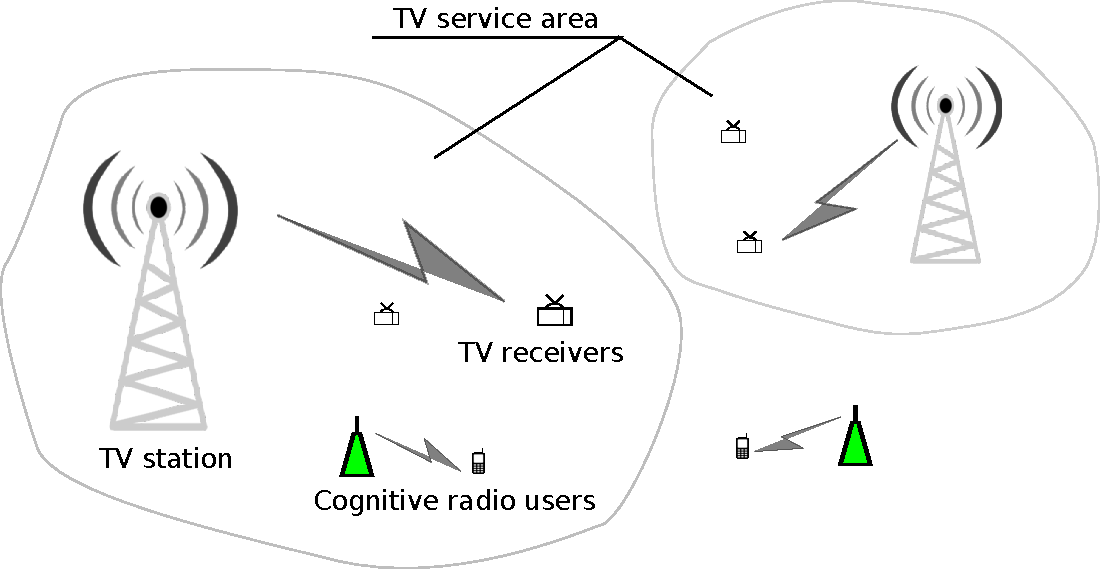
\includegraphics[width=0.75\linewidth]{underlay.pdf}
	  \caption{The concept of overlay spectrum usage in a TV service scenario. The hull shows the range of a TV service area, inside and out of which secondary users work on the licensed channels.}
	\label{underlay}
	\end{figure}


\item \label{overlay} Spectrum overlay:
The other approach is \textit{spectrum overlay}, where secondary transmitters are only allowed to transmit when the primary users are detected as being idle, and the spectrum should be vacated if a primary user is detected transmitting.
Working with this paradigm, secondary users should monitor the spectrum of interest pre-actively to detect primary users' appearance.
This kind of spectrum sharing strictly protects the primary users, but entails burden on secondary users especially on the aspect of spectrum sensing.
The detection metrics include received primary users' signal power, spectral correlation or beacons~\cite{crnsensing_09}.
Spectrum sensing requires sophisticated technologies when primary users' signal is weak, and can be improved by learning technologies or cooperation among multiple secondary users~\cite{coorperativeSensing_Akyildiz11}.
When spectrum sensing accuracy can be guaranteed above certain threshold, transmission power restrictions can be removed from  secondary users.


\end{itemize}



\subsubsection*{Spectrum sharing among the secondary users}
Among the secondary users, there is also competition on transmission power, spectrum bands or transmission time slots.
When we put the consideration on protection of primary users aside, spectrum sharing among the second users is similar with the counterpart problems in the conventional wireless networks, \ie ad hoc networks, cellular networks, etc..
In CRN, spectrum sharing among the secondary users can be conducted with either cooperative or non-cooperative manner.
As to cooperative spectrum sharing, secondary users take into consideration of the caused interference on other secondary users when deciding their spectrum usage.
This pattern usually requires cluster structure to facilitate the negotiation of users in a neighbourhood~\cite{Chen07}.
Whereas with non-cooperative spectrum sharing, secondary users only consider the performance of their own.



%Secondary users' operation is restricted on certain spectrum bands and transmit power should be below certain threshold according  to their locations, and spectrum sensing ability is also required.





\subsection{Operation Models of Spectrum Sharing in CRN}
From the perspective of network operation, spectrum sharing can be classified as centralized and distributed spectrum sharing.

%Centralized spectrum decision doesn't work well outside the TV channel scenario.

\subsubsection*{Centralized Scheme}
Centralized spectrum sharing is conducted on a centralized entity to decide the secondary users' strategies to operate in the CRN.
There is a considerable number of centralized approaches proposed for spectrum sharing in cognitive radio network, and the global optimality is reported as to different objectives in certain cases.
%
The centralized solution is usually realized by formulating the communication problems into optimization problems.
Let us take the resource allocation problem in CRN as example.
The resource refers transmission power, spectrum, transmission time, etc..
The objective can be the following, improving the overall SINR of secondary users, mitigation of co-channel interference caused secondary users, minimization of transmission power, etc,.
The constraints can be one or several of the following, the interference caused by secondary users on primary users is below a threshold, the transmission power is restricted by the maximum transmission power, or the number of spectrum bands allowed for secondary users to use.
There is a good number of research in this regard~\cite{resource_allocation_crn_Ahmad_2015}~\cite[Chapter~6]{Han:2008:RAW:1457343}.
%There has been a good number of works in this regards~\cite[Chapter~6]{Han:2008:RAW:1457343}.

When the formulated problems are linear programming, or convex programming problems, the optimal is easy to obtain.
When convexity doesn't held, there all some skills to convert the problem into convex ones, \eg a $\log$ change of variables turns an apparently non-convex problem into a convex one.
When integer variables are involved in the optimization, \eg in problem of channel assignment, or scheduling, the optimization problem is very difficult to solve.
In this occasion, swarm intelligence algorithms can be applied to obtain sub optimal result.
simulated annealing [xxx], generic algorithm [xxx] and ant algorithm etc.

Centralized scheme is suitable in certain scenarios, \eg when the primary users are TV stations and receivers which work on certain channels for hours of time, spectrum can be seen as constant. 
When the secondary users access the spectrum in underlay paradigm, they need to take care not to cause more interference than threshold on primary users.
In this case the channel usage, \ie working channel and transmission power, can be decided on the centralized controller.
%
Nevertheless, centralized solution is not suitable in many scenarios of CRN.
First, central authority or controller is not available in many CRNs, \eg CRAHN.
Second, when the centralized decision maker exists, centralized solution involves a large number of control messages during network operation.
The centralized entity needs to collect spectrum availability sensed on all the secondary users, then computes the spectrum usage strategy before finally distributing the result back to every secondary user.
When primary users intensely access the spectrum and result in frequent change of available spectrum, the control overhead becomes a burden for the CRN.
Third, Centralized solution need to react to the spectrum variance in the CRN, even when the spectrum changes only happens at a few secondary users.
This compiled agility worsens the overhead problem.
%, and it is different for the centralized entity to obtain a full and up to date picture of the spectrum availability in the whole network.



%In wireless networks, signalling is performed to conduct resource allocation in an optimal way, which causes considerable overhead in communication.


%As to cognitive radio network, implementation of centralized algorithm faces more challenges.
%The central controller needs to know the network connectivity which is decided by the availability of licensed spectrum, or even the information of the later.
%Either the controller enquiring each secondary user for spectrum availability information, or the secondary users pushing to the controller introduces huge amount of overheads, especially when the primary users change their operation state frequently
%When the licensed users change their operation state frequently, centralized decision maker obtaining the updated sensing results from CR users imposes a great burden on the network.
%In this case, it is also possible that the centralized controller is only responsible to regulating the maximal transmission power to protect the licensed users from interference, but doesn't control secondary users' transmission strategy as they may belong to different business groups.

%Without infrastructure support, it is hard for CR user to get complete and up to date picture of the spectrum availability in the whole network.
%Thus distributed solutions are preferred in such varying radio environment.
%Distributed decision of one CR user should be carefully decided as one CR's behaviour affects neighbouring CR users which go on to prompt all the CR users in the network to act accordingly.

\subsubsection*{Distributed Scheme}
It is the primary users which distinct CRN from other networks.
Primary users' usually unexpected operation pattern results in dynamic spectrum availability for secondary users.
As distributed schemes exploit mainly local observation, distributed schemes help the secondary users to adapt to the varying environment quickly~\cite{Selforganization_CRN_13}.

Distributed solutions generally don't involve large amount of control overhead.
When working with distributed spectrum sharing paradigm, secondary users in CRN decide on their spectrum usage strategies autonomously based on the local information, \ie either on themselves or from their neighbourhoods.
Consequently, distributed scheme usually requires secondary users to exchange information \ie user ID, channel availability, etc. only with their neighbours, as a result, the overhead involved in the network is reduced.
It is reported that control overhead takes account more than 50\% of messages in most networks~\cite{Han:2008:RAW:1457343}.
When the overhead is decreased, spectrum utilization and the number of served users and the network performance can be correspondingly improved.

%
In certain scenarios, distributed scheme may also make use of centralized entity when it is available and necessary, \ie secondary users can access the centralized database to retrieve the available channels in IEEE 802.22 cellular networks.

%Signalling overhead is even more considerable as the channel state varies due to primary user activity.
%Thus the distributed scheme is more suitable than cognitive radio networks than other wireless networks.
Although distributed scheme results in appealing lightweight computation and overhead, it is actually challenging to design in many scenarios.
When the distributed decision is not properly designed, it is possible to trigger endless ripple effect across the network, \ie one CR's decision on its strategy prompts neighbouring CR users to change strategies, and it changes its strategy again later due to neighbours' new strategies.
%
The distributed schemes designed for CRN can be roughly classified into the following categories.
\begin{itemize}
\item Distributed schemes which are derived from optimization formulation through decomposition.
This method secondary users use local information, but together achieve global optimal.
This method requires the optimization problem to be convex, thus it can only solve a small portion of spectrum sharing problems.
%\item Heuristic methods.
%Back in 
% local bargaining~\cite{localBargaining_05}
\item Online learning.

Online learning lies in the domain of artificial intelligence. 
The application of online learning in spectrum sharing in CRN includes Q-learning~\cite{reinforcement_learning_crn_wcnc_2013}, no-regret learning~\cite{hart00correlatedeq,qlearning_huang}, reinforcement learning~\cite{reinforcement_learning_crn_2011}.
Operating with this method, each secondary user seeks for suitable resources to maximize its utility function.
Secondary users' operation is in distributed and asynchronized manner, and the CRN ceases to update in a correlated equilibrium.
online learning has appealing property on distributed execution, but the convergence speed can not be guaranteed.
\item Game theory.

In comparison with optimization which seeks to improve the welfare of the complete network, game theory sheds light on the individual entities in a system.
A game can be seen as a collection of optimization problems, each of which maximizes/minimizes the utility/cost of one individual entity in the system.

Actually, a distributed scheme can be regarded as a non-cooperative game formulation. 
Under the game theoretic framework, we can analysis the interaction among the users operating according to the algorithm.
Then We can check whether the system reaches a desirable equilibrium, \ie the individuals also improve the global welfare of the complete system.
We can also inverse the procedure to help solve our problems in CRN.
Given a known game which holds preferred properties such like fast convergence to equilibrium, or the game only has a single equilibrium which is also the global optimal, we can formulate our problem into that kind of game, then modify the best response of the players as the distributed algorithm for the communication entities in our problem.

We will introduce the application of game theory in CRN in the following section.

\end{itemize}
%Game theory is a suitable tool for analyses secondary users in CRN, and from which derive algorithms. 


%because it is costly to retrieve necessary information from the network to the controller, which includes the spectrum information on each CR users and the network topology. Besides, when the solution is sent back to the CR users, the network state may have changed and be different from the time when the information is collected.

%This is due to the operation of primary users, which is usually not known by secondary users.
%The distinctive view on spectrum availability and varying radio environment make distributed solution a natural choice for CRN network.




%Aforementioned classifications correlate with each other in certain aspects.
%For instance, non-cooperative spectrum sharing is usually conducted in distributed manner, whereas cooperative spectrum sharing can be implemented in both distributed and centralized manner, and the later needs the assistance from the centralized entity.

%Spectrum sharing scheme need to be designed according to actual requirement and available facilities.


%The forthcoming vehicular to vehicular communication requires

%Based on the type of primary system which CRN underlays to co-exist, the availability of licensed spectrum exhibits variations on temporal and spatial aspects.



%However, the autonomous operation of secondary users always comes with a residual risk that primary systems are not detected despite their reappearance. Hence, other approaches to primary detection have been proposed relying on geolocation and database (DB), where secondary users are told by a centralized database about the spectrum availability with a time dimension. In this concept, the transmission power can also be controlled by the database. After obtaining the available spectrum to use, the secondary users need to decide which chunk of spectrum to use so as to satisfy the QoS requirements for the service it conveys. In order to achieve good performance, secondary users should be aware of the activity pattern of PUs, so that they can pro-actively plan the spectrum usage. Finally, SUs need to share the spectrum with other SUs, thus interference mitigation is an important issue to be considered.

%Whenever primary users are detected, the secondary users have to either jump to other spectrum, or turn down its transmission power to avoid interfering the primary users.





\section{Game Theory and CRN}
Game theory is a branch of applied mathematics, and it is a powerful mathematical tool for studying, modelling and analysing the interactions among individuals.
As to one same problem, the approaches derived from game is complementary to the optimization method.


A game consists of three tuples: a set of players, a selfish utility for each player, and a set of feasible strategy space for each player.
In a game, the players are rational and intelligent decision makers, which are related with explicit formalized incentive expressions (the utility), and usually they have potential conflicting objectives with each other.
We say the players are rational as they make decisions in compliance with the subjective which is either to maximize the expected utility, or to minimize the expected cost.
Player are intelligent as they understand the other players are also rational.
%
Game theory provides standard procedures to study its equilibriums~\cite{game_for_communication_01}.
The most frequently used concept of equilibrium in game theory is Nash equilibrium (\gls{NE}).
NE defines a stable state of the system, where with the given policies, no player may gain by unilaterally deviating its current strategy.



When the network entities are seen to be self-interested rational, suitable game theoretic models can guide the behaviours of them, so as to achieve desirable collective behaviours and performance with respect to the system level objective.
A NE in CRN means the CR user has no incentive to change its operating parameters \eg transmission power, spectrum band, time slot, modulation, etc.. 


In the past few years, game theory has been extensively applied to problems in communication and networking~\cite{Neel06analysisand, Wang_gtc_crn_survey_2010}.
Game theoretic models are used to understand many challenging problems in communication systems, such as resource allocation, topology control, routing, security and so on. 

%In recent years, game theory attracts people attention into apply it in communication systems.
We list the reasons to apply game theory in communication systems.
\begin{itemize}
\item \textbf{Communication equipments are rational.}
Although current communication equipments involve only a little artificial intelligence, they are supposed to be manufactured and operate based on standards to fulfil certain functions, but selfish behaviour may appear on certain individual equipments to achieve advantages over their peers~\cite{game_for_communication_01}.

In communication system, a device is programmed to maximize the expected utility, which is perfectly rational.
For instance, Wi-Fi equipments are manufactured complying the IEEE 802.11 standards.
But it is possible that certain manufacturers or the personal who uses the Wi-Fi system (we use station in the following) manipulate certain parameters to obtain performance advantage over other stations in the network.
When all the stations in one network are supposed to run distributed coordination function (\gls{DCF}), \ie the station must wait a random period of time, which is called contention window (\gls{CW}), before accessing the media when it senses the media to be busy, a certain selfish station may not choose to wait and is keen on sensing media.
The selfish behaviour causes more collisions for other stations, and possibly results in poor performance in the network.
%In this case, the access point finds more packets coming from that selfish user, but is unaware of its selfishness and has no means to adjust or punish this selfish user.
In this case, game theory facilitates the network operator to issue rules to make the selfish behaviour unprofitable, or it helps to analyse how much the impact can be caused by the selfish stations.
% can tell the access point or network operator the impact caused by the selfish systems, and possibly 

\item \textbf{Game theory is effective to solve networking problems.}
Algorithms can be retrieved from the analysis of a problem under the game theoretical framework.
In the same example of media access in IEEE 802.11 DCF mentioned in the previous item, if stations are allowed to modify the length of contention window, each station will adjust its contention window to obtain the best performance.
\cite{contentiongame_07} shows as long as each station greedily updates its CW to maximize certain utility, after certain time the system will stabilize in NE. 
In the case, the best response process naturally defines an algorithm for Wi-Fi systems.
%
Besides, outcome from game theory is robust~\cite{Han:2008:RAW:1457343}.


\item \textbf{Game theory is suitable to apply in cognitive radio network because of the properties of CRN.}
Firstly, as only local information is needed to feed each user, game theory is naturally suitable for designing distributed solutions for cognitive radio networks.
Distributed solutions doesn't rely on centralized controller, and each user in the network adopts certain action as response to the other users or environment, this falls in the scope of game theory.
Distributed schemes usually lead to Nash equilibrium, which is usually sub optimal.
As comparison, although optimization is the common tool to pursue global optimality, when the information is not accurate or adequate enough, or the optimization itself is difficult to solve, the optimized results can be far from optimal.

%
Secondly, combinatorial nature of communication problems makes game theory as one of a few choices~\cite{Han:2008:RAW:1457343}.
Many problems in wireless communication involve integer variables, \ie channel availability, channel assignment, selection of modulation levels or channel coding.
It is always challenging to solve combinatorial optimization problems, whereas game theory is natural to describe it in a discrete form.

\end{itemize}

In this dissertation, we look into congestion game and its application in CRN.


\subsection{Game and Congestion Game}
The most frequently used concept of equilibrium in game theory is Nash equilibrium.




\subsubsection*{Congestion Game}
In accordance with~\cite{Voecking06congestiongames}, congestion game is a game where players simultaneously allocate sets of resources to minimize their costs, and the cost of a resource is a function of congestion, which is the number of players choosing the resource.
Congestion games can be formulated from many problems in realistic world, \eg minimisation of commuting time on the road for commuters, minimization of energy consumption in mobile cloud computing system~\cite{game_cloudcomputing_energy12}.



\section{Representative Cognitive Radio Networks}
In this section, we introduce two types of cognitive radio networks, and the problems we tackle in this thesis reside in these networks.

\subsection{Cognitive Radio Ad Hoc Network}
%An ad hoc network is a decentralized paradigm of wireless network, which consists of a collection of autonomous mobile users which communicate over wireless links.

%Efficient distributed algorithms are needed to determine network organization, link scheduling, and routing.

Cognitive radio ad hoc network (\gls{CRAHN}) is composed with autonomous mobile cognitive radio users which work with overlay spectrum sharing paradigm.
CRAHN is one mobile ad hoc network, whereas each mobile user has cognitive ability for spectrum access.
Mobile users in CRAHN need to determine which channels are available to use with spectrum sensing, either cooperatively with neighbour users or individually.
Mobile users have different knowledge of spectrum availability, which poses new challenges in addition to the ones for the management of mobile ad hoc network.
CRAHN can be usually represented by an undirected graph $G$.
Cognitive radio users constitute the vertices, the edge between two vertices is decided not only by the distance, propagation and attenuation properties between the two vertices, but also the spectrum availability on both vertices, \ie when they can decode the received signal from each other correctly, and there is common channel available between them on which communication is conducted, then an bidirectional edge is available on graph $G$.
As to ad hoc network, the graph is constant when users are static.
As to cognitive radio ad hoc network, due to primary users' activity, an edge between two vertices is decided by the fact that whether the two vertices can simultaneously access the same licensed channel.
Hence, the corresponding graph is dynamic under primary users' operation, which imposes extra difficulties on network organization, routing and many other network functionalities.

%\subsection{IEEE 802.22 Standards}
%\label{ieee80222}%XXXXXXXXXXXXXX clearly statement, regulations of FCC, ECC, 802.22 XXXXXXXXXXXXXXXXXXXX
%%%XXXXXXXXXXXXXXXXXXXXXXXXXXXX   paper: IEEE 802.22: The First Cognitive Radio Wireless Regional Area Networks (WRANs) Standard
%IEEE 802.22~\cite{802.22} is the standard for Wireless Regional Area Networks (\glspl{WRAN}), which defines a cellular network paradigm for secondary equipments working on unused TV channels in overlay manner.
%Unused TV spectrum is termed as TV White space by the Federal Communications Commission (FCC)~\cite{FCC_2010_sedond_memorandumm}, which is licensed to incumbent users such like digital TV, analog TV, and wireless microphone.
%As the TV service is transferred from traditional analog to digital, the
%The TV channels to be used are of UHF/VHF TV bands and are between 54 and 862 MHz.
%The bandwidth of one TV channel is 6 MHz.%XXXXXXXXXXXXX add some description in details XXXXXXXXXXXXXXXXXXXXXX
%
%
%Unlicensed users consists of White Base Stations (\glspl{WBS}) and customer premises equipments (or terminals for short), where each terminal is served by one base station. 
%As to unlicensed users, detecting incumbent users is challenging because the FCC requires the unlicensed users should be able to detect the presence of signals from TV stations or wireless microphone at a received power level of -114 dBm~\cite{Technical_Challenges_TVwhit}. 
%Thus FCC doesn't require the sensing ability on unlicensed users, but regulates the secondary usage of TV white space in a prudent manner, including the spectrum bands permitted to use based on their location, the transmission power, the distance away from TV service area and so on.
%IEEE 802.22 largely complies FCC regulations on the utilization of TVWS.
%
%There exists a centralized database, and every unlicensed user should register its type and geographic location to one TV database.
%The centralized database notifies the secondary users the available spectrum at their places, and is possible to decide transmission parameters for them, \ie spectrum to be used, or transmission power.
%Note this database takes the functionality of spectrum sensing in addition to spectrum decision and sharing, thus IEEE 802.22 adopts centralized spectrum decision for unlicensed users.
%The feasibility of this centralised paradigm is largely due to the characteristics of TV channel, as TV channel usage follows a slow and scheduled pattern. 
%When two or more base stations operate on the same channel, TDMA like mechanism for WBSes is adopted.
%%Centralized spectrum decision is adopted in IEEE 802.22.
%
%
%Recent standard published in Nov. 2010 suggests both sensing ability as well as database look-up to avoid affecting primary systems.

\subsection{Cognitive Radio Cellular Network}


\subsection{CRN Working with TV White Space}
\label{TVWS}
%Opportunistic utilization for unlicensed secondary users (also named as white space devices, abbreviated as WSD) working with TV broadcast spectrum (TV white space) is promising to cope with the scarcity of spectrum resources\cite{fcc}. 
%UHF TV spectrum (TV white space, TVWS) has low utilization in both spatial and temporal dimensions. \fmjg{xxx relevant data and citation needed here XX also mention where this is the case, i.e. US ? XXX}


TV white space (\gls{TVWS}) refers to the unused broadcast television spectrum.
One part of the unused TV spectrum is resulted from the switchover of analog television to digital television, which frees up a large range of TV spectrum.
The other parts are unassigned spectrum and the spectrum which is not being used at a given time in a given geographical area.
TV white space is located in the VHF (54-216 MHz) and UHF (470-698 MHz) bands, thus the frequency bands within this spectrum are highly desirable for wireless communications, because they have good properties on propagation, \ie they have broadband payload capacity, and are able to penetrate obstacles such as trees, buildings, and rugged terrain in non-line-of-sight scenarios.
As comparison, a Wi-Fi router's transmission range, which uses 2.4 GHz radio frequency and complies with IEEE 802.11, is around 100 meters under perfect conditions, and the signals can be blocked by barriers, whereas, TVWS band can cover an area of about 10 kilometres in diameter.
In 2010, FCC allowed~\cite{FCC_2010_sedond_memorandumm} unlicensed devices to operate in the TV white space to provide broadband communication for consumers and business.
%On November 4, 2008, FCC made far reaching changes on spectrum usage by opening the unused portion of the UHF TV space to unlicensed secondary users. 
%\textit{Unused portion} here denotes the TV spectrum which is not currently being used by TV stations, or that secondary users can use while the ongoing TV broadcasting on the same spectrum is not interfered.
%These unused portion of TV spectrum is called TV White Space (\gls{TVWS}).

Autonomous spectrum sensing is one approach for secondary users to decide the available TV spectrum. 
Secondary user scans certain parts of the TV spectrum band to detect the presence of existing TV equipments with advanced spectrum sensing techniques and algorithms.
This scheme involves complex sensing techniques, and it doesn't work well in worst case sensing scenario, \ie the TV receivers are hidden nodes~\cite{maximum_power_TVWS_dyspan_2011}.
%However, to prevent any interference with ongoing TV broadcasts, the sensing algorithm becomes quite complex. 
Moreover, it is required to be conservative when deciding the available TV channels leading to an underestimation of available TV channels and causing inefficiencies~\cite{geoTVprotection08dyspan}.
Considering the slow change of TV spectrum usage, along with the fact that the spectrum usage by TV stations is scheduled, the geolocation approach together with central database becomes more appealing in TVWS utilization scenario.
FCC adopts this solution as the main way, and regulates the secondary usage of TV white space in a prudent manner, including the spectrum bands permitted to use based on their location, the transmission power, the distance away from TV service area and so on.


FCC regulates portable secondary users to operate from channel 21 (512 MHz) to 51 (698 MHz), with the exception of channel 37.
As to the fixed secondary users, the allowed spectrum band is from TV channel 2 (54 MHz) to TV channel 51, with TV channels 3, 4 and 37 being prohibited.
Thus, the available TV spectrum is about 600 MHz wide. 
Compared to conventional unlicensed ISM bands in the 2.4 GHz and 5 GHz band, all together TVWS has more to offer.
%xxx While the TV spectrum is free to use under the above mentioned conditions, it might also be 'polluted' by primary TV stations due to the coexistence with them. xxx
\cite{DySpAN10MeasuringWhitespaceCapacity} analyses the capacity possibly provided by exploiting free TV channels. 
Complying with the rigid regulation of FCC, TV white space brings hundreds of kilobits/sec per square kilometre for secondary users when the communicating secondary pair is about 1 km apart.
The research shows that interference from TV stations and other co-channel secondary users heavily restricts the capacity.
\cite{tvgreyspace12} further investigates the possible TVWS usage \textit{within} TV service area (referred to as \textit{gray space}), where the secondary usage does not violate TV receivers.
The authors propose another significant amount of TV spectrum, but the interference from TV broadcasters is stronger due to the secondary receivers being closer to TV broadcasters. 

The potential applications supported by TVWS are the major driving force for TVWS communications technology.
It is envisioned that TVWS can support high-data-rate backbone for fixed stations in large area connectivity, short-range indoor connectivity, seamless connectivity for mobile stations and emergency related equipment. 
In the following, we give a brief introduction to the governing regulations and industrial standards issued for TVWS usage.




%Firstly, more unused TV white frequencies become vacant than ever with the ongoing transition from analog to digital broadcasts. Secondly, the lower frequencies of TV band enable broadband access over much longer ranges compared to other bands with higher center frequencies. TV white space contributes an alternative to industrial, scientific, and medical (ISM) band which is already heavily congested. Besides, TV white space provides abundant spectrum resources for cellular network, so that the frequency reuse factor is decreased and sophisticated interference mitigation mechanisms can be alleviated. TVWS is free but with restrictions, TV receivers should be protected from the harmful interferences form WBDs, in other word, the aggregated interferences caused by all working WSDs should not exceed a threshold on TV receivers.



\subsubsection*{Co-Existence in TV White Space}
%In compliance with the methodology of cognitive radio, 

%this is a intro to a general cr work.
%Temperature regulation~\cite{Temperature_regulation03} opens another way to utilize TVWS. \cite{wuinfocom09} deals with the joint channel-power selection for multiple transmission links (pairs) in a general cognitive radio scenario. The distributed scheme is derived from decomposition of Lagrangian dual, which converges pure Nash equilibrium. To facilitate this scheme, monitors from TV stations are required to watch interference from WSDs, furthermore, monitors have to be equipped with computational ability and interact with secondary users in the whole process of convergence. This methodology works in try-error-try mode, which asks for modification on the current operation of TV services.
Regulatory bodies in different countries have issued requirements on the occupancy of TVWS bands by secondary users respectively. 
The permitted channels regulated by FCC have been briefly introduced above.
Besides, FCC divides the devices operating in the TVWS (TV band devices, or \glspl{TVBD}) into three categories: Fixed device, Mode I personal/portable device, and Mode II personal/portable device. Every category obeys distinct rules on transmission power, mandatory database access and so on.
Fixed and Mode II devices are connected to the database directly (or indirectly by another fixed or Mode II TVBD), Fixed device accesses DB at least once per day, Mode II device has to access DB every 60 seconds, or when it changes location by more than 100 meters.
The transmission power for Fixed TVBD is 4 W, and 100 mW for Mode II TVBD. 
Mode I TVBD operates only under the control of a fixed or Mode II TVBD, and accesses them for available channels every 60 seconds.
There is also regulations on the antenna heights and other aspects.
OFCOM (being the regulatory authority in UK) opens less TVWS for TVBD and categorizes White Space Devices (WSDs) into Master WSD and Slave WSD which are roughly equivalent to fixed/Mode II TVBD and Mode I TVBD, respectively.
ECC (being the regulatory authority in Europe) also adopts Master and Slave structure while utilizing the geolocation and database solution to assign channels and corresponding operating parameters to TVBD.
In both FCC and ECC regulations, the available channels are calculated based on the distance between primary and secondary systems together with some propagation model.
Hence, the principle behind the notion of channel availability is the presumed received signal strength at potential TV receivers, which should be obviously below a certain level.
FCC adopts a fixed transmit power level for secondary systems and assumes that the distance used (resulting from the propagation model) is sufficient to protect the TV receivers.
ECC's restriction is more flexible on the transmission power which can be adjusted based on the distance between the secondary user and the TV receivers. 
For both regulations, TV receivers may become vulnerable when there are multiple secondary equipments transmitting simultaneously.
\cite{Jaentti11} shows that even the regulations integrate an interference margin for multiple secondary users' transmitting, the TV receivers are still vulnerable.

%
%Some regulations, as that from FCC and ECC, are sufficient guidance for actual implementation, while some other rules are providing test for interference assessment. 
%
Standardization on secondary usage of TVWS is very active. IEEE 802.19 is a family of IEEE 802 standards in Wireless Coexistence Working Group, among which, IEEE 802.19.1 is for wireless coexistence in TVWS. IEEE 802.11af is standards for WLAN operation in TVWS, IEEE 802.15.4m is for low rate (LR) WPAN operating in TVWS. IEEE 802.22 is for Wireless Regional Area Network (WRAN) using TVWS. As TV band is only 6 or 7 MHz while WLAN channel bandwidth is 40 MHz for state-of-the-art IEEE 802.11n amendment, IEEE 802.11af proposes channel aggregation mechanism for WLAN working with TVWS. Maximum transmit power and spectrum mask of Mode I should be approved by Mode II devices beforehand.  


%Geolocation is extensively used in cognitive radio network. \cite{nashbargaining_2012jsac} proposes a centralized light weighted scheme to solve channel and power allocation among secondary users with TDMA manner, where geolocation of primary users are used by secondary users to calculate the caused interferences by them on the primary users. Considering the slow change of TV spectrum usage, along with the fact that the TV spectrum usage is scheduled, geolocation approach becomes more appealing in TVWS utilization scenario. Assume there is a database which is connected with all WSDs, and it is aware of the location of TV receivers (optionally with terrain information) and WSDs and proper propagation model in between, the database calculates the RSSI (Received Signal Strength indication) on each WSDs in the whole network. The database decides the channel availability based on whether the RSSI exceeds a threshold value or not, then notices WSDs their available channels in either proactive or reactive manner. This geolocation approach is used for building a Wi-Fi like network working with TVWS ~\cite{SenseLess} which demonstrates the feasibility of predicting the available TV spectrum accurately using suitable propagation models (Longley-Rice and terrain wherein). This approach is also integrated into regulation from Federal Communications Commission (FCC) of U.S. FCC regulates every WSD should access the database to retrieve the available TV channels on its location, and fixes the transmission power for fixed WSD as 4 W which is a conservative value. Aforementioned is calculation RSSI of PU on the location of WSDs to see whether the PUs \textit{appears}, there is another way to work with geolocation. Instead of deciding the available TV channels for WSDs, database calculates the interferences from WSBs on TV receivers, then directly assigns channel and power levels to each WSD and in the same time preventing the TV receivers from harmful interferences (the interferences under a certain threshold). Electronic Communications Committee (ECC) in Europe adopts this approach so that the transmission power for WSD is more flexible depending on WSD's location.


IEEE 802.22 has been the first IEEE standard for wireless regional area network (WRAN) working on TV white space. According to this standard, the system consists of a base station and customer premises equipment (or terminals for short), where terminals are associated with base stations, and are served by them. Recent standard published in Nov. 2010 mentions both, i.e. sensing ability as well as TVWS geolocation and database look-up as schemes for detecting primary systems. Self-coexistence mechanism is also proposed, which provides a TDMA like mechanism for WBSes to share TVWS. \cite{HoangPowerChannel2010} proposes a distributed solution for power control and channel assignment in both down-link and up-link communication in a WRAN, but the investigated secondary network is composed with only one base station and multiple terminals. % Although the transmission power is decided in a distributed manner, primary transmitters are required to adjust their transmission power in order to guarantee the SINR on primary receivers in a learning process, while, the operation of WSDs working on TVWS should be transparent as to TV services.\fmjg{This summary of the 2010 paper does not make sense to me - why are you talking of primary systems here ??} 




\section{Problem Statement}
The xxx

Adopting centralized or decentralized solutions is largely dependant on the network types and desired services to convey.
%Working with the TV white space is regarded as one application of cognitive radio network, which is most likely to succeed in near future.
As to secondary users working with TV white space, regulations and standards desire one centralized database, which can be used to conduct certain centralized solution to assign the resources.
As to CRAHNs which consist of mobile autonomous secondary users and without any infrastructure, distributed scheme practically becomes the sole choice.
Actually, the majority of the research in cognitive radio domain is carried out with distributed manner.
%In CRAHNs, there are no centralized utility, and the spectrum sensing is necessary for every secondary user.

We proposes distributed solutions for a series of problems in cognitive radio networks.
We investigate the differences between decentralized and centralized schemes in terms of several criterion, \ie Performance, overhead and needed time.



In this thesis, the fundamental technical challenges to be addressed in this thesis are shown in Figure~\ref{problemLocation}, which reside from physical layer to network work layer~\cite{osi} are addressed. 


\begin{figure}[h!]
  \centering
  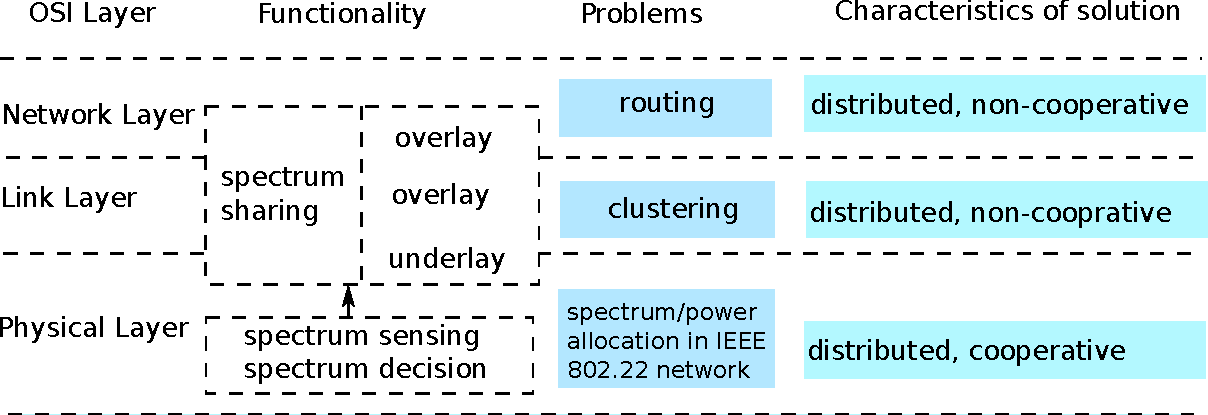
\includegraphics[width=\linewidth]{problemLocation.pdf}
  \caption{Spectrum management and the problems addressed in this thesis}
\label{problemLocation}
\end{figure}

%We focus on the distributed solutions for several correlated fundamental problems in CRN.
The interaction among autonomous secondary users is a common scene in CRN as there usually lacks central controller.
The secondary users endeavour to maximize their performance by choosing the channel and power, and meanwhile the accumulative interference caused on primary users should be below a threshold.
How to refrain the accumulative interference to exceed the threshold is a critical question, and whether the distributed decision made by each secondary user on channel and transmission power improves performance is worth considering.
After building the connected network with the chosen channel and transmission power, forming clusters with neighbours is a natural method to gain benefits, \ie more accurate spectrum sensing, from local cooperation.
How to form such clusters which can survive in front of the unpredictable activity of primary users is challenging.
Having had solid CRN infrastructure, it is time to deliver services via routing.
A light weight routing tailored for CRN is needed.
In the following, we give full problem statements for the mentioned challenges.



\subsection{Channel and Power Allocation in IEEE 802.22 Network}
%\subsubsection*{Utilize TV White Space}

 %Considering that secondary base stations are likely to be from different administrative domains, a distributed solution would be required. And that makes us turn to game theory and the separation of the problem into two different ones. 


%As introduced in Section~\ref{ieee80222}, the TV white spectrum has appealing characteristics for secondary users, for instance, the TV spectrum spans wide frequency range, it is not used by TV services frequently and the spectrum availability lasts relatively longer.
There are several problems with the current regulations and standards proposing on the utilization of TVWS.
Firstly, most of these proposals rely on the centralized database to manage the spectrum usage in a centralized manner.
This paradigm is not suitable when the TVBD belong to different business bodies, \ie operators.
Thus, a centralized resource allocation is infeasible.
Secondly, the current usage of TVWS is prudent, \ie on working channel and transmission power as introduced in Section~\ref{TVWS}.
These conservative measures on the transmission power restrict the full utilization of TV spectrum.
Thirdly, as the transmission power of TVBD is restricted, the interference between TVBDs is not given consideration.
In fact, as the interference caused between co-channel transmitters may not be symmetric, the solutions proposed for the channel assignment problems in conventional networks, \eg ad hoc networks, or mesh networks can not be applied any more.
%As to the former problem, based on the information of geographic locations and attenuation parameters, the upper bound of transmission could be relaxed, and the centralised database is a suitable place to conduct this work.
%The later problem, at the first glance, has many similarities with the channel assignment problem which has been discussed extensively in the past decades, but the problem is unique as the transmission power on each user is different.
Up to our knowledge, there is no work coping with co-existence between secondary base station with both primary TV broadcasters and other base stations.

%Each base station working with TVWS needs a certain transmission power and a certain spectrum.
%The decision should maximize performance of terminals in this cell under interferences from TV broadcasters and other secondary base stations, meanwhile, the TV receivers should be protected.


In this thesis, we propose a solution for the joint power and channel allocation problem for the base stations in a WRAN network.


%This is very applicable as TV spectrum usage changes slowly, and the spectrum usage by TV stations is scheduled.
%the geographic location approach together with central database becomes more appealing in TW White Space (TVWS) utilization scenario. 
% FCC regulates portable secondary users to operate from channel 21 (512 MHz) to 51 (698 MHz), with the exception of channel 37. As to fixed secondary usage, the allowed spectrum band is from TV channel 2 (54 MHz) to TV channel 51, with TV channels 3, 4 and 37 being prohibited. Thus, the available TV spectrum is about 600 MHz wide. Compared to conventional unlicensed ISM bands in the 2.4 GHz and 5 GHz band, all together TVWS has more to offer.


\subsection{Robust Clustering in Ad Hoc Cognitive Radio Network}
Clustering is an important paving stone for the practical utilization of the unused portions of the licensed spectrum.
Clustering secondary users based on geographical proximity and other relevant properties together produces following benefits.
Firstly, it is more efficient to solve common control channel (\gls{CCC}) problem with cluster structure.
Dedicated CCC which is allocated to all nodes for the purpose of control information exchange is regarded to be under utilization.
Whereas, cluster based approaches group CR nodes into clusters based on their similarity of available unlicensed channels, so that the common channels within each cluster are used to carry the control messages~\cite{Lazos09}.
%whereas communication rendezvous, \ie the process to establish control channel between two CR users before they can communicate is proposed to be a economic solution.
%Within one cluster which is composed with CR nodes with similar available unlicensed channels, communication rendezvous can be accomplished within in shorter time~\cite{CommunicationRendezvous_ToN13}.
Secondly, cluster structure facilitates cooperative sensing and increases the sensing reliability~\cite{Sun07_clustering_spectrum_secsing}.
Thirdly, cluster structure supports coordinated channel switching and simplifies routing in ad-hoc cognitive radio networks~\cite{cluster_routing_2013ICC}.

The problem is defined by the following two metrics.
\begin{enumerate}
\item Abundance of control channels within cluster should be achieved.
A large number of control channels within cluster means high robustness.
When the current control channel gets occupied by primary user, cluster members can migrate to a new one and the cluster is maintained.
Besides, more control channels makes multiple concurrent transmission within cluster possible.
In this thesis, a distributed clustering algorithm which is especially designed to support robustness under active primary users is proposed.
Related works~\cite{Zhao07,Affinity_clustering_09icccn,Consensus_based_clustering12,clustering_globecom11} fail to pay attention to this aspect.

\item New scheme should be light weighted so that re-clustering can be quickly conducted when previous cluster is destroyed by primary user's activity.
When all the common channels are occupied by primary users, cluster head selection and following procedure is conducted by the cluster members autonomously.
\cite{LIU_TMC11_2} targets large number of control channels within cluster, but it intriguers high complexity.


%\item Efficient channel allocation scheme within and among clusters is needed, so that communication rendezvous between two clusters is quick. 
%Communication rendezvous means the process to establish control channel between two clusters before they can communicate .
%\cite{LIU_TMC11_2} proposes channel allocation in round robin manner, but it causes long time on communication rendezvous.
%\end{itemize}
%
%These requirements will be fulfilled by the scheme proposed in this thesis.
\end{enumerate}

\subsection{Geographic Routing in CRN with Spectrum Aware Virtual Coordinate}

Recent measurement in~\cite{measurement_Palaios14} shows the spectrum occupancy doesn't have significant spatial correlations between different locations.
It follows that licensed spectrum is used by primary users heavily in some areas, whereas in the other areas licensed spectrum is available over longer timespan for secondary users to use.
It is obvious to see that a routing path is better to go through the areas where primary users occupation is lower, as this alleviates or avoids the burden to cope with the changing or totally occupied spectrum when forwarding packets potentially with latency requirements.
Geographic routing is a natural choice to realize this geography sensitive routing path.
Geographic routing is light weight regarding the determination of next hop, and achieves high scalability in various wireless networks~\cite{geoRouing-qos-2009}. %
Merely knowing the geographic locations of its neighbours and the destination, a node is able to locally choose the next hop which has the smallest distance to the destination.
%As a result, control messages for route discovery are not necessary, and since the routing state maintained per node is independent on the network size, geographic routing scales perfectly.
However, in CRN dynamic link state renders geographic routing unsuccessful since packets are forwarded to the destination along the shortest path rather than avoiding areas heavily influenced by primary users.
%Coordinates indicate not only the physical distance among SUs, but also the transmission opportunities in between could leverage the strengths of geographic routing even in CRNs.
considering the available spectrum is geographically heterogeneous, applying geographic routing alike routing schemes in CRAHN is appealing, but the supporting coordinate system is missing.





\subsection{Research Questions}
Based on he previous analysis on the current secondary spectrum exploit, we conclude the problems into three distinct research questions.
In the remainder of this thesis, we will provide answers to these questions.

\textbf{Question Q1 - How to make full use of the TV spectrum, using the widely adopted network structure, preventing interference above threshold on primary TV receivers, and improve the performance of the secondary users.}

\textbf{Question Q2 - How to make the secondary users to form robust clusters against primary users' unpredictable activity?}

\textbf{Question Q3 - How to make use of the statistic information of the spectrum availability, so as to realize light weight geographic routing in CRN.}




\section{Contributions}
Because of the characteristics of the problems, distributed schemes are adopted, and in order to coordinate the interaction between secondary users, game theory is used to formulate the problem and derive algorithms.
We illustrate the contribution of this thesis by addressing the aforementioned questions.


\subsection*{Contribution 1: Distributed Channel and Power Allocation in IEEE 802.22 Network}



In this thesis we cope with a special channel allocation problem where symmetric interaction doesn't exist, \ie transmission power is identical among CR users, or the propagation path loss is not symmetric. 
The asymmetry disables the heuristic distributed schemes provided in~\cite{Ko_DistributedCA}, and makes channel allocation problem not to fit into the congestion game model proposed in~\cite{allerton08_liu} which is the first paper to discuss channel allocation from the respective of game theory.
We innovatively formulate this problem in to a canonical congestion game by utilizing the centralized database in TV white space scenario, and derive efficient distributed channel selection strategy.
%and apply it on different cognitive radio networks.
%rethink channel allocation problem from the perspective of game theory, particularly,


This thesis addresses following two problems,
\begin{itemize}
\item Decide the maximal downlink transmission power.
Both FCC regulation and 802.22 standard try to make TVBD transparent to incumbent users, but as long as TV system is not affected, i.e. certain quality of service is fulfilled, the strict restriction on unlicensed users can be relaxed so that more TVWS can be provided~\cite{multipleIntf_pimrc11}. 
Abiding by the operation paradigm using data base, we investigate the maximal downlink transmission power for TVBDs by solving optimization problem where the cumulative interference on TV receivers is under a threshold.

\item Distributed spectrum allocation scheme for TVBDs.
According to 802.22 regulation, spectrum allocation is done centrally in TV database, this is not realistic when TVBDs belong to different economic interest groups, thus a distributed solution is needed.
We propose efficient distributed scheme to allocate the TV channels in order to improve the quality of service of TVBDs.
The major difference between our scheme and other spectrum allocation lies in that the downlink transmission power on different channel is different.
We formulate this problem into a canonical congestion game, and derive the distributed algorithm from the best response behaviour of the player in the game. 
\end{itemize}





\subsection*{Contribution 2: Light Weight Robust Clustering in CRAHN}
We propose a decentralized clustering approach, which is able to form clusters whose sizes are not far away from the desired size, and the generated clusters are more robust than other robust clustering scheme, \ie more secondary users residing in clusters against increasing affection from primary users.
Compared to previous work, our proposed scheme involves much less control messages, and the generated clusters are significantly more robust.
We formulate one procedure of the scheme into a singleton congestion game, which permits Nash equilibrium when CR users adopt  best response strategy. 
%building more homogeneous clusters with respect to their size and forcing nodes with a high connectivity degree to the border of a cluster (making the cluster therefore more robust regarding connectivity loss to its neighbor).
%For our scheme we can prove convergence in cluster formation phase and resolve ambiguities with respect to cluster membership in a game-theoretic setting. 
On the basis of proposed scheme, we propose a light weighted version of ROSS, which requires exchanging less overheads.
%We leave the channel selection undiscussed.







\subsection*{Contribution 3: Spectrum Aware Virtual Coordinates in CRN}


In this paper we propose SAViC, spectrum aware virtual coordinates for secondary users in multi-channel multi-hop CRN where secondary users are source limited.
Virtual coordinate is independent of real geographic position, but decided by certain properties of the media among nodes, for instance, link quality or hop numbers~\cite{gpsfree05infocom}.
The proposed virtual coordinate depicts the availability of licensed spectrum influenced by primary users, on top of which geographic routing decides the next hop with Euclidean distance metric, and unconsciously detours the primary affecting area, or cuts through the area with better access opportunity.
This routing paradigm imposes little computation and communication cost on secondary users after assigning virtual coordinate, besides, it doesn't need real geographic location which is employed in ~\cite{search_geo_routing_chowdhury, routing-crn-jsac12}.

This scheme is composed with two steps,
\begin{itemize}
\item Design virtual coordinates so that virtual coordinates of any two secondary users reflect both geographic distance and opportunistic spectrum availability between them.
We design them based on statistics of primary user’s ON/OFF states which are obtained from local spectrum sensing.

\item After deciding on the next hop, we adopt a lightweight heuristic method to decide which channel to transmit packet when multiple licensed channels exist in the network.


\end{itemize}

To summarize, as the Euclidean distance between two secondary users based on spectrum aware virtual coordinate reflects the availability of unlicensed channel in between from the angel of historical statistics, virtual coordinate contributes a large part to deciding on the on the next hop. 



\section{Outline}
The structure of this thesis is as follows.
In chapter 2, we introduce the tools used in solving the problems, \ie game theory and optimization. 
Chapter 3 introduces the work on utilization of TV white space.
The robust clustering problem is addressed in Chapter 4.
In Chapter 5, virtual coordinate based on geographic routing is designed and geographic routing runs on the top of it.
Finally, Chapter 7 concludes the thesis by summarizing our contributions and discussing the future work.





\chapter{BACKGROUND}
\label{background}
%Some mathematical techniques which are used to solve the problems in thesis are introduced in this chapter.
%Neel06analysisand

In contrary to game theory where players agree on an equilibrium via autonomous behaviours, optimization problem, which attempts to optimize the welfare of either one equipment or whole network, is usually conducted on a single decision maker.
In the following, we introduce some basics of game theory and optimization.





 

%\todo[inline]{expand: Introduction of game theory...}
\section{Introduction of Game}
%Game theory is established by Nash in xxxx, and is applied in network communication since xxx
In this section, we give a brief introduction of game theory and congestion game which is applied to solve problems in the dissertation.
The notations used in this thesis comply with~\cite{agt_book}.


%\subsubsection*{Strategic Game}

A game of normal form can be represented as a tuple $\Gamma = (\mathcal{N}, (\Sigma_i)_{i \in \mathcal{N}}, (u_i)_{i\in \mathcal{N}})$, where 
\begin{itemize}
\item $\mathcal{N}$ is a finite set of players.
\item $\Sigma_i$ is player $i$' set of strategies.
Player $i$ selects one strategy $\sigma_i\in \Sigma_i$ at one time to play the game.
\item $\Sigma = \Sigma_1\times\cdots\times \Sigma_n$ is the set of states, which denotes all the possible ways that players may pick strategies.

\item $\sigma=(\sigma_i,\cdots,\sigma_n)$ is one strategy, which represents an instance of all players' strategy choices.
$\sigma$ is also called one strategy profile, and there is $\sigma\in \Sigma$.

\item One vector of strategies of player $i$' opponents is expressed as $\sigma_{-i}$, and the corresponding strategy profile is denoted as $\sigma=\{\sigma_i, \sigma_{-i}\}$.
$u_i(\sigma) = u_i(\sigma_i, \sigma_{-i})$ is the player $i$' outcome in strategy profile $\sigma$.

\item $u_i: \Sigma\rightarrow \mathbb{R} $ is the utility function of player $i$.
%$\sum=\sqcap_{i\in \mathcal{N}}\sum_i$ is the set of states of the game, which denotes all the possible ways that players may pick strategies.
$\Sigma_{-i}=\prod_{j\in \mathcal{N}\setminus \{i\}}\Sigma_j$ is the set of states of all the other players except for player $i$.
As to each player $i$, its utility is decided by its choice on strategy $\sigma_i\in \Sigma_i$, and is also dependant on the choices of other players $\sigma_{-i}\in \Sigma_{-i}$.
Utility can also be denoted as $u_i(\sigma)$ or $u_i(\sigma_i,\sigma_{-i})$ to stress that the utility is made based on all players' strategies.


Utility function is very important to specify a game, as it gives players preferences on the outcomes with respect to all strategy vectors $\Sigma$.
The value of the utility can be regarded as payoffs or costs depending on concrete scenarios.
Actually, one player maximizes its utility is equivalent to that the player minimizes its cost, note that cost is the reversed utility.
%The sum of costs and payoffs are zero, and they can be used interchangeably.
\end{itemize}




When we want to use game theory to analyse a problem in CRN, it is critical to formulate appropriate components of the problem into corresponding elements of a game.
The commonly used formulation is summarized in Table~\ref{game_crn_component}.

\begin{table}
\centering
\begin{tabular}{|c|C{7cm}|}
\hline 
Elements of a game & Components of one CRN \\ 
\hline 
Player $\mathcal{N}$ & secondary users \\ 
\hline 
Strategies for player $i$, $\mathcal{S}_i$  & working channels, transmission power, modulation, etc. \\ 
\hline 
Utility of player $i$, $u_i$ & performance in respect of SINR, throughput, etc. \\ 
\hline 
\end{tabular} 
\caption{Components of problems in CRN and corresponding elements in game}
\label{game_crn_component}
\end{table}




\subsection{Basic Solution Concepts}
In this section, we will introduce some basic solution concepts, some of them are used in this thesis.
\subsubsection*{Dominant Strategy Equilibrium}
In some games, each player has a unique best strategy, which is independent of the strategies chosen by the other players, then we say a game of this kind has a dominant strategy solution.
The mathematical expression is, a strategy vector $s\in \mathcal{S}$ is a dominant strategy, if for each player $i$ and each alternate strategy $s'\in \mathcal{S}$, there is, 
 \[ u_i(s_i, s_{-i}') > u_i(s_i', s_{-i}')\]
$s$ is also called strong dominant strategy, and when the $>$ can be written as $\geq$, $s$ is called weak dominate strategy.
Note that a dominant strategy solution may not give an optimal payoff to any of the players.
This is the case in \textit{prisoner's dilemma}, which is one of the most well known and well studied games.
To confess is the dominant solution for both prisoners, which brings them longer time behind bars than that when both of them keep silent\footnote{Prisoner's dilemma can be found in almost all the game theory textbooks, thus omitted in this thesis.}.
Only a few games have dominant strategy equilibrium, and mechanism design~\cite{Design_Mechanisms_1973} is developed to design games which have dominate strategy equilibrium, and these dominate strategies lead to desirable outcome.



\subsubsection*{Nash Equilibrium}
A desirable solution of games is the one that players choose strategy in accordance with their incentives, minimizing their own cost or maximizing their own payoff/utility.
Nash equilibrium successfully captures this property, and is the most discussed and pursued solution concept in game theory.

A strategy vector $s\in S$ is a \textit{Nash equilibrium} if for any player $i$ and each alternate strategy $\sigma_i'$, there is
 \[ u_i(\sigma_i, \sigma_{-i}) \geq u_i(\sigma_i', \sigma_{-i})\]
This means for any player in NE state, no unilateral deviation from its current strategy is more profitable.
This also implies that, NE is self enforcing that once players agree on this solution, it is the best interest for every player to stick to its current strategy.

A dominant strategy equilibrium is a Nash equilibrium, but a NE is not necessarily a dominant strategy.
There may be multiple NEs in one game, and NE may not be optimal for players. 
In prisoner dilemma, the dominating strategy is NE but is obviously not the optimal.


Being not unique and possibly sub-optimal, NE is still applied in extremely diverse applications due to the reasons discussed in the beginning of this section.
Thus, when pursuing NE as solution, people should answer the question that, what is the gap between NE and global optimal?
This can be partially answered by \textit{price of anarchy (\gls{PoA})}, the ratio between the worst-case Nash equilibrium to the optimality is used to denote the quality of the solution.

Nash equilibrium is an appealing concept, but it doesn't tell how to reach such a state.
Hence, it is important to find an efficient algorithm to reach the equilibrium.
The notion of \textit{NP-completeness} is not an appropriate concept of complexity for \textit{finding a Nash equilibrium} problem as NE always exists, nevertheless, theoretical scientists tell \textit{finding a Nash equilibrium} problem is a combinatorial problem and is often very difficult (Chapter 2, \cite{agt_book}).
Having said that, in some games, with the special strategy space structure, or players' special behaviours, efficient algorithms to reach NE exist.





%Nash equilibrium is a conceptual tool and a prediction about the rational strategic behaviour by agents in situations of conflict, hence, it carries great importance to know how much computational effort needed to compute NE.



%\subsubsection*{Pareto Optimality}
%%There exists other equilibrium conceptions. \ie Pareto Equilibrium . 
%An strategy profile $\bar{s}$ is \textit{Pareto optimality} (\gls{PO}), if there does not exist profile $s$ with $u_i(s)\geq u_i(\bar{s})$ for each $i\in N$, and meanwhile $u_i(s)> u_i(\bar{s})$ for at least one $i\in N$.
%PO is the necessary condition of the global optimality and accordingly is more favoured, but its application in communication system is much less than NE because it is not easy to obtain, and the lack of stability.


\subsubsection*{Pure NE and Mixed NE}
In the aforementioned games, players deterministically choose one strategy from theirs strategy sets, then play their chosen strategies and don't involve randomized strategies, then the achieved NE is called pure NE. 
When players play a game with certain randomization on strategies, and aim to maximize their expected payoff, we call the resulted NE as mixed NE.
As to mixed NE, the action of a player is to choose certain strategies according to a probability distribution.
Games with finite number of players and strategy set are guaranteed to have NE, whereas, games with an infinite number of players, or games with a finite number of players but they can access to an infinite strategy set may not have NE~\cite{agt_book}.

In this thesis, we only consider pure NE, as players deterministically play a certain strategy, and the corresponding network components stick to certain operation instead to switch among several different operations based on a vector of probabilities.
Other solutions include correlated equilibrium, which also involves probability distribution over strategy vectors.


%Unlucky, the computation of NE is usually a combinatorial optimization problem (chapter 2)~\cite{}.
% but in some special cases, 

%\subsubsection*{Different Games in Nutshell}


\subsubsection*{Individual Optimization and Game}
As to a player in a game, given the strategies of other players $\sigma_{-i}$, its utility $u_i$ is a function of its own strategy $\sigma_i$, then the maximization of its payoff or minimization of its cost becomes one optimization problem.
Thus, one game comprises $n$ such optimization problems in total.
%Whereas as to a general game, the payoff or cost of each player depends on both $s_i$ and $s_{-i}$, both its own strategy and the strategies chosen by all other players.





\section{Congestion Game}
\label{congsetion_game}

%\subsubsection*{Congestion Game}

%Congestion game is a special type of potential game, which has extra conditions, but also yield favourable characteristics.

%In congestion game, player pays for the resources it occupies.
%Particularly, the payment for one resource is monotonically increasing with the \textit{number} of players occupying that resource, and each player tries to minimize its payment~\footnote{Another way to describe congestion game: player gets benefit by using a certain resource, the benefit is monotonically decreasing with the number of players on that resource, each player tries to maximize its welfare}. 

Congestion game is an attractive game model which describes the problem where participants compete for limited resources in a non-cooperative manner, it has good property that Nash equilibrium can be achieved after finite steps of best response dynamic.
Congestion game has been used to model certain problems in internet-centric applications or cloud computing, where self-interested clients compete for the centralized resources and meanwhile interact with each other.
For example, server selection is involved in distributed computing platforms~\cite{Cloud_Computing_2010}, or users downloading files from cloud, etc.
In the following we will introduce an \textit{server matching}~\cite{kothari:congestion_serverMatching} problem to illustrate congestion game's application in communication systems.

In accordance with~\cite{Voecking06congestiongames}, congestion game is a game where players simultaneously allocate sets of resources to minimize their costs, and the cost of a resource is a function of congestion, which is the number of players choosing the resource.
Congestion games can be formulated from many problems in realistic world, \eg minimisation of commuting time on the road for commuters, minimization of energy consumption in mobile cloud computing system~\cite{game_cloudcomputing_energy12}.


Now we give the formal definition of a congestion game.
A congestion game~\cite{Rosenthal}\cite{Voecking06congestiongames} can be expressed by a tuple $\lambda=(\mathcal{N},\mathcal{R},(\Sigma_i)_{i \in \mathcal{N}},(g_r)_{r\in \mathcal{R}})$, where
\begin{itemize}
\item $\mathcal{N}=\left\{1,\ldots,N\right\}$ denotes the set of players (each each is labelled with a unique index number)
\item $\mathcal{R}=\left\{1,\ldots,m\right\}$ the set of resources
\item $\Sigma_i$ is the set of resources for player to use.
\item $\Sigma_{i\in\mathcal{N}} \subseteq 2^{\mathcal{R}}$ is the strategy space of player $i$. 
Under strategy profile $\sigma=(\sigma_1,\sigma_2,\cdots \sigma_N)$, player $i$ chooses strategy $\sigma_i\in \Sigma_i$, and the total number of users using resource $r$ is $n_r(\sigma)=|\{i\mid r\in \sigma_i\}|$. 
\item The cost $g_r: \mathbb{N}\rightarrow \mathbb{Z}$ is a function of the number of users for resource $r$, $g_r^i=\sum_{r\in \sigma_i} g_r(n_r(\sigma))$. 
\end{itemize}
In our paper, $g_r^i$ is referred as \textit{congestion} of a game.

We first give a definition of improvement.
\begin{mydef}
An improvement path is a path $(\sigma^0, \sigma^1, \cdots)$ in which $u_i(\sigma^k) < u_i(\sigma^{k+1}) $, where $\sigma^k$ and $\sigma^{k+1}$ differ in the player $i$'s coordination, \ie only $i$'s strategy changes in the strategy $\sigma={\sigma_1, \sigma_2, \cdots, \sigma_{|\mathcal{N}|}}$.
\end{mydef}
The best response path contains only states for best response improvement steps.


\begin{theorem}
\label{background:finiteImprovement}
For every congestion game, every sequence of improvement steps is finite.~\cite{Rosenthal}
\end{theorem}

This theorem immediately implies the following corollary,
\begin{corollary}
\label{background:corollary}
%\emph{Every congestion game has at least one pure Nash equilibrium.}
Every congestion game has at least one pure Nash equilibrium.~\cite{Rosenthal}
\end{corollary}

To prove this, let us first have a look at one similar game, potential game.
Potential game~\cite{Mondere_potential_game:1996} has already been applied in wireless network and CRN to help solve different problems~\cite{CApotentialLearning_05dyspan, caps_potential2012, self-coexistenceWRAN2010infocom, pimrc_2012}.
Potential game has two desiring properties, the existence of pure NE, and every improvement path is finite, which makes it a suitable model to design distributed algorithms.


\subsubsection*{Potential Game}

A potential game is a tuple $\lambda=(\mathcal{N},(\Sigma_i)_{i \in \mathcal{N}},(u_i)_{i\in \mathcal{N}})$, which satisfies the following, if there exists a function $\phi: \Sigma\rightarrow \mathbb{R}$, such that for every $i\in \mathcal{N}$, for every $\sigma_{-i}\in \Sigma_{-i}$, and every $\sigma_i, \sigma_i'\in \Sigma$:

\begin{equation}
\label{2:1}
\begin{split}
u_i(\sigma_i, \sigma_{-i})-u_i(\sigma_i', \sigma_{-i}) >= \phi_i(\sigma_i, \sigma_{-i})-\phi_i(\sigma_i', \sigma_{-i})
\end{split}
\end{equation}
If equality holds, this game is called an exact potential game, when it doesn't, the game is called an ordinal potential game.
It is easy to see that the design of potential function $\phi$ is the key point to form a potential game. 
The incentive of any player to change its strategy can be expressed using the potential function, in other words, potential game tracks the changes in the payoff/cost with some player deviates.


Potential game has two important theorems,
\begin{itemize}
\item Every finite ordinal potential game has at least one pure strategy Nash equilibrium.
\item In every finite ordinal potential game, every improvement path is finite.

\end{itemize}

%Based on potential game model, Rosenthal~\cite{Rosenthal} built a potential function,
\subsection{Convergence Time Towards Nash Equilibrium}
As to the Theorem~\ref{background:finiteImprovement} which implies the that, for every congestion game, every best response ends in finite steps, we introduce the sketch of the proof of this proposition, as the proof also reveals the number of steps needed to reach a Nash Equilibrium.
% ~\cite{Voecking06congestiongames} 
We first introduce Rosenthal's potential function $\phi(s):\Sigma\rightarrow \mathbb{Z}$, where $\sigma$ is the strategy profile of all the players, let $\sigma = \sigma_1, \sigma_2,\cdots, \sigma_N$:
\begin{equation}
\label{2:Rosenthal_potential}
\begin{split}
\phi(\sigma) 
& =\sum\limits^{}_{r\in \mathcal{R}} \sum\limits^{n_r(\sigma)}_{i=1} g_r(i)\\
& =\sum\limits_{i\in \mathcal{N}} \sum\limits^{}_{r\in s_i} g_r(n_r^i(\sigma))\\
\end{split}
\end{equation}
$n_r^i(\sigma)$ is the number of players using resource $r$, whose indices are smaller than or equal to $i$, \ie from $\{1,\cdots,i\}$. 
In the part after the second equality sign, $\sum\limits^{}_{r\in \sigma_i} g_r(n_r^i(\sigma))$ is a virtual value or cost that player $i$ have when assuming the resource $r$ is not used by players whose indices are greater than $i$.
%Note that the potential is \textit{not} the sum of congestions experienced by every user. 

The intuitive interpretation of the virtual cost is, according to~\cite{Voecking06congestiongames}, the cost of each player for choosing the strategy when it is inserted into the game.
Let us assume player $N$ is the last player to be inserted into the game, then $\sum\limits^{}_{r\in s_N} g_r(n_r^N(\sigma))$ equals to the real cost that player $n$ takes.
When player $N$ can decrease its cost by switching to another strategy by an unilateral move, then $\sum\limits^{}_{r\in \sigma_N} g_r(n_r^N(\sigma))$ and its potential decrease by the same amount.
As the potential can be calculated by inserting the players with any sequence, each player will have the same property with play $N$, as we just discussed.

In summery, the change of the potential caused by one player's unilateral move from $\sigma_i$ to $\sigma_i'$ is equivalent to the change of gain (or loss) of that player.
\begin{equation}
\label{5}
\varDelta \phi(\sigma_i \rightarrow \sigma_i') = g^i(\sigma',\sigma_{-i}) - g^i(\sigma,\sigma_{-i})
\end{equation}
$\sigma_{-i}$ is the strategy profile for all players except for $i$.
Thus the potential decreases with the update of players monotonically during the convergence process.
Most importantly, as the potential of a congestion game is bounded, and every best response move made by a player decreases it at least by 1, the length of any sequence of improvement steps is also finite.
Then the Theorem~\ref{background:finiteImprovement} is proved.



The existence of Nash equilibria gives a natural solution concept for congestion games.
Comparing with potential game, congestion game is much easier to connect with the problems in networks or CRN.
As long as we can decide the payoff (or cost) happened upon a certain resource, \ie spectrum bands, time slots, transmission power is monotonic increasing (or decreasing), we can formulate the problem into one congestion game, and we can make use of the property of congestion game to implement best response to achieve Nash equilibrium.


%As every congestion game is a potential game, and the total potential is finite, thus the number of improvements is upper-bounded by $2\cdot\sum\limits^{}_{r\in \mathcal{R}} \sum\limits^{n_r(\sigma)}_{i=1} g_r(i)$ \cite{Voecking06congestiongames}.

%\section{Application of congestion game in the design of decentralised algorithm}
%\todo[inline]{expand: the application of potential game in CRN}
\subsection{Singleton Congestion Game}
We introduce a special type of congestion game~\cite{aaai_IeongMNSS05}, which implies polynomial number of best response steps towards convergence.


\begin{mydef}
\label{background:singleton}
A congestion game is called singleton if, for every $i\in \mathcal{N}$ and every $\mathcal{R}\in \Sigma_i$, it holds that $|\mathcal{R}|=1$.
\end{mydef}
In words, each player allocates one single resource from its strategy set.
Although this constraint on the players strategies is very restrictive, there are still $m^n$ different strategy profiles.

\begin{theorem}
\label{background:polynomialConvergence}
In singleton congestion games, all improvement sequences have length $\mathcal{O}(n^2m)$~\cite{aaai_IeongMNSS05}
\end{theorem}

The sketch of the proof is as follows.
The upper bound on the number of convergence steps is shown in Formula~\ref{2:Rosenthal_potential}.
Now we need to approximate this expression.
Replace original delays by smaller integer values without changing the preferences of the player, then calculate an upper bound on the maximum potential with respect to the new delays.
For example, if the delay on a certain resource is 15, 50, 100 with respect to 1, 2 and 3 players using that resource, then we manipulate the delays as 1, 2, 3.
When the number of resource is $m$ and number of players is $n$, the largest new delay is $mn$.
Then the Rosenthal's potential in Formula ~\ref{2:Rosenthal_potential} has the following relationships with an upper bound.
\begin{equation}
\label{2:Rosenthal_potential_newdelay}
\begin{split}
\phi(\sigma) 
& =\sum\limits^{}_{r\in \mathcal{R}} \sum\limits^{n_r(\sigma)}_{i=1} g_r(i)\\
& =\sum\limits^{}_{r\in \mathcal{R}} \sum\limits^{n_r(\sigma)}_{i=1} nm\\
& \leq n^2m
\end{split}
\end{equation}
Therefore, the length of improvement sequences is upper-bounded by $n^2m$.
The proof in details can be found in ~\cite{aaai_IeongMNSS05, LectureA}


\subsubsection*{Example: Server Matching}
In order to show how is problem in networks formulated into a game, and from which an effective algorithm is proposed, we introduce a small example with the application of singleton congestion game.

Let us consider a number of self-interested clients and servers as shown in Figure~\ref{server_sharing}.
Each client is allowed to access one server.
The latency of one server is a monotonic increasing function of the \textit{number of clients} attached to it.
When clients try to choose one server which has the shortest latency, a congestion game is formed.
\begin{figure}[h!]
  \centering
  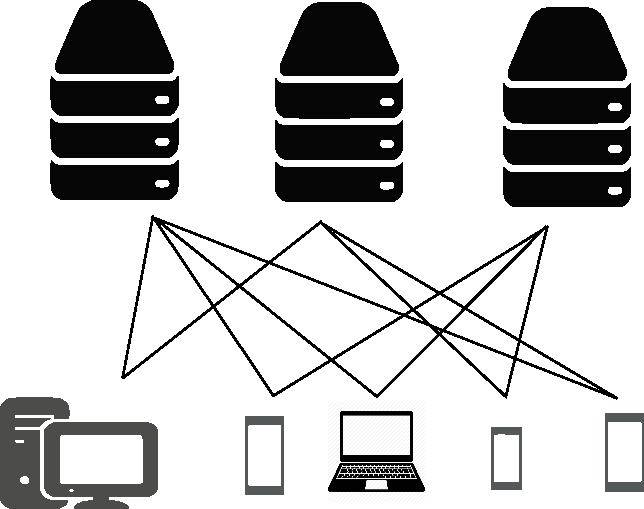
\includegraphics[width=0.6\linewidth]{server_sharing.pdf}
  \caption{An example server matching, one server is possible strategy of the client at the other end of the connecting line}
\label{server_sharing}
\end{figure}

Following the description in Section~\ref{congsetion_game}, we write the game for this problem, 
\begin{itemize}
\item The clients constitute the players in the game $\mathcal{N}$, and the collection of servers $\mathcal{M}$ is the strategy space for every player.
\item The cost of players in the game is equivalent to the latency for the clients .
If we denote the delay happens on the server as $d(n)$, where $n$ is the number of clients using the server, then the delay (cost) for a client (player) $i$ is $d(n_r(\sigma))$, where $n_r(\sigma)$ and $r\in \sigma_i$ is the number of clients using the server $r$.
\item As each user is allowed to use on server, this is a singleton congestion game according to Definition~\ref{background:singleton}.
\end{itemize}

Then, according to Theorem~\ref{background:finiteImprovement} and~\ref{background:polynomialConvergence}, after maximal $nm$ times best responses, the system reaches Nash equilibrium.
%More formally, this corresponding congestion game is composed of players (the self-interested clients) and resources (servers), where players are allowed to choose one certain resources to use. 
%There is cost (latency) generated on a resource for the players who use that resource, and the cost is monotonic increasing with the number of players using it. 
%As congestion game permits convergence when every players in turn adopt the strategy which leads to a better utility.



%Thus in server matching problem, when clients in turn choose a permissible server with a smaller predicted latency, then after finite number of steps, no client has motivation to switch any more, and we reach a NE.

%If every player greedily searches the allowed resources to decrease its cost, the dynamics will cease in Nash equilibrium, where no player has motivation to adopt a new set of resources unilaterally. 




\subsection{Variants of Congestion Game}
In the congestion game we have introduced in Section ~\ref{congsetion_game}, the cost caused on one resource is function of the number of players using that resource.
In some variants of congestion game, the cost is decided by some other factors.
In \textit{player specific congestion game}, different players may have different delay functions.
As to \textit{weighted congestion game}, different players may have different impacts on the delays of the resources they allocate, in other words, there is a weight for every player, and the congestion on a resource is the total weight of all players using that resource.

As to neither player specific congestion game nor weighted congestion game, the finite converge does not hold anymore.
But there exits NE for both of Player specific congestion game and weighted congestion game when they are singleton congestion game~\cite{Milchtaich1996111, FKKMS02}.
When these variant of congestion game are not singleton ones, \cite{Ackermann06purenash} points that NE exists when the strategy space of players are matroid.








\section{Optimization}

As discussed in Section~\ref{operation_model}, the available radio resources such as spectrum and transmission power are scarce, Meanwhile, new services raise new requirements for these resources.
Resource allocation and its optimization are needed to accommodate the needs.
Various optimization problems are formulated to improve radio resource usage in CRN~\cite{cacao_ca_2011, fuzzy_decision_09, resourceAllocation_imperfectSensing_2012}.
Optimization can be conducted from either a global view or from individual perspectives.

Many wireless resource allocation problems are formulated as constrained optimization problems.
Table~\ref{opt_table} shows the commonly used parameters, objectives and constraints of some optimization problems in wireless communication.
Part of the contents in Table~\ref{opt_table} refers \cite{Han:2008:RAW:1457343}.

\begin{table}
\begin{tabular}{|L{2.1cm}|C{3.8cm} | C{3.5cm} | C{3.7cm}|}
\hline 
 & Parametres & Optimization goals & Constraints \\ 
\hline 
Application layer & source-coding rate, buffer priority, packet arrival rate & minimal delay & base layer transmission, strict delay requirement \\ 
\hline 
Network layer & routing path & end to end delay/throughput & maximal hops, security concerns \\ 
\hline 
MAC layer & transmission frequency, transmission priorities & maximal overall throughput, minimal buffer overflow probability & contentions, time/frequency slot \\ 
\hline
Physical layer & transmission power, modulation, channel coding rate & minimal over power consumption, maximal throughput, minimal BER & maximal transmission power, caused interference on licensed users, available channel coding rate \\ 
\hline
\end{tabular} 
\caption{Optimization problem of cognitive radio networks}
\label{opt_table} 
\end{table}

The solutions to optimization problems can be categorized by their properties, \ie convex, linear, integer, or non-convex non-linear, etc.
In this thesis, we make use of different solvers, \ie Lindo, Gurobi, to solve the formulated optimization problems in different categories.


%Optimization outputs the results with the global information.
%Optimization is implemented on one entity, thus it is naturally suitable in centralized scheme.

\chapter{Congestion Game in Spectrum Allocation}
% Distributed Channel and Power Allocation in IEEE 802.22 Networks
\begin{quote}
{\textbf{Abstract}\\
\small In this chapter, we will see the application of congestion game in solving the channel allocation problem in the context of TV white space.
The channel allocation problem we will address is a general problem, as the transmission power is not identical for every transmitter and on each channel, actually, the transmission power could be unique for each transmitter-channel combination.
With the suitable utility function designed for transmitters, the behaviours of the transmitters can be described by a congestion game.
The algorithm of channel allocation is derived from the dynamics of the transmitter in the game, which reaches Nash equilibrium quickly.

Furthermore, we provide a complete solution to fully exploit TV white space complying with IEEE 802.22 standard.
We propose a centralized methods to regulate the upper bound of transmission power, so that to strictly protect the primary users.
%Proposed scheme also considers the necessity of distributable execution which decides the working channel and transmission power.
The the distributed channel allocation and power control are conducted sequentially.
%As to the channel allocation problem, we innovatively formulate this problem in to a canonical congestion game, and design efficient distributed channel selection strategy with the assistance of the centralized database.
%The successful practice of congestion game in this problem is enlightening for the application of congestion game in other problems where asymmetric interaction exists.
}
\end{quote}

\section{Introduction}



%%%%%%%%%%%%%%%%%%%%%%%%%%%%%%%%%%%%%%%%%%%%%%%%%%%%%

Secondary users working with TV white space is promising to cope with the scarcity of spectrum resources~\cite{FCC_2010_sedond_memorandumm}. 
Firstly, more unused TV white frequencies become vacant than ever with the ongoing transition from analog to digital broadcasts. Secondly, the frequencies of TV bands enable broadband access over larger geographic ranges compared to higher frequency bands. Nevertheless, services on TV receivers need to be protected with so called interference margin~\footnote{interference margin is the maximal interference caused by secondary users, which doesn't violate TV service.}~\cite{multipleIntf_pimrc11} which should not be exceeded by the accumulated interference caused by all secondary users working on the the channel.

\gls{FCC} and \gls{ECC} have announced rules on the transmission power of secondary users working in TV white space in US and Europe respectively~\cite{FCC_2010_sedond_memorandumm, ecc159}. 
FCC requires a minimum distance between secondary user and TV service area, besides, the transmission power for fixed secondary users is set as $4$ \textup{W}, which is a conservative setting. %If the interference margin of the TV receivers can be fully utilized, the requirement on secondary users' transmission power can be relaxed to some extent. 
FCC believes with these prudent measures, the interference margin can not be exceeded by interference from secondary users.
But it may not be the case when there are multiple secondary equipments transmitting at the same time, which is pointed in~\cite{Jaentti11}.
ECC requires the secondary users to adapt their maximum transmission power according to the distance away from the TV receivers.
%In this manner, secondary systems have to determine their maximum transmission power.

\begin{figure}[h!]
  \centering
  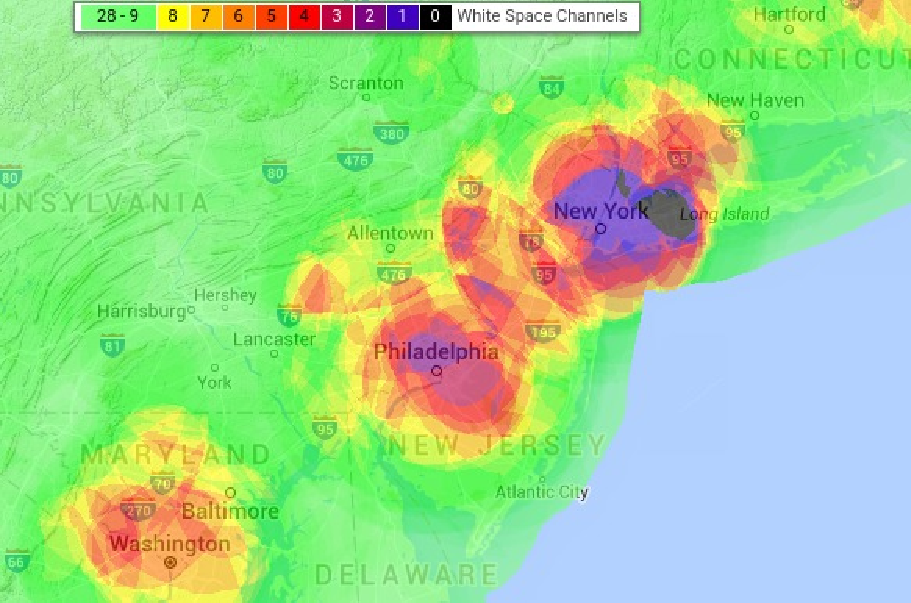
\includegraphics[width=0.9\linewidth]{TWWS_availability_east.pdf}
  \caption{Variability of available channels in a densely populated area. This figure is obtained from \cite{googleDatabase}}
\label{variability_avai_channel}
\end{figure}


FCC issued a memorandum~\cite{FCC_2010_sedond_memorandumm,FCCdatabasae} in 2010, which removes the mandatory rigid sensing requirements, and prompts the usage of geolocations\footnote{Geolocation means both geographic location and terrain.} of secondary users.
FCC regulates a centralized database, which registers all the secondary users within one certain area.
Secondary users can access the database, and can only use the channels assigned by the database.
% thus greatly facilitates the use of the spectrum with geolocation based channel allocation.
Work~\cite{SenseLess2011} follows this rule to obviate spectrum sensing and only relies on the database of TV incumbents to determine the white space availability for secondary users. 
The authors of~\cite{SenseLess2011} demonstrate the feasibility of predicting the available TV spectrum accurately using sophisticated propagation models (Longley-Rice) and geolocations of secondary users. 
A central database contains the geolocations of all TV stations, then the database calculates the received signal strength index (\gls{RSSI}) levels of TV \gls{UHF} signals on all secondary users and accordingly determines the available TV spectrum for them. 
If RSSI of a channel is below a certain threshold, TV service is regarded not to exist, and the channel is seen available there.
The calculated results on channel availability is very close to the measurement results.
The work of~\cite{SenseLess2011} gives big impetus to the usage of database mode.
%
%Through this work, it can be seen that the RSSI level caused by secondary users on TV receivers can be calculated accurately in a centralized entity if secondary users' transmission power, geographic location and appropriate propagation model are provided. 
As in TV white space, the accurate RSSI can be obtained with geolocations and suitable propagation model, given geolocation and appropriate propagation model, secondary users' maximum transmission power can be determined by the central entity according to the interference margin (maximum RSSI level from secondary users) on the TV receivers. 
%Obviously, transmission power control of secondary users has a significant impact on the performance of these systems. 

%To guarantee the protection on TV systems from harmful interference, FCC and IEEE propose a central database to regulate the access of TV spectrum by the secondary users.
%The centralized database registers the location and terrain information for all secondary users in the network, and decides the available channel and maximal permitted transmission power for each secondary user. 

%, and meanwhile the aggregated interference generated by them should be kept below a certain threshold on the TV system.

In this chapter, we investigate the usage of TV spectrum in a wireless regional area network which complies with IEEE 802.22 network.
The secondary users are assumed to be cellular base stations and associated terminals, all of which work on TV white spectrum. 
The base station is referred as WBS.
%The corresponding secondary base stations are referred as white base stations (WBS). 
Some cellular networks, \ie GSM or LTE network, work on licensed spectrum and emphasis on providing satisfactory services to their end terminals by choosing proper transmission channel and power. 
As to cellular network working on TV white spectrum, they have to keep one eye on the primary users to make sure that TV service is not violated, which makes the problem of channel and power selection difficult.
With the existence of central database, it is natural to utilize it as a central controller to assign channel and power usage for secondary users, but the secondary users may belong to different commercial groups and they may not contend with the assigned resource.
%Besides, as the TV channels have different quality, \ie interference level, and permitted transmission power, it is difficult for the database to assign them to the 
Hence, the spectrum sharing of the secondary users in IEEE 802.22 network should be decided in distributed manner and each secondary user takes care of its own interest, \ie to maximize its preferred utility.

Given all the other WBSs' selection on channel and transmission power, a WBS is interested in choosing the channel which brings it the best performance, \ie the data rate of its end users.
A WBS prefers to choose the channel which experiences the minimum interference, and the transmission power allowed on that channel is higher, so as to obtain better SINR on its terminals and meanwhile maximize their coverage \cite{wuinfocom09, HoangPowerChannel2010}. 
Nevertheless, high transmission power causes significant co-channel interference to other secondary users operating on the same channel. 
Hence, a secondary cell has to balance its transmission power and the caused interference on other cells, meanwhile to choose working channel to decrease the experienced interference on its terminals. 
The goal of this chapter is to protect the primary users from harmful interferences, meanwhile to find a strategy for WBSs to choose channel and power level in order to acquire good SINR on end terminals.

The rest of the chapter is organized as follows. we elucidate the system model in Section II, afterwards related work and problem formulation is presented in Section III. In Section IV, we discuss how to utilize the white space sufficiently by setting the transmission powers based on a convex problem formulation. We analyze the spectrum allocation problem under game theoretical framework and propose an algorithm in Section V, thereafter performance evaluation is presented in Section VI. Finally, we conclude our work and point out directions of future research in Section VII.


\section{System Model and Problem Statement}
\label{SystemModel}
Following the IEEE 802.22 standard, the primary systems considered in this chapter are digital TV (\gls{DTV}) stations which use the TV spectrum legally. 
TV stations provide service to passive TV receivers.
The secondary users are IEEE 802.22 Wireless Regional Area Network base stations utilizing the TV spectrum with senseless mode~\cite{SenseLess2011}. 
DTV's service should not be interfered by secondary systems. 
WBSs locate in one area which is surrounded by areas where TV service is delivered.
WBSs serve a set of end users/terminals.
These secondary systems are distributed over a certain area $A$ and is surrounded by multiple DTV service areas, as Fig.~\ref{sysmodel} shows. 
The set of DTV stations is denoted as $\mathcal{K}$ and the collection of WBSs is denoted as $\mathcal{N}$ where $|\mathcal{N}|=N$. 
The set of TV white spectrum contains multiple channels which are denoted as $\mathcal{C}$, they are assumed to be identical in terms of attenuation and shadowing on the same path.
Let $c(i)$ denote the channel used by a WBS $i\in \mathcal{N}$.

When two WBSs working on the same channel, co-channel interference is caused on each, while, neighbouring channel interference is not considered in our model. 
To simplify the analysis, we assume that each DTV station as well as each WBS utilizes exactly one channel.\footnote{The assumption that one WBS only utilizes one channel is for convenience of analysis. In reality multiple channel usage (channel bonding) is requisite as one single TV channel's bandwidth is 6 MHz which is not adequate for a WBS to fulfil system requirement. 
%We will relax this single channel usage assumption without hammering our scheme in the end of section \ref{sec_CA}.
}
We represent the usage of channel for WBS $i$ with a binary vector $X_i^{|\mathcal{C}|\times 1}=\{\cdots, x_{ik}, \cdots\}\in \{0,1\}^{|\mathcal{C}|}$, where $k\in \mathcal{C}$ and binary variable $x_{ik}$ denotes whether channel $k$ is used by user $i$. 
As each node can only uses one channel, for $X_i$, there is $\sum_{k=1}^{|\mathcal{C}|}x_{ik}=1$. 
The transmission power of WBS $i$ on channel $c$ is $P_i^c$. 


In the rest of the chapter, we use WBS and secondary base station interchangeably. 
There are interference measurement equipments deployed on the contours of TV service areas (as bold rectangles in Fig.~\ref{sysmodel}), which represent the worst located TV receivers in the TV service areas. 
For these interference measurement devices, an interference threshold should not be violated by the noise generated by the secondary users.
The deployment of the interference measurement devices is decided by the TV operators, which are usually along the contour of the area where TV receivers reside.
Thus, the locations of interference measurement devices vary according to the concrete location, geographic terrain and possible deployment of secondary networks. 
%For simplicity, we assume there is only one contour deployed for one TV area. % \todo{is contour 'clear' now?}.
WBSs are deemed to be static.
We assume the secondary base stations are not under the same operators, thus there is no scheduling mechanism available among WBSs.



\begin{figure}[h!]
  \centering
  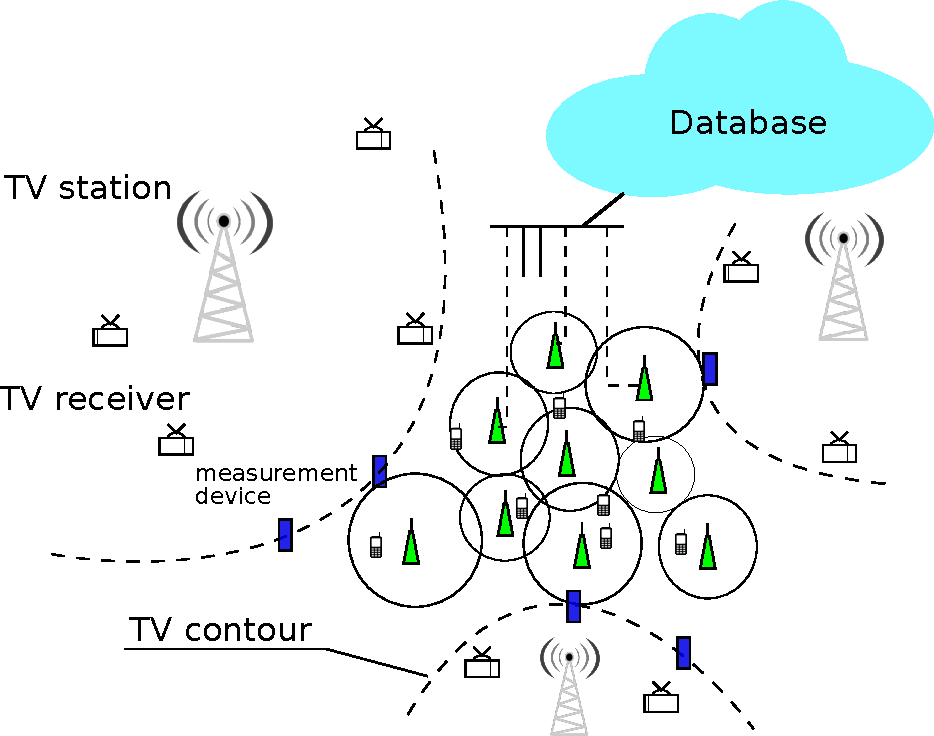
\includegraphics[width=0.9\linewidth]{systemmodel_working.pdf}
  \caption{System model: WBS cells and DTV systems}
\label{sysmodel}
\end{figure}

WBSs are interested in payload data communication with their associated terminals. 
As to performance metric for the \gls{QoS} provisioning, we choose the signal to noise and interference ratio (\gls{SINR}) on the terminals.
SINR is the ratio between the received power of signal of interest and the summed interference experienced by the terminal. 
%We only focus on the down-link SINR, as the interference caused by uplink communication is neglectable.
%
%Given a WBS $i$, another WBS which works on the same channel is denoted as $\bar{i}$.
As to a terminal $m$ associated to WBS $i$, the attenuation between its serving WBS $i$ and itself is denoted as $h_{im}$, and the attenuation between the interfering WBS $j$ and $m$ is denoted as $h_{jm}$.
The path loss is dependent on the distance between the corresponding equipments, e.g. $h_{im}=K \cdot d_{im}^{-\alpha}$, where $\alpha$ is the path loss exponent, $d_{im}$ is the distance between $i$ and $m$, $K$ is a constant which models the reference loss over a single unit of distance.  
$N_0$ denotes the thermal noise power.
Shadowing without fading is considered in our model.
$z_{im}$ models the zero-mean log-normally distributed shadow fading between $i$ and $m$, and the standard deviation is $\sigma_{\text{SH}}$.

The sum of all disturbing radio frequency effects (including interference) on terminal $m$ (we assume the working channel is $c$) is as following,
\begin{equation}
\label{interference}
\begin{aligned}
f_m^c=\sum_{\bar{i}} (P_{j}^c \cdot h_{jm} \cdot z_{jm}) +  N_0, \quad \quad j\in \mathcal{N}\setminus i, c(j) = c
\end{aligned}
\end{equation}
where $P_{j}^c$ denotes the transmission power of interfering WBS $j$.
%Note that $z$ is dependent on the individual transmitter/receiver pair, but we omit the subscripts for simplicity. 
The SINR on end terminal $m$ is,
\begin{equation}
\label{SINR}
\begin{aligned}
\gamma_{m} = \frac{P_{i}^c \cdot h_{im}\cdot z_{im}} {f_m^c}
\end{aligned}
\end{equation}



\subsection{Problem Statement}
Our goal is to design distributed solution for WBSs to choose channel and transmission power, so as to improve the SINR of their associated end terminals.
Each WBS's utility is a function of the SINR on all its end terminals, \ie the utility can be the average SINR at all its terminals.
When adopting a function of SINR on all terminals as utility, as the terminals are mobile and they are influenced by many factors, \ie the type of service provided to the terminals, the utility may diverge from the real performance of the terminals.
%Thus, due to the mobility of terminals, it is non realistic to adopt a function of SINR on all terminals.
On the other hand, it is not appropriate to choose one~\cite{spectrum_sharing_tvspace_2012} or more fixed terminals, and use their SINRs to represent the SINR for all the other terminals in that cell, because their location could diverge greatly with the locations of the other terminals.
Thus, we propose a metric \textit{QuasiSINR} to represent WBS's performance on providing services to its end terminals, which is independent on the actual locations of end terminals.

%We are interested in improving the SINR on the terminals of each cell by rendering WBSes to decide their channel and transmission power.
%The distribution of mobile terminals is varying and influenced by many factors, \ie the type of services provided to the terminals, the type of area and mobility of terminals.
%Thus when WBS decides its transmission parameter, it has to evaluate the SINR of all terminals.
%Furthermore, taking into consideration of terminals' SINR makes it very difficult to formulate WBS's preference on resources, \ie channel, power.
%Thus, we propose a simplified metric \textit{quasiSINR} for each WBS, which is independent on any terminals, and is able to  reflects the SINR on a circle around the WBS in a conservative manner.
%QuasiSINR can be easily adjusted by changing the radius of the circle so that the the circle goes through the majority of the terminal users.


\subsubsection*{QuasiSINR of WBS}

Instead of improving the SINR on each end users of WBSs, we propose a metric QuasiSINR to represent the services provided by WBSs to its end users.
Then the utility of WBS becomes a function of the  and try to improve this metric.
%QuasiSINR is an indication of SINR that a WBS can provide to its terminals.
QuasiSINR of a WBS is the ratio between the weakest signal of interest on a reference point and the summation of the strongest interference caused on the relevant reference point.

We need an auxiliary circle to construct the reference point for each WBS, which is shown in Figure~\ref{quasiSINRfigure}. % illustrates how is quasiSINR calculated.
As to WBS $i$, the auxiliary circle is the dashed circle centred at WBS $i$, whose radius is $\delta$.
Assume WBS $i$ and all the other WBSs work on the same channel $c$, then co-channel interference are caused on its end users by all the other WBSs.
The intersection of the auxiliary circle and the connecting line between WBS $i$ and one interfering WBS $j$, which is shown as red dot, is a reference point which corresponds to the interfering WBS $j$.
There are multiple reference points on the auxiliary circle, which corresponds to the co-channel interfering WBSs respectively.
The power of signal from $i$ on the auxiliary circle, the green dot, is the reference point for the power of signal of interest.
%The discussed WBS is denoted as $i$, and the rest WBSs are denoted as $j$, $j'$ and $j''$ respectively.
%We assume all the WBSs work on the channel $k$, this co-channel interference is caused on each WBS.
%An auxiliary dashed circle centering at WBS $i$ is shown, whose radius is $\delta$. 
We can see both of the reference point of interference and the reference point for the power of signal of interest are largely decided by the radius of the auxiliary circle $\delta$.

\begin{figure}[h!]
  \centering
  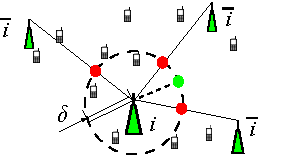
\includegraphics[width=0.6\linewidth]{quasiSINR2_2.pdf}
  \caption{QuasiSINR is the ratio between the power of signal of interest on the green point with the sum of co-channel interference on the red points}
\label{quasiSINRfigure}
\end{figure}


The co-channel interference on the reference point of WBS $i$ from WBS $j$ is,
\begin{equation}
\label{quasiSINR_inf}
\begin{aligned}
f_{ji}^c = P_{j}^c\cdot h_{ji}\cdot z_{ji} = P_{j}^c\cdot (d_{ji}-\delta)^{-\alpha}\cdot z_{ji}
\end{aligned}
\end{equation}
where $d_{ji}$ is the distance between WBS $i$ and $j$, while, $h_{ji}$ and $z_{ji}$ are the attenuation and shadowing from WBS $j$ to the relevant interference reference point.
The sum of interference on WBS $i$' interference reference points is denoted as $f_{i}^c$.
\begin{equation}
\label{quasiSINR_infs}
\begin{aligned}
f_{i}^c = \sum_{j\in\mathcal{N}, c(j)= c} f_{ji}^c
\end{aligned}
\end{equation}

The power of the signal of interest on auxiliary circle is expressed as,
\begin{equation}
\label{quasiSINR_1}
\begin{aligned}
\tilde{P_i}^c = P_i^c\cdot h_i\cdot z_i = P_i^c\cdot \delta^{-\alpha}\cdot z_i
\end{aligned}
\end{equation}
where $h_i$ and $z_i$ are the attenuation and shadowing from $i$ to any point on the auxiliary circle.


%In this model with flat environment, attenuation and shadow fading are function of distance, then we can say the power of signal caused by a WBS $j$ is the strongest co-channel interference caused by WBS $j$.
%In Figure~\ref{quasiSINRfigure}, $\tilde{f_{ji}}$ equals to received interfering power from WBS $j$ on the red dot, which is the crossing of the connecting line between WBS $i$ and $j$ and the auxiliary circle.


%In the rest of this chapter, $\tilde{P}$ and $\tilde{f}$ represent the received power of interest and the strongest interference on the auxiliary circle.
Then the quasiSINR of WBS $i$ is denoted as $\gamma_{i}$, 
\begin{equation}
\label{quasiSINR}
\begin{aligned}
 \gamma_{i} & = \frac{\tilde{P_i}^c}{f_i^c + N_0} \\
&=\frac{P_{i}^c \cdot h_i \cdot z_i} {\sum_{\tiny\substack{j\neq i, j\in \mathcal{N}\\c(j)=c(i)}} (P_j^c \cdot h_{ji} \cdot z_{ji}) + N_0}\\
&= \frac{P_{i}^c \cdot \delta^{-\alpha}\cdot z} {\sum_{\tiny\substack{j\neq i, j\in \mathcal{N}\\c(j)=c(i)}} (P_j^c \cdot (d_{ji}-\delta)^{-\alpha} \cdot z_{ji}) + N_0}
\end{aligned}
\end{equation}



%and we can see QuasiSINR is the ratio between the weakest signal of interest and the summation of the strongest interference.
The radius of the auxiliary circle $\delta$ can be adjusted to let WBS foster better service to the terminals in certain area.
For instance, to take care of the SINR on the border area of the cell, the radius $\delta$ can be set as the distance between WBS $i$ and the furthest associated terminal.
When the terminals concentrate towards to the WBS, $\delta$ can be set smaller to better fit to the terminals' distribution.
%but it can also be set by operator according to the base station's situation, such as the distribution of end terminals, and the geography of the coverage of the base station. 
%For this terminal furthest away, we now construct a worst-case SINR which factors in all interference from neighboring secondary cells as if they were closest to the considered terminal. Hence, QuasiSINR is the ratio between the weakest signal of interest and the summation of the biggest (possible) interference from other co-channel WBSs. 


%According to this construction, the weakest strength of the signal of interest is $P_i^c\cdot h_{iQ}\cdot z_{iQ} = P_i^c\cdot \delta^{-\alpha}\cdot z_{iQ}$ while the biggest possible interfering power from co-channel WBS $j$ is $P_j^c\cdot h_{jQ}\cdot z_{jQ} = P_j^c\cdot (d_{ji}-\delta)^{-\alpha}\cdot z_{jQ}$. We denote in this context by $Q$ the virtual worst-case terminal.
%%given at a position $Q$ (virtual measurement point) which is $\delta$ distance units away from the serving WBS, and $d_{ij}-e$ distance units away from any WBS $j$ \textit{at the same time}. The received power from WBS $i$ at this virtual measurement point is $P_i\cdot h_{iQ}\cdot z = P_i\cdot e^{-\alpha}\cdot z$, while the received interference power at $Q$ from any co-channel WBS $j$ is $P_j\cdot h_{jQ}\cdot z = P_j\cdot (d_{ji}-e)^{-\alpha}\cdot z$. 
%Hence, as we form the SINR such a virtual 'worst-case' terminal, the co-channel interference impact is overestimated as the total received interference power is given by the sum $\sum_{\forall j}P_j^c\cdot h_{jQ}\cdot z_{jQ}$ where index $j$ spans all co-channel WBSs with $i$. Formally, the QuasiSINR of WBS $i$ is given by:


%any change of the transmit powers of co-channel interference source (i.e. other WBS working on channel $k$) will have always fixed impact to the quasiSINR of the WBS concerned, 
Because of the auxiliary circle, the interaction between co-channel WBSs are independent on the location of individual end terminals, and WBSs only take care the co-channel WBSs. 
As a result,  the concrete terminals are excluded from the channel and power allocation problem, which simplifies the problem to be discussed. 
In the following part of this chapter, the notations are exclusively about the WBSs.
We clarify the meaning of some notations here.

\begin{table}[h]
\caption{Notations applied in the following part of this chapter}
\label{tab1}
\centering
\begin{tabular}{llr}
\toprule
%\multicolumn{2}{c}{Item} \\
%\cmidrule(r){1-2}
Symbol & Description \\
\midrule
$\gamma_i$ & QuasiSINR of WBS $i$\\
$f_{ji}^c$  & The interference caused by WBS $j$ on the interference reference \\
			& point of WBS $i$, and both of them work on channel $c$\\
$f_i^c$ & The sum of interference caused on the interference reference \\
			& points of WBS $i$ \\
$\tilde{P_i}^c$ & The power of the signal of interest on auxiliary circle of WBS $i$ \\
			& which works on channel $c$     \\
$P_i$		& The transmission power of WBS $i$\\
$h_{ij}$ & The attenuation from the co-channel interfering WBS $j$ to the \\
		& corresponding interference reference point of WBS $i$.\\
$h_{i}$ & The attenuation from the WBS $i$ to its auxiliary circle.\\
$z_{ij}$ & The shadowing from the co-channel interfering  WBS $j$ to the\\
		& corresponding interference reference point of WBS $i$.\\
$z_{i}$ & The shadowing from WBS $i$ to its auxiliary circle.\\		
\bottomrule
\end{tabular}
\end{table}

%Notice regrading the QuasiSINR, that any modification of the transmit powers of co-channel interference source (i.e. other WBS working on channel $c$) will have always the same scaled impact. I.e. we have symmetry among the co-channel interferes regarding their impact on the QuasiSINR. This is the main reason for introducing the QuasiSINR.\todo{?}



%\subsubsection*{Obtain quasiSINR and  Instead of Measurement}
Based on Formula~\ref{quasiSINR_infs}, as to WBS $i$, when the information is given, which include the locations of other co-channel WBSs, the radius of auxiliary circle and the standard deviation of shadow fading, then the co-channel inference caused on its interference reference points by other co-channel WBSs can be obtained, besides, WBS $i$ is also aware of the interference it causes on the interference reference points associated with other co-channel WBSs.


According to our system model, WBSs are able to access the central database which stores all WBSs' geolocations \ie working channel, transmission power, the characteristics of radio frequency environment such as parameters of attenuation and shadowing.
To obtain quasiSINR, one WBS doesn't need to measure the signal strength on the reference points which is needed in Formula~\ref{quasiSINR}, instead, it can can make use of the propagation model~\cite{Jaentti11} along with the operating parameters of all the other WBSs, which are stored in the central database to calculate the quasiSINR of any specific WBS.
%Besides, the channel usage of each WBS is also recorded in the data center.
%$h_{ij}$ and $z_{\bar{i}j}$, and also the transmission power of the interfering WBSs. 
%Thus when WBSes work in senseless mode, which can calculate the RSSI from one transmitter to an receiver with proper propagation model (e.g. Formula\ref{interference}\ref{SINR} can be calculated within database) with the geo-location and channel usage information. 
%A WBS also knows the interference it causes on the auxiliary circles of other co-channel WBSs via accessing the database.



\subsubsection*{Problem Formulation}
Our goal can be illustrated in the form of a constrained optimization problem.
To ensure fairness among WBSs, instead of maximizing the sum of quasiSINR of all WBSs, we minimize the sum of inverted quasiSINR. 
	\begin{equation}
\label{problem}
			\begin{aligned}
			& {\text{Minimize}}
			& & \sum_{i\in \mathcal{N}}\frac{1}{\gamma_{i}} \\
			& \text{subject to}
			& & \sum_{k=1}^{|\mathcal{C}|}x_{ik}=1 \\
			& & & P_{i,min}^c \leq P_i^c \leq P_{i,max}^c, c \in \mathcal{C}, i\in \mathcal{N}
			\end{aligned}
		\end{equation}
		where $P_{i,min}^c$ and $P_{i,max}^c$ are the minimal and maximal transmission power of the transmitter of WBS $i$, where are restricted by the hardware configuration or capabilities.
We assume $P_{i,min}^c$ and $P_{i,max}^c$ are identical for all WBSs and over all channels.

%XXX Please formalize the constraints, do not simply write 'one node, one channel'\todo{i'll do it!}
%where $\tilde{\gamma_{i}}$ is the QuasiSINR as defined in Equation~\ref{quasiSINR} XXX Always when you reference to a section, a figure, an equation or a table, mention the corresponding word in front of the reference - otherwise the reader does not know, should he reference to a section, an equation etc. - here I put in an 'Equation' for you but check this for the rest of the paper XXX. 
When a WBS works on different channels, the co-channel interference received by its end users from other WBSs is different.
In order to provide better service to its end users, WBS is motivated to choose the channel which either permits higher transmission power or experiences less interference, or the channel compromising the two factors according to Formula \ref{SINR}.
Achieving optimal white spectrum allocation in a distributed style is the goal of this work, furthermore, this distributed solution should converge fast and lead to an efficient and stable solution.


\section{Problem Decomposition and Related Works}
\label{decomposition_relatedwork}
In related works, the protection on primary users is taken care in the same time when channel and power selection are conducted.
But according to the current regulations and standards, there exist no communication means between the secondary users and the primary users.
Besides, when assuming such communication media is available and preventing primary users from being interfered during secondary users' power and channel allocation, the communication overhead between primary users and second users is considerable.

\subsection{Problem Decomposition}
We obtain the maximal transmission power over each channel for every WBS before dealing with channel and power allocation, afterwards, the transmission power should not exceed this power mask.
The maximal transmission power over all channels for each WBS is obtained at the centralized database.
As the database has the global info of both the secondary network and primary network, the attenuation and shadowing between any two users are known \ie attenuation is based on propagation model and shadowing is obtained from measurement, the database is able to guarantee the service of primary users not be interfered when all the WBSs work on the same channel.
Meanwhile, as the secondary users belong to different groups of interest, the channel and power allocation should be done in distributed manner.
%By decomposing the problem into two subproblems, the protection on the primary users from harmful interferences is excluded out of the latter consideration on channel and power allocation.

%We propose a distributed workaround for the join power channel allocation problem, so that 
In summery, we solve the channel and power allocation in downlink communication in IEEE 802.22 network by solving three sequential subproblems:
\begin{itemize}
\item  Firstly, given a set of secondary WBSs and their geo-locations, the maximum permitted transmission power on each channel for each WBS is determined, so that the interference margin of primary users can not be exceeded no matter how WBSs utilize the spectrum and power resources.
In other words, the dynamics in the secondary network is transparent to the primary system. 
\item Secondly, once the maximum permitted transmission power is determined, WBSs choose their operating channels.
Note that this channel assignment problem is different from the works available in literature, where the transmission power is identical over different channels for different WBSs.
In this subproblem, the maximum permitted transmission power $p_i^c$ could be different for different channel $c\in \mathcal{C}$ and different WBS $i\in \mathcal{N}$.
\item Thirdly, working with the maximal permitted transmission power may not be the optimal in terms of power consumption and the SINR on terminals, thus distributed power adjustment is conducted and the working channel is unchanged.
\end{itemize}
%The first subproblem is a centralized approach, the following two problems are solved with distributed schemes.
%We name the our solution of channel and power allocation as \gls{DiCAPS} (Distributed Channel Allocation and Power Selection).
The solution to the channel allocation subproblem is named as \gls{whiteCat} (white space Channel allocation).

In the following, we introduce the related works of spectrum and power allocation problem in CRN, especially the works about the usage of TV white space.
we also introduce the works related with subproblems mentioned above.

%We discuss the detailed problems in the following two subsections in combination with related work in the respective area.
%XXX Di, how can it be possible that we set the maximum transmit power and let the secondaries choose their operating channel afterwards? Isn't this related to each other ? XXX  
%XXX Answer: I decide the maximal transmission power in a very conservation way: let all of the WBSs work on the same channel and decide the max power. This need strong argument XXX

%In this paper we contribute by addressing this problem from two complementary directions. On the one hand, we study a convex formulation for setting the maximum transmit power at a set of secondary users given different interference margins for primary users. This scheme assumes a central controller to be in place which has geo-information and sufficiently detailed radio maps to characterize the path loss. We show that this convex formulation provides superior performance compared to linear problem formulations proposed in related work. Furthermore, we address the problem of assigning channels to WBS. Here, apart from the resulting cell performance, we also consider convergence of the assignment scheme as well as power consumption as important metrics. We propose a distributed scheme which interacts with a data base to get to know the channel choices of neighboring base stations, the interference relationships as predicted by radio maps as well as the maximal transmit powers. Formulated into a congestion game, the proposed schemes converges fast and provides superior performance in terms of cell performance and power consumption. 


\subsection{Resource Allocation in CRN}

We will emphasis more on the distributed solutions, but in order to give readers a full picture of the solutions as to resource allocation in CRN, we will also introduce the related works on centralized solutions.

Centralized solutions usually solve the formulated constrained optimization problems at a centralized unit.
In \cite{downlink-centralized-08-TWC}, the objective is to increase the number of supported terminals whose SINRs are above a threshold, and the constrains are to refrain the interference at the primary users within a certain margin.
Work \cite{joint_power_channel_linkpair_08ICT} minimizes the transmission power and meanwhile makes sure the SINR of terminal is above a threshold, but this work fails to consider the protection of primary users.
A heuristic algorithm is proposed in \cite{centralized_80222_sharing_ifip2011}, which considers the channel availability and transmission demand of each WBS.
%Spectrum allocation is solved after being formulated into a colouring problem.
The aforementioned two schemes don't consider varying the transmission power.
% xxxx important paper
%A centralized scheme is proposed in \cite{nashbargaining_2012jsac} for joint channel and power allocation among end terminals in OFDM cognitive radio network. 

There is a large variety of distributed solutions.
In order to avoid or to alleviate co-channel interference between cells, and to allow arbitrary number of cells to work in IEEE 802.22 network, \cite{Inter-Network_Spectrum_Sharing_80222_08} proposes distributed inter-network spectrum sharing scheme, where contention decisions are made in a distributed way and the winner cells can use the shared channels.
But this work doesn't consider the role of transmission power in the co-channel interference.
An distributed power allocation (single channel) scheme based on learning for secondary networks is given in \cite{aggregatedInf_Galindo_crowncom09}, where penalty function involving the interference threshold on primary systems is used.
%
\cite{HoangPowerChannel2010} discusses power control and channel assignment in both down-link and up-link communication in cellular network. 
Although the solution is distributed, primary users are required to cooperate with secondary base station in a learning process to decide the transmission power, in addition, there is only one secondary base station considered whereas we need to cope with the multiple cells in our problem.
%
Joint channel-power selection for multiple transmission links (pairs) is investigated in \cite{wuinfocom09}. 
The authors decompose the Lagrangian dual of the problem, then propose a distributed scheme based on the dual parameters. 
The scheme converges into pure Nash equilibrium, but in order to facilitate this scheme, monitors are required to watch interference from secondary users, moreover, monitors have to be equipped computational ability and interact with secondary users in the whole process of convergence.
%

As introduced in Chapter~\ref{INTRODUCTION}, game theory is a powerful tool in designing distributed algorithms.
A distributed joint power and channel allocation is proposed in~\cite{pimrc_2012}, each base station chooses optimal power level and channel to optimize its utility, which results in induced received interference and caused interference on primary users. 
The execution of this scheme is formulated into an exact potential game. 
For each base station, after several rounds of best responses in terms of channel and power level, Nash equilibrium is achieved.
There are some flaws hindering the application of this scheme.
Firstly, the paper doesn't provide means for base stations to obtain the needed information which is needed to calculate the utility function.
Secondly, it is not clear how to calculate the punishment in the utility function, which indicates whether and how much the interference threshold on primary users is violated.
Thirdly, the convergence speed of the scheme is not given, in fact, as the problem is formulated into a potential game, converge speed or the number of updates before convergence is a theoretic problem which is still unsolved.
Last but not least, as the utility function and the potential in the game are designed as the sum of received and introduced interference, the desired signal power and the punishment, the minimization of this \textit{sum} does indicate meaningful  performance metrics, \ie SINR on terminals, or the total transmission power consumption.
In~\cite{spectrum_sharing_tvspace_2012}, Chen et al. investigate the channel allocation problem in the scenario of TV white space.
The channel allocation problem is formulated into a potential game, individual WBS's utility is to maximize the capacity of one single static terminal.
%
Potential game is also adopted in work~\cite{tvws_paper_networking2015} to design algorithms, which mitigates the adjacent interference.
%
\cite{powerChannelAllocation_2015_shapley} adopts cooperation game to research the coexistence of femtocells.
Each femtocell negotiates with neighbouring fremcells, and they form temporary coalition, but the goal of this solution is to allocate resource block in terms of time and transmission power.
\cite{joint_power_channel_linkpair_08ICT} proposes both centralized and decentralized solutions.
Two distributed schemes are proposed, joint channel and power allocation is formulated into a weighted potential game, as an alternative workaround, the problem is solved in two sequential phases.

%
Distributed algorithm based on Learning is proposed in \cite{cogCE_huang} for LTE to allocate the the resource block in down link, which leads to correlated equilibrium, but slow converge hinters its application.
%



\subsection{Utilization of TV White Space}
Here we introduce the solutions proposed on the utilization of TV white space, which includes regulations, proposed standards and recent research advances.
In accordance with the regulations of FCC, there are some prototype applications proposed in both cellular network~\cite{tvwhite_lte2011, multicell_geo_dyspan11} and WiFi-like network~\cite{whitefi09}.
The secondary users access a centralized data base to know the allowed channels and transmission power.
%
Standardization bodies are also working on TVWS utilization, including IEEE 802.22~\cite{802.22} for Wireless Regional Area Networks (\gls{WRAN}), IEEE 802.11af~\cite{802.11af} for WLAN, IEEE 802.15.4m~\cite{802.15.4m} for 802.15.4 wireless networks in TVWS and 802.19.1~\cite{802.19} for coexistence methods among local and Metropolitan Area Networks (\gls{MAN}).

%\cite{HoangPowerChannel2010} proposes a distributed solution for power control and channel assignment in both down-link and up-link communication in a WRAN, but the investigated secondary network is composed with only one base station and multiple terminals.

%% related work!!!
Scientific research on utilization of TVWS goes on in parallel with the regulatory agencies.
Feng et al.~\cite{hybridPricing_tvspace_2014} investigate the business model of TV spectrum utilization in database involved network structure, emphasis on the price policy of the channels approved by FCC.
Spectrum sharing in TVWS is formulated as a series of optimization problems. 
The guarantee that TV receivers should not be affected by the aggregate interferences form TVBDs is one constraint.
The objective can be maximizing TVBD's downlink transmission power~\cite{multipleIntf_pimrc11}, uplink transmission power~\cite{uplink_power_tvws13}, or best geographic distribution of TVBDs~\cite{withinTVcoverage_PIMRC13}.
A series of works~\cite{game_CA_association_ICDCS12,SA_CA_TVWS_2012crowncom, 802.22co-existence09, 802.22game_08globecom,self-coexistenceWRAN2010infocom} emphasise on interference mitigation among TVBDs via spectrum allocation.
Vehicular networks operating with TVWS assisted by TV database and cooperative sensing is discussed in~\cite{tvws_vtc13}.
Work~\cite{increaseTVWS12} steps further from the database paradigm and makes efforts to utilize the \textit{grey space}, where TVDB is allowed to operate even within the TV service area.

%After each update, WBS needs to access the data base to retrieve the current channel usage, then they can calculate xxx.



\subsubsection*{Related Works on Maximal Transmission Power Planning}
\label{MPowerPlanning}
%Secondary network should not interfere TV receivers, thus regulation on transmission power is necessary.
%\cite{Chen_PowerControl,SenhuaHuang10,Zhu09} propose schemes for secondary users to decide the transmission power with sensing technology, one prime consideration of schemes is obviating interfering incumbent primary users. A distributed scheme to adjust power based on learning is proposed in \cite{aggregatedInf_Galindo_crowncom09} for each WBS, where a penalty function involving the interference threshold is used. This scheme needs many steps to converge, and there is no interference margin for network dynamics.
%Solving the joint problem of power and channel allocation in a distributed manner is challenging.
  
To protect the TV receivers from harmful interference, the aggregate interference caused by WBSs at the contours of TV receivers should not exceed the interference margin.
Work \cite{maximum_power_TVWS_dyspan_2011} proposes detailed calculations which a geolocation database performs in order to derive location-specific maximum permitted EIRP levels for white-space devices (WSDs) which operate in digital terrestrial TV bands.
\cite{multipleIntf_pimrc11} considers the maximum permitted transmission power for the network which complies with IEEE 802.22 standard. 
The standard requires a centralized database to store the available channels for each secondary base station, thus centralized scheme can be conducted there after trivial modification.
The sufficient condition for the TV receivers not be interfered in the context of TV white space is formulated into a centralized linear programming program (\gls{LP}) in~\cite{multipleIntf_pimrc11}.
The objective function is to maximize the summation of all secondary base stations' transmission power, and the constraints are formed to satisfy the sufficient condition for every interference measuring device for the TV receivers. 
However, this approach doesn't take the channel assignment problem into account.
%XXX This discussion of the related work is a bit confusing. The problem is that it is no clear per discussed paper what the shortcoming of the approach is. I.e. you describe the approaches but you do not help the reader why this approach is not contributing to the goal defined in the first sentence. Try to reformulate this section more precisely expressing what is the problem with the corresponding approach XXX.



\subsubsection*{Related Works on Channel Allocation with Fixed Transmission Power Level}
\label{CA}
In our proposed solution, after obtaining the maximum transmission power on each channel, WBSs need to decide one channel to use, and the transmission power is the maximum transmission power, so as to mitigate interference among WBSs and provide the best SINR for their associated end users.
Note that in our problem, the transmission power is different for two interfering users when they work on the same channel.
%Here we assume WBSs' transmission power is the maximum permitted and fixed.

Channel allocation problem dealing with mitigating co-channel interference via channel allocation, which has been attracting plenty of research efforts in the past decade, from multiple channel mesh network~\cite{Hyacinth}, Ad hoc network~\cite{Ko_DistributedCA} up to cognitive radio network~\cite{SA_CA_TVWS_2012crowncom,qlearning_huang}. 
%which has been investigated in many scenarios.

Channel assignment problem tries to mitigate co-channel interference among users, which can be converted into colouring problem thus is NP hard~\cite{Hyacinth}. 
Authors of~\cite{Ko_DistributedCA} propose heuristic algorithms utilizing best response to improve its welfare, but the transmission power is assumed identical and path loss is deemed as symmetric, which renders this method problematic for our problem where transmission is non-identical and the path loss is asymmetric.
\cite{CApotentialLearning_05dyspan} formulates channel assignment problem in ad-hoc cognitive radio network into potential game which leads to pure NE, a learning scheme achieving slightly better performance is provided for comparison, but they assume the transmission power is identical and there is no noise in the secondary network, and the proposed random access mechanism demands a huge amount of information to be exchanged, which is a burden for network in ad-hoc structure.
\cite{CA_Felegyhazi_07infocom, Wu_GOP_CA_08infocom} investigate the channel allocation problem under game framework in same collision domain, the authors propose algorithms to converge to pure Nash equilibrium (NE) and strongly dominate strategy equilibrium respectively. 
%\cite{whitefi} discusses channel assignment in the domain of white space, while, it deals with the temporal and spatial existence of spectrum availability where AP and clients choose the same chunk of channels based on spectrum capacity, and leave the interaction among APs unconsidered.

Authors of~\cite{Ko_DistributedCA} propose heuristic algorithms utilizing best response based on the welfare on itself to assign channels among users.
Simulated annealing is applied to mitigate co-channel interferences in~\cite{SA_CA_TVWS_2012crowncom}.
For the same purpose, no-regret learning~\cite{qlearning_huang, hart00correlatedeq} is exploit to optimize the choice on channel.

All the available channel allocation schemes are designed under the same assumption, that the transmission power levels are identical, and the attenuation between any pair is reciprocal.
As to our knowledge, there is no work dealing with channel allocation problem where transmission power is different.
%XXX So here we have the same problem as above: Only for the first two papers you say explicitly what problems come up with them - for the rest you simply mention them and their approach. Here we really need a much more clearer formulation of the shortcomings - why are they failing to be a solution to our problem ? Furthermore, there seem to be quite a lot of work in game theory and power control in secondary networks - how do they relate to our work? XXX

%Channel allocation facilitates CRN to improve throughput~\cite{channelAllocation_throughput_12wcnc}, or cooperatively relay~\cite{channelAllocation_relay_2010ICASSP} and so on.
%This thesis emphasises on co-channel interference mitigation with distributed channel allocation. 



%In this work we concern the best possible quality-of-service provisioning by allocating channels on which fixed transmission power is used.
%In this paper we try to improve the SINR on secondary end terminals through WBSs' power-channel strategy. To facilitate analysis and proposition of solution, we propose a metric \textit{QuasiSINR} for each secondary base station to represent the SINR of the terminals in the coverage of that base station.


%\todo{todo:}
%\begin{itemize}
%\item what is the reason to design a distributed scheme for this problem.
%\begin{itemize}
%\item complexity (to w)
%\item overhead
%\item WBSs belong to different commercial organization (we actually propose a spectrum sharing paradigm)
%\end{itemize}
%
%\item argument 1: why is the utility used in the algorithm, in other words, what is the reason to chose it and what is the relation between it and the SINR on end users.
%
%\end{itemize}


%xxxxxxxxxxxxxxx
%%'tvws_paper_networking2015' needs reading.
%Scheduling Variable Rate Links via a Spectrum
%Server, centralized Spectrum Server that
%coordinates the transmissions of a group of links sharing a
%common spectrum.xxxxxx


\section{The Maximum Permitted Transmission Power}
\label{powermap}
%interference measuring devices
The WBSs work in underlay manner and coexist with primary TV stations and receivers, the aggregate generated interference from WBSs on each channel should not exceed the threshold of the TV receivers.
We adopt the interference model and the optimization methodology from the work of \cite{multipleIntf_pimrc11} to plan the maximum transmission power on each channel for WBSs.
%XXX Why is exactly this approach adopted ?XXX.
%\todo{describe\\ the\\ interference\\ model\\ of [14]} 
Having a global view of the propagation parameters, geolocations of WBSs and interference threshold at interference measuring devices which locate on the contour of TV service area, linear programming is implied in the database to calculate the maximum permitted power over each channel.

For WBS $i\in \mathcal{N}$, the maximum transmission power allowed on channel $c\in \mathcal{C}$ is denoted as $P_i^c$. 
As to each channel $c$, the generated interference on each interference measuring device should be within a predefined interference margin $I^c_{pt}$.
The interference margin in a slow fading environment is decided according to~\cite{aggregate_interference_shadow_fading_2010}.

Then the maximum permitted transmission power on channel $c$ for each WBS can be obtained by solving the following optimization problem,
	\begin{equation}
\label{lp}
		\begin{aligned}
		& {\text{Maximize}}
		& & \sum_{i\in \mathcal{N}} P^c_i \\
		& \text{subject to}
		& & \sum_{i\in \mathcal{N}} (P^c_i \cdot h_{i,pt}\cdot z) < I^c_{pt},\\
		& & & P_{min}^c \leq P_i^c \leq P_{max}^c		
		\end{aligned}
	\end{equation}
	
%	XXX I am wondering here: You already define the solution in this section rather than defining the problem as indicated in the section title - why do we need to introduce here the solution ?XXX

$P_{min}^c$ is the prudent transmission power. % by FCC, we set is as 4 W. 
$P_{max}^c$ is the maximum transmission power which is restricted by the hardware.
$z$ is shadow fading as introduced in \ref{SINR}.
Here we only consider the interference caused by WBSs, and omit the interferences from end terminals. 
Since WBSs' transmission power is higher and their altitude is higher\cite{multipleIntf_pimrc11}, the downlink transmission contributes the major part of interference\cite{infmitigate07mobicom}.
%, in contrary the interference caused by end terminals is trivial and omitted. 
The first constraint indicates that the interference margin will not be exceeded even when all the WBSs work on the same channel.


Formula~\ref{lp} will be solved for each channel $c\in \mathcal{C}$.
%There will be multiple constraints for \ref{cvx} if there are multiple DTV contours working on channel $c$. 
After solving the $|\mathcal{C}|$ problems, the maximum permitted transmission power vector $\bm{P^c} =\{P_1,\cdots,P_{|\mathcal{N}|}\}, \forall c\in \mathcal{C}$ is obtained.
%We solve this convex optimization problem with \cite{cvx} in the centralized base station.

When working with the same transmission power, the WBSs locating closer to the TV interference measuring devices contribute more to the aggregate interference comparing with the WBSs which locate far from the TV interference measuring devices.
Thus when implying linear programming to decide the maximal transmission power, the transmission power used by WBSs which are closer to the TV interference measuring devices is much higher than other WBSs.
As a result the maximum permitted transmission power on each channel obtained with LP is seriously unbalanced.

To address this fairness issue, we maximize the sum of the logarithmic value of every WBS's transmission power, and formulate the problem into a convex optimization problem.
	\begin{equation}
		\label{cvx}
		\begin{aligned}
		& {\text{Maximize}}
		& & \sum_{i\in \mathcal{N}} \log P^c_i \\
		& \text{subject to}
		& & \sum_{i\in \mathcal{N}} (P^c_i \cdot h_{i,pt}\cdot z) < I^c_{pt}, 
		\end{aligned}
	\end{equation}

This optimization will be solved for each channel $c\in \mathcal{C}$.

Figure~\ref{lpcvx} depicts the distribution of maximum permitted transmission power levels obtained in 100 simulations.
In each simulation the locations of TV interference measuring devices are randomly decided around the WBSs.
In Figure~\ref{lpcvx}, It shows that when applying optimization~\ref{lp}, WBSs' transmission power levels are either the minimum transmission power or the maximum power allowed by the equipment hardware.
When applying convex programming, the planed maximum permitted transmission power levels are distributed evenly in between the minimum and maximum power.
The gain of SINR on end terminals by applying convex optimization to decide the maximal transmission power is illustrated in the simulation section.

\begin{figure}[h!]
  \centering
  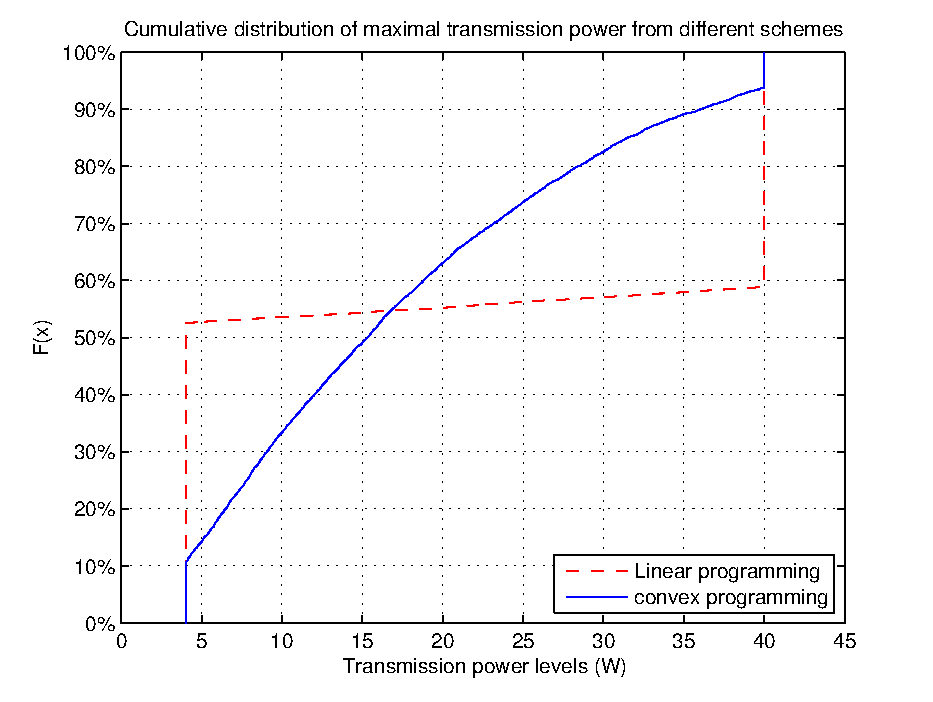
\includegraphics[width=0.89\linewidth]{lpcvxcdf100runs.pdf}
  \caption{Distribution of maximum permitted transmission power levels obtained from convex and linear programming formulations}
\label{lpcvx}
\end{figure}


Optimization problem \ref{cvx} provides the maximum permitted transmission power for each WBS and over each channel.
When all the WBSs working on the same channel, the generated interference doesn't exceed the threshold on the interference measurement devices at the contour of TV service area. 
If there are multiple channels available and WBSs are free to choose their preferred channels, the aggregate interference on one channel will be smaller than that when all WBSs work on that channel. 
Thus, there is exists a interference margin created by using multiple channels, which provides a room for network dynamics such as new WBS starting to work or increased interference on TV contour due to the variance of broadcast path condition. 
%XXX As mentioned above, it is not clear which impact the relationship between maximum transmit power planning and channel selection has XXX.


\section{Channel Allocation with Fixed Transmission Power}
\label{CA_fixedPower_2subproblem}
%As discussed in~\ref{CA}, there is 
First, we give the centralized solution to obtain the global optimum for this subproblem, then the decentralized scheme under the game theoretic framework is introduced.

\subsection{Centralized Optimization Programming}
\label{03_centralized_ca}
We formulate the channel allocation problem into a binary quadratic programming problem which can be solved in a centralized way.  
Let $X_i = \{x_{i1}\cdots x_{ik}\cdots x_{i|\mathcal{C}|}\}$ denote the vector of channel usage, there is $|X_i| = |\mathcal{C}|$ and binary element $x_{ik}$ represent whether WBS $i$ occupies channel $k$.
For two WBSs $i$ and $j$, there is,
\begin{equation}
\begin{split}
X_i^TX_j = \sum\limits_{k=1}^{|\mathcal{C}|}x_{ik}\cdot x_{jk} = 
\left\{ \begin{array}{ll}
1 & \mbox{if $c_i=c_j$} \\
0 & \mbox{if $c_i\neq c_j$} 
\end{array}
\right.
\end{split}
\end{equation}

The power levels across all channels are denoted by a constant vector $P^{|\mathcal{C}|\times 1}$, which is possibly nonidentical to WBSs due to different locations. 
The power used by user $i$ is $P_i^TX_i = \sum\limits_{k=1}^{|\mathcal{C}|}P_{i}^k\cdot x_{ik}$.


Problem \ref{problem} can be modeled via general purpose nonlinear optimization:
	\begin{equation}
\label{QLP}
		\begin{aligned}
		& \underset{}{\text{minimize}}
		& & \sum\limits^{n}_{i=1} \frac{\sum\limits_{j\in\mathcal{N}, j\neq i}P^TX_j(X_j^TX_i)h_{ji}z_{ji} + N_0}{P^TX_ih_iz_i}\\
		& \text{subject to}
		& & \sum\limits_{k=1}^{|\mathcal{C}|}x_{ik}=1, x_{ik}\in X_i\in \{0,1\}^{|\mathcal{C}|}\\
		\end{aligned}
	\end{equation}
Problem \ref{QLP} is a non-linear problem with binary variables, but it can be reformulated in to a quadratic programming problem as,
	\begin{equation}
\label{QLP_2}
			\begin{aligned}
			& \underset{}{\text{minimize}}
			& &	\sum\limits^{n}_{i=1} ( \sum\limits_{j\in\mathcal{N}, j\neq i}\sum\limits_k \frac{P_{jk}\cdot h_{ji}\cdot z_{ji}}{P_{ik}\cdot h_i\cdot z_i}\cdot  x_{jk}\cdot x_{ik}  + \sum\limits_k \frac{N_0}{P_{ik}\cdot h_i\cdot z_i}\cdot x_{ik})\\
			& \text{subject to} 
			& & \sum\limits_{k=1}^{|\mathcal{C}|}x_{ik}=1, x_{ik}\in X_i\in \{0,1\}^{|\mathcal{C}|}\\
			\end{aligned}
		\end{equation}

The reformulation is available in Appendix \ref{optdeviation}.
We use LINDO~\cite{lindo} which is a state of art non-linear problem solver to solve the problem, which employs Branch-And-Reduce method to get the global optimum for the problem. % We use the results obtained by solving this QLP problem as one reference in the coming section. 
The result of this centralized channel assignment will be evaluated in the simulation section with other schemes. 



\subsection{Distributed White Space Channel Allocation (WitheCat): Algorithm and Protocol}
\label{whitecat}
In this section a distributed scheme for WBSs to allocate channels is proposed, which is named as \underline{white} space \underline{c}hannel \underline{a}llocation \underline{t}echnology (WitheCat). 
WitheCat adopts the best response process, where each WBS (referred as $i$) chooses the channel which brings the bigger utility $u_i$ as the response of other WBSs' choices on channels.
%and the sum of all WBSs' utilities is minimized after finite times of updates even the interaction between WBSs are asymmetric. The utility is as follows,
WitheCat is depicted by algorithm \ref{whitecatalgo}.

\begin{equation}
\label{utility}
u_i =\dfrac{\sum\limits_{\tiny\substack{j\in \mathcal{N}, j\ne i,\\ c(\sigma_j)=c(\sigma_i)}}f_{ji}}{2\cdot \tilde{P_i}} + \dfrac{1}{2}\sum_{\tiny\substack{j\in \mathcal{N}, j\ne i,\\ c(\sigma_j)=c(\sigma_i)}}\dfrac{f_{ij}}{\tilde{P_j}} + \sum_{\tiny\substack{\mathcal{S}:i,j\in \mathcal{S},\\ c(\sigma_j)=c(\sigma_i)}}\dfrac{N_0}{C\cdot \tilde{P_i}}\\
\end{equation}

where $f_{ij}= P_i\cdot h_{ij}\cdot z$ and $f_{ji}= P_j\cdot h_{ij}\cdot z$.
Note that $f_{ij}$ is the sum of interference on WBS $i$'s interference reference points.
Overlooking the constant coefficient 2, the first item of $u_i$ is a part of the inverted QuasiSINR of station $i$. 
To minimize the first item, WBS $i$ needs to choose a channel either permits higher transmission power or experiences less interference, whereas the higher power increases the second item which is a part of inverted QuasiSINR of other co-channel WBSs. 
Hence, the cost function presents a reasonable comprise between the welfare of one WBS and others.

When WBS only emphasizes on its own utility (e.g. the first part of Formula~\ref{utility}), the best response process doesn't converge.
We have following theorem:
\begin{theorem}
\label{noconvergence}
\emph{With non-identical transmission power, if every WBS updates its channel based on Algorithm \ref{whitecatalgo} with utility based on its own interests, the process doesn't always converge.}
\end{theorem}
The proof is in Appendix \ref{proof}.


\begin{algorithm}[h]
\caption{Spectrum selection by WBS $i$}          % give the algorithm a caption
\label{whitecatalgo} 
\DontPrintSemicolon
\SetAlgoLined
\KwIn{the distance, path lose and shadowing parameter between WBS $i$ to WBS $j\in \mathcal{N}\setminus i$;\\  radius of auxiliary circle, noise $N_0$, total number of WBSs $N$;\\ for $j\in \mathcal{N}\setminus i$, the maximal transmission power $P_j^c, c\in \mathcal{C}$ and the working channel $c(j)$.
}
%\KwOut{a channel }

	\For{$c\in \mathcal{C}\setminus c(i)$}{
	 calculate $u_i(c)$ based on Formula \ref{utility}
	 \eIf{$u_i(c)<u_i(c(i))$}{
	 	$c(i)\leftarrow c$
	 }
	 {keep $c(i)$ unchanged}
	}
	
Notify database of its channel usage, which further notifies the other WBSs

\end{algorithm}



%//废话
%Imitating the player's behaviour in the congestion game, each base station tries to find the channel $c\in \mathcal{C}$ that brings the smallest $u_i$ based on the other stations' decisions, every channel update decreases the summation of utilities in the whole network and finally converges to a pure Nash equilibrium (proof is in section \ref{game}.


Some parameters needed to calculate the utility are identical for all WBSs, such as quasi distance $e$, the total number of WBSs $N$, number of channels $C$, attenuation factor $\alpha$, standard deviation $\sigma_{WBS}$ in flat shadowing and noise $N_0$, albeit the following information is further needed to calculate $u_i$: 
	\begin{itemize} %{labelitemi}{$\bullet$}
	\item $\sum_{\tiny\substack{j\in \mathcal{N}, j\ne i,\\ c(\sigma_j)=c(\sigma_i)}}f_{ji}^c, c\in \mathcal{C}$: the received interference on $i$' virtual measurement point from other WBSs $j$ working on the same channel for $\forall c\in \mathcal{C}$.
	\item $ f_{ij}^c$: the interference caused by $i$ on $j$'s virtual measurement point when $i$ works on channel $\forall c\in \mathcal{C}$.
	\item $P_j^c$: transmission power of $j$ for using $\forall c\in \mathcal{C}$.
	\end{itemize}
Unfortunately, it is difficult to get these interferences of interested measured, for station $i$, it is low efficient to scan all channels and obtain the interferences $f_{ji}$ on virtual measurement point for each channel, furthermore, it is impossible to split the interference $f_{ij}$ from the total interference received on WBS $j$' virtual measurement point. 

We refer \cite{CApotentialLearning_05dyspan} to decide the sequence for WBSs to update their channel. \cite{CApotentialLearning_05dyspan} proposes a method like random access mechanism of CSMA/DA, where the access for broadcast medium is changed to getting access to the centralized center to retrieve the current channel usage and update its new channel. All WBSs are able to access the database in one round (with random or predetermined sequence). As WBSs are connected with database, the control messages needed to decide the sequence will not become a burden. Update of channels can happen in the boot phase, or when the quality of services (the SINR on its end users) of WBSs falls below a threshold, or a fixed time duration comes to end, or a new WBS joins in the network. 

Similar with~\cite{SenseLess2011}, we let every WBS store the location information and maximal power map of all other WBSs, \ie $P_i^c, i\in\mathcal{N}, c\in\mathcal{C}$, and each WBS retrieves information about channel usage of other WBSs from centralized base station.
After executing Algorithm \ref{whitecatalgo}, it reports to centralized database of its channel if it updates the working channel.
As the location of WBSs and TV stations and the transmission channel and power of TV stations are usually static (entries of TV station change averagely once in 2 days\cite{SenseLess2011}), except for the channel usage in the network, the change of the other data stored in WBS is infrequent. 


\subsection{Analysis in Game Theoretical Framework}
\label{game}
In this section, We give the proof on whiteCat's convergence in the framework of congestion game theory.
Formulating a spectrum sharing problem into a congestion game and the concept of \textit{virtual resources} are firstly proposed in \cite{allerton08_liu}.
This work reversely engineers the distributed channel allocation schemes proposed in \cite{babadi_08, Ko_DistributedCA}, \ie unifies the algorithms with congestion game.
But the problem analysed in~\cite{allerton08_liu} assume the transmission power is identical, which is a major difference from the channel allocation problem discussed here. 

%\subsubsection{Congestion Game}
%A congestion game \cite{Rosenthal}\cite{Voecking06congestiongames} can be expressed by a tuple $\lambda=(\mathcal{N},\mathcal{R},(\sum_i)_{i \in \mathcal{N}},(g_r)_{r\in \mathcal{R}})$, where $\mathcal{N}=\left\{1,\ldots,N\right\}$ denotes the set of players (each each is labeled with a unique index number), $\mathcal{R}=\left\{1,\ldots,m\right\}$ the set of resources, $\Sigma_{i\in\mathcal{N}} \subseteq 2^{\mathcal{R}}$ is the strategy space of player $i$. Under strategy profile $\sigma=(\sigma_1,\sigma_2,\cdots \sigma_N)$, player $i$ chooses strategy $\sigma_i\in \Sigma_i$, and the total number of users using resource $r$ is $n_r(\sigma)=|\{i\mid r\in \sigma_i\}|$. The cost $g_r: \mathbb{N}\rightarrow \mathbb{Z}$ is a function of the number of users for resource $r$, $g_r^i=\sum_{r\in \sigma_i} g_r(n_r(\sigma))$. In our paper, $g_r^i$ is referred as \textit{congestion} and is Monotonic.
%
%Rosenthal's potential function $\phi:\sigma_1\times\sigma_2\times\cdots\times\sigma_n\rightarrow Z$ is defined as:
%\begin{equation}
%\label{4}
%\begin{split}
%G(\sigma) 
%& =\sum\limits^{}_{r\in \mathcal{R}} \sum\limits^{n_r(\sigma)}_{i=1} g_r(i)\\
%& =\sum\limits_{i\in \mathcal{N}} \sum\limits^{}_{r\in \sigma_i} g_r(n_r^i(\sigma))\\
%\end{split}
%\end{equation}
%$n_r^i(\sigma)$ means the number of players using resource $r$ and \textit{their indices are smaller than or equal to $i$}. Note that the potential is \textit{not} the sum of congestions experienced by every user. The change of the potential caused by one player's unilateral move from $\sigma$ to $\sigma'$ is equivalent to the change of gain (or loss) of that player.
%\begin{equation}
%\label{5}
%\varDelta G(\sigma_i \rightarrow \sigma_i') = g^i(\sigma_i',\sigma_{-i}) - g^i(\sigma_i,\sigma_{-i})
%\end{equation}
%$\sigma_{-i}$ is the strategy profile for all players except for $i$.
%As every congestion game is a potential game, and the total potential is finite, thus the number of improvements is upper-bounded by $2\cdot\sum\limits^{}_{r\in \mathcal{R}} \sum\limits^{n_r(\sigma)}_{i=1} g_r(i)$ \cite{Voecking06congestiongames}.
%
%
We have introduced congestion game in Chapter~\ref{background}, thus we only recap the essence of congestion game here.
In congestion game, each player acts selfishly and aims at choosing strategy $\sigma_i\in \Sigma_i$ to minimize their individual cost.
The gain (loss) caused by any player's unilateral move is exactly the same as the gain (loss) in the potential, which may be viewed as a global objective function.
For problems where the potential of the problem is the same with the summation of the cost of all users, the cost function can be used as a utility function directly.
This equivalence doesn't exist in our problem, but by carefully choosing the cost function for players, we can make sure that the change of individuals' cost is in the same direction with that of the global utility.



\subsubsection*{The Congestion Game Formulated from the Algorithm WhiteCat}
\label{gameforproblem}
We utilize the conception of virtual resource which is firstly introduced in \cite{allerton08_liu}. 
Virtual resource is a triplet $\{i, j, c\}$, where $i,j$ are two WBSs and $c\in \mathcal{C}$ is one channel.
This piece of resource is regarded used by $i$ when both $i$ and $j$ use channel $c$, otherwise, $\{i, j, c\}$ is not used by any WBS.

In the following, we list the element of the congestion game which emulates Algorithm~\ref{whitecatalgo}.
In this section, player and base station are used interchangeably.

\begin{itemize}
\item Player $i$' strategy space is $\Sigma_i=\{(i,j,c), j\in \mathcal{N}, j\ne i, c(\sigma_j)=c, c=1,2,\cdots,N\}$, and $i$ has $C$ admissible strategies, one strategy related with channel $c\in\mathcal{C}$ is described by the set of virtual resources it uses: $\sigma_i=\{(i,j,c), j\in \mathcal{N}, j\ne i, c(\sigma_j)=c\}$, note that virtual resource $(i,j,c)\neq(j,i,c)$.

\item Under the strategy profile $\sigma=(\sigma_1, \sigma_2, \cdots \sigma_N)$, player $i$ obtains a total cost of 

	\begin{equation}
\label{6}
		\begin{split}
		g^i(\sigma)=
		& \sum\limits^{}_{\tiny\substack{j\in \mathcal{N},j\neq i,\\ c=c(\sigma_i)=c(\sigma_j)}} (g_{(i,j,c)}(n_{(i,j,c)}(\sigma))+g_{(j,i,c)}(n_{(j,i,c)}(\sigma))
		\end{split}
		\end{equation}
\end{itemize}

The transmission power over all channels of player $i$ is $\{p_i^1, p_i^2,\cdots, p_i^{|\mathcal{C}|}\}$.
%According to our system model, interfere xxxxxx
%Path loss is assumed reciprocal: $h_{ij}=h_{ji}$, but nor is the flat fading $z$. To keep the formula clear in the following part, we denote $\tilde{f_{ij}}= P_i\cdot h_{ij}\cdot z$, $\tilde{f_{ji}}= P_j\cdot h_{ij}\cdot z$, $\tilde{P_i}=h_{iQ}$ for $i\in \mathcal{N}$, where $h_{ji}=h_{ij}=(d_{ji}-e)^{-\alpha}, h_{ii}=h_{jj}=e^{-\alpha}$, $d_{ji}$ is the distance between base station $i$ and $j$, and $\delta$ is the quasi distance introduced in section \ref{SystemModel}. $N_0$ is noise which is identical for any channel and any WBS. 
We define the cost function for virtual recourses $(i,j,c)$ as follows,
\begin{equation}
\label{costfuc4resrc}
\begin{split}
g_{(i,j,c)}(k) = 
\left\{ \begin{array}{ll}
%\tilde{f_{ji}}/(2\tilde{P_i}) + f_{ij}/(2\tilde{P_j}) + N_0/(C\cdot \tilde{P_i})\\\\
%=\dfrac{P_j\cdot h_{ji}\cdot z/2 + N_0/C}{P_i\cdot h_{iQ}\cdot z} +\dfrac{P_i\cdot h_{ij}\cdot z/2}{P_j\cdot h_{jQ}\cdot z} & \mbox{if $k=2$} \\
\dfrac{f_{ji}}{2\tilde{P_i}} + \dfrac{f_{ij}}{2\tilde{P_j}} + \dfrac{C\cdot N_0}{N\cdot \tilde{P_i}} & \mbox{if $k=2$} \\
%=\dfrac{P_j\cdot h_{ji}\cdot z/2 + N_0/C}{P_i\cdot h_{iQ}\cdot z} +\dfrac{P_i\cdot h_{ij}\cdot z/2}{P_j\cdot h_{jQ}\cdot z} & \mbox{if $k=2$} \\
0 & \mbox{otherwise}
\end{array}
\right.
\end{split}
\end{equation}


As resource $(i,j,c)$ only lies in the strategy space of player $i$ and $j$, thus can only be accessed by this two players.
More specifically, according to Formula~\ref{costfuc4resrc}, the cost of resource $(i,j,c)$ is only decided by the number of players using it, which is either 0 or 2.
At the first glance, this is a player specific congestion game, as $g_{(i,j,c)}$ is decided by the relevant players' transmission power and inference.
But actually the resource ${(i,j,c)}$ excludes the players except for $i$ and $j$ from using it, thus the cost happened on this resource is only dependant on how many of players from the set $\{i, j\}$ to use it.
Hence, the cost is a function of the number of players using the resource, and this is a canonical congestion game.

\subsubsection*{Bridging the Game and Algorithm WhiteCat}

When we substitute Formula \ref{costfuc4resrc} to Formula \ref{6}, the total cost for user $i$ under strategy profile $\sigma$ . 

\begin{equation}
\label{cost1player}
\begin{split}
g^i(\sigma)
%& = \sum_{\tiny\substack{j\in \mathcal{N}\setminus i,\\ c=c(\sigma_j)=c(\sigma_i)}} g_{(i,j,c)}(2) + \sum_{\tiny\substack{j\in \mathcal{N}, j\ne i,\\ c=c(\sigma_j)=c(\sigma_i)}} g_{(j,i,c)}(2)\\
& = \sum_{\tiny\substack{j\in \mathcal{N}\setminus i,\\ c=c(\sigma_j)=c(\sigma_i)}} (g_{(i,j,c)}(2) + g_{(j,i,c)}(2))\\
%& = \sum_{\tiny\substack{j\in \mathcal{N}, j\ne i,\\ c(\sigma_j)=c(\sigma_i)}} (\dfrac{f_{ji}/2 + N_0/C}{\tilde{P_i}} + \dfrac{f_{ij}/2}{\tilde{P_j}})\\
& = \sum_{\tiny\substack{j\in \mathcal{N}\setminus i,\\ c(\sigma_j)=c(\sigma_i)}}(\dfrac{f_{ji}}{\tilde{P_i}} + \dfrac{f_{ij}}{\tilde{P_j}}+ \dfrac{C\cdot N_0}{N}(\dfrac{1}{\tilde P_i}+\dfrac{1}{\tilde P_j})) \\
& = \dfrac{\sum\limits_{\tiny\substack{j\in \mathcal{N}\setminus i,\\ c(\sigma_j)=c(\sigma_i)}}f_{ji}}{ \tilde{P_i}} + \sum_{\tiny\substack{j\in \mathcal{N}\setminus i, \\c(\sigma_j)=c(\sigma_i)}}\dfrac{f_{ij}}{\tilde{P_j}} + \dfrac{CN_0}{N}\sum_{\tiny\substack{j\in \mathcal{N}\setminus i,\\ c(\sigma_j)=c(\sigma_i)}}(\dfrac{1}{\tilde{P_i}}+\dfrac{1}{\tilde{P_j}})\\
& = \dfrac{\sum\limits_{\tiny\substack{j\in \mathcal{N}\setminus i,\\ c(\sigma_j)=c(\sigma_i)}}f_{ji}}{ \tilde{P_i}} + \sum_{\tiny\substack{j\in \mathcal{N}\setminus i,\\ c(\sigma_j)=c(\sigma_i)}}\dfrac{f_{ij}}{\tilde{P_j}} + \dfrac{2CN_0}{N}\sum_{\tiny\substack{i\in\mathcal{S}\subset\mathcal{N},\\\mathcal{S}:\forall i\in \mathcal{S}\\ c(\sigma_i)=c}}\dfrac{1}{\tilde{P_i}}\\
\end{split}
\end{equation}

where $\mathcal{S}$ denotes the set of WBSs whose working channel is the same with WBS $i$.

Now we are going to have a look at the \textit{potential} of the network.
According to the expression of Rosenthal's potential in Formula~\ref{2:Rosenthal_potential_newdelay}, the potential is accumulated by adding the players' cost sequentially, in particular, the value which is added is the cost that player experiences when it starts to use the relevant resource, and the value is not changed when other players come to use that resource.
Back to our problem, for two WBSs $i,j\in \mathcal{S}$, we assume WBS $i$'s index is smaller than $j$'s index, then the potential increased by $i$ using the resource $\{i,j,c\}$ is 0 according to Formula~\ref{6}, and the increase brought in by $j$ using the resource $\{i,j,c\}$ is $g_{(i,j,c)}(2)+g_{(j,i,c)}(2)$. 
In other words, for each interfering pair of WBSs, only the WBS with bigger index contributes to the potential. 
Then the total potential is, 
\begin{equation}
\label{allPotential}
\begin{split}	
G(\sigma) 
& =\sum\limits^{}_{r\in \mathcal{R}} \sum\limits^{n_r(\sigma)}_{i=1} g_r(i)  =\sum\limits_{i\in \mathcal{N}} \sum\limits^{}_{r\in \sigma_i} g_r(n_r^i(\sigma))\\
%& = \sum\limits_{i\in \mathcal{N}}\dfrac{\sum\limits_{\tiny\substack{j\in \mathcal{N}, j\ne i,\\ c(\sigma_j)=c(\sigma_i)}}\tilde{f_{ji}}}{\tilde{P_i}} + \sum\limits_{\tiny\substack{\mathcal{S}\backepsilon i, \mathcal{S}\subset \mathcal{N},\\ \forall j\in \mathcal{S}, j\neq i,\\ c(\sigma_j)=c(\sigma_i)}}  (\dfrac{\mid\mathcal{S}\setminus 1 \mid}{C} \frac{N_0}{\tilde{P_i}})
& = \sum\limits_{i\in \mathcal{N}}\dfrac{\sum\limits_{\tiny\substack{j\in \mathcal{N}, j\ne i,\\ c(\sigma_j)=c(\sigma_i)}}f_{ji}}{\tilde{P_i}} + \dfrac{CN_0}{N}\sum\limits_{\tiny\substack{\mathcal{S}\subset \mathcal{N},\\ \forall i\in \mathcal{S}, c(\sigma_i)=c}} \mid \mathcal{S}\mid   \sum\limits_{\tiny\substack{i\in \mathcal{S}}}\frac{1}{\tilde{P_i}}
\end{split}
\end{equation}

 note that the summation of one WBS's congestion is related to its index. 

%Question:
%
%When power is variable, is it still a congestion game, or potential game?

When players minimize their utilities (cost or potential) illustrated by Formula \ref{cost1player}, the total congestion in the secondary network given by Formula \ref{allPotential} decreases monotonically before reaching one Nash equilibrium. Players' greedy update in the game to minimize its cost Function\ref{cost1player}, which ceases finally in pure Nash Equilibrium. The strategy and cost function of players in the game is transplanted as Algorithm \ref{whitecatalgo} and utility Function \ref{utility} respectively.


\subsubsection*{Gap between the Potential of Game and the Objective}
It is natural to raise the question, is the sum of the final utilities of all WBSs exactly the same with the value of potential when the game converges to a Nash equilibrium, which is represented by \ref{allPotential}?
The answer is, they are identical when $N_0$ is zero, and there will be a little difference when $N_0$ is not zero.
Recall the target objective we want to minimize in Problem \ref{problem} is,
\begin{equation}
\label{compare}
\begin{split}	
\sum_{i\in \mathcal{N}}\dfrac{f_i}{\tilde{P_i}}
& = \sum\limits_{i\in \mathcal{N}}\dfrac{\sum_{\tiny\substack{j\in \mathcal{N}, j\ne i,\\ c(\sigma_j)=c(\sigma_i)}}f_{ji}+N_0}{\tilde{P_i}}\\
& = \sum\limits_{i\in \mathcal{N}}\dfrac{\sum_{\tiny\substack{j\in \mathcal{N}, j\ne i,\\ c(\sigma_j)=c(\sigma_i)}}f_{ji}}{\tilde{P_i}} + \sum\limits_{i\in \mathcal{N}}  (\dfrac{N_0}{\tilde{P_i}})\\
\end{split}
\end{equation}
We notice that only the last items of the objective~\ref{compare} and the potential of the congestion game~\ref{allPotential} are different.
When $N_0=0$, the potential is exactly the same with the object we want to minimize.
When $N_0\neq 0$, if channels are evenly distributed and there is $C/N*\mid \mathcal{S}\mid = 1$, then Formula~\ref{compare} and \ref{allPotential} are also the same.
In both cases, the sum of utilities \ref{compare} decreases monotonically with every update of WBSs before the system reaches Nash Equilibrium.
%
When $N_0\neq 0$ and Formula~\ref{compare} and \ref{allPotential} are thus different, the monotonicity on the decrease of sum of utilities \ref{compare} is not perceived, whereas the system will still cease to NE.

Based on above analysis, we can see the assumption that each WBS only occupies one channel can be easily removed.
If we regard one WBS as multiple ones which locate at the same place, and each WBS works on one distinct channel, then the proof on convergence of whiteCat can be applied directly to this case.

Note that the convergence of the game is independent on the the concrete form of the cost function. 
We adopt the function \ref{cost1player} to let the potential of the game be the same with the total utility of all WBSs, so that by executing Algorithm~\ref{whitecatalgo}, the system objective experiences a monotonic decreasing process before the system reaching NE.
The algorithm has potential to solve many other problems, where one user's decision affects others.
In this case, the utility of one user can be formulated to incorporate the information of its own utility and others', then the congestion game theory can be used to analogize.
%Hence, WhiteCat scheme provides a prototype for the problems where the interaction among users are asymmetric.



\subsubsection*{Communication Overhead of WhiteCat}

The problem of channel allocation with different and fixed transmission power is NP hard.
WhiteCat is a distributed scheme but certain information of the other WBSs is needed.
The centralized base station is piggybacked to provided the needed information.
As to one WBS, the number of such inquiries is the number of steps before convergence.

In our formulated congestion game, a player $i$ is allowed to access up to $(N-1)$ resources in the same time, \ie $\{i, j_1, c(i)\}, \{i, j_2, c(i)\} \cdots \{i, j_{N-1}, c(i)\}$, thus the upper bound of converge steps can not be obtained from the conclusion~\ref{2:Rosenthal_potential_newdelay} for singleton congestion game.
But our problem is special because for each resource, the possible number of players allowed to use each resource is either 2 or 0.
Thus we can refer the method used in Section~\ref{singleton_congestion_game} to analyse the update times for our problem.
Firstly, we sort the cost values in increasing order.
Although a WBS 
\begin{equation}
\label{2:Rosenthal_potential_newdelay}
\begin{split}
\phi(\sigma) 
& =\sum\limits^{}_{r\in \mathcal{R}} \sum\limits^{n_r(\sigma)}_{i=1} g_r(i)\\
& \leq \sum\limits^{}_{r\in \mathcal{R}} \sum\limits^{n_r(\sigma)}_{i=1} n\\
& \leq n^2m
\end{split}
\end{equation}

The upper bound of total update steps is $2n^2$, thus averagely, the upper bound of update steps for each WBS is $2n$.



\section{Variable Transmission Power After Channel Allocation}
\label{powerAllocation}
After deciding on the working channel, WBSs operate with the maximum permitted transmission power.
As the utility defined in Formula~\ref{quasiSINR} is a division of linear function of transmission power and received interference, it is natural to assume that there could exist a vector of transmission power $\{p_1, p_2, \cdots, p_N\}$ where $p_i<P_{max}^c,\forall i\in \mathcal{N}$, and the performance doesn't diverge much from the already achieved performance.
When using the same utility as Formula~\ref{quasiSINR}, there is no WBS having the motivation to diverge from the power level (the maximum permitted power) if the other WBSs keep their transmission power unchanged.

We adopt the utility proposed in~\cite{power_control_utility_98} as our utility function.

\[u= \dfrac{E\cdot R}{p}(1-e^{-0.5\cdot \gamma})^L\]

This new utility is function of both its own transmission power and quasiSINR, thus one WBS doesn't need relevant information from other WBSs. 
This function has several attracting properties.
It is a monotonically increasing function of $\gamma$ for a fixed transmission power $p$.
It approaches to 0 when $\gamma$ increases to infinity, and it is a monotonically decreasing of the transmission power $p$ for a fixed $\gamma$.
This function goes to 0 when $p$ goes to either 0 or infinity.
To adopt this algorithm, every WBS keeps on minimizing its utility and finally all the WBSs achieve Nash equilibrium.
 


%base start to adjust their transmission power in a decentralized manner.
%The problem becomes a traditional power control problem: find a power level to maximize (or minimize) a proposed utility which is function of transmission power and SINR.
%We utilize a convex function as utility, and there exists $\textit{P}$ that WBSs are in NE.

%\textcolor{brown}{What we need to do is to find a vector of transmission power $\{p_1, p_2, \cdots, p_N\}$ in NE state,} where each element is the power level of one WBS. 
%Needless to say, there will be $p_i \leq P_i^c$ where $P_i^c$ is the maximal permitted transmission power on channel $c$ at WBS $i$.
%If there is $p_i = P_i^c$ for any $i$, we don't need to vary transmission power after the channel allocation -- at least told by theory.



\section{Joint Channel and Power Allocation}
In the section~\ref{CA_fixedPower_2subproblem}, the problem is decomposed into three subproblems which are solved sequentially.
The first is solved with linear/convex programming in the centralized database, and the others are solved with distributed schemes.
The decomposition of the original problem, and the distributed scheme may yield result which is far away from the global optimum, so in this section, we propose a centralized scheme which looks for the global optimum in order to examine the performance of our cascaded and distributed channel and power allocation scheme.


\subsection{Centralized Optimization}
\label{opt_channelAndPower}
When we consider to optimize the transmission power and channel jointly, the optimization problem \ref{QLP_2} is not quadratic any more and becomes mixed integer non-linear problem, for which no efficient solution exists.
We reformulate problem \ref{QLP_2} into a mixed binary quadratic optimization problem with some auxiliary variables created, \ie binary number $\alpha$, real number $\beta$ and $q$, where
	\begin{equation}
	\label{alpha_opt}
x_{jk}\cdot x_{ik} =\alpha_{ij}^k
	\end{equation}
	\begin{equation}
	\label{beta_opt}
\beta_{ij}^k = p_j^k\cdot \alpha_{ij}^k
	\end{equation}
	\begin{equation}
	\label{q_opt}	
\frac{1}{p_i^k} = q_i^k
	\end{equation}
Then the optimization problem can be stated as:
	\begin{equation}
\label{midp}
			\begin{aligned}
			& \underset{}{\text{minimize}}\\
			&\sum\limits^{n}_{i=1}(\sum\limits_{j\in\mathcal{N}, j\neq i}\sum\limits_k q_{i}^k\cdot \beta_{ij}^k \cdot h_{ji}\cdot z + \sum\limits_k N_0\cdot q_{i}^k\cdot x_{ik})\\
			& \text{subject to:} \\
			& x_{jk} + x_{ik} - \alpha_{ij}^k\leq 1 \\
			& -x_{jk} - x_{ik} +2\cdot \alpha_{ij}^k \leq 0 \\
			& \beta_{ij}^k - p_j^{k,max}\cdot \alpha_{ij}^k \leq 0 \\
			& - \beta_{ij}^k + p_j^{k,min}\cdot \alpha_{ij}^k \leq 0 \\
			& \beta_{ij}^k - p_j^k - p_j^{k,min}\cdot \alpha_{ij}^k \leq -p_j^{k,min} \\			
			& -\beta_{ij}^k + p_j^k + p_j^{k,max}\cdot \alpha_{ij}^k \leq p_j^{k,max} \\			
			& \sum\limits_{k=1}^{|\mathcal{C}|}x_{ik}=1, x_{ik}\in X_i\in \{0,1\}^{|\mathcal{C}|}\\
			& q_i\cdot p_i =1\\
			\end{aligned}
		\end{equation}
%		\todo{result is not ready.}

The objective function is quadratic.
We notice that all the constraints except for the last one are linear.
The first two constrains realizes Formula~\ref{alpha_opt}, the following four constraints realizes Formula~\ref{beta_opt}.
Due to the quadratic equability constraint $q_i\cdot p_i =1$, the optimization problem is non-convex which makes this optimization problem very challenging to solve~\cite{hmam2010quadratic,Quadratic_min_one_equality}.
%
Linearisation is possible when the matrix Q in the quadratic is positive definite.% 'Quadratic Optimisation with One Quadratic Equality Constraint'.
As we don't regulate the locations of the WBSs, and the attenuation is random among them, thus the positive definite can not be guaranteed.
We use solver LINDO~\cite{lindo} to look for the global optimum.




%One workaround to avoid global searching is to linearise the equality constraint. 
%After linearising constraint $q_i\cdot p_i =1$, the problem becomes mixed integer quadratic problem, and can be solved with Gurobi.


\section{Performance Evaluation}
\label{simulation}
Performance evaluation consists two parts, in the first part whiteCat are compared with other distributed schemes proposed for the problem of channel allocation with different fixed transmission power, where the transmission power levels associated with WBSs and channels are different.
In the second part, we compare the distributed joint channel and power allocation solution with other solutions for this problem.
To illustrate the structure, we list the contents in Figure~\ref{evaluationContent}.

\begin{figure}[h!]
  \centering
  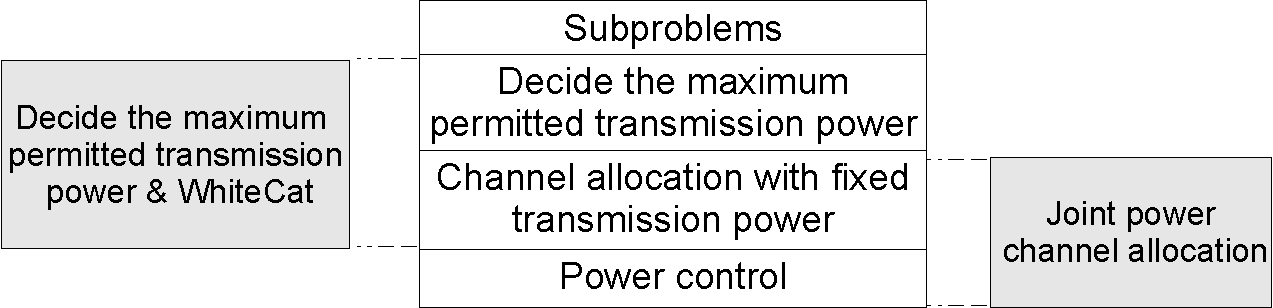
\includegraphics[width=\linewidth]{evaluation_content.pdf}
  \caption{The evaluation contents in this section, the left part is discussed in Section~\ref{MaxPower_whitecat} and the right part is in Section~\ref{joint}. 	}
\label{evaluationContent}
\end{figure}

The evaluation setting is as follows.
A square area which is 60km x 60km is divided into 16 square blocks evenly, for each block there is one WBS locating in the middle of it. 
Same mount of end terminals distributed in each minor block.
The terminals don't necessarily choose the WBS which is nearest to them to obtain service, in stead they choose the WBS to join, which provides the strongest \gls{RSSI} at them.
There is a 20km wide rim area around the square area, where the interference measurement devices for TV receiver are randomly located.
The number of such interference measurement devices is the same with the number of channels in the system, each device works on one channel.
The locations of WBSs and TV contours are illustrated in Fig.~\ref{sim:layout}.
WBSs' locations are fixed, but the locations of interference measurement devices for TV receivers, the end terminals, and the sequence for WBS to update are randomly decided in each run.
Simulations are conducted for 50 times.

\begin{figure}[h!]
  \centering
  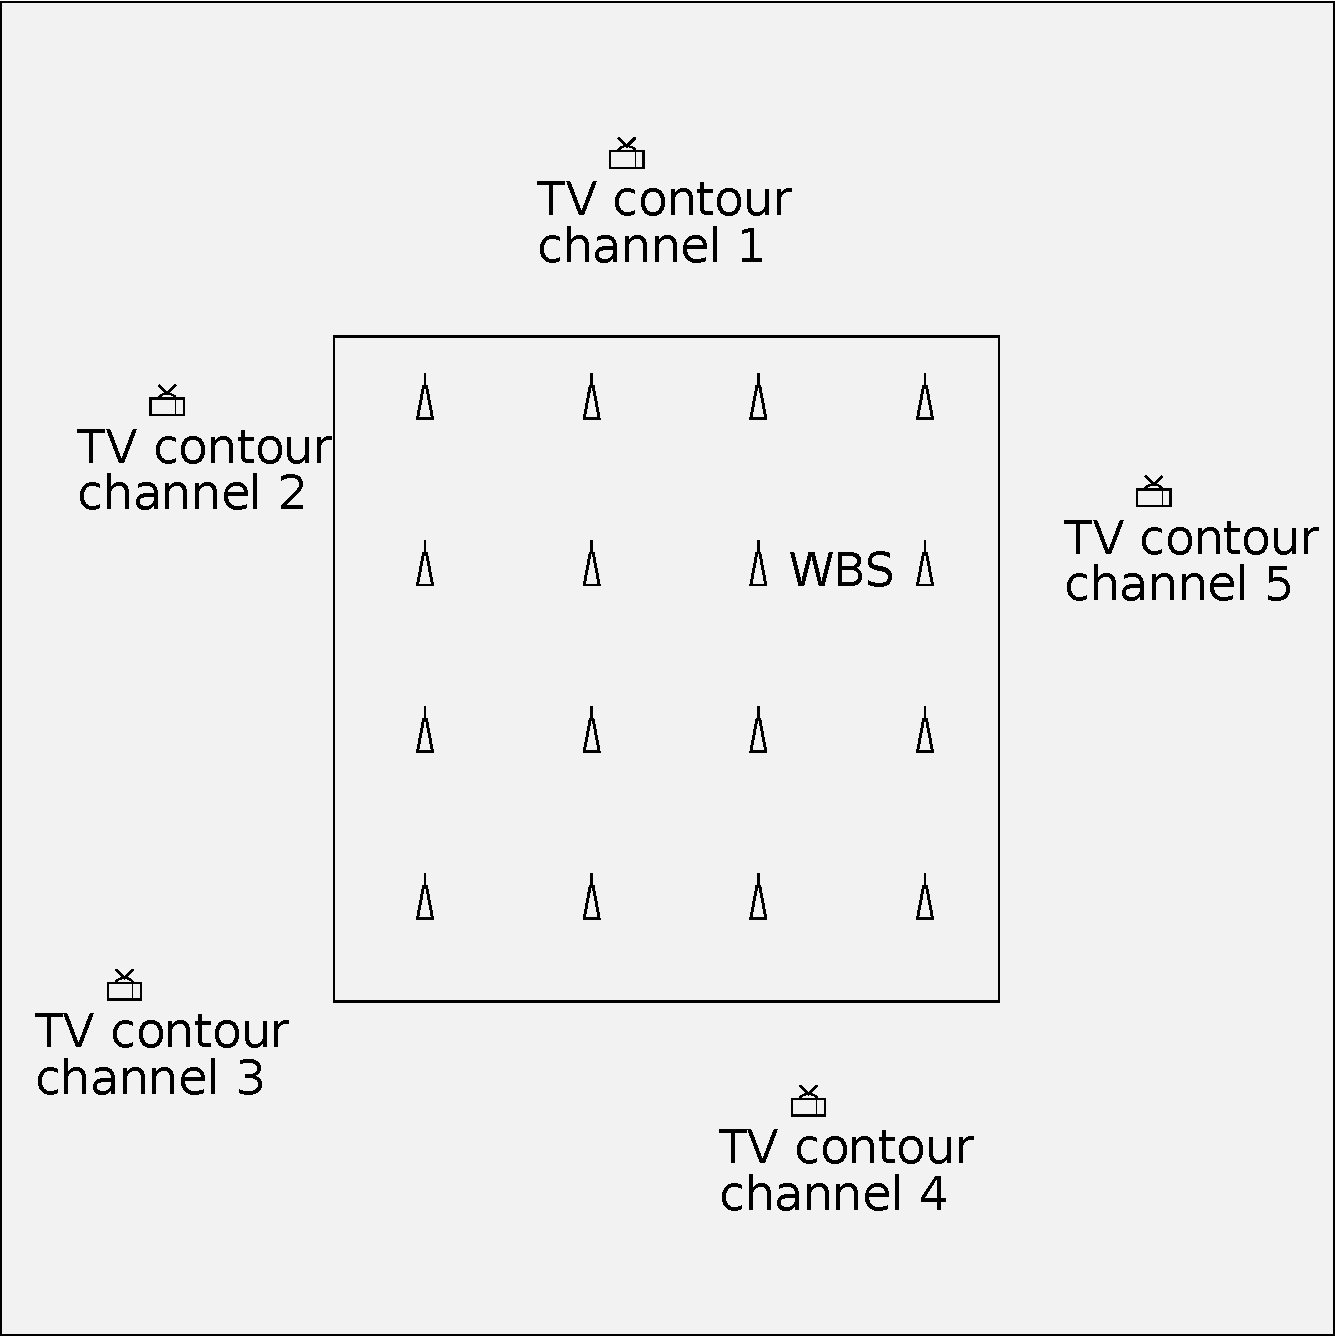
\includegraphics[width=0.5\linewidth]{layout.pdf}
  \caption{Layout of WBSs and TV contours}
  \label{sim:layout}
\end{figure}

The other parameters are listed in Table~\ref{6}.

\begin{table}[!h]
\centering
\begin{tabular}{|l|r|}
  \hline
  Number of channels 						& 5 \\
  Number of WBSs							& 16\\
  Noise 									& $10^{-12}$W \\ % -90dbm
  Length of side the square to locate WBSs		& 60km\\
  Distance between quasai terminal and WBS 	& 7km \\
  Interference threshold on TV contour 		& $10^{-7}$W \\ % -67dbm
  Path loss factor 							& 2 \\
  Standard deviation in flat shadowing		& 8\\
  Minimal WBS transmission power~\footnotemark{} 			& 4W \\
  Maximal WBS transmission power 			& 40W \\
  Number of end terminals in network 		& 800 \\
  \hline
\end{tabular}
\caption{Simulation parameters}
\label{simulationparameter}
\end{table}
\footnotetext{minimal and maximal power here denote the power level restricted by the specification of hardware.}

\subsection{Maximal Permitted Power Decision and the Distributed Channel Allocation Schemes}
\label{MaxPower_whitecat}
In this section, we will firstly evaluate the convex optimization and linear optimization proposed in Section~\ref{powermap} to see which is the better choice to decide the maximum permitted transmission power, the adopted metrics are average power consumption, and SINR on end users where channel allocation is executed.
Then with the decided better method, we compare given the power map, how do the channel allocation schemes perform.
%Respectively with the power map obtained from linear programming and convex programming, we execute channel allocation problems.
We compare our proposed channel allocation scheme \textit{whiteCat} with three other distributed schemes, the random allocation scheme, \textit{whiteCase} and No-regret learning, besides, centralized optimization is used to obtain global optima.

\begin{itemize}
\item \textit{WhiteCase}:  \underline{White}space \underline{c}hannel \underline{a}llocation \underline{se}lfish, where each WBS selfishly updates its channel to achieve the best (as to the considered problem, smallest) possible utility based on Formula~\ref{selfishutility}.

\item \textit{Noregret learning}: Each WBS maps the probability of choosing each strategy to a certain proportion of the regret which the WBS may have if it doesn't choose that strategy, and the WBS choose the strategy with the biggest probability.  
WBSs update such mapping dynamically and this approach converges to correlated equilibrium. 
Please refer the original paper \cite{hart00correlatedeq} for details.
		
\item \textit{Quadratic optimization}: centralized quadratic optimization introduced in Section~\ref{03_centralized_ca}.
\end{itemize}


\subsubsection*{The Choice of Radius of Auxiliary Circles, quasiSINR of WBS, and SINR on End Users}
The usage of quasiSINR exempts WBSs from taking care the SINR on the end terminals.
A WBS's quasiSINR is related with WBS's location and the radius of auxiliary circle.
Figure~\ref{radius} illustrates the effect of using different radii of the auxiliary circle on the data rate can be achieved by end terminals.

\begin{figure}[h]
\centering
\subfigure[quasiSINR of WBSs]{
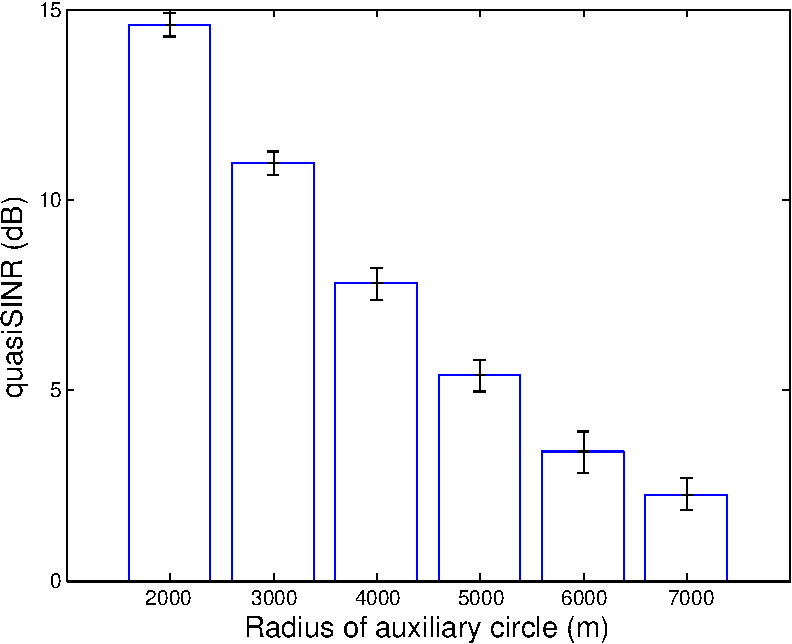
\includegraphics[width=0.435\linewidth]{qusaiSINR_with_radius.pdf}
\label{qusaiSINR_with_radius}
}
\subfigure[Data rate of end terminals when applying whiteCat]{
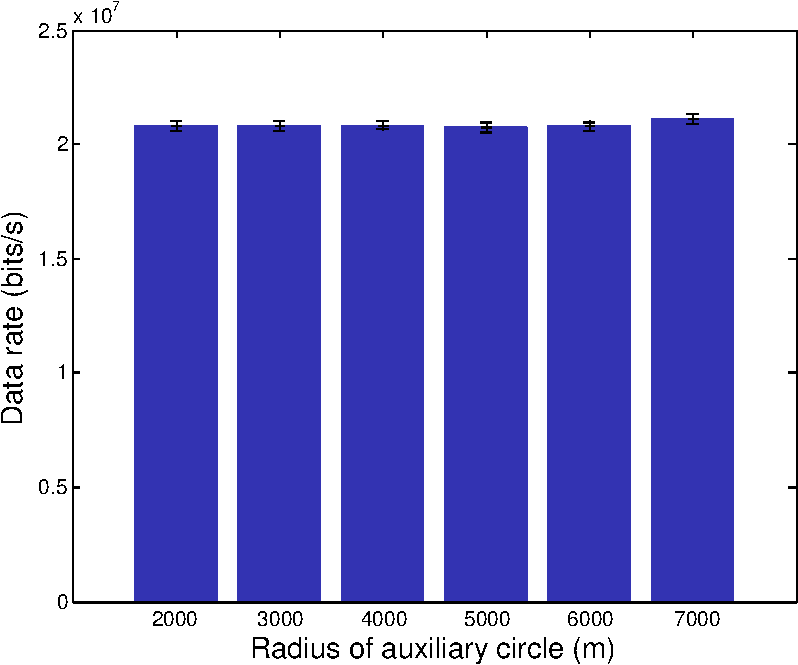
\includegraphics[width=0.435\linewidth]{sinr_on_endusers_with_radius.pdf}
\label{sinr_on_endusers_with_radius}
}
\caption[]{The effects of different radii of auxiliary circle on end terminals' data rate. Maximum permitted power is obtained by solving convex optimization. WhiteCat is used to assign the channels.}
\label{radius}
\end{figure}

Subfigure~\ref{qusaiSINR_with_radius} shows WBSs' quasiSINR decreases when the radii of auxiliary circles increase.
Subfigure~\ref{sinr_on_endusers_with_radius} illustrates the choice on radius of auxiliary circle don't influence the performance of whiteCat.
In the following simulation, we fixed the radius at 6000 m.

     


\subsubsection*{Performance of Channel Allocation Schemes}
In Section~\ref{powermap}, two different optimization formulations are introduced to obtain the maximum permitted transmission power for WBSs, \ie convex optimization and linear optimization respectively.
In Figure~\ref{lpcvx}, we have seen that the convex optimization generates power levels which distribute evenly between the minimum and maximum transmission power levels configured by the hardware, while, the majority of the power levels generated by linear optimization are either the minimum or maximum transmission power.
In this section we run the channel allocation schemes with the maximum permitted power levels obtained from convex and linear optimization respectively.
The simulation in this subsection carries twofold meanings.
The first is to see which maximum permitted power decision method outperforms the other, the second is to evaluate the performance of the channel allocation schemes.
The adopted metrics are the SINR on end terminals and transmission power consumption.


%we apply convex programming and linear programming to decide the maximal transmission power, and then the 4 distributed schemes are executed.

\subsubsection*{Comparison of the Methods for Maximum Permitted Transmission Power}
%We simulate the 4 distributed spectrum allocation schemes with the  map obtained from , and then tell which maximal power map generation outperforms based on the performances of the 4 spectrum allocation schemes.
 
Figure~\ref{transPower} depicts the power consumption of the channel allocation schemes which work with the two groups of maximum permitted transmission power decided by linear and convex problems respectively.
When given maximum permitted transmission power, whiteCat and the centralized optimization scheme consume the least energy.
The schemes utilize less transmission power with the maximum permitted transmission power decided by convex optimization.
%
Figure~\ref{qusaiSINR} shows the quasiSINR of WBSs.
The centralized optimization scheme achieves the highest quasiSINR, because the optimization formulation~\ref{QLP} obtains the global optima.
 \begin{figure}[h!]
    \centering
      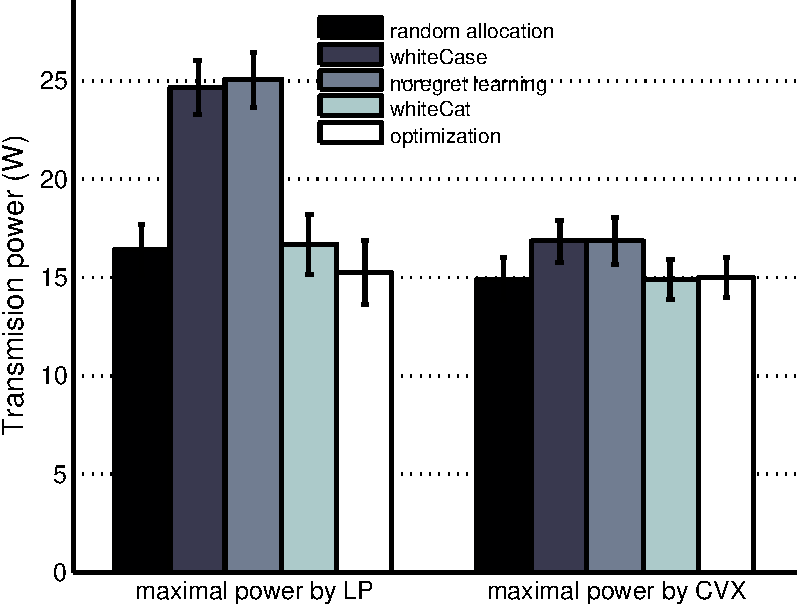
\includegraphics[width=0.7\linewidth]{transPower.pdf}
    \caption{Power consumed of WBSs by different distributed spectrum allocation schemes under different ways deciding the maximal transmission power map}
\label{transPower}    
  \end{figure}
  
   \begin{figure}[h!]
       \centering
       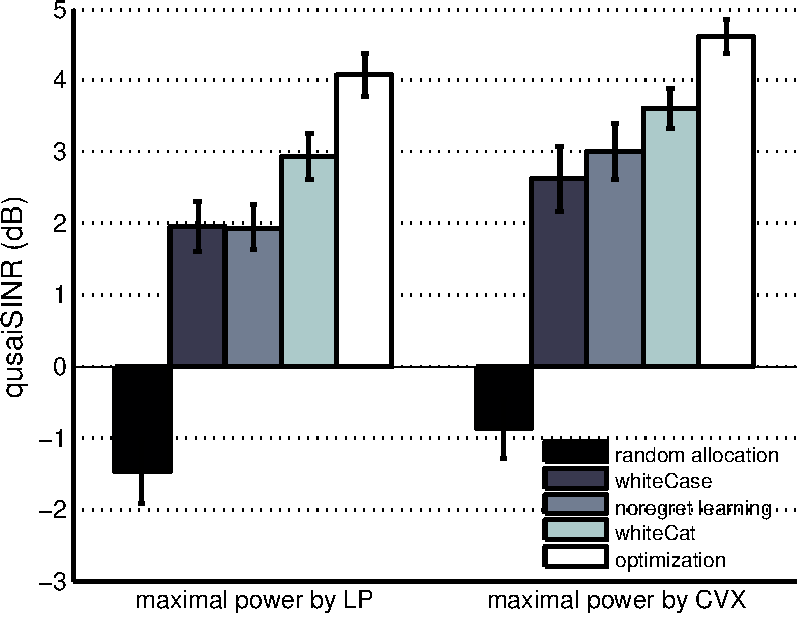
\includegraphics[width=0.7\linewidth]{qusaiSINR.pdf}
       \caption{QuasiSINR of WBSs achieved by different distributed spectrum allocation schemes under different ways deciding the maximal transmission power map}
	\label{qusaiSINR}
     \end{figure}
     
The average SINR on the end terminals is depicted in Figure~\ref{6000_sinr}.
When the given maximum permitted transmission power, whiteCat and the centralized optimization achieve similar and the best performance among the schemes.
It is also noticed that, the maximum permitted transmission power decided by linear optimization helps the channel allocation schemes achieve better SINR.
     \begin{figure}[h!]
       \centering
       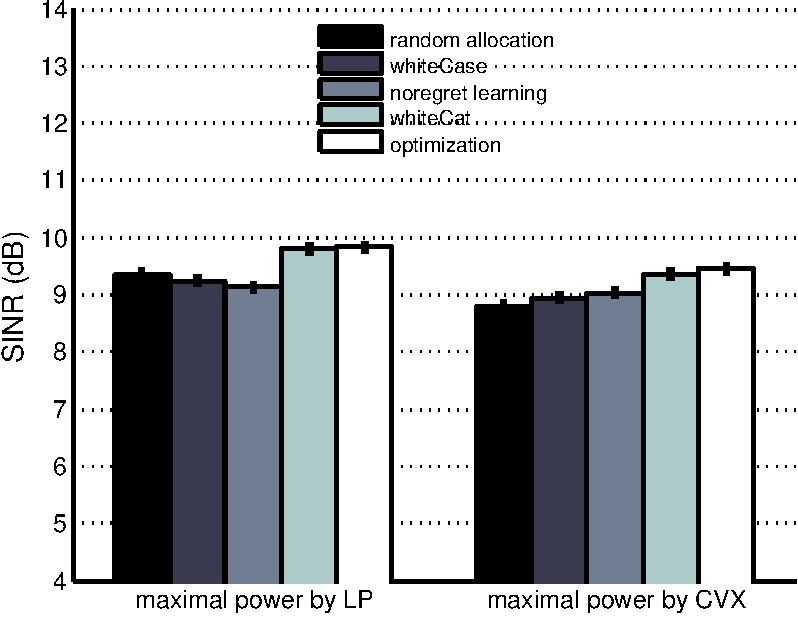
\includegraphics[width=0.7\linewidth]{6000_sinr.pdf}
       \caption{SINR on end terminals achieved by different distributed spectrum allocation schemes under different ways deciding the maximal transmission power map}
	\label{6000_sinr}
     \end{figure}

  \begin{figure}[h!]
     \centering
     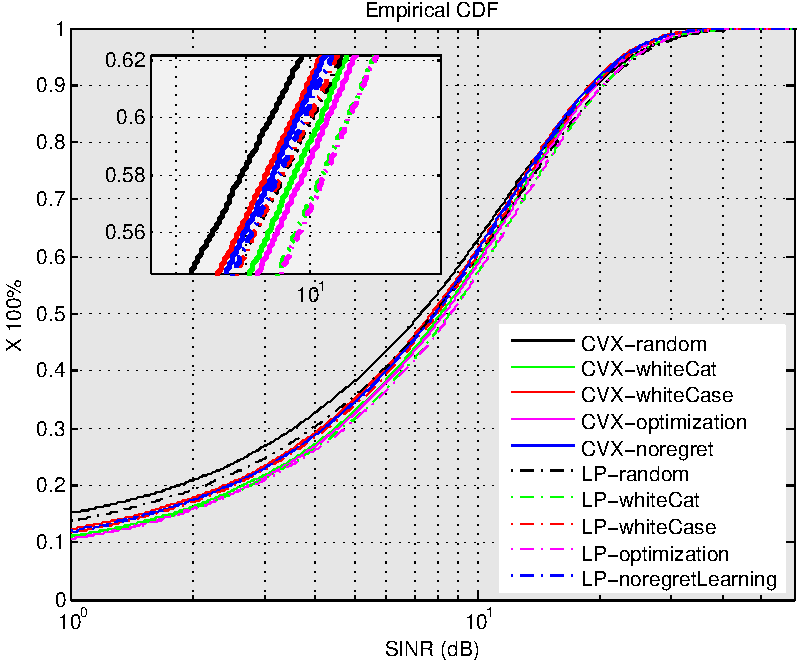
\includegraphics[width=0.7\linewidth]{6000_sinr_cdf.pdf}
     \caption{CDF of SINR on end users obtained by different CA schemes under different methods to decide the maximal transmission power map}
     \label{6000_sinr_cdf}
  \end{figure}

The empirical cumulative distribution function curve of SINR on end terminals is drawn in Figure \ref{6000_sinr_cdf}.
%where the X axis represents SINR level, and the Y axis shows the cumulative proportion of end terminals whose SINR equals or smaller than that level. 
The SINR achieved by WhiteCat and the centralized optimization is stably higher than that obtained from other schemes.
For example, the 20\% and 80\% percentile of the SINR achieved by WhiteCat and the centralized optimization are 0.5 to 1 dB higher than the other channel allocation schemes.
%The curves show that except for the random method, all three other distributed schemes perform better in low SINR area (SINR $<10 dB$) with convex formulation, while worse in the high SINR area. 
%Hence we adopt convex formulation to decide the maximum transmission power in the following simulation.



%\subsubsection*{Comparison of Channel Allocation Schemes }
%After deciding the maximum permitted transmission power on each channel for each WBS, the data center distributes this maximum power map to all WBSs, and trigger the procedure of distributed channel allocation. 
%
%
%
%The performance of the five spectrum allocation approaches working with the maximum transmission power map calculated from convex formulation is elucidated in the right part of both Fig.~\ref{sim:group1_power} and \ref{transPower}. 
%We can see that whiteCat consumes 12\% less transmission power than WhiteCase and No-regret learning schemes, whereas better QuasiSINR is obtained. 
%The cumulative distribution function curve of SINR on end terminals with convex programming is presented in Fig.~\ref{group1_sinr} with solid curves.
%It can be seen that for any cumulative proportion under 90\%, the corresponding SINR level caused by whitecat on end terminals is slightly (around 0.5-1 dB) but stably higher than that obtained by WhiteCase and No-regret schemes, and 3 dB higher than that in random scheme.
%
%In each run of simulation, average value of the 20 \% end terminals with the worst SINR is recorded, and the averaged such value over 100 simulations is illustrated in Figure \ref{group1_worst20sinr} which shows whiteCat achieves better performance for the worst suffered end terminals than WhiteCase and No-regret approaches.
%
%\begin{figure}[h]
%  \centering
%  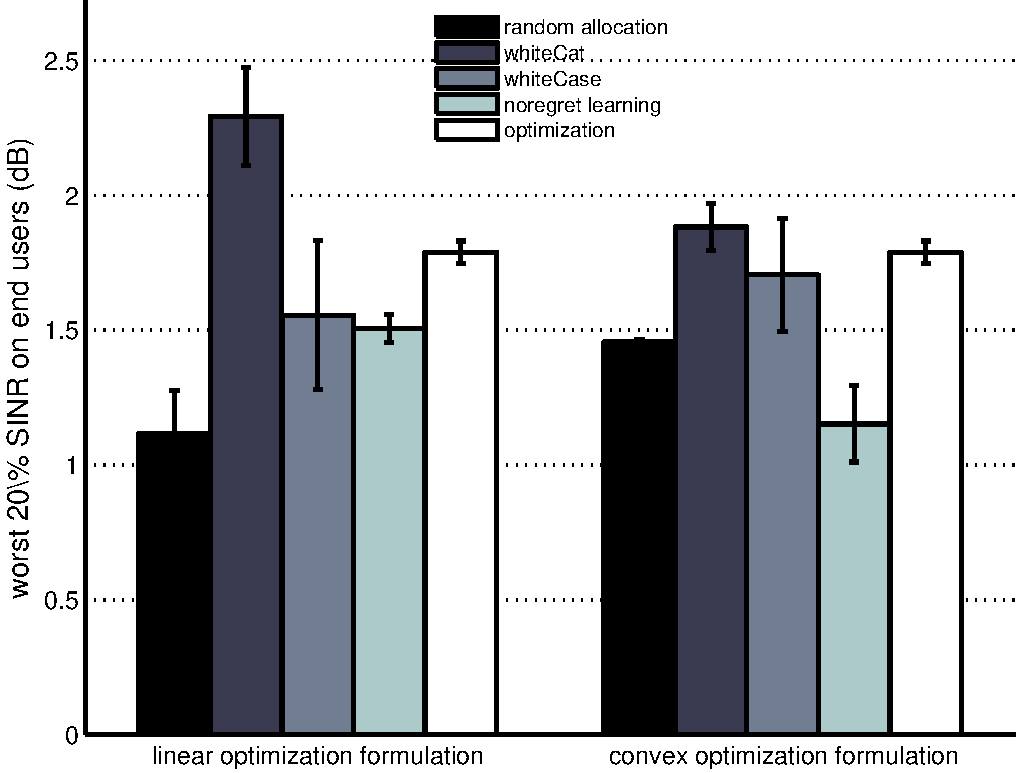
\includegraphics[width=0.8\linewidth]{1.pdf}
%  \caption{The average SINR of the 20\% worst end terminals}
%\label{group1_worst20sinr}
%\end{figure}
%
%

\subsubsection*{Convergence Speed}

%Complexity: 
%For each player, there are at most $(n-1)*|\mathcal{C}|$ resources available for usage, while, because the produced congestion on each resource is independent on channel, in other words, the congestions involving the same pair of players are quantitatively identical, there are only $(n-1)$ quantitatively different congestions on one player's resources. So, the number of combinations with quantitatively non-identical congestions involved with that player is $2^{(n-1)}$, accordingly there are totally $n*2^{(n-1)}$ quantitatively different congestions for the whole the problem. We adopt the method of \cite{LectureA}, which resorts the congestions in a increasing sequence, and replaces the original congestions with integer values starting form 1. We call the integers as \textit{new} congestions. In this way the preferences of the players are preserved and we can find easily the biggest possible congestion is $n*2^{(n-1)}$, which is the upper bound for the number of steps towards convergence.
In the congestion game where scheme whiteCat is derived, each player (WBS) has at most $(n-1)*|\mathcal{C}|$ resources available for usage, thus there is no polynomial steps converging to NE, while, simulation shows the algorithm can quickly converge to NE when the number of WBS is up to 100. 
%Figure \ref{100converge} shows that for 100 WBSs, whitecat executes at most 5 iterations (in one iteration all WBSs update their choices). 
%Figure \ref{convergeComp} depicts one instance of simulation, where whiteCat converges quickly, No-regret produces oscillation but converges finally, while WhiteCase can not converge thus has to be enforced stop after 16000 updates. %\todo{replot}%, whereas 
%
Table~\ref{convergencespeed} shows the average number of steps needed before convergence in 100 runs of simulations.
As to whiteCat, we account each WBS accessing the base station (refer to \ref{whitecat}) as \textit{one step}.
We compare the convergence speed of WhteCat with no-regret learning, the scheme derived from potential game~\cite{pimrc_2012} and whiteCase.
Note that the potential game scheme is to solve joint power and channel allocation problem, as it is developed with game theory, it is reasonable to see its convergence speed.
As there is no guarantee for WhiteCase to converge, we stop the channel allocation process after 16000 steps (1000 rounds).

Table~\ref{convergencespeed} tells that whiteCat is two times faster than the scheme derived from potential game, and 20 times faster than no-regret learning scheme.
The relatively smaller confidence interval shows that whiteCat's convergence is not affected by different network configurations.
Fast converge is attributed to the working style of WBSs whcih access the database to get the information of other WBSs, thus the distributable decision involves a part of the global information of the network.
Thus, we can see that the speed up of convergence is due to the overhead caused by accessing the database.


Figure \ref{convergeComp} depicts one instance of the convergence processes of three schemes.
The Y axis is the summed utility of all WBSs.
We can see whiteCat decreases the summed utility constantly, and the channel allocation process ceases after 38 times of updates.
Whereas, noregret learning scheme takes 120 steps before convergence, and whiteCase fails to converge.
%XXXXXX ***************
%Notice that there is a slight rise when the value on the X-axis is 35, which comes from the difference between \ref{compare} and \ref{allPotential}.
%XXXXXX ***************
\begin{table}[!h]
\centering
\begin{tabular}{|l|c|c|c|}
  \hline
  Scheme			 						& Average steps 	 		& 95\% CI			&Average time (s)\\
    \hhline{|=|=|=|=|}
  whiteCat									& 58						& 5.6						&2\\\hline
  noregret									& 1916						& 1541						&144\\\hline
  PotentialGame~\cite{pimrc_2012}			& 120						& 10						&4\\\hline
  optimization-LINDO						& -                         & -                         &40\\\hline
  whiteCase 								& 4587 						& 2742						&50\\  
  \hline
\end{tabular}
\caption{Convergence speed of the distributed channel allocation schemes. As to the distributed scheme, the time involved to communicate with database is note considered and included.}
\label{convergencespeed}
\end{table}

%\begin{figure}[h!]
%\label{100converge}
%  \centering
%  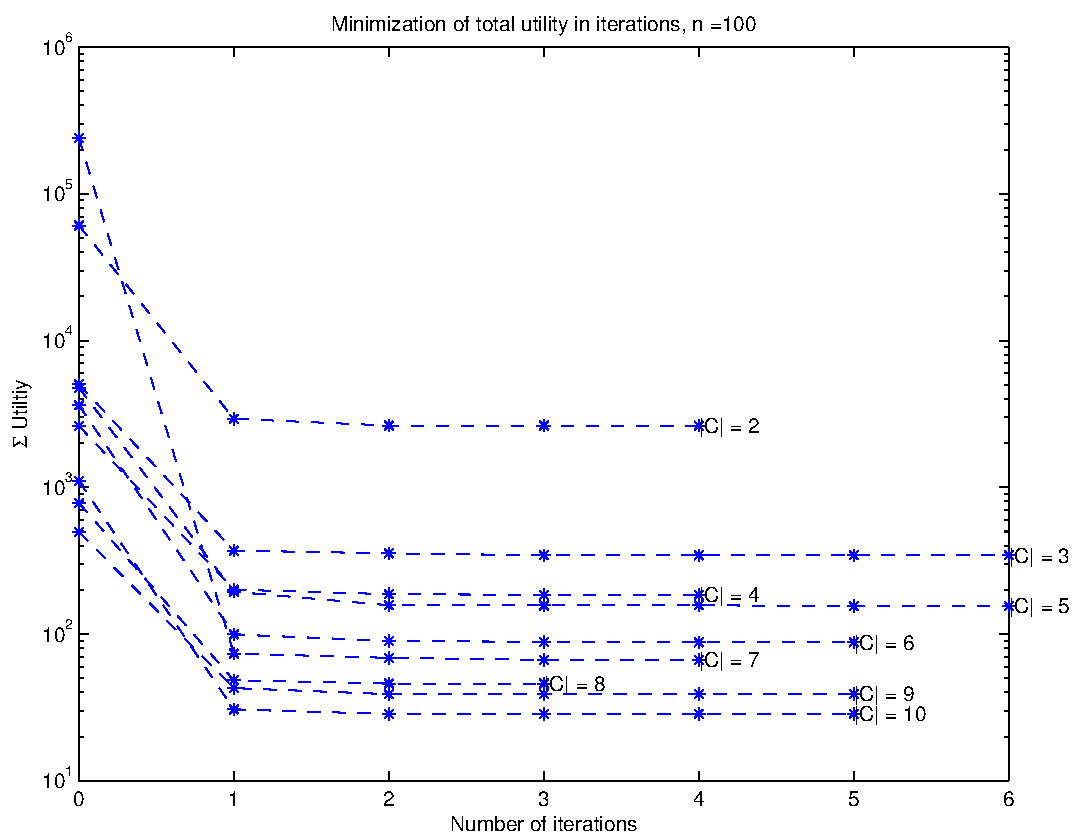
\includegraphics[width=0.65\linewidth]{CAConverenge100.pdf}
%  \caption{100 WBSs, 2-10 channels}
%\end{figure}

\begin{figure}[h!]
  \centering
  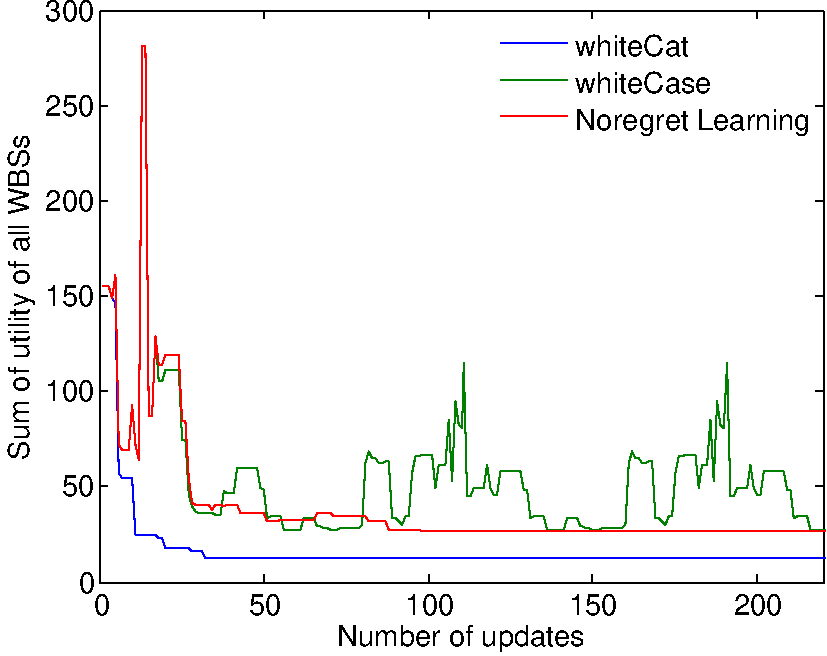
\includegraphics[width=0.8\linewidth]{convergence.pdf}
  \caption{Convergence process of three different schemes in one simulation.}
\label{convergeComp}
\end{figure}




\subsubsection*{Stability of SINR in Convergence Process}
WBS provides service to end users in the process of channel allocation. 
A certain SINR corresponds to certain transmission configurations like modulation type and data rate. 
The oscillation of SINR resulted from WBS changing the working channel during the convergence process may cause reconfiguration, reduced throughput or delay variance, which is not preferred.
We propose a metric \textit{Cost of Oscillation} (\gls{COS}) to represent the stability of SINR in the converging process.
Assuming each update of channel takes 1 time unit, the variance of SINR of end user $i$ at time $t+1$ is \[\varDelta  \gamma_i(t+1)=\mid\frac{\gamma_i(t+1)-\gamma_i(t)}{\gamma_i(t)} \mid\]. 

The COS value for one network applied with a certain channel allocation scheme is,
\begin{equation}
\label{cos}
			COS = \sum\limits_{t=1}^T   \sum\limits_{i\in \mathcal{N}} \varDelta  \gamma_i(t)
			\end{equation}
$\gamma_i(0)$ is the SINR for $i$ before starting channel allocation.
The variance of SINR in channel allocation process is shown in table \ref{costable} from which we can see WhiteCat achieves only 6\% of oscillation on SINR compared with No-regret approach.
\begin{table}[!h]
\centering
\begin{tabular}{|l|c|c|}
  \hline
  Scheme			 						& COS 					& 95\% confidence interval\\
    \hhline{|=|=|=|}
  WhiteCat									& 8850					& 2984\\\hline
  No-regret									& 145460				& 1541\\\hline
  WhiteCase 								& 246790 				& 168050\\ 
  \hline
\end{tabular}
\caption{Variance of SINR during the convergence process}
\label{costable}
\end{table}



\subsection{Performance of Joint Power and Channel Allocation}
\label{joint}
%: Cascaded Distributed Schemes vs. Joint Distributed/centralized schemes

As introduced in section~\ref{powerAllocation}, after channel allocation is conducted, transmission power is adjusted in a distributive manner.
In other words, power and channel allocation is executed with two cascaded distributed schemes.
%Distributed channel allocation schemes, along with the power adjustment, are compared with two other schems.
As comparisons, we implement two joint power channel allocation schemes.
One is centralized optimization introduced in section~\ref{opt_channelAndPower}, which is used as upper bound in the comparison.
The other comparison is distributed joint power and channel allocation scheme~\cite{pimrc_2012} which is introduced in Section~\ref{decomposition_relatedwork}, we name it as \textit{potentialGame}.
We need to point it out that, scheme \textit{potentialGame} doesn't aim to improve the SINR on end terminals, but on the sum of produced and received interferences.
The performance of joint channel and power allocation schemes are presented in Fig.~\ref{CAPA_utility}, \ref{CAPA_power} and \ref{joint_SINRcdf} in terms of total utility, power consumption and achieved SINR on end users respectively.

Figure~\ref{CAPA_utility} illustrates the comparison of the cascaded solutions, \ie channel allocation and the following power control, in terms of the total utility in the network.
We can see that our proposed scheme \textit{whiteCat+dpa}, the cascaded channel and power allocation method falls behind the cascaded channel allocation optimization and power allocation, and the joint channel and power allocation optimization, but outperforms all the other distributed solutions.
Note that the \textit{potentialGame} method along with power control results the worst performance, the reason is the objective adopted by \textit{potentialGame} is to minimize the sum of received interference in the network, thus the performance on summed utility demonstrates randomness.
Figure~\ref{joint_SINRcdf} draws the CDF of SINR on end users when applying different channel allocation and power allocation schemes.
it is clear that our proposed approach achieves the best among the distributed schemes, and only worse wore than the schemes which involves centralized optimization.



\begin{figure}[h!]
  \centering
  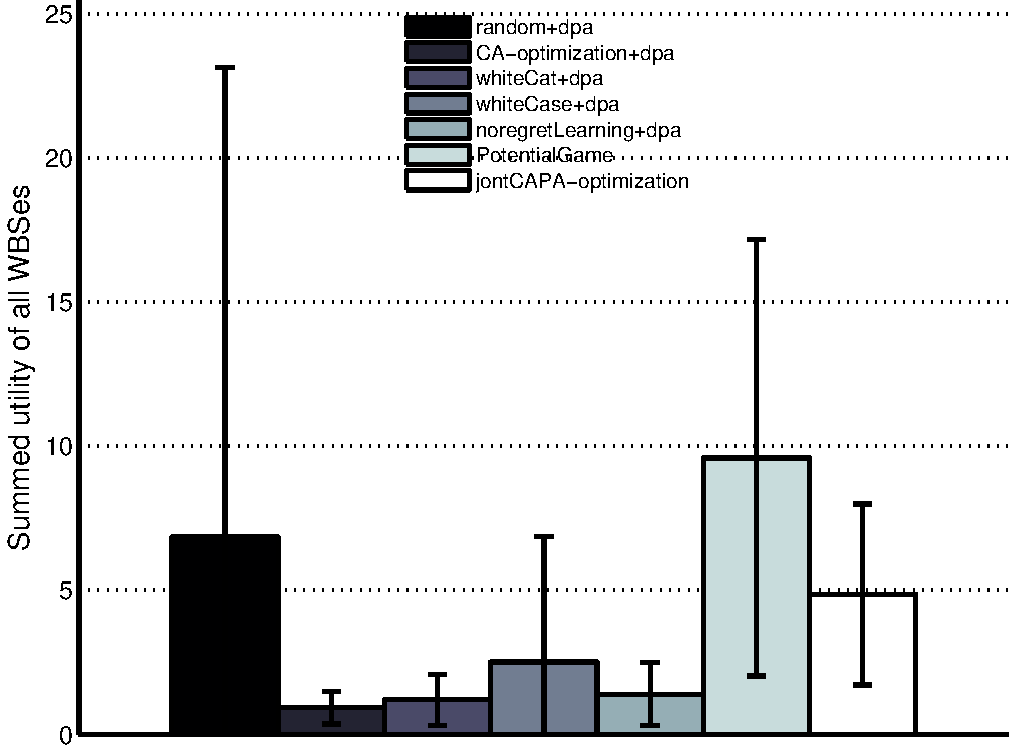
\includegraphics[width=0.8\linewidth]{16.pdf}
  \caption{Summed utility of all WBSs, which is the objective in problem~\ref{problem}. dpa in legend represents distributed power allocation}
\label{CAPA_utility}
\end{figure}



%\begin{figure}[h!]
%  \centering
%	\subfigure[After channel allocation]{	  \label{summedU:sub1}	  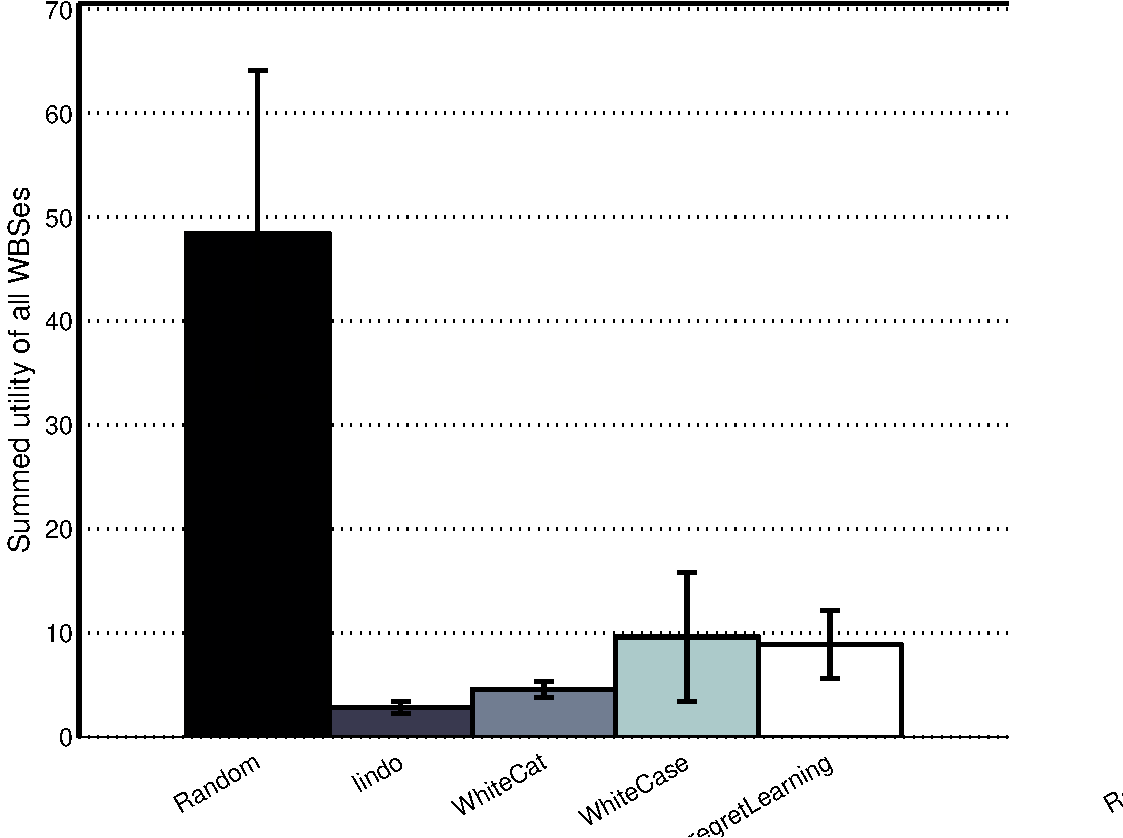
\includegraphics[width=0.47\linewidth]{12.pdf}}
%	\subfigure[After channel and power allocation]{  \label{summedU:sub2}	  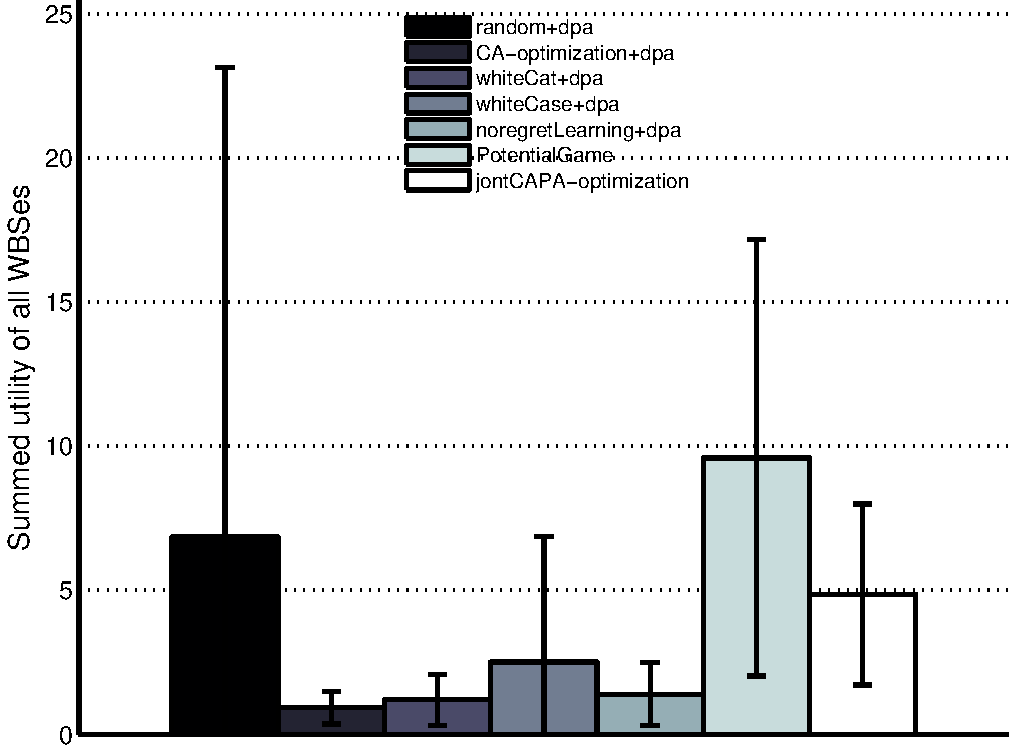
\includegraphics[width=0.47\linewidth]{16.pdf}}
%  \caption{summed utility of all WBSs, which is the objective in problem~\ref{opt}f{opt}}
%  \label{utility}
%\end{figure}



\begin{figure}[h!]
  \centering
  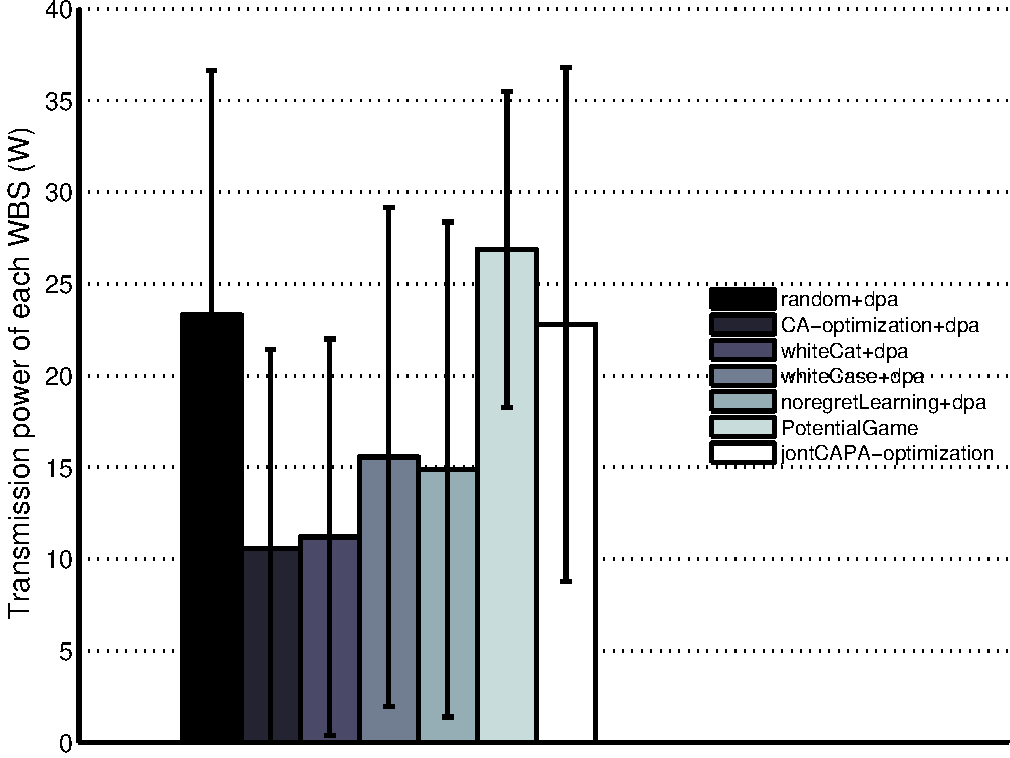
\includegraphics[width=0.8\linewidth]{14.pdf}
  \caption{Average transmission power of one WBS}
\label{CAPA_power}
\end{figure}
%
%%\begin{figure}[h!]
%%  \centering
%%  	\subfigure[After channel allocation]{\label{power:sub1}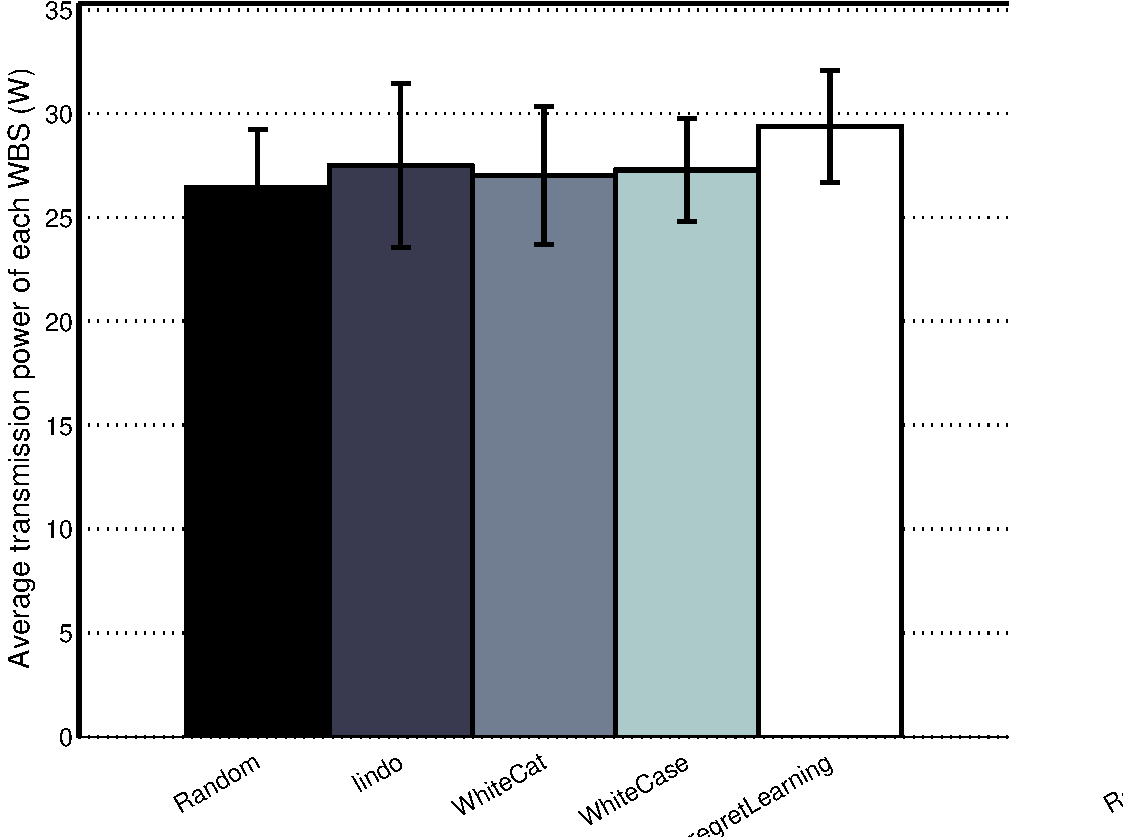
\includegraphics[width=0.47\linewidth]{10.pdf}}
%%  	\subfigure[After channel and power allocation]{\label{power:sub2}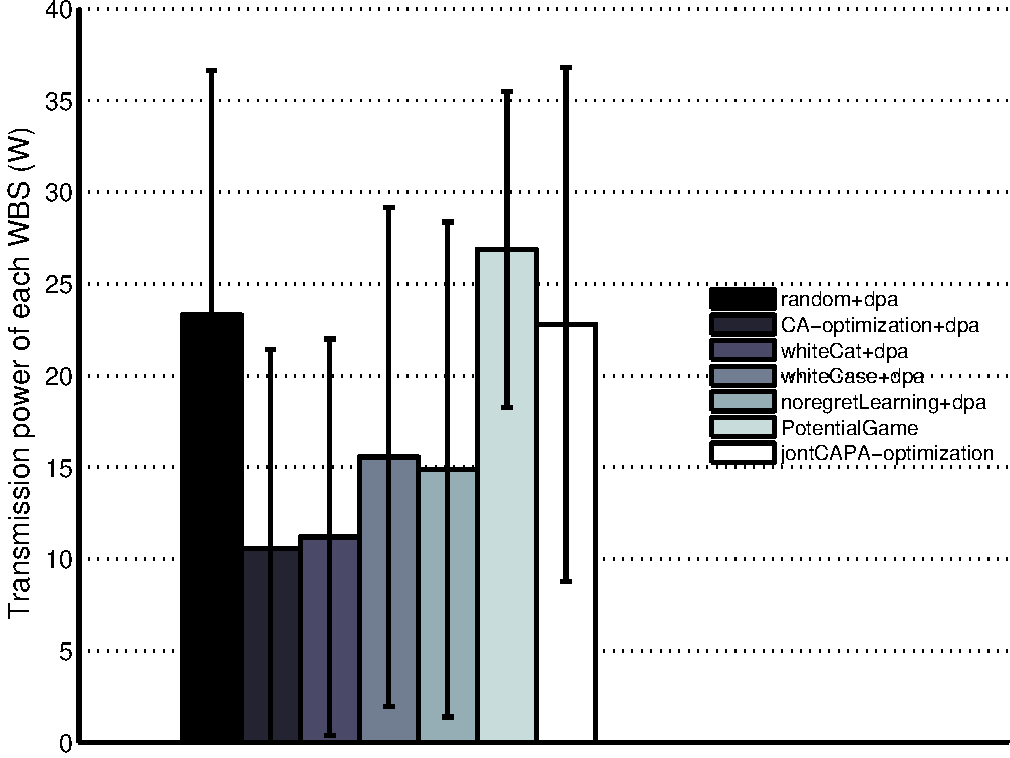
\includegraphics[width=0.47\linewidth]{14.pdf}}  	
%%  \caption{Average transmission power of one WBSs}
%%  \label{power}
%%\end{figure}
%
%\begin{figure}[h!]
%  \centering
%  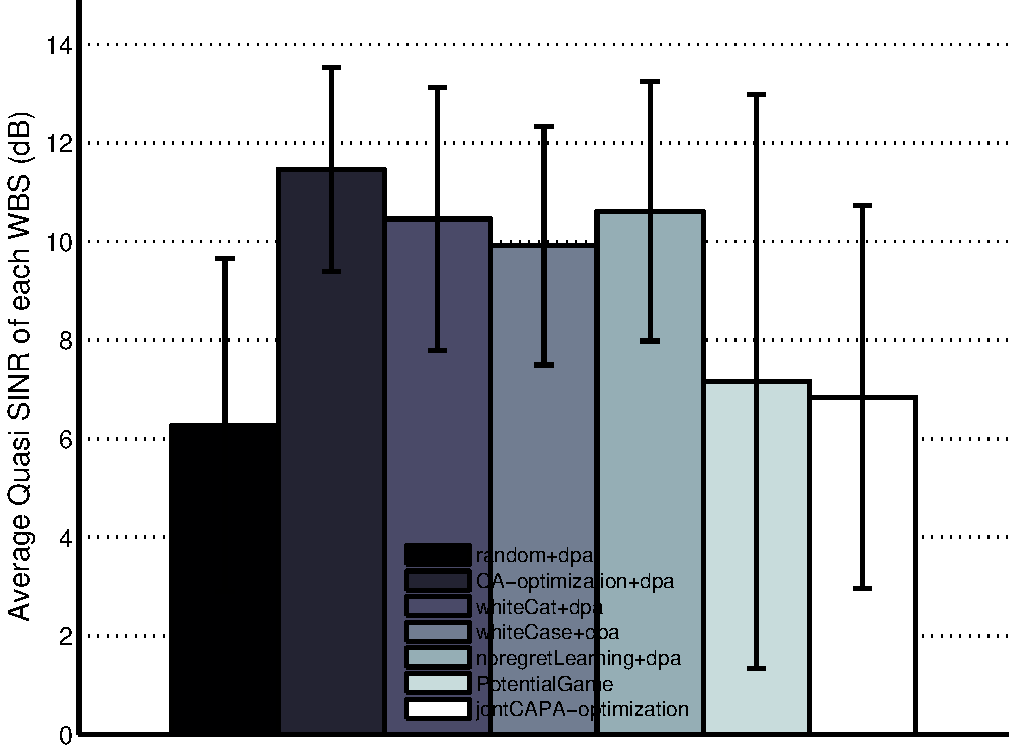
\includegraphics[width=0.8\linewidth]{15.pdf}
%  \caption{Average quasiSINR of a WBS}
%\label{CAPA_quasiSINR}
%\end{figure}


%Compare the two figures in Figure \ref{utility}, \ref{power},\ref{quasiSINR}, we can see that transmission power is reduced by 50\% to 70\% for all schemes except for the random selection scheme, and the utility and quasiSINR are almost the same.




%\subsection{Comparison between distributed and centralized scheme  }

%After comparing the performances of WhiteCat with the other two heuristic solutions, we have a look at the difference between these distributed approaches with the centralized optimization method. For these heuristic schemes, the sequence to update influences the final performance, while, it is very difficult to find out the optimal sequence which achieve the best performance, for our simulation configuration, the number of different sequence for 16 WBSs is $16!$ which has order of magnitude of 14. For demonstration purpose, we choose 100 different update sequences randomly for 100 times of simulation. In each simulation the sequence of WBS to update their channels is randomly decided be identical for all the 4 schemes. As solution of optimization has nothing to do with sequence, we only solve the optimization problem for once. We fixed the location of WBSs and PU contours, only leave the end terminals randomly scattered in the inner square area in each simulation. 

%Figure \ref{perf1} reflects the performance of power consumption, QuasiSINR, and standard deviation of QuasiSINR when we apply the different schemes to the network. The upper left subplot illustrates that Whitecat consumes the least power compared with the other heuristic schemes along with the centralized optimization scheme. Upper right subplot shows that whitecat can achieve better QuasiSINR than Whitecase and non-regret approaches, but about 10 \% worse than the solution obtained from LINDO. Unsurprisingly, randomly choosing channels leads to the worst performance on QuasiSINR. The subplot below depicts the standard deviation of QuasiSINR from the five schemes, we can see the standard deviation of QuasiSINR achieved by whitecat is bigger than whitecase, non-regret and centralized optimization, which can be explained by Figure \ref{cdf}. 

%Fig.~\ref{powerQuasiSINR} shows the average power consumption and average QuasiSINR over all WBSs and rounds of simulations. 
%WhiteCat consumes the least of power except for the random scheme. while, Lindo outperform others 
%\begin{figure}[h!]
%  \centering
%  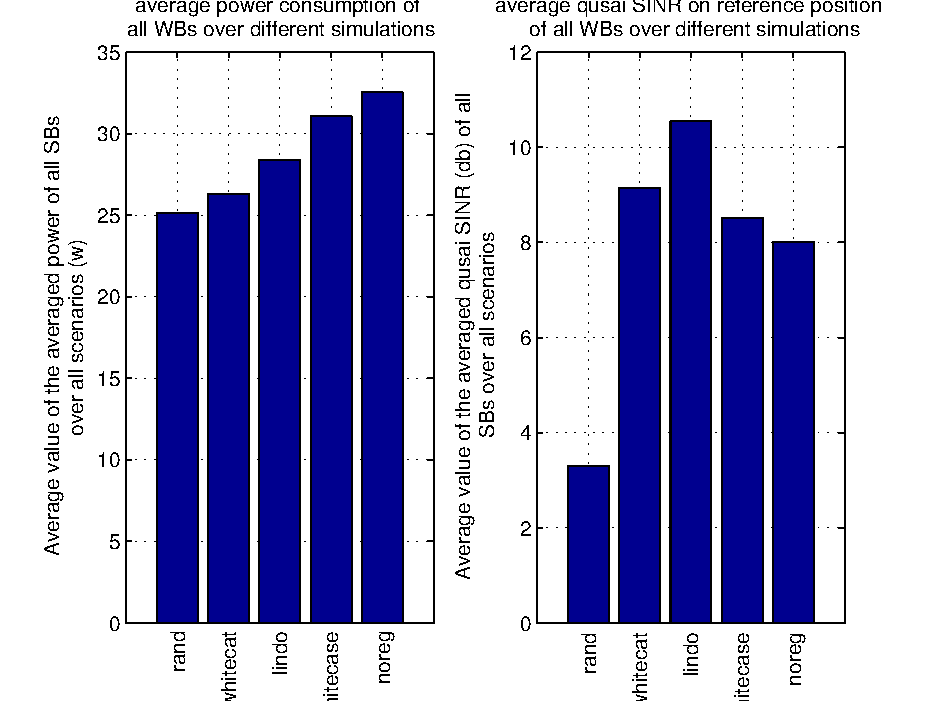
\includegraphics[width=1\linewidth]{powerQuasiSINR.pdf}
%  \caption{Average Power consumption and QuasiSINR}
%\label{powerQuasiSINR}
%\end{figure}

%Fig.~\ref{joint_SINRcdf} demonstrates the cumulative distribution of SINR on all end terminals, where the centralized optimization achieves 3 dB better SINR on end terminals than distributed schemes, which means there is still big space to improve the performance of decentralized approaches.

%\begin{figure}[h!]
%  \centering
%  	\subfigure[After channel allocation]{\label{fig:sub1}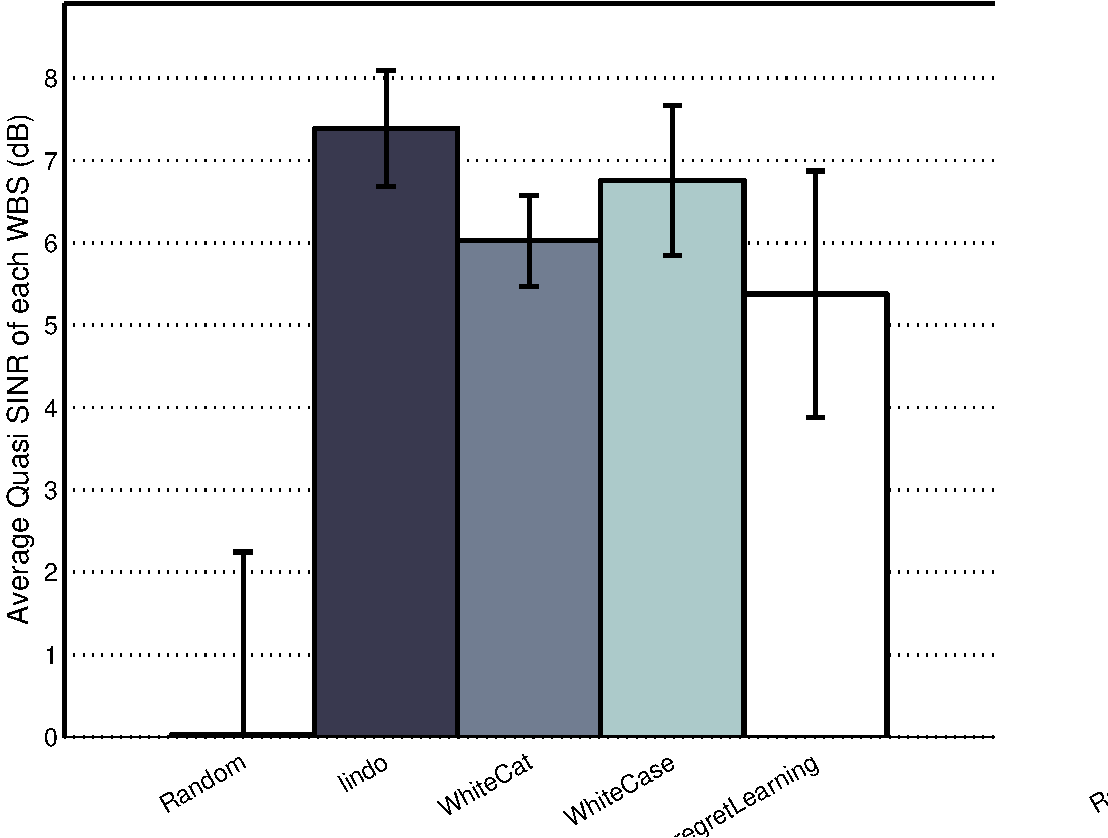
\includegraphics[width=0.47\linewidth]{11.pdf}}
%  	\subfigure[After channel and power allocation]{\label{fig:sub2}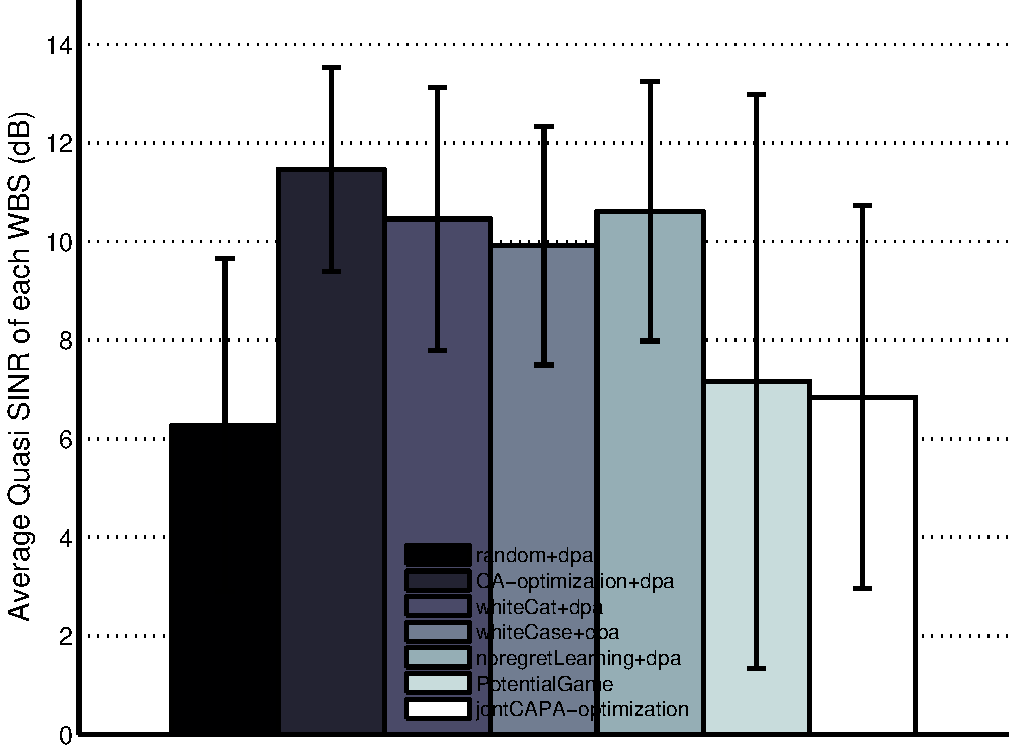
\includegraphics[width=0.47\linewidth]{15.pdf}}  	
%	  \caption{quasiSINR: SINR at the reference point}
%	  \label{quasiSINR}
%\end{figure}

%\begin{figure}[h!]
%  \centering
%      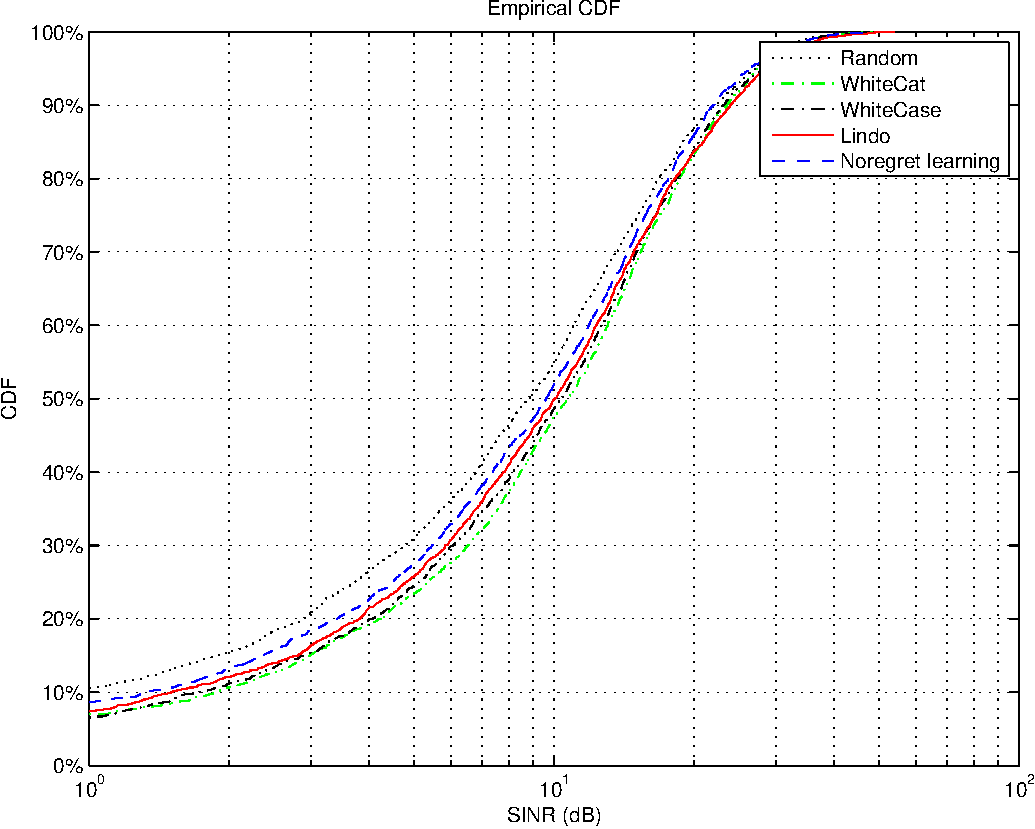
\includegraphics[width=0.9\textwidth]{20.pdf}
%  \caption{SINR on end users after channel allocation}
%\end{figure}

\begin{figure}[h!]
  \centering
      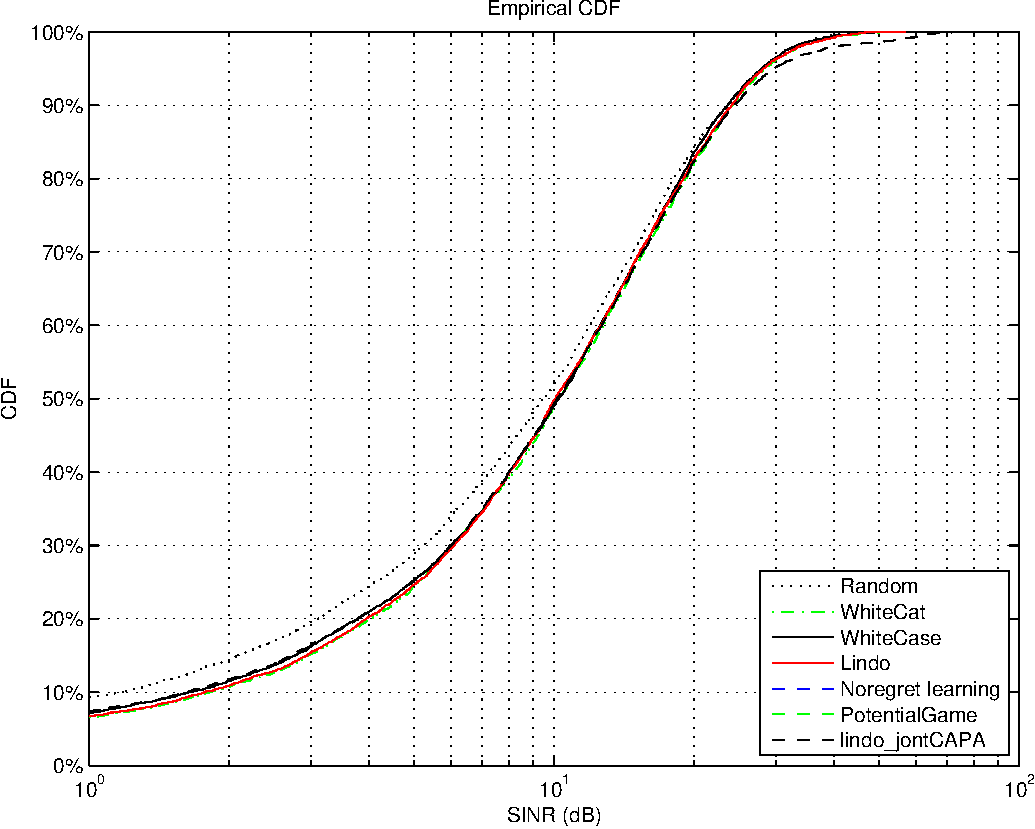
\includegraphics[width=0.9\textwidth]{24.pdf}
  \caption{Cumulative distribution of SINR on end users after channel and power allocation}
          \label{joint_SINRcdf}
\end{figure}

\section{Conclusions}
Congestion game is applied to analyse the channel allocation problem, where transmission power is not necessarily identical.
The proposed algorithm which is derived from the best response of the congestion game converges quickly, and achieves better performance than other distributed schemes.
Without consider the communication latency between WBSs and the database, this distributed scheme executes much faster than the centralized scheme.

In particular, we investigate the channel allocation problem in the context of utilization of TV white space.
Except for channel allocation, we also propose solutions for transmission power control for the cellular network which complies with IEEE 802.22 standard.
%With the centralized database, a centralized method to obtain the maximum permitted transmission power which complies with IEEE 802.22 standard is proposed.
%Then a distributed channel allocation algorithm is designed based on congestion game, where WBS can distributively choose the working channel which is associated with maximum permitted transmission power.
%The distributed channel allocation scheme outperforms several other distributed solutions, and obtains worse performance only than the centralized solution, while.

%A transmission power control procedure is conducted on the previous channel allocation.
%We investigate the performance of applying the combination of channel allocation and the power control.
%Our proposed channel allocation scheme together with power control achieve better performance than the other channel allocation scheme with the same power control scheme.
%The centralized joint channel and power scheme performs the best, but the problem is very difficult to solve.

%This solution makes full use of the infrastructure, the centralized database, and distributes the computation and decision making afterwards on channel and transmission power.





\chapter{ROBUST CLUSTERING of AD HOC COGNITIVE RADIO NETWORK}
\section{Introduction}
\label{intro}
%\todo[inline]{The first paragraph will be moved/integrated to INTRODUCTION chapter later.}
Cognitive radio (CR) is a promising technology to solve the spectrum scarcity problem~\cite{Mitola}. 
In CR systems, primary users access their allocated spectrum band whenever there is information to be transmitted. 
In contrast, CR users (forming cognitive radio networks, abbreviated as CRN) can only access primary channels after validating the channel is idle. 
This refers to the process of sensing a particular channel and verifying (with a previously specified probability of error) that it is not used by a primary user currently. 
This form of spectrum sharing is also referred to as opportunistic spectrum access.

%[Benefits of clustering]





%[clustering in crn] 
As introduced in Chapter~\ref{INTRODUCTION}, efficient spectrum sensing is identified as to be critical to the success of cognitive radio networks~\cite{Sahai_FundamentalDesignTradeoffs2006}.
Cooperative spectrum sensing is able to effectively cope with noise uncertainty and channel
fading, thus improves the sensing accuracy remarkably~\cite{Akyildiz_2011_CooperativeSpectrumSensing}.
Clustering is regarded as an effective method used in cooperative spectrum sensing~\cite{Sun07_clustering_spectrum_secsing, Zhao07}.
Collaborative sensing relays on the consensus of CR users within certain area, and decreases considerably the false sensing reports caused by fading and shadowing of reporting channel.
%As a result, more accurate sensing result can be obtained by collaborative sensing, and the improvement on spectrum sensing decreases the interference originating from CR users to primary users, which is highly desirable.
%Also,  prevents CR users from using channels that are occupied by primary users. 

Clustering is also efficient to let all CR users\footnote{User and node are used interchangeably in this chapter} within the same cluster stop payload transmission on the operating channel and initiate the sensing process, so that the all the CR nodes within the one cluster are able to vacate the channel swiftly when primary users are detected by at least one CR node residing in the cluster~\cite{willkomm08}.
With cluster structure, the possibility that one CR node interferes neighbouring clusters after vacating the channel due to primary node appearance is reduced~\cite{centralizedSharing80222}, as it can be notified by cluster head or other cluster members about the possible collision. 
Clustering algorithm has also proposed to support routing in cognitive ad-hoc networks~\cite{Abbasi_survey_07}.

%%[crn for clustering] 
%%due to attenuation of signal propagation, primary users can only be detected by CR users when they locate closely to CR users.
%In cognitive radio networks, secondary users which locate closely with each other are possibly affected by the same group of primary users, so that the availability of licensed spectrum is similar to them, \ie certain channels are available on each of them.
%The similarity of available spectrum on a group of neighbouring CR nodes, along with the benefit of collaborative decision among multiple nodes, leads to clustering as an effective approach for many applications.

%[robustness issue for clustering]
Except for the advantages brought in by clustering, there is an issue on clustering structure itself in cognitive radio network.
As the activity of primary users is controlled by licensed operators which are generally not known to CR users, the connectivity between CR nodes in a CRN is not guaranteed. 
For a pair of communicating CR nodes, whenever a primary user is detected to be operating on the working channel, CR nodes have to retreat that working channel.
The affected CR nodes switch to one other idle channel if there are available idle channels, if not, the communication is cut down.
As a result, when coexisting with primary users, the ability for one pair of CR nodes to maintain communication with licensed channels is totally decided by primary users' activity.

Although the communication among secondary users is vulnerable under the affection of primary users, which is objective in the eyes of secondary users, there is something can be done by secondary users when they form clusters. 
%Thus robustness of connection with licensed channels demonstrates to be objective from the perspective of secondary users.
To maintain one cluster operating on licensed channels, at least one common channel is available for all members in that cluster.
When the increase of channel occupation by primary users is assumed to be random, a cluster with more channels will stand ground with higher probability.
Thus the number of available common channels in the cluster indicates robustness of it when facing uncontrolled influence from primary users.
It is not difficult to see that forming clusters with different neighbours leads to different amount of common channels in the clusters.
As a result, how to form the clusters plays an important role on the robustness of clusters in CRN.

%Furthermore, the clustering algorithm also determines the connectivity between several clusters which ultimately determines the robustness of the entire network on the respect of connectivity. 

To solely pursue connectivity robustness against the primary users' activity, \ie to achieve more common channels within clusters, which is adopted by [xxxxxSOCxxxxxx], the ultimately best clustering strategy is ironically that each node constitutes one single node clusters.
%In that case, the common channels within cluster are the available channels available at that node's place.
Apparently this contradicts our motivation of proposing cluster in cognitive radio network.
This contradiction indicates that, the robustness discussed in terms of number of common channels carries little meaning when the sizes of formed clusters are not given consideration.
Besides, cluster size plays import roles in certain aspects.
For instance, cluster size is one decisive factor in power preservation~\cite{clustering_globecom11, EnergyEfficientClusteringRouting_2015}, and it is also influence the accuracy of cooperative spectrum sensing [xxxxxx].
Hence, cluster size should be given consideration when discussing cluster robustness against primary users.

In this chapter, a decentralized clustering approach ROSS is proposed.
ROSS is able to form clusters whose sizes are not far away from the desired size, and the generated clusters are more robust than other robust clustering scheme, \ie more secondary users residing in clusters against increasing affection from primary users.
Compared to previous work, ROSS involves much less control messages, and the generated clusters are significantly more robust.
In ROSS, cluster head is selected through coordination within its neighborhood, and then cluster membership is decided locally and its convergence is proved under game theoretic framework. 
%building more homogeneous clusters with respect to their size and forcing nodes with a high connectivity degree to the border of a cluster (making the cluster therefore more robust regarding connectivity loss to its neighbor).
%For our scheme we can prove convergence in cluster formation phase and resolve ambiguities with respect to cluster membership in a game-theoretic setting. 
On the basis of ROSS, we propose ROSS-DFA which is a light weighted version of ROSS, which requires exchanging less overheads.
%We leave the channel selection undiscussed.
Throughout this chapter, we refer both ROSS-DGA and ROSS-DFA, along with these added size control feature, as \textit{variants of ROSS}. 

The rest of chapter is organized as follows. 
After reviewing related work in section~\ref{related_work}, we present our system model in Section~\ref{sec:model}. 
Then we introduce our clustering scheme ROSS and its variants in section~\ref{ross}.
Centralized scheme is given discussion in section~\ref{centralized_scheme}.
Performance evaluation is in section~\ref{performance}.
Finally, we conclude our work and point out direction future research in section~\ref{conclusion}.


\section{Related Work}
\label{related_work}

Prior to the emergence of open spectrum access, as an important method to manage network, clustering has been proposed in for ad hoc networks~\cite{Kawadia03,Lin97adaptiveclustering,Basagni99}, wireless mesh networks~\cite{Abbasi_survey_07}, and wireless sensor networks~\cite{Abbasi_survey_07} and . 
In ad hoc and mesh networks, the major focus of clustering is to preserve connectivity (under static channel conditions) or to improve routing.
In the context of sensor networks, the emphasis of clustering has been on longevity and coverage.
Overhead generated by clustering in ad hoc network is analysed in~\cite{clusterRoutingOverhead02infocom, clusterRoutingOverhead_wcnc04}.



As to cognitive radio networks, clustering schemes are also proposed, which target different aspects.
Work~\cite{Consensus_based_clustering12} improves spectrum sensing ability by grouping the CR users
with potentially best detection performance into the same cluster.
Clustering scheme~\cite{clustering_globecom11} obtains the best cluster size which minimizes power consumption caused by communication within and among clusters.
\cite{clustering_globecom11} proposes clustering strategy in cognitive radio network, which looks into the relationship between cluster size and power consumption and accordingly controlling the cluster size to decrease power consumption.
%The works~\cite{} introduced in Introduction section don't provide solution that how are the clusters formed.
%There have been several clustering schemes tailored for CRNs. 
Cogmesh is proposed in~\cite{Chen07} to construct clusters by the neighbour nodes which share local common channels, and by interacting with neighbour clusters, a mesh network in the context of open spectrum sharing is formed.
Robustness issue is not considered by this clustering approach.
\cite{TWC2012_cooperative_communication} targets on the QoS poisoning and energy efficiency. 
This approach first decides on the relay nodes which minimize transmission power consumption, then the chosen nodes become cluster heads and clusters are formed in a dynamic coalition process.
This work emphasis on power efficiency and doesn't take into account the channel availability and the issue of robustness of the formed clusters.
In~\cite{Zhao07, Affinity_clustering_09icccn}, the channel available to the largest set of one-hop neighbours is selected as common channel which yields a partition of the CRN into clusters. 
This approach minimizes the set of distinct frequency bands (and hence, the set of clusters) used as common channels within the CRN.
However, bigger cluster sizes generally lead to less options within one cluster to switch to if the common channel is reclaimed by a primary node. 
Hence, this scheme does not provide robustness to formed clusters. 
\cite{cluster_EW10} deploys cluster structure in order to implement common channel control, medium access  with multiple channel and channel allocation. 
The node with the maximum number of common channels within its k-hop neighborhood is chosen as cluster head, but how to avoid one node appearing in multiple clusters is not given consideration.

Clustering robustness is considered in ~\cite{Lazos09, LIU_TMC11_2}.
Authors~\cite{Lazos09, LIU_TMC11_2} emphasis on improving the numbers of common channels within clusters,   in order to strengthening robustness of clusters, but the perused metric is not examined or proved to be able to sustain cluster structure.
The authors consider the balance between the number of idle common channels within cluster and cluster size and propose an algorithm that increases the number of common channels within clusters. 
%However, this work neglects the issue of connectivity between clusters. 
One drawback of this scheme is, in order to increase the number of common channels within clusters, the scheme excludes certain CR nodes from the formed clusters, so that isolated nodes have to form clusters themselves. 
Besides, this scheme leads to a high variance on the size of clusters, which is not desired in certain applications as discussed in~\cite{clustering_globecom11, cluster_EW10}.



\section{System Model}
\label{sec:model}
Let us consider a two dimensional area where primary and secondary users coexist together.
\subsection*{Spectrum sensing and etiquette}

The set of primary users and secondary users are presented by $\mathcal{P}$ and $\mathcal{N}$ separately, and there are $|\mathcal{P}| = P$ and $|\mathcal{N}| = N$.
The collection of non-overlapping licensed frequency bands is denoted as $\mathcal{F}$ with $|\mathcal{F}| =F$.
We assume that primary users have a relatively low variation in activity (periods of activity and inactivity in the range of seconds or minutes).
CR users have the same transmission range on both licensed and control channel.
Primary users also have fixed transmission range on the licensed channels\footnote{This assumption is made to simplify the discussion, and doesn't affect the effectiveness of the proposed scheme}.
As to two secondary users, if the distance in between them is smaller than secondary users' transmission range, we assume the pair is able to communicate on both control channel and licensed channel, and the both are considered to be neighbours of each other.
%If one secondary user locate within a certain primary user's transmission, we regard this secondary user to be able to 

Primary users access the allocated channels in $\mathcal{F}$ according to its need without sending any explicit notification to secondary users.
Secondary users conduct spectrum sensing independently, by which the secondary users validate the channels to be available or not. \footnote{The spectrum availability can be validated with a certain probability of detection. Spectrum sensing/validation is out of the scope of this thesis.}
%as well as with a certain periodicity, i.e., every $T_{\mathrm{sense}}$ time the currently used channels need to be validated again.
The available channels sensed on secondary user $i$ is denoted by $V_i$ and $\vert V_i \vert \leq F$. % indicating the total number of available channels for CR user $i$.
%Each secondary user notifies its neighbours of the sensing result about the available channels.


Any user outside the transmission range of the transmitter can not receive data from it, \ie  any CR user outside primary users' transmission ranges can not detect their existence, whereas a CR user can always communicate with CR sender, or detect the operating primary user, when it locates within the CR sender or the operating primary user's transmission range.
As the transmission range of primary users is limited and secondary users are at different locations, secondary users have different views on the occupancy of the spectrum (apart from the fact that there might be false negatives in the sensing process), i.e., $V_i \neq V_j$, for $i \neq j$.
One control channel\footnote{Note that the assumption on control message is only to simplify the discussion so that we can focus on the kernel of this chapter, robustness of clusters. The control messages involved during the clustering process can be conveyed on available licensed channels, \eg with channel hopping~\cite{channelHopping_Rendezvous_2014}. Control message can be served by ISM band or other reserved channels which are exclusively used for transmitting control messages. } is assumed to be available for the CR nodes to exchange control messages in the process of cluster formation.
The transmission range of CR user on control channel is identical with that on licensed channel.
Over the control channel, secondary users exchange their spectrum sensing results $V_{i}$ with one hop neighbours. 

\subsection*{Cognitive radio network}
Cognitive radio network is constituted by all the secondary users in $\mathcal{N}$.
%Neighbourhood establishment and maintenance with control channel and according to a neighborhood discovery protocol which is out of scope of our work.
When licensed channels are available on two neighbouring secondary nodes in the same time, payload communication can be conducted on one or multiple licensed channels.
%While primary users are assumed to be fixed, secondary users can be mobile.
%Validation refers to the process of ensuring that no primary transmission is actually taking place on the respective channel.
%All $N$ secondary users constitute an ad-hoc network in which data can be transmitted from one certain node to any other node should available c.hannels are available on the source node, destination node and other intermediate nodes.
%Communication on licensed channels is possible only when nodes $i, j$ are both located in each other's transmission range and both share a validated licensed channel.
Due to the assumed $0/1$ state of connectivity solely based on distance between CR users, the CRNcan be represented by a connectivity graph $\mathcal{G}(I,\mathcal{E})$, where $\mathcal{E}=\lbrace(i,j,v) \vert i, j \in \mathcal{N} \wedge v\in V_i \wedge v\in V_j \rbrace$ is wireless link between any secondary node $i$ and its neighbour $j$ with licensed channel $v$.
Due to relatively low primary user dynamics, time index is omitted here.


%In order to perform clustering, CR users first need to establish their neighborhood.
For secondary node $i$ in CRN, its neighborhood $Nb_i$ consists of all the secondary users locating within its transmission range (links are assumed to be reciprocal), regardless whether common licensed channels exist or not. 
% and have at least one common channel with node $i$ each, i.e. $ j\in Nb_i \Rightarrow V_i\cap V_j\neq \emptyset$.
%The clustering phase is initialized during which any control message is again conveyed by the control channel.
In the rest of this chapter, \textit{channel} only refers to the licensed spectrum except when control channel is particularly mentioned.

\subsection*{Clustering}
A cluster $C$ is composed with one cluster head and cluster members, which satisfies the following conditions:

\begin{itemize}
\item Cluster head $H_C$ is able to communicate with any cluster member directly, \ie for any cluster member $i\in C$, there is $i\in Nb_{H_C}$.
\item There exists as least one common licensed channel for the cluster, \ie $\cap_{i\in C} V_i \neq \emptyset$.
\end{itemize}
%A cluster has four items: A cluster head, cluster members, common channels of the members with the head and the one channel currently used for payload data transmission.
Cluster head coordinates the activities of cluster members, \ie notifies all the members to evade a channel if the channel is sensed by one cluster member to be occupied by primary users, or notify the members to use a different channel for payload communication. 
Cluster is denoted as $C_i$ when its cluster head is $i$.
%, for the sake of concision, $C_i$ is also named as cluster $i$ in the following part of this chapter.
We refer to the common channels within a cluster $C$ by the term \textit{inner common channels} (ICC) and denote this set of channels by set $K_C$.
$ K_C = \cap_{i\in C_i} V_i$, and $k_C = |K_C|$ is the number of common channels for cluster $C$.
As the CR users are potentially mobile, clustering is performed with some periodicity, but obviously not more often than spectrum sensing.



%We propose distributed scheme ROSS to form clusters to generate robust clusters, and in the same time clusters have preferred sizes, \ie fewer number of singleton clusters (the cluster which consist with only one CR node) compared with state of art.

%Besides, cluster size is also considered in to clustering solution.
%Size preference can be met after minor modifications on ROSS.


%The metric is summation of the number of channels available to be used for each node when they reside in a certain cluster, together with a cost for not following the desired cluster size, \ie when the desired cluster size is $\delta$ and the other cluster sizes are denoted as $\delta'$, the metric is, 
%\begin{equation*}
%\label{metric}
%\sum_{i=1}^{N}(ICC_i)
%\end{equation*}
%$N$ is the number of CR nodes in the network.


%Also, we refer to the common channels between neighbouring clusters by the term \textit{outward common channels} (OCC). We define the set of OCCs of cluster $C$ to be the set of available common channels between any member of $C$ and any other CR user of a neighbouring cluster:
%\begin{equation*}
%\label{numocc}
%R_{C}=\bigcup_{j\in C, k\in N_j, k\notin C}(V_{j}\cap V_{k})
%\end{equation*}

%In the process of clustering, when there is no restriction on cluster size, the metric will only be the summation of the number of channels for each node when they reside in a certain cluster.
%When we try to maximize the summation of ICCs, an obvious correlation between cluster size and number of ICCs is encountered, \ie when each node constitutes one cluster, the aforementioned metric will be maximized.
%The goal of the proposed clustering scheme is to let as more CR nodes as possible to form clusters, meanwhile the clusters have more common channels and preferred cluster size.

\begin{table}[ht!]
\caption{Notations in robust clutering problem}\label{tab1}
\centering
\begin{tabular}{llr}
\toprule
%\multicolumn{2}{c}{Item} \\
%\cmidrule(r){1-2}
Symbol & Description \\
\midrule
$\mathcal{P}$, $\mathcal{N}$  & complete collection of primary and secondary users\\
%$J$ & set of primary uesrs in the scenario\\
$\mathcal{F}$ & set of non-overlapping channels in the scenario\\
$Nb_i$ & node $i$' neighborhood     \\
$C$ & a cluster \\
$V_i$   & set of available channels on CR node $i$  \\
$V_C$   & set of available common channels of cluster $C$  \\
$V_{C_i}$   & set of available common channels of cluster $C$ whose cluster head is $i$\\
%$\phi_i$ & the number of available channels for cluster $i$\\ 
%		& note it is different than $|V_i|$\\
%$p_i$   & number of available channels on CR node $i$  \\
$C_i$ & a cluster whose cluster head is $i$ \\
& there is an exception: in Section~\ref{centralized_scheme}, $C_i$ is $i$th cluster among the legitimate clusters.\\
$H_C$ & cluster head of a cluster $C$\\
$\delta$ & desired cluster size\\
%$C_i$ & a cluster with CR node $i$ as cluster head \\
%$V_{C_i}$   & set of common channels within cluster $C_i$  \\
%$V_{OC_i}$   & set of common channels among cluster $C_i$ and neighbor clusters  \\
%$CH_i$ & cluster head of node $i$ \\
%$CHS_i$ & set of cluster heads of node $i$ after phase I\\
$S_i$ & set of claiming clusters, each of which includes \\
& debatable node $i$ after phase I\\
$K_{C_i}$ & set of common channels within cluster $C_i$\\
$k_{C_i}$ & number of common channels of cluster $C_i$\\
%$m_{ij}$ & number of common channels between CR node \\
%& $i$ and $j$\\
\bottomrule
\end{tabular}
\end{table}





\section{Distributed Coordination Framework: Clustering Algorithm}
\label{ross}
%Despite this fact, as some features brought by clustering structure are valued as said in introduction section, the clustering scheme which groups certain CR nodes together and meanwhile produces robust connectivity will be proposed.

%Thus, the number of common channels should be the only metric for clustering schemes.


In this section, we present the new clustering scheme named ROSS (RObust Spectrum Sharing). It is based on the local sensing results $V_{i}$ of all CR users $i$ and utilizes local similarity of the available channels to form clusters. ROSS consists of two cascaded phases: \textit{cluster formation} and \textit{membership clarification}. We will describe both phases sequentially.

\subsection{Phase I - Cluster Formation}
After spectrum sensing and communication with neighbours, every CR node is aware of the channel availabilities on itself and all its neighbours.
We propose two metrics for each CR node to characterize the channel availability between it and its neighborhood.
%\newtheorem{def1}{Definition}
%\label{def1}
%\begin{def1}
%Connection vector $\left\{D_i,G_i\right\}$ of CR node $i$:
%spectrum connectivity degree: 
%\begin{equation}
%\label{D_i}
%D_i=\sum_{j\in N_i}\vert V_i\cap V_j\vert
%\end{equation}
%Social Connection degree:
%\begin{equation}
%\label{G_i}
%G_i=|\bigcap_{j\in N_i}V_j|
%\end{equation}
%\end{def1}

\textit{Individual connection degree} $D_i$: $D_i=\sum_{j\in Nb_i}\vert V_i\cap V_j\vert$, which denotes the sum of the pairwise common channels of node $i$, and is an indicator of node $i$'s adhesive property to the CRN. 

\textit{Social connection degree} $G_i$: $G_i=|\bigcap_{j\in Nb_i}V_j|$, which is the number of common channels in $Nb_i$. $G_i$ represents the ability of $i$'s neighborhood to form a robust cluster. Figure~\ref{fig1} illustrates an example CRN where the corresponding individual and social connection degrees are specified for each node.
\begin{figure}[ht!]
  \centering
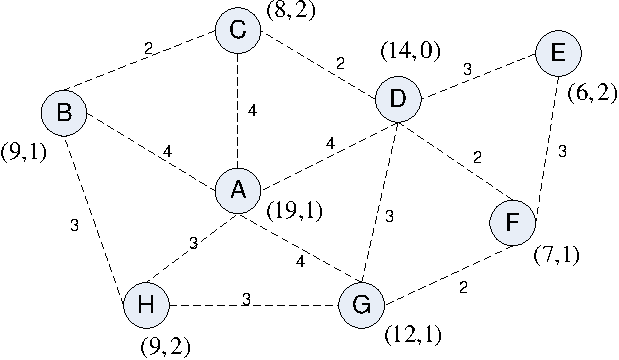
\includegraphics[width=0.6\linewidth]{figure1.pdf}
% 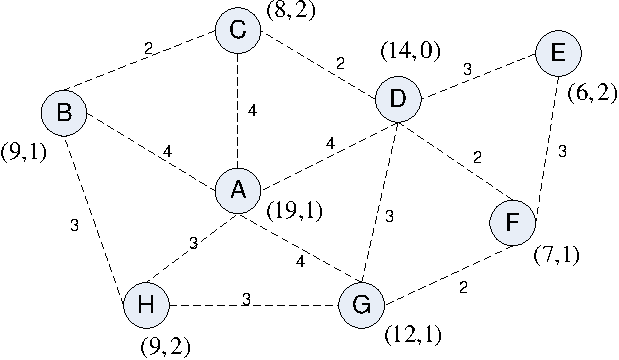
\includegraphics{figure1.pdf}
	\caption{Connectivity graph and the connectivity vector $\{D_i, G_i\}$ on each node. The available channels sensed by each CR node are: $V_A=\{1,2,3,4,5,6,10\}, V_B=\{1,2,3,5,7\}, V_C=\{1,3,4,10\}, V_D=\{1,2,3,5\}, V_E=\{2,3,5,7\}, V_F=\{2,4,5,6,7\}, V_G=\{1,2,3,4,8\}, V_H=\{1,2,5,8\}$. Dashed lines indicates two end nodes are within transmission range of each other. Each edge is labelled by the number of common channels between the two ends.}
	\label{fig1}
\end{figure}

The algorithm of phase I can be sketched like this: cluster heads are determined firstly, accordingly clusters are formed with cluster head's neighbourhood.

\subsubsection*{Determining Cluster Heads}
In this phase, each CR node decides whether it is cluster head by comparing relevant metrics with its neighbours.
Briefly speaking, the CR node which has the biggest \textit{individual connection degree} in its neighbourhood excluding already decided cluster heads becomes cluster, \ie CR node $i$ becomes cluster head if $D_i<D_k, \forall k\in Nb_i\setminus CHs$ ($CHs$ donate the cluster heads existing in $Nb_i$).
If there is another CR node $j$ in its neighborhood has the same \textit{individual connection degree}, \ie $D_j = D_i$, furthermore $D_j < D_{k}, \forall k\in Nb_j\setminus \{CHs\cup i\}$, then the node out of $\{i, j\}$ with higher \textit{social connective degree} becomes cluster head, and the other one becomes member of it. 
If $G_i = G_j$ as well, node ID is used to break the tie, \ie the one with smaller node ID takes precedence and becomes cluster head.
%This algorithm is contradictory to intuition by choosing the node with smallest $D_i$ as cluster head.
%The reason is that, by deciding cluster head in this way, the CR node with bigger $D_i$ will locate at the edge of clusters, and as they have higher \textit{Individual Connection Degree}, they are more likely to be integrated into one certain cluster, thus less singleton clusters are formed.

The pseudo code of phase I of clustering is in Algorithm~\ref{alg0}.
\begin{algorithm}              % enter the algorithm environment
\caption{Cluster head determination and cluster formation}          % give the algorithm a caption
\label{alg0} 
\DontPrintSemicolon
\SetAlgoLined
\KwIn{Unclustered CR node $i$ which is aware of $D_j$ and $G_j$, $j\in Nb_i$, and the ID of CRs which have be decided to be cluster heads, $ID_{CH}$, $CH\in Nb_i$. Empty sets $\tau_1,\tau_2,\tau_3,\tau_4,\tau_5$}
\KwResult{Whether or not $i$ is cluster head}
\For{CR node $j\in Nb_i\setminus CHs$}{
\eIf{$D_i==D_j$}{
	$\tau_1\leftarrow j$
	}
	{\If{$D_j < D_i$}{
		$\tau_2\leftarrow j$
		}
	}
	}
\uIf{$\tau_2 \neq \emptyset$}{
	$i$ is not CH; break;
	}
\uElseIf{$\tau_1$ is $\emptyset$}{
	$i$ is CH; break;
	}
\Else{ 	
\tcc*[r]{$\tau_1 \neq \emptyset, \tau_1 == \emptyset$}\mbox{}
	\For{$\forall k \in \tau_1$}{
	\If{$\nexists m\in Nb_k\setminus CHs$, such that $D_m < D_k$ }{
		$\tau_3 \leftarrow k$
		}
	}
	\eIf{$\tau_3$ is $\emptyset$}{
		$i$ is CH;break;
		}{
		\For{$\forall n\in \tau_3$}{
			\eIf{$G_n > G_I$}{
				$\tau_4 \leftarrow n$}{
				\If{$G_n == G_i$}{
				$\tau_5 \leftarrow n$
				}
			}
			}
		\uIf{$\tau_4 \neq \emptyset$}{
			$i$ is not CH;break;
			}
		\uElseIf{$\tau_4$ is $\emptyset$ and $\tau_5 \neq \emptyset$}{
		\If{$ID_i < ID_r, \forall r\in \tau_5$}{$i$ is CH;break;}	
		}
		\Else{$i$ is CH;break;\tcc*[r]{$\tau_4$ and $\tau_5$ are $\emptyset$}}
	}
}
\If{$i$ is cluster head}{
	$D_j, j\in Nb_i\setminus CHs$ is changed as a big positive value $M$;
	}
\end{algorithm}


\subsubsection*{Initial Cluster Formation}
After deciding itself being cluster head, CR node broadcasts to notify its neighbours on control channel, meanwhile, $i$'s initial cluster is formed immediately, which is $i$'s neighborhood except for those nodes which have become cluster heads, \ie $C_i=(Nb_i\setminus CHs)\cup i$.
It is possible that the formed cluster doesn't poses inner common channel, this can be handled in the following way. 
As smaller cluster size increases the number of common channels within the cluster, certain nodes are eliminated until there is at least one common channel.
The elimination of nodes is performed according to an ascending list of nodes sorted by their number of common channels with the cluster head, which means, the cluster member which has the least common channels with the cluster head will be excluded first.
If there are nodes having the same number of common channels with cluster head, the node whose elimination brings in more common channels will be excluded.
If this criterion meets a tie, the tie will be broken by deleting the node with smaller ID.
It is possible that the cluster head excludes all its neighbours and resulting itself to be the cluster.
%At the end of this procedure every formed cluster has at least one common channel.
Figure~\ref{fig1} depicts an example how CR nodes decide cluster heads. 
Node $B$ and $H$ have same individual connection degree, $D_B=D_H$, but as $G_H=2>G_B=1$, node $H$ becomes cluster head.
In Figure \ref{fig1}, the cluster $C_H$ is $\{H, B, A, G\}$.

As to the nodes eliminated in this procedure, they become either cluster heads or get included into other clusters later on, which is addressed in the following. 

After receiving the notification from a cluster head, a CR node is aware it is one member in a cluster, then the CR user changes its individual connection degree to be a big positive value $M$ (can be regarded as a positive infinite value), which is bigger than all the possible individual connectivity degrees in the CR network.
Then this CR user broadcasts this new individual connection degree to all its neighbours. 
If a CR node $i$ is associated to multiple clusters, $D_i$ is still set to $M$. %Note here that connectivity degree on cluster head will still be the actual value.% The value will expire after some duration and is changed later on back to the original value. 
When the cluster member is excluded from the cluster, its individual connection degree is restored to the original value which is further broadcast to its neighbours.
The purpose of manipulation on individual connection degree is to make the CR nodes out side this cluster possible to become cluster heads, so that every CR node either becomes cluster head or a member of at least one cluster.
The final states of all the CR users in the CRN are described in the following theorem.
%This judgement is conducted periodically, and phase I ends after every node ascertains it is cluster head or not.
\begin{lemma}
\label{clustering:lemma}
Every node in CRN will be included into at least one cluster in phase I in finite steps.
\end{lemma}

\begin{proof}
To see this, assume there are some nodes not assigned to any cluster and node $\alpha$ is one of them. As node $\alpha$ is not contained in any cluster, there must be at least one node $\beta\in Nb_\alpha$, with $D_{\beta} < D_{\alpha}$. Thus, node $\beta$ has at least one neighbouring node $\gamma$ with $D_{\gamma}<D_{\beta}$, and this series of nodes with monotonically decreasing $D_i$ might continue but finally ceases because the total number of nodes is limited. Now we find the last node $\omega$ in this series, because $\omega$ is the end node and does not have neighbouring nodes with smaller connectivity degree $D$, so $\omega$ will become a cluster head and embrace all its one-hop neighbours, including the node before it in the node series (here we assume that every new formed cluster has common channels). After that, the node recruited into cluster will set its connectivity degree $D$ to $M$, which enables the node further down in the list to become a cluster head. In this way, all the nodes in the series are included in at least one cluster in an inverse sequence. This clearly contradicts the initial assumption and proves the claim stated above. The proof implicitly shows that, within $\vert I \vert$ steps, all nodes will become a part of certain clusters and so phase I converges.
\end{proof}
According to Lemma~\ref{clustering:lemma}, we can assign reasonable amount of time for phase I to complete.
The pseudo code for cluster head to obtain at least one common channel is shown in Algorithm~\ref{alg_size_control_available_CCC}.



\subsubsection*{Cluster Size Control in Dense CRN}
\label{cluster_pruning}
In the introduction section, we have stated that cluster size should be given consideration to justify the pursuing of robust clusters, here we illustrate the pressing necessity to control cluster size when CRN becomes dense via theoretical analysis and simulation, and provide solution to it.

Assume CR nodes and primary users are evenly distributed and primary users occupy the licensed channels randomly, \ie both CR nodes density and channel availability in the CRN is homogeneous.
Based on Algorithm~\ref{alg0}, cluster heads are the CR nodes which poses the biggest individual connection degree in their neighborhood, and they are surrounded by CR nodes.
In contrast, CR nodes residing on edge are unlikely to become cluster heads as their neighbourhoods are only half the nodes locating away from edge.
The clusters formed are the neighborhood of cluster heads, which is decided by the transmission range and network density.
When this CRN becomes extremely dense, assume one cluster is formed by CR node $i$, based on the rule for cluster head selection Algorithm~\ref{alg0}, the nearest cluster head generated could locate just outside the neighborhood or transmission range of $i$, which is as Figure~\ref{clusters_denseNetwork} shows.
%
In the figure, black dots represent cluster heads, the circles denotes the transmission ranges of those cluster heads.
Cluster members are not shown in the figure.
%Circles represent the transmission range of cluster head, within which CR nodes are absorbed in cluster.
\begin{figure}[h!]
  \centering
  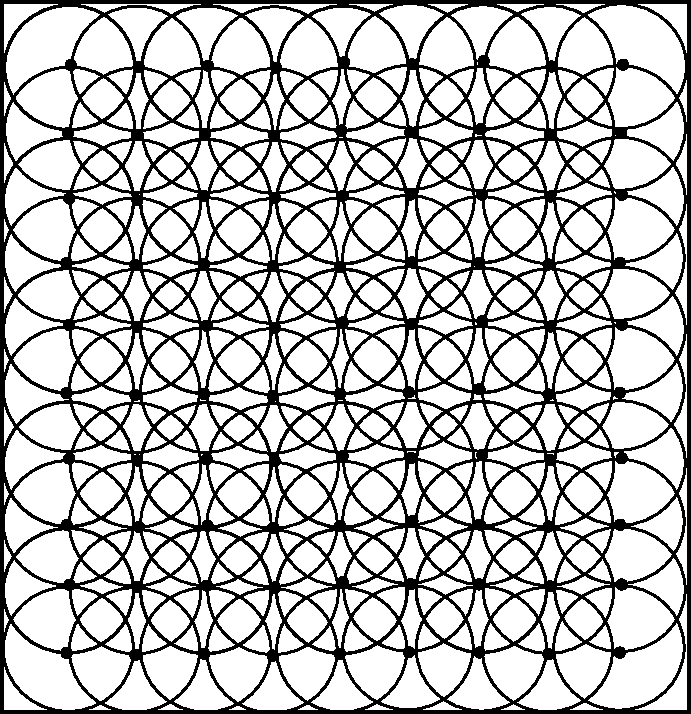
\includegraphics[width=0.5\linewidth]{clusters_denseNetwork_2.pdf}
  \caption{Clusters formation in extremely dense CRN. Black dots are cluster heads, cluster members are not drawn.}
  \label{clusters_denseNetwork}
\end{figure}
Let $l$ be the length of side of simulation plan square, and $r$ be CR's transmission radius.
Based on the aforementioned analysis and geometry illustration as Figure~\ref{clusters_denseNetwork}, we give an estimate on the maximum number of generated clusters as $l^2/r^2$.

Now we show the estimation is valid with simulation.
We distribute CR users and primary users randomly on a square plan, and set $r=10, l=50$.
Network density is increased by adding more CR users.
For each network scale, simulation is run for 50 times.
%We now have a look at how does the network density affect the cluster size when the transmission range is constant.
%This implicates when the cluster size is decided by the density of the network.
%As to SOC, the membership of one cluster is decided after a complex process, and the cluster size is roughly the same with one neighborhood.xxxx
%We can see from the example that although two neighbouring clusters can overlap greatly with each other, no cluster head will be covered by other clusters.
Figure~\ref{number_clusters_scale} shows the number of formed clusters.
With the increase of CR users in the network, network density increases linearly (see the right hand side Y axis, which indicates the number of neighbours.), and the number of formed clusters also increases and approaches to the the upper bound of 25 which complies with the estimation.
The confidence rate is 95\% in the figure.

\begin{figure}[ht!]
  \centering
  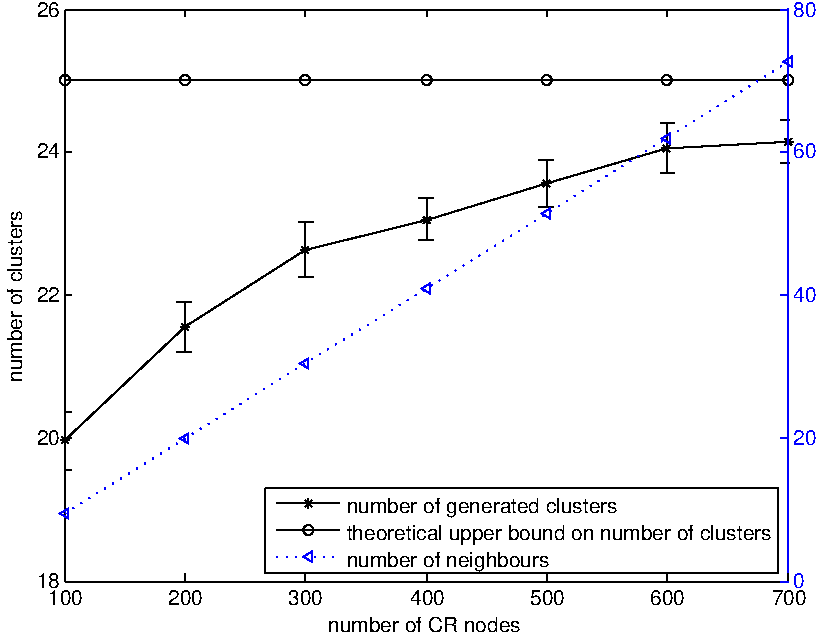
\includegraphics[width=0.67\linewidth]{number_clusters_upperBound.pdf}
  \caption{Number of clusters formed}
  \label{number_clusters_scale}
\end{figure}

Both the analysis and simulation show that with the increase of network density, the cluster size also increases.
In case of dense network where cluster size is big, there will be heavy burden on cluster heads to manage their clusters, which is a challenge for resource limited cluster heads, besides [xxxxx].
As a result, certain measures are needed to prevent the network size to increase with the increasing network density.
This task falls on cluster head.
To control cluster size, cluster heads prune their cluster members if sizes are greater than the desired size $\delta$.
Given desired size as $\delta$, cluster head excludes members sequentially, whose absence leads to the maximum increase of common channels within the cluster.
This process ends when the size of resultant cluster is at most $\delta$ and at least one CCC is available.
This procedure is similar with guaranteeing CCC available to be available in cluster, thus the algorithm is also given in Algorithm~\ref{alg_size_control_available_CCC}.


\begin{algorithm}               % enter the algorithm environment
\caption{ICC guarantee and cluster size control by cluster head}          % give the algorithm a caption
\label{alg_size_control_available_CCC}
\DontPrintSemicolon
\SetAlgoLined
\KwIn{Initial cluster formed, empty sets $\mathcal{T}_1, \mathcal{T}_1$}
\KwOut{cluster has at least CCC, and satisfies the requirement on cluster size}
\tcc*[r]{When available CCC is to be guaranteed, execute line 1, when cluster size control is conducted, execute line 2}
\textbf{while} $V_C =\emptyset$ \textbf{do}\\
\While{$|C|>\delta+1$}{
calculate $\lambda = \min_{i\in C, i\neq H_C}(|K_{H_C}\cap K_i|)$;\\
	\For{each $i\in C\setminus H_C $}{
	\If{$|V_{H_C}\cap V_i| ==\lambda$}{$\mathcal{T}_1\leftarrow i$}
	}
\eIf{$|\mathcal{T}_1|==1$}{delete node $i$ from $C$;\\break;}
{
calculate $\mu= \Max_{i\in \mathcal{T}_1}(|\cap_{j\in C\setminus i} V_j|-|\cap_{j\in C} V_j|)$;\\
	\For{each $i\in \mathcal{T}_1$}{
	\If{$|\cap_{j\in C\setminus i} V_j|-|\cap_{j\in C} V_j| ==\mu$}{$\mathcal{T}_2\leftarrow i$}
	}
\eIf{$|\mathcal{T}_2|==1$}{delete node $i$ from $C$;\\break;}
	{
	delete $i\in \mathcal{T}_2$, which has the highest ID;
	}
}
}
\end{algorithm}

%Figure~\ref{fig2} shows the clusters formed in the example in Figure~\ref{fig1} when the desired cluster size is 3. 

%Especially, it forster the connectivity between the clusters. It can do so, as the nodes with larger connectivity degree are not cluster heads but members. 
%As basin nodes have smaller $d_i$ compared with its cluster members, and many of the cluster members locate between the basin node and neighbor clusters,  %the bigger $d_i$ with bigger robustness of Social Connection, i.e, with bigger $d$ are located around cluster heads, 
%After clusters are formed, with aid of \textit{control channel rotation scheme} proposed in \cite{Lazos09}, intra and inter cluster communication is conducted and for each debable node (XXX Debatable nodes are not defined yet), the membership and channel availablity of the clusters concluding it is known. 


\begin{figure}[ht!]
  \centering
  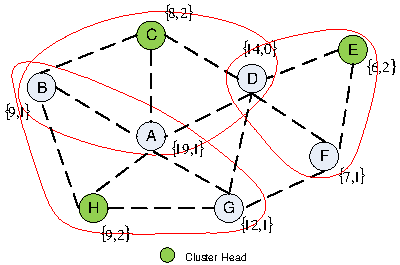
\includegraphics[width=0.6\linewidth]{figure2.pdf}
  \caption{Clusters formation after the first phase of ROSS. Some nodes remain debatable nodes after the first phase.}\label{fig2}
\end{figure}


\subsection{Phase II - Membership Clarification}
%\subsubsection*{Problem Description}
After applying ROSS phase I on the example in Figure~\ref{fig1}, we get the clusters shown in Figure~\ref{fig2}.
We notice there are several nodes, \ie $A, B, D$, are included into more than one cluster. 
We refer these nodes as \textit{debatable nodes} as their cluster affiliations are not clear, and the clusters which include debatable node $i$ are called \textit{claiming clusters} of node $i$, and are represented as $S_i$.  
Actually, debatable nodes extensively exist in CRN with larger scale.
Figure~\ref{percentage_overlapping_node} shows the percentage of debatable nodes increases with the scaling of CRN network.

Debatable nodes should be exclusively associated with one cluster and removed from the other claiming clusters, this procedure is called cluster membership clarification.
We will introduce the solution for cluster membership clarification in the following.

\begin{figure}[ht!]
  \centering
  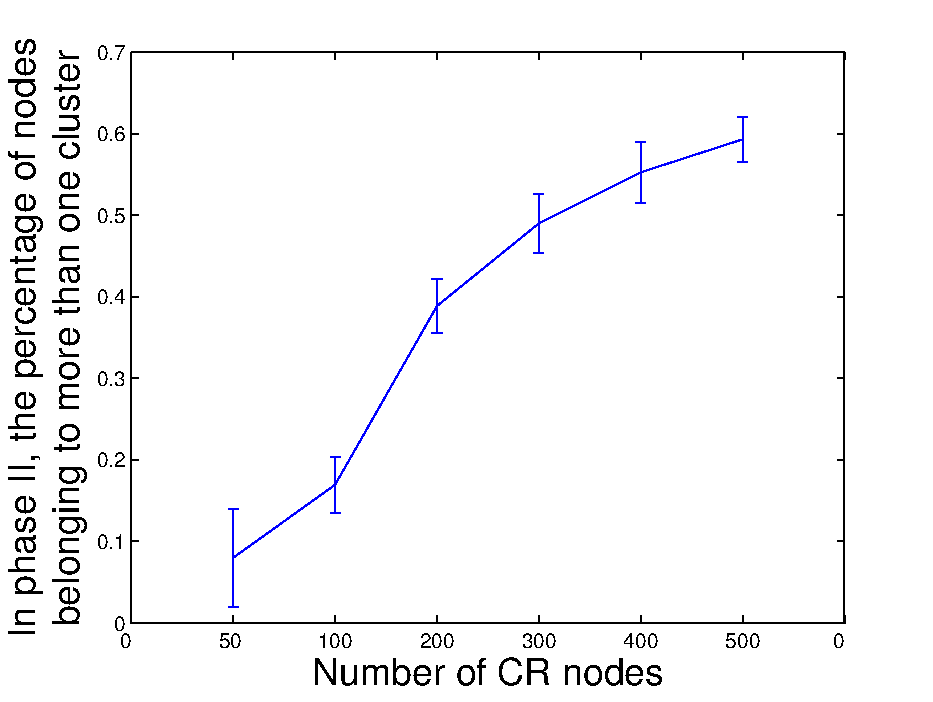
\includegraphics[width=0.6\linewidth]{percentage_overlapping_node.pdf}
  \caption{Clusters formation after the first phase of ROSS. Some nodes remain debatable nodes after the first phase.}\label{percentage_overlapping_node}
\end{figure}



%In the second phase of ROSS, debatable nodes will chose only one cluster to reside.

%In particular, the un-affiliation of one debatable nodes from a cluster increasing the set $K_C$ of ICCs of cluster $C$ (at the cost of potentially decreasing $R_C$, the set of OCCs).

%\newtheorem{observation}{Observation}
%\label{observation}
%\begin{observation}
%If the number of nodes within a cluster decreases, the number of common channels will increase or keep constant.
%\end{observation}
%
%\begin{proof}
%Contradiction, To be continued
%\end{proof}
%From observation 1 we know that the procedure of membership clarification will increase the set of common channels for some clusters and accordingly strengthen the robustness of intra connectivity. 

% % % % %	dependancy!
%An debatable node belongs to multiple clusters, and in the same time, it is possible that several debatable CR nodes locate within one same cluster. %Each debatable node tries to increase the sum of ICC of the clusters which it belong to. More specifically, 
%For a debatable node $i\in S_i$ after phase I, as to clarify its membership, it will choose one cluster $C\in S_i$ to stay and withdraw from the other clusters in $S_i$ with the consideration of increasing ICCs within $S_i$ by the largest margin. 

\subsubsection*{Distributed Greedy Algorithm (DGA)}
%Debatable node $i$ is aware of all its claiming clusters in $S_i$. 
After Phase I, debatable nodes, \eg $i$ needs to decide which cluster $C\in S_i$ to stay, and leaves the others.
The principle for debatable node $i$ to choose one claiming cluster is to result in the greatest increase of common channels in all its claiming clusters.
%The set of available channels of one cluster are known by the debatable nodes which locate in that cluster. %this is finished 
Node $i$ communicates with all the cluster heads whose clusters are in $S_i$, and is aware of the vector of common channels of the claiming clusters, then $i$ is able to calculate how many more common channels in one certain claiming cluster if $i$ leaves that cluster.
Based on this calculation, $i$ decides in which claiming cluster to stay and leaves the other claiming clusters.
If there exists one cluster $C\in S_i$, by leaving from which the clusters in $S_i$ obtain the minimum increased common channels than leaving any other claiming clusters, then $i$ chooses to stay in cluster $C$.
When there comes a tie in terms of the increase of common channels among multiple claiming clusters, $i$ chooses to stay in the cluster whose cluster head shares more common channels with $i$.
In case there are multiple claiming clusters demonstrating the same on the aforementioned metrics, node $i$ chooses to stay in the smallest claiming cluster.
IDs of cluster heads will be used to break tie if the previous rule doesn't decide on the unique cluster to stay.

Algorithm for debatable node $i$ to decide which claiming cluster to stay is described as Algorithm~\ref{alg4}.
To conduct Algorithm~\ref{alg4}, debatable node $i$ needs to know the necessary information about its claiming clusters, \ie $V_C$, $V_{H_C}$, $|C|$,$C\in S_i$, which are respectively the set of available channels in $C$, the set of available channels on $C$' cluster head $H_C$, and $C$' cluster size.
Node $i$ decides which cluster to stay based on Algorithm~\ref{alg4}, then notifies all its claiming clusters, and retrieves the updated information of the necessary information $V_C$, $V_{H_C}$, $|C|$, where $C\in S_i$.

\begin{algorithm}               % enter the algorithm environment
\caption{Debatable node $i$ decides its affiliation, chooses one claiming cluster to stay and leaves all the other claiming clusters}          % give the algorithm a caption,  cluster to settle
\label{alg4}
\DontPrintSemicolon
\SetAlgoLined
\KwIn{all claiming clusters $C\in S_i$}
\KwOut{one cluster $C$}
calculate $\lambda = \Min_{C\in S_i}(|K_{C\setminus i}|-|K_C|)$;\\
define set $\mathcal{C}_1$;\\	
	\For{each $C\in S_i$}{ 
	\If{$|K_{C\setminus i}|-|K_C| ==\lambda$}{$\mathcal{C}_1\leftarrow C$}\tcc*[r]{metric is the increase of CCCs due to $i$' departing}
	}
\eIf{$|\mathcal{C}_1|==1$}{choose cluster $C$;\\break;}
{
calculate $\mu= \Max_{C\in \mathcal{C}_1}(V_{H_C}\cap V_i)$;\\
define set $\mathcal{C}_2$;\\	
	\For{each $C\in \mathcal{C}_1$}{
	\If{$V_{H_C}\cap V_i ==\mu$}{$\mathcal{C}_2\leftarrow C$}\tcc*[r]{metric is the number of common channels between $i$ and cluster head of demanding cluster}
	}
\eIf{$|\mathcal{C}_2|==1$}{choose cluster $C$;\\break;}
	{
	calculate $\nu=\min_{C\in \mathcal{C}_2}|C|$;\\
	define set $\mathcal{C}_3$;\\	
		\For{each $C\in \mathcal{C}_2$}{
		\If {$|C|==\nu$}{$\mathcal{C}_3\leftarrow C$}	\tcc*[r]{metric is cluster size}
		}
	\eIf{$|\mathcal{C}_3|==1$}{choose cluster $C$;\\break;}
		{choose the $C\in \mathcal{C}_3$, which has the highest ID;
		}
	}
}
Node $i$ notifies $H_C$ which is cluster head of $C$ of its affiliation decision, cluster $C$ then accepts it.

\end{algorithm}



This procedure raises the concern on infinite chain effect that debatable nodes update their choices based on other debatable nodes' choices, and never cease.
Assume debatable node $i$ locates in one cluster $C\in S_i$, and $C$ could have more than one debatable node except for $i$.
Let $i$ our of $C$'s debatable nodes to make decision on the cluster to stay first.
Then the choices of those debatable nodes except for $i$ change $C$'s membership, which possibly further triggers node $i$ to alter its previous decision.
%To maximize the increase of common channel in clusters in $S_j$, $j$ either stays in $C$, or leaves cluster $C$ and stay another cluster in $S_j$.
%$j$'s decision changes $C$'s membership, which will affect $i$'s decision.
%Assume $i$ makes decision before $j$ and chooses to stay in $C$, as which brings the most common channels in $i$' claiming clusters, and then it is $j$' turn to choose cluster.
%If $j$ leaves $C$, the smaller cluster $C$ will possibly make $i$ to leave it and join another cluster.
%and the choice of $j$ to stay in $C$ or not possibly changes $C$'s membership and  which potentially further triggers node $i$ to alter its previous decision. 
Thus, we must answer this question raised when implementing ROSS-DGA.
%, and if it converges, how good such a distributed scheme performs. 
In the following we show that the process of membership clarification can be converted to a congestion game, and a equilibrium state is reached after a finite number of best response updates.

\subsubsection*{Bridging ROSS-DGA with Congestion Game}
In this part, we illustrate that when debatable nodes decide on the exclusive clusters to stay, in particular, the 
To formulate the problem of membership clarification for the debatable nodes in the context of a game, we look at the problem from a different perspective. 
In the new perspective, the debatable nodes are regarded as isolated and don't belong to any cluster, which means the clusters they used to belong to become their neighbouring clusters. 
Then as to each debatable node, the previous problem to decide which clusters to leave becomes a new problem that which cluster to join.
In this new problem, debatable node $i$ (note now $i\notin S_i$) chooses one cluster $C$ out of $S_i$ to join if the decrement of common channels in cluster $C$ is the  %(among the clusters set $CS$, but now, each cluster $C\in CS$ does not conclude $i$) 
smallest in $S_i$, and the decrement of number of ICC in cluster $C$ is $\sum_{C\in S_i}\Delta\vert K_C \vert=\sum_{C\in S_i}({\vert K_{C} \vert-\vert K_{C\cup i} \vert})$. %  $c'$ is the cluster after implementing the strategy, and $c$ is the original cluster.
The relation between debatable nodes and claiming clusters is shown in Figure~\ref{debatable_nodes_claiming_cluster}.
\begin{figure}[ht!]
  \centering
  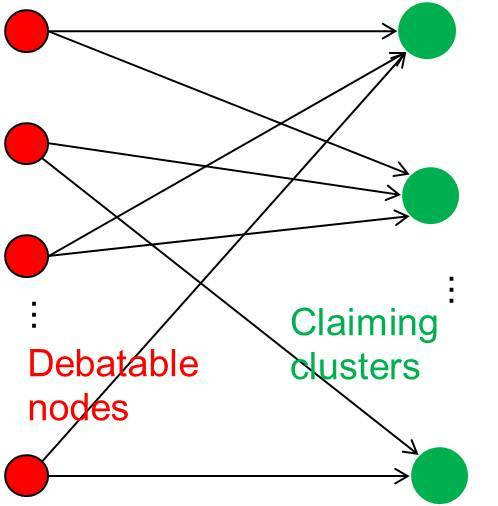
\includegraphics[width=0.30\linewidth]{singletongame.pdf}
  \caption{debatable nodes and claiming clusters}
  \label{debatable_nodes_claiming_cluster}
\end{figure}

In the following, the debatable nodes constitute the players, and the 
we show that the decision of debatable nodes to clarify their membership can be mapped to the behaviour of the players in a \textit{player-specific singleton congestion game} when proper cost function is given.

The game to be constructed can be represented by a 4-tuple $\Gamma=(\mathcal{P},\mathcal{R},(\sum_i)_{i \in \mathcal{N}},\Delta\vert K^i_C \vert)$, where elements in $\Gamma$ are given as below,
%To make the model of this game more clear, we make some change to our original problem. Previously, the nodes in overlapping areas belong to more than one cluster, and our scheme is to remove them out of some clusters to increase the set of common channels within the cluster form which the mode leave. In the new model, we assume all the nodes in overlapping nodes don't belong any cluster and the problem become into how do these nodes decide which cluster to join.

%The components of the game are listed as follows,

\begin{itemize}
%	\item $\mathcal{D}=\left\{1,\ldots,n\right\}$, the set of players (debatable nodes).
	\item $\mathcal{P}$, the set of players of the game, which are the debatable nodes after phase I in our clustering problem.
%	\item $\mathcal{R}=\left\{1,\ldots,m\right\}$, the set of resources which player can choose, which are all the clusters in our model.
	\item $\mathcal{R} = \cup S_i, i\in \mathcal{P}$, denotes the set of resources for players to choose, $S_i$ is the set of claiming clusters of node $i$. $\mathcal{R}$ is the set of claiming clusters after phase I in our clustering problem.
	\item As to the strategy space $\sum_i$ of player $i\in \mathcal{N}$, there is $\sum_i \subseteq 2^{\left[S_i\right]}$. As one debatable node is supposed to choose one claiming cluster in our problem, thus only one resource is allocated for $i$, accordingly this congestion game is a singleton game.
	%when $i$ makes decision, only one resource (one claiming cluster) from the allowed resources is allocated.
	
	%\item We denote by $\mathcal{S}=\left(\mathcal{S}_1,\ldots,\mathcal{S}_n\right)\in \sum_1\times \cdots\times\sum_n$ the state of game where player $i$ plays strategy $\mathcal{S}_i\in \Sigma_i$.
	
	\item %For the clusters which are possible destination of debatable nodes, the decrement of common channels caused by different debatable node' join can be different because of the heterogeneity of channel availability within itself and on the debatable nodes. %furthermore, the sequence of debatable node's join can also alter the decrement. 
	The utility (cost) function $f(C)$ of resource $C\in R$, (or to say $f(r)$ of resource $r \in \mathcal{R}$) is $\Delta\vert K^i_C \vert$ which represents the decrement of ICCs in cluster $C$ caused by debatable node $i$' joining in it.
	As to cluster $C\in S_i$, the decrement of ICCs caused by enrolment of debatable nodes is $\sum_{i:C\in S_i, i\rightarrow C} \Delta\vert K^i_C \vert$. 
$i\rightarrow C$ means $i$ joins in cluster $C$.
Obviously this function is non-decreasing with respect to the number of nodes joining in cluster $C$.
	
The utility function is not purely decided by the number of players (debatable nodes) as that in a canonical congestion game, as in this game the channel availability on debatable nodes is different.
Given two same sized groups of debatable nodes, when the nodes are not completely the same (neither are the channel availabilities on these nodes), the cost happened on one claiming cluster could be different if the two groups of debatable nodes join in that cluster respectively.
%In a canonical congestion game, the cost (or pay off) is function of only the number of players occupying the resource, and is mono-
%In this new game, the cost function 
Hence, this game is called player specific.
In this game, every player greedily updates its strategy (choosing one claiming cluster to join) if joining in a different claiming cluster minimizes the decrement of ICCs $\sum_{i:C\in S_i} \Delta\vert K^i_C \vert$, player's strategy in the game is exactly the same with the behaviour of debatable node in membership clarification phase, which is described by Algorithm~\ref{alg4}.


%	\item The Rosenthal's potential function \cite{Rosenthal} of this congestion game is given by:
%	\begin{equation*}
%	\phi(S)=\sum_{C\in\mathcal{R}} \sum_{i:C\in S_i} \Delta\vert K^i_C \vert   	
%   	%\sum_{i=1}^N \Delta^{i}_{p}(S)=\sum_{i=1}^N \sum_{r\in S_i}\Delta^{i}_{r}(t)	
%  	% \Delta =\sum_{i=1}^N w_i (x_i - \bar{x})^2 .
%	\end{equation*}
%All the players in this game greedily update their strategy to minimize the potential function (congestion), this process is exactly the same with the network behaviour under \textit{Distributed Greedy Algorithm}. 

%	\item It is an asymmetric game because the sets of strategies shared by different players are different.
%	\item The total cost is: 
%\begin{equation*}
%   \sum_{i=1}^N \Delta^{i}_{p}(S)=\sum_{i=1}^N \sum_{p\in s_i} \Delta^{i}_{p}(n_p(S))
%  % \Delta =\sum_{i=1}^N w_i (x_i - \bar{x})^2 .
%\end{equation*}

%This is the global objective we want to minimize.
\end{itemize}

%Singleton congestion game is a special type of matroid game~\cite{Milchtaich1996111,}. 
%It is known that player-specific matroid congestion game admit pure equilibrium, 

As to singleton congestion game, there exists pure equilibria which can be reached with greedy update~\cite{Ackermann06purenash}.


%and the number of steps towards \textit{Nash Equilibrium} is upper-bounded\footnote{Here we present this with modifying the original conclusion in \cite{Ackermann06purenash} according to our model.} by $ n^2\cdot m $. In our context, $n$ is the number of debatable nodes, $m$ is number of clusters in CRN, %$rk(\Gamma)$ of the matroid  is the cardinality of the maximal independent sets, which is 1 in the case of singleton game, 
%so the total time complexity to achieve the \textit{Nash Equilibrium} using greedy approach is 	.
%%(XXX Just mention after this complexity result the relationship to the system mdeol XX)
%This is upper-bounded (in the worst case) by $O(\vert I\vert^3)$. 
Based on above model and analysis, phase II converges is Algorithm~\ref{alg4} is run by debatable nodes. 
%Although the game version of DGA can achieve \textit{Nash Equilibrium}, the whole scheme can possibly obtain sub-optimal result.    %, furthermore,this stable state is a local minimum of the global decrement function.
%\todo[inline]{The number of steps, or the upper bound of steps in convergence needs a formal proof}

\subsubsection*{Distributed Fast Algorithm (DFA)}
The complexity of DGA is quite large recalling that the formation of clusters takes at most $|I|$. Here we propose a faster algorithm DFA which is especially suitable for CRN where channel availability might change dynamically and re-clustering is possible. %Note that the algorithm is based on the problem description of phase II. 
In DFA, each debatable node executes only one iteration of Algorithm~\ref{alg4} (by setting 'the current value' in Line 14 to zero). Every cluster includes all its debatable nodes, thus the membership is static and debatable nodes can make decisions simultaneously without considering the change of membership of its claiming clusters. For example, for node $A$ in Figure \ref{fig2}, the membership of cluster $C_C, C_H\in S_A$ are $\{A,B,C,D\}$ and $\{A,B,H,G\}$ respectively. 

The two possible strategies of node $A$'s clarification is illustrated in Figure \ref{fig3}. In Figure \ref{AinC}, node $A$ staying in $C_C$ and leaving $C_H$ brings 2 more ICC in $S_A$, as it is more than that brought by another strategy showed in \ref{AinH}, $A$'s membership is clear. After the decisions made similarly by the other debatable nodes $B$ and $D$, the final clusters formed are shown in Figure~\ref{fig4}.

%Using DFA in phase II, the time complexity is decreased drastically to 1. Thus, the total complexity of ROSS-DFA is $|I|$, while, ROSS-DGA's complexity is $|I|^3$ in the worst case.


\begin{figure}[ht!]
\centering
\subfigure[Node A stays in cluster $C_C$, quits $C_H$, $\Delta\vert K_{C_C}\vert+\Delta\vert K_{C_H}\vert=2$]{
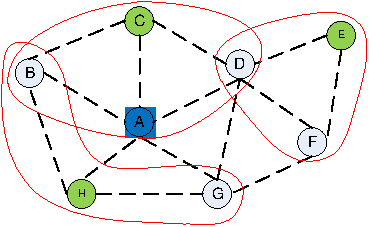
\includegraphics[width=0.435\linewidth]{figure4AinC.pdf}
\label{AinC}
}
\subfigure[Node A stays in cluster $C_H$, quits $C_C$, $\Delta\vert K_{C_C}\vert+\Delta\vert K_{C_H}\vert=1$]{
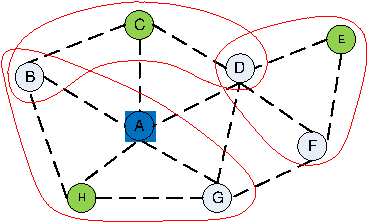
\includegraphics[width=0.435\linewidth]{figure4AinH.pdf}
\label{AinH}
}
\caption[]{Membership clarification: possible cluster formations decided by node A's different choices} %\subref{node A in $C_C$}, \subref{node A in $C_H$}}
\label{fig3}
\end{figure}

\begin{comment}
As an example, when node A comes to decide which cluster to stay, the memberships of relevant clusters, like $C_C$ and $C_H$, are $\{C,B,D,A\}$ and $\{H,B,G,A\}$ respectively. Before the other two debatable nodes B and D making their belonging clear, cluster $C_C$ and $C_H$ have them in the same time. So node A can decide which cluster to belong to without considering other debatable nodes' action. There are two strategies for node A, which is illustrated in Figure \ref{fig3}. Because staying in cluster $C_C$ brings in more common channels within relevant clusters, node A finally choose cluster $C_C$ to stay and caveat from cluster $C_H$. The membership of $C_H$ is updated in the same time. Node B and D undertake the same process and the clusters are formed finally as Figure \ref{fig4} shows.

Because debatable nodes can conduct membership clarification abased on static membership information of relevant clusters, thus no iteration happens in this process. The time complexity of this algorithm is only decided by the number of debatable nodes, which is maximal $O(\vert I\vert)$. 

As an example, when node A comes to decide which cluster to stay, the memberships of relevant clusters, like $C_C$ and $C_H$, are $\{C,B,D,A\}$ and $\{H,B,G,A\}$ respectively. Before the other two debatable nodes B and D making their belonging clear, cluster $C_C$ and $C_H$ have them in the same time. So node A can decide which cluster to belong to without considering other debatable nodes' action. Figure \ref{AinC}. Because staying in cluster $C_C$ brings in more common channels within relevant clusters, node A finally choose cluster $C_C$ to stay and retreat from cluster $C_H$. The membership of $C_H$ is updated in the same time. Node B and D undertake the same process and the clusters are formed finally as Figure \ref{fig4} shows.
\end{comment}


\begin{figure}[ht!]
  \centering
  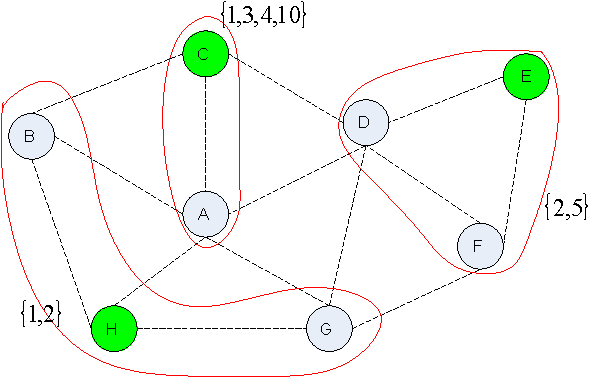
\includegraphics[width=0.5\linewidth]{final_clustering_ross.pdf}
  \caption{Final formation of clusters, common channels for each cluster is shown.}
  \label{fig4}
\end{figure}


\newpage
\section{Centralized Clustering Scheme}
\label{centralized_scheme}

%paper given by james is useful which provides a survey from the perspective of wsn!


%\todo[inline]{check}
The centralized clustering scheme aims to form clusters with certain sizes, meanwhile the total number of common channels of all clusters is maximized.
In the following, we refer this problem as \textit{centralized clustering} for short, and the problem definition is as follows, 


\begin{mydef}
\label{def_centralized_clustering}
\textit{Centralized clustering in CRN.}

Given a cognitive radio network $\mathcal{N}$ where nodes are indexed from 1 to $N$ sequentially.
Based on certain correlation, certain secondary users constitute one cluster $C$.
$1\leq |C| \leqslant k$ where $|C|$ is size of cluster $C$ and $k$ is positive integer.
We name the collection of such clusters as $\mathcal{S}=\{C_1, C_2,\ldots,C_{|\mathcal{S}|}\}$ (the subscript $i$ is the unique index of cluster in $\mathcal{S}$, not the ID of cluster head of relevant cluster), $\mathcal{S}$ has following properties: $\bigcup_{1\leq i \leq l} C_i = N$ and $V_{C_i}\neq \emptyset$ for any $i$ which satisfies $1\leq i \leq l$.

Following condition distinguish the centralized clustering problem discussed in this thesis.
The number of common channels is denoted as $f$ which is $|V_{C}|$ if $|V_{C}|>1$, and $f=0$ if $|V_{C}|=1$.
The question of this problem is to find a subcollection $\mathcal{S}' \subseteq \mathcal{S}$, so that $\bigcup_{C_j\in \mathcal{S}'} C_j = N$, and $C_j'\cap C_j =\emptyset$ for $C_j', C_j\in \mathcal{S}'$, so that $\sum_{C\in \mathcal{S}'} f$ is maximized.
% when $|C|>1$, and $f(\cdot)=0$ when $|C|=1$.
%As to $f(\cdot):z\rightarrow z$, under this problem setting, if only number of common channels are given consideration, only singleton clusters will be preferred, which contradicts to our goal of clustering CR nodes together, thus we choose $f(\cdot)= |V_{C}|\cdot |C|$, the product of number of common channels and cluster size.
The decision version of centralized clustering in CRN is to ask whether exist $\mathcal{S}'\subseteq \mathcal{S}$, so that $\sum_{C\in \mathcal{S}'} f \geqslant \lambda$ where $\lambda$ is a real number.% in stead of to maximize $\sum_{C\in \mathcal{S}'} f$.
\end{mydef}


%The decision version of \textit{weighted exact cover problem}: 
%Given an universe $U$, and collection $S=\{s_1, s_2, \ldots, s_m\}$ where each subset $s_i\subseteq U$ and is given a weight $w_i$, whether there exists a collection of subsets $\mathcal{C}$ and constant number $\lambda$, so that the union of $\mathcal{C}$ equals to $U$, $s_j\cap s_{j'} = \emptyset$ for different $j$ and $j'\in \{1,2,\ldots, m\}$, and $\sum_{i\in J} w_i \geq \lambda$.

In the following part of this section, we will discuss the complexity of centralized clustering problem and provide solution for it.
We put the definition of weighted k-set packing problem here as it will be used in the analysis on the complexity of our problem.

\begin{mydef}
\label{def_kset_packing}
\textit{Weighted k-set packing.} 

Given a set $\mathcal{G}$ which contains finite number of positive integers, and a collection of set $\mathcal{Q}=\{s_1,s_2,\cdots,s_m\}$, where for each element $s_r, 1\leq r \leq m$, there is $s_r\subseteq \mathcal{G}$, $ 1\leq|s_r| \leq k$, and $s_r$ has an associated weight which is positive real number.
The question is whether exists a collection $\mathcal{S}\subseteq \mathcal{Q}$, where $\mathcal{S}$ contains only disjoint sets and the total weight of sets in $\mathcal{S}$ is greater than $\lambda$.
Weighted k-set packing is NP-hard when $k\geqslant 3$.~\cite{Computers_a_Intractability}
\end{mydef}

\begin{theorem}
\label{theorem1}
CRN clustering problem is NP-hard, when the maximum size of clusters $k\geqslant 3$.
%Assume a CRN can be represented by a connected graph, and there is at least one common channel between any pair of neighbours, then forming at least two CR nodes into one cluster is NP-complete.
\end{theorem}

\begin{proof}
To see centralized clustering problem is NP-hard, we reduce the NP-hard problem \textit{weighted k-set packing} to it.
%, which means centralized clustering in CRN problem is as hard as weighted k-set packing to be solved.

To complete the reduction, we need to conduct following two steps:
\begin{itemize}
\item step 1: Show there exists a polynomial algorithm $\sigma$, by which any instance (\eg $\mathcal{S}$) of a weighted k-set packing can be transformed to instance $\sigma(\mathcal{S})$ for centralized clustering.
\item step 2: Show that $\mathcal{S}$ is a \textit{yes} instance of weighted k-set packing if and only if $\sigma(\mathcal{S})$ is an \textit{yes} instance for CRN clustering problem.
\end{itemize}

We continue using the notation introduced in problem definition.
Let set $\mathcal{G}$ contains $N$ positive integer numbers which are indexed from 1 to $N$ sequentially.
Assume one instance $\mathcal{S}$ of weighted k-set packing is a collection of disjoint sets $\mathcal{Q} = \{s_1, s_2,\cdots s_m\}$, each set is composed by certain amount of elements in $\mathcal{G}$.
$\omega$ indicates the weight for each set $s$, $\omega:\mathcal{S}\rightarrow \mathbb{Z}^{+}$.
%As the number of common channel of clusters is always integer
%give new weight to them in following way



The polynomial algorithm $\sigma$ consists of three transformations.
\begin{itemize}
\item In the first transformation, for each set $s_i$ of instance $\mathcal{S}$, the elements are duplicated, for instance, given $s_i=\{1, 4, 6\}$, the dummy set $s_i'$ is $\{1,1,4,4,6,6\}$.
By doing this, we obtain the dummy sets and constitute the dummy instance $\mathcal{S}'$ based on $\mathcal{S}$.
The purpose of this transformation is to eliminate the single element set in $\mathcal{S}$.
The weight of set is unchanged after this transformation, \ie $\omega(s_i)=\omega(s_i')$.
After this transmission, there is no set with only one element.
This transformation requires $\sum_{s_i \in \mathcal{S}} |s_i|$ steps.
\item In the immediate following second transformation, we transform the dummy instance $\mathcal{S}'$ to an instance for CRN clustering problem.
Given an instance $\mathcal{S}'$, we retrieve all the elements which appear in it, and map each of those elements into one CR node, \ie each integer corresponds to one CR node, particularly, that integer becomes the CR node's ID.
As to duplicated elements, we also map them into a CR node, thus there exist CR nodes with the same ID.
As a result, these CR nodes constitute a collection of CR nodes, but note that they have not constituted one CRN yet as there are not connections drawn among them.
Connections in CRN under this context is decided by physical conditions, which says the corresponding CR nodes have common channels and close enough to communicate with each other.
This transformation requires $2\cdot\sum_{s_i \in \mathcal{S}} |s_i|$ steps.
%We further assume that all CR nodes locate in a way that any two pair of nodes has potential to be connected if their IDs are in the same set in $\mathcal{S}$, the instance for weighted k-set packing.
\item Mere isolated nodes don't constitute network, thus we add connections in CRN based on the sets in $\mathcal{S}'$ sequentially.
For each set $s'\in \mathcal{S}'$, we add connection between two CR nodes if their IDs are in $s'$.
There is also connection between the CR node and its dummy node.
The number of common channels of the CR nodes equals to the weight of set $s'$.
No connection exists between two CR nodes if their IDs don't appear in one set in $\mathcal{Q}$.
Afterwards, the CR node whose ID doesn't appear in any set in $\mathcal{S'}$ becomes single node clusters, according to the definition of clustering problem in CRN, the number of common channels is 0.
This procedure requires $\sum_{s_i' \in \mathcal{S}'} |s_i|$ steps to map sets in $\mathcal{S}'$ into CRN and connections, and at most $N$ steps to complement the single node clusters in CRN.

The number of common channels of cluster $f$ is non-decreasing function of cluster size, while, the weight of set in weighted k-set packing problem doesn't have this property.
In weighted k-set packing, the weight of a set with smaller size could be larger than a set with more elements.
But this difference doesn't hinder the transformation and we use an example to explain.
%There is one situation deserving extra explanation in the second transformation, we adopt one example to discuss it.
Assume two sets in $\mathcal{S}$ are $s_1=\{1,2\}$ and $s_2=\{1,2,3,4\}$, their weights are 3 and 5 respectively.
Their dummy sets are $s_1'=\{1,1,2,2\}$ and $s_2'=\{1,1,2,2,3,3,4,4\}$ and their new weights are 3 and 5 as before.
The connections mapped to CRN are contradictory to reality, as the number of common channels of CR node group $\{1,1,2,2\}$ can only be smaller than that of $\{1,1,2,2,3,3,4,4\}$.
We let this contradiction in the process of mapping happen because it will be eliminated later: no matter one instance $\mathcal{S}$ for weighted k-set packing results in \textit{yes} or \textit{no}, at most only one set of $s_1'$ and $s_2'$ is chosen, then we can safely delete the connections based on the deleted set from the CRN, and the contradiction is eliminated.
\end{itemize}






We have crossed the hurdle of finding one polynomial algorithm $\sigma$ to transform instance of weighted k-set packing to an instance for clustering in CRN.
Now we look into the step 2 in reduction.

When the instance $\mathcal{S}$ for weighted k-set packing contains one solution, \ie there is a group of sets in $\mathcal{S}$, whose sum weights is greater than $\lambda$, then in the CRN which is mapped from $\mathcal{S}'$, the sum number of common channels of the clusters which correspond to the selected sets in $\mathcal{S}$ and $\mathcal{S}'$, is greater than $\lambda$.

When there is no solution out of set $\mathcal{G}$ for weighted k-set packing, let's assume the maximum sum of weights of all instances is $\sum_{s_i\in \mathcal{S}}\omega(s_i)=\delta < \lambda$. 
The dummy set of each $s_i\in \mathcal{S}$ is mapped to cluster of CR nodes.
Definition of CRN clustering regulates that the number of common channels is 0 when the cluster has only one node.
As to $|s_i|=1$, the mapped cluster has two nodes, with one of them is the dummy CR node.
Then number of common channels is on longer 0 but equals to the weight of corresponding set $s_i$.
%Meanwhile, the number of common channels of all the other single node cluster is 0.
Then the sum number of common channels of the clusters in CRN is $\delta < \lambda$, thus, there is no clustering solution for the mapped CRN.

After proving weighted k-set packing can be reduced to centralized clustering in CRN, we can say the latter problem is NP-hard.
\end{proof}


\subsection{The Optimization Problem}

%Exact cover problem can be solved with Knuth's Algorithm X~\cite{dancingLinks_Knuth} as it finds out all the instances of exact cover, then we can choose the one with the biggest sum of weights. 
As there is no efficient algorithm to solve clustering problem in CRN, we adopt binary linear programming to solve the problem.
Note that binary linear programming is in NP-complete.

%This example indicates the chose of $\mathcal{C}$ plays an important role on the resultant clustering strategy.
%Meanwhile, it provide a chance to constrain the cluster size by putting groups with desired sizes into $\mathcal{C}$.

%the maximum size of $S$ is the \textit{Bell number} of $N$, and $S$ contains the conditions cluster .
%In this case, the resultant $\mathcal{C}$ is composed with all the singleton clusters, \ie, the cluster which contains one node, and the objective is -38.

%it is possible that there doesn't exist combination of clusters with the same cluster size.
%We thus list all possible clusters whose sizes are from 2 to one certain number \footnote{this number of decided by the density of CR network, along with the occupation of PUs. We set this number as cluster size of the biggest cluster ever appears when conducting distributed schemes.}, and check each combination of clusters to find the best covering of network on the aspect of number of ICCs per cluster.
%The complexity of computation is thus \bigO$(N^\delta)$, $\delta$ is the preferred cluster size.

%The global optimal clustering scheme with respect to the number of common channels is investigated to show the gap with the distributed schemes.


%We apply this centralized scheme on a network with network size $N$ and cluster size $\delta$.
%There is $N\mod \delta=0$, and the expected number of clusters is $C = N/\delta$.
%These tailored parameters don't harm the validity of the performance gap between the two schemes.

Given a CRN $N$ and desired cluster size $\delta$, we get a collection of clusters $G$, where clusters satisfy the conditions of clusters in Section~\ref{sec:model}, and the sizes of clusters are $1,2,\ldots,\delta$.
Note that the legitimate clusters include the singleton ones, which guarantees the partition of any network is feasible.
With $n=|N|,g=|G|$, we construct a $g\times n$ matrix $Q_{g\text{x}n}$. 
Each element $q_{ij}= |k_{C_i}|$ if $j\in C_i$, and $q_{ij}= 0$ if $j\notin C_i$.
In other words, Each non-zero element $q_{ij}$ denotes the number of common channel of the cluster $i$ where node $j$ resides.

\begin{figure}[ht!]
\centering
Q = \bordermatrix{~ 		& 1 	& 2 	& 3 	& \cdots & j & \cdots	& n-1 	& n	\cr
                  1 	& k_{1} 	& k_{1} 	& 0 	& \cdots & \cdots &\cdots	& 0 	& 0	\cr
                  2 	& k_{2} 	& 0 	& k_{2} 	& \cdots & \cdots & \cdots 	& 0 	& 0	\cr
				\vdots  	&\vdots & 	 	& 		&  \vdots		& 		& \vdots \cr
				i 	& 0 	& k_{i} 	& 0 	& \cdots  & \cdots & \cdots 	& k_{i} 	& 0	\cr
				\vdots  	&\vdots & 	 	& 		&  \vdots & \cdots & \cdots 		& 		& \vdots \cr
				\vdots 	& \vdots  	& 0 	& 0 	& \cdots & \cdots & \cdots 	& k_{i'} 	& 0	\cr
				g  	& k_{g} & 	 	& 		&  \vdots	& \cdots & \cdots& 	& 		& \vdots \cr}	
\caption{Matrix Q, }
\label{xx}
\end{figure}

We also have one $G\times N$ binary matrix $X$, the element of the matrix is binary variable $x_{ij},i=1, \ldots, G, j=1, \ldots, N$.
$x_{ij}=1$ denotes cluster $i$ is one partition chosen by the clustering scheme, $x_{ij}=0$ means this partition is not adopted.
\begin{equation}
\begin{aligned}
     &\min\limits_{x_{ij}} && \Sigma_{j=1}^g\Sigma_{i=1}^n (-x_{ij}q_{ij} + w_i*\texttt{cost($\delta$)}) \\
     &\text{subject to}   && \Sigma_{i=1}^g x_{ij} = 1,  j=1, \ldots, n \\
   &&& \Sigma_{j=1}^n x_{ij} = \delta*(1-w_i), j=1, \ldots, g \\
   &&& \text{$x_{ij}$ and $w_j$ are binary variables.}\\
   &&& i\in \{1,2, \cdots g\}, \hspace{0.3cm} j\in \{1,2,\cdots n\}
\notag
\end{aligned}
\end{equation}
As the resultant clusters are with certain desired sizes, we try to maximize the sum of products of cluster size and number of common channels in the objective function.
%The first item of the objective function is the sum of products of cluster size and number of common channels per cluster.
%When only this item is applied in the objective function, it is obvious to see that single node cluster strategy is the solution, hence we add the second item to control the cluster size.
The second item of objective function denotes the \textit{punishment} for choosing the cluster whose size is not $\delta$.
We design $\texttt{cost($\delta$)}$ as follows,

$$
\texttt{cost($\delta$)} = \left\{ \begin{array}{rl}
0 &\mbox{ if $|C_i|=\delta$} \\
\alpha_1 &\mbox{if $|C_i|=\delta-1$} \\
\alpha_2 &\mbox{if $|C_i|=\delta-2$} \\
\dots
\end{array} \right.
$$
where $\alpha_i>0$ and increases with $i$ getting larger.
Choice of $\alpha_i$ affects the resultant clusters.
%For instance, when the desired cluster size is $\delta$, if $x_ij=1$ and $|C_i|=\delta$, the 

Constraint 3.2 restricts that node $j$ resides in exactly one cluster. %, or resides in a single node cluster ($\Sigma_{i=1}^G x_{ij} < 1$). 
In constraint 3.3, $w_j$ is an auxiliary binary variable, $w_j=0$ denotes cluster $j$ is chosen in the solution.
When $w_i=1$, $i$th cluster is not chosen according to constrain 3.3, then the objective function suffers certain \textit{loss}.
%The constant $cost(\delta)$ is between 0 and $min(q_{ij}), i=1, \ldots, N, j=1, \ldots, G$.







%\begin{figure}[ht!]
%\centering
%\includegraphics[width=0.45\linewidth]{example.JPG}
%\caption{Example of Matrix Q in a 6-node network, cluster size is set as 2}
%\label{xx}
%\end{figure}

%\begin{figure}[ht!]
%  \centering
%  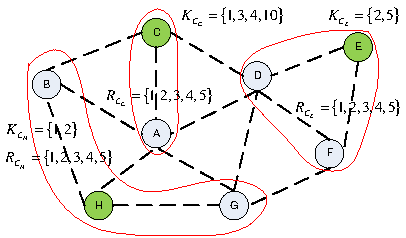
\includegraphics[width=0.5\linewidth]{figure5final.pdf}
%  \caption{Final cluster formation.}
%  \label{fig4}
%\end{figure}



This is a linear binary optimization problem, which is solved by function $bintprog$ provided in MATLAB.


Take CRN in Figure~\ref{fig1} for example.
As $|N|=8$, we let the cluster size $\delta$ to be either 2 or 3 so that the partition of network is possible.
A collection of clusters $G$ is built, where the clusters satisfy the conditions for cluster in Section~\ref{sec:model} and the sizes of clusters are 1, 2 and 3. 
$G=\{\{A\}, \{B\},\dots,\{B,C\},\{B,A\},\{B,H\},\cdots,\{B,A,C\},\{B,H,C\}, \{A,D,C\}$\\$,\cdots\}$, and $G=38$.
%Here we don't exhaustively list all the legitimate clusters with size 2 and 3.

The clustering result of binary linear programming is $\{\{D,E,F\},\{A,C,G\},\{H,G\}\}$, the number of common channels is $\{2,3,3\}$.
The solution from ROSS is $\newline \{\{B,H,G\},\{C,A\},\{D,E,F\}\}$, the number of common channels is $\{2,4,2\}$.
By applying SOC, the clustering result is $\{A,B,C,D,G\},\{E,F\},\{H\}$.

The final clusterings of the example CRN by SOC and linear programming are as follows,

\begin{figure}[ht]
\begin{center}
%\subfigure[ROSS]{\label{fig:final_clustering_ross}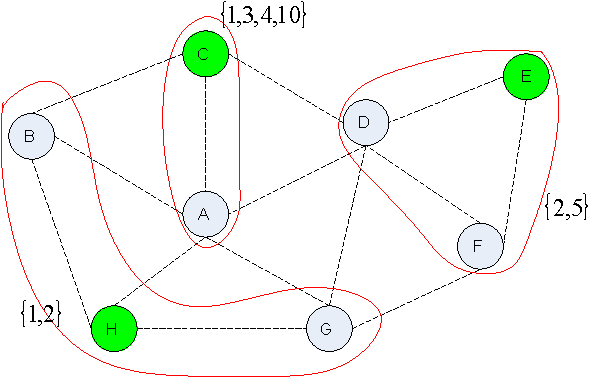
\includegraphics[width=0.3\textwidth]{final_clustering_ross}}
%
\subfigure[SOC]{\label{fig:final_clustering_soc}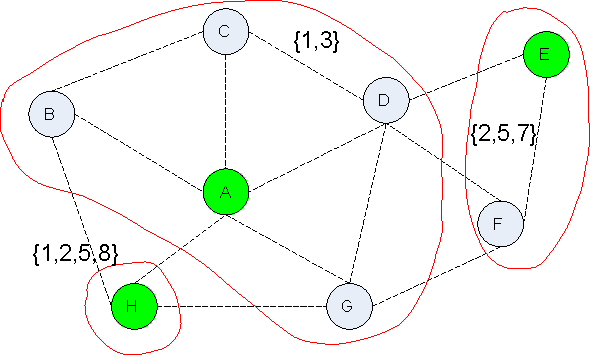
\includegraphics[width=0.45\textwidth]{final_clustering_soc}}
\subfigure[Linear programming]{\label{fig:final_clustering_LP}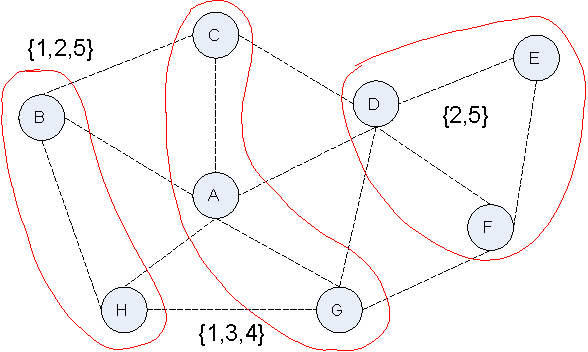
\includegraphics[width=0.45\textwidth]{final_clustering_LP}}
\end{center}
\caption{Final clustering of the example CRN}
\label{fig:final_clustering}
\end{figure}

As to the average number of common channel, the results of ROSS, LP and SOC are 2.66, 2.66, and 3 respectively. 
Note there is one singleton cluster $C_H$ generated.
When the singleton cluster $\{E\}$ is excluded, the average number of common channels of SOC drops to 2.5. 




\section{Performance Evaluation}
\label{performance}
In this section, we evaluate the performances of the two variants of ROSS, \ie ROSS-DGA and ROSS-DFA, besides, the cluster size control scheme is also evaluated when the desired cluster size is smaller than the average neighbourhood size.
We choose SOC as comparison scheme.
To the best of our knowledge, SOC~\cite{Lazos09} is the only work emphasizing on the robustness of clustering structure from all previous work on clustering in CRN. The authors of~\cite{Lazos09} compared SOC with other schemes based on the average number of common channels within each cluster, on which SOC outperforms other schemes by 50\%-100\%. This is because the schemes except for SOC are designed either for ad hoc network without consideration of channel availability~\cite{Basagni99}, or for CRN  but just considering basic connection among CR nodes~\cite{Zhao07}. Hence, we only compare the two versions of our scheme ROSS-DGA and ROSS-DFA with SOC to show the merits of ROSS, and also compare with the centralized scheme to see the gap with the global optima. 
We will investigate the following metrics:
\begin{itemize}
\item Average number of common channels per un-singleton cluster. 
\begin{itemize}
\item SOC adopts the average number of common channel over all clusters, \ie including the singleton clusters. As we try to look into the robustness of clusters of CRs, we exclude those singleton clusters.
\end{itemize}  

\item Number of unclustered CRs with moderate and vigorous intensity of PRs'activities.
\begin{itemize}
\item This is the straight forward metric on robustness of clusters.
We investigate how many clusters survives when we increase the intensity of PRs' activity.
\end{itemize}

\item Cluster sizes 
\begin{itemize}
\item Specific clusters size is pursued in many applications due to energy preservation and the system design ~\cite{clustering_globecom11}.
We will present the distribution of CRs residing in the formed clusters, and the number of generated clusters through multiple simulations.
\end{itemize}

\item Number of clusters	
\begin{itemize}
\item Homogeneous clusters size is pursued.
\end{itemize}

\item Amount of control messages involved.
\end{itemize}

The simulation is conducted with C++. 
Certain number of CR and PR nodes are deployed within a squire whose edge is 100 m.
We adopt the round disk model [xxxx] to simulate transmission.
Transmission ranges of CR and PR node are 10 and 30 respectively.
As to CRs, the CR node residing within another CR node's transmission range is seen as neighbour of that CR node.
If CR node locating within one PR node's transmission range, the CR node is not allowed to use the channel which is being used by that PR.
The number of licensed channels in simulation is 10, each PR is operating on each channel with probability of 50\%.

There are two parts of simulation, in the first part, we investigate the gap between the distributed schemes with the centralized scheme.
As there is no polynomial time solution available to solve the centralized problem, we adopt a small network to compare the performances of the ROSS, SOC and the centralized solution.
In the second part, we increase the network scale and change network density to thoroughly compare the two distributed schemes.
\subsection{Centralized Schemes vs. Decentralized Schemes}
Coinciding with the system model in Section~\ref{sec:model}, 10 primary users and 20 CR users are dropped randomly (with uniform distribution) within some area of size $A^{2}$, where we set the transmission ranges of primary and CR users to $A/3$. There are $P=10$ available channels. 
With this setting, the average number of neighbours of one CR user is around 5.
Each primary user randomly occupies one channel, and CR users are assumed to be able to sense the existence of primary users and identify available channels.
When clustering scheme is executed, around 7 channels are available on each CR node.
All primary and CR users are assumed to be static during the process of clustering.
Performance results are averaged over 50 randomly generated topologies with equal parameters.
The desired cluster size is 3.
The confidence interval shown in figure corresponds to 95\% confidence level.

\subsubsection*{Number of Common Channels}
\label{ccc_20}
We first have a look at the average number of common channels per cluster, which is used in~\cite{LIU_TMC11_2} as the sole criterion for clustering robustness.
Figure~\ref{ccc_per_nonsingleton} shows the average number of common channel of non-singleton clusters, as the singleton clusters (in other words unclustered nodes) don't execute any functionalities of clusters, which are described in Section~\ref{intro}.
As to schemes, centralized schemes outperform distributed schemes on number of common channels.
SOC achieves the most number of CCC than variants of ROSS.
SOC is liable to group the neighbouring CRs which share the most abundant spectrum together, no matter how many of them are, thus the number of CCC of the formed clusters is higher, but this method leaves considerable number of CRs which have less spectrum not in any clusters.
As to variants of ROSS, the procedure of debatable nodes greedily looking for better affiliation improves the number of CCC, thus ROSS-DGA with and without size control outperform ROSS-DFA and its size control version respectively.
We also notice that, the size control feature doesn't affect the number of CCC for both ROSS-DGA and ROSS-DFA.


\begin{figure}[ht!]
  \centering
  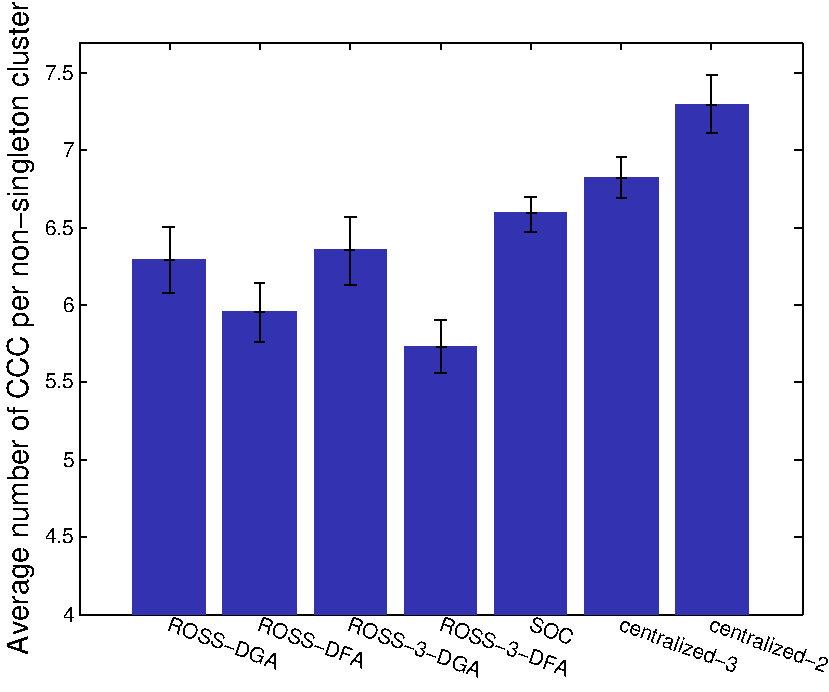
\includegraphics[width=0.65\linewidth]{ccc_20.pdf}
  \caption{Number of common channels for non-singleton clusters, the numbers in the names of schemes annotate the desired cluster size.}
  \label{ccc_per_nonsingleton}
\end{figure}

\subsubsection*{Survival Rate of Clusters with Increasing PR Users}
We investigate the robustness of the formed clusters when they co-exist with varying intensity of PRs' activities.
After the clusters are formed under the influence of the initial 10 PRs, extra 100 PRs are sequentially added into the network.
The transmission range and channel occupancy of the new PR is the same with the previous ones, \ie transmission range is $A/3$, and one channel out of 10 is randomly chosen to operate.
As to one cluster, if there is no common channels available for all members because of the new added PRs, the cluster destroyed, and the former cluster member CRs become unclustered CRs.

Figure~\ref{singleton_clusters} shows the number of unclustered CRs with the increase of PRs, which indicates the vulnerability of clusters under varying surrounding of licensed spectrum.


We obtain three conclusions corresponding to three comparisons shown in this figure,
\begin{itemize}
\item Centralized scheme with cluster size of 2 produces the most robust clusters, and SOC results in the most vulnerable clusters.
Centralized scheme with cluster size of 3 achieves less unclustered CRs than variants of ROSS when the number of PRs is 10$\sim$30, when number of PUs is 30$\sim$60, same amount of unclustered CRs are generated with variants of ROSS.
When there are 75 and more new PRs, centralized scheme with cluster size of 3 results in more unclustered CR nodes than variants of ROSS.
Size control feature makes both ROSS-DGA and ROSS-DFA outperform themselves without size control when number of new PRs is greater than 50.

The reason that centralized scheme with cluster size of 3 does not completely excel variants of ROSS is due to the favourable achievement of it: the uniformly sized clusters.
As distributed schemes, variants of ROSS generate considerable amount of smaller clusters which are more likely to survive when PRs' activities become intense.
The comparison on cluster sizes will be given in details in~\ref{cluster_size}.

\item ROSS with size control is better than the other two distributed schemes.
The size control decreases the clusters size and makes the clusters more robust when under PRs' activity.

\item Greedy algorithm improves survival rate. 
ROSS-DGA improves the survival rate of ROSS-DFA, so does ROSS-DGA with size control against ROSS-DFA with size control.
This comply with the observation on number of CCC in section~\ref{ccc_20}.
As the debatable CRs greedily update their affiliation with demanding clusters, and the metric for updating is the maximum increase of CCCs of the demanding clusters, the average number of common channels is improved (shown in Figure~\ref{ccc_per_nonsingleton}), then the robustness of clusters is enhanced. 
Meanwhile, sizes of more clusters become smaller also contributes more robustness.

\end{itemize}

\begin{figure}[ht!]
  \centering
  \includegraphics[width=0.7\linewidth]{survival_rate_20.pdf}
  \caption{Number of CRs which are not included in any clusters}
  \label{singleton_clusters}
\end{figure}

%\begin{figure}[ht!]
%  \centering
%  \includegraphics[width=0.5\linewidth]{singleton_clusters.pdf}
%  \caption{Comparison between Rocsi and centralized scheme on non-singleton clusters}
%  \label{singleton_clusters2}
%\end{figure}


\subsubsection*{Cluster Size Control}
\label{cluster_size}
\begin{figure}[ht!]
  \centering
  \includegraphics[width=0.8\linewidth]{cdf_clusterSize_20.pdf}
  \caption{Distribution of CRs residing in clusters with different sizes, as to ROSS with size control feature, the desired cluster size is 3. The average number of neighbours is 4.838.}
  \label{size_control}
\end{figure}
Figure~\ref{size_control} shows the number of CRs residing in certain sized clusters.
The centralized schemes are able to form clusters which strictly satisfy the requirement on cluster sizes.
When the desired size is 2, each generated cluster has two members.
When the desired size is 3, in average only 3 CRs are formed into 2 node clusters.
When ROSS-3-DFA is applied, most number of CRs are in 3 node clusters, nevertheless, slightly less nodes are found in 2 node and 4 node clusters, there are also considerable number of singleton clusters.
ROSS-3-DGA decreases the clusters sizes and results in more 2 node clusters, the second most CRs are found in 3 node clusters.
ROSS-DGA and ROSS-DFA generate rather even distribution of nodes with different sizes, whereas SOC results in more CRs unclustered or clusters of large sizes. 
Figure~\ref{size_control} shows distributed clustering schemes are not able to control cluster sizes perfectly, but ROSS-DGA and ROSS-DFA eliminate the clusters whose size diverges largely with the desired one, \ie single node clusters and clusters with size of 13 and 14.
Particularly, size control enable both ROSS-DGA and ROSS-DFA to achieve clusters whose sizes demonstrate certain homogeneity, \ie cluster sizes vary from 1 to 4.
But there are considerable number of single node clusters, which is due to the cluster pruning discussed in section~\ref{cluster_pruning}.

\subsubsection*{Control Signalling Overhead}
%Different from the clustering schemes proposed in ~\cite{LIU_TMC11_2, clustering_globecom11}, 
As to any variants of ROSS, there are two phases, in the first phase, clusters are formed, in the second phase, cluster membership is decided so that each node only resides in one cluster.
Control message exchanges between CR nodes are involved in both phases.

In this section we compare the amount of control messages involved for clustering in different schemes, \eg centralized scheme, ROC, ROSS-DGA, ROSS-DFA and those with size control feature.
In order to highlight the amount of control signalling only for clustering, we omit the control messages used for neighbourhood discovery, which are regarded the same for all schemes, and only compare the number of control messages brought in by the features of the schemes. 
The control message here refers both broadcast and unicast.

As to variants of ROSS, in the first phase, after each node broadcasts their new knowledge on spectrum robustness, cluster is automatically formed by cluster head which is decided from consensus by comparing the spectrum robustness with neighbours, then the cluster head broadcasts message containing its ID and the available channels in its cluster.
As to ROSS with size control feature, there are same amount of cluster heads with ROSS without enabling size control feature, and the cluster head broadcasts the available channels of the pruned cluster.
Afterwards in the second phase, membership clarification of debatable nodes is conducted.
Debatable node informs the cluster which it going to stay and the cluster head broadcasts message about its new cluster.
As to SOC, each node needs to maintain one cluster, the final clusters are formed after three rounds of comparisons and cluster mergers, while as to ROSS, only debatable nodes need to communicate with cluster heads to clarify their membership.
%1. update membership to form X1, 
%2. broadcast new X1, form new X2
%3. broadcast X3

Worst case protocol complexities.
We assume that the protocols execute synchronously. 
We compare the Time Complexity (TC), defined as the number of steps required to perform a protocol operation, and the Communication Complexity (CC), defined as the number of broadcast in performing the operation.

The complexity parameters are the number of nodes $n$ in network, number of clusters $h$.

The quantitative analysis of amount of control overhead and the size of messages are illustrated in Table \ref{tab_overhead}, 

\begin{table}[hc]
\center
\begin{tabular}{|p{3 cm}|p{3 cm}|p{7.5 cm}|}
\hline
 Scheme 		&   Number of broadcast  	& Content of message \\ \hline
 ROSS-DGA, ROSS-x-DGA 		&   $h+2*m^2c$  (upper bound)				& $ID_{H_C}$ and $V_C$ for $h+m^2c$ times, notification to join in one cluster for $m^2c$ times					\\ \hline
 ROSS-DFA, ROSS-x-DFA 		&   $h+ 2m$	 (upper bound)				& $ID_{H_C}$ and $V_C$ for $h+m$ times, notification to join in one cluster for $m$ times	 					\\ \hline
 SOC 			&   $3*n$					& $\{V_i\}, i\in M\subseteq Nb_i$						\\ \hline
 Centralized	&	$n$						& $\{C\}$         	\\ \hline
\end{tabular}
\caption{Singalling overhead. Notations: $n$-number of CR nodes in CRN, $h$-number of cluster heads, $m$-number of debatable nodes, $c$-number of demanding clusters, $\delta$-desired cluster size}
\label{tab_overhead}
\end{table}


\begin{figure}[ht!]
  \centering
  \includegraphics[width=0.67\linewidth]{number_controlMsg.pdf}
  \caption{Number of control messages}
  \label{control_msg}
\end{figure}


\subsection{Comparison between Distributed Schemes}
In this part we investigate the performances of distributed schemes in CRN with different network scales and densities.
The transmission range for CR is $A/10$ whereas $A/5$ for PR.
The number of PR is 30, we investigate the CRN where number of CR is 100, 200 and 300, and the average number of neighbours of each CR is 9.5, 20, and 31.


\subsubsection*{Number of CCC per Non-singleton Clusters}

\begin{figure}[ht!]
  \centering
  \includegraphics[width=1\linewidth]{ccc_large_scale_color.pdf}
  \caption{Number of common channels for non-singleton clusters. As to ROSS with size control feature, we adopt $x=6$ when $N=100$, $x=12$ when $N=200$, $x=21$ when $N=300$, which is around $2/3$ of the number of average neighbours}
  \label{ccc_large_scale}
\end{figure}
Figure~\ref{ccc_large_scale} shows the 
Figure~\ref{ccc_large_scale} illustrates the average number of CCC of the non-singleton clusters.
It shows when $N=100$, variants of ROSS have 30\% less CCC than SOC, but this gap is decreased when $N$ is 200 and 300.
This means SOC performs better on average number of CCC per non-singleton clusters when network density is small, which is already observed in section \ref{ccc_20}.
When the network becomes more dense, ROSS-DGA achieves even more CCC than SOC, and ROSS-DFA and ROSS-x-DGA visibly increase their performances on CCC.



\subsubsection*{Survival Rate of Clusters with Increasing PR Users}
With the increase of PRs in the network, clusters become broken as no CCC available within the clusters.
In this part of simulation, we add 290 more PRs randomly in CRN with interval of 10 to evaluate the robustness of clusters.
Figure~\ref{singleton_clusters_100} shows the increasing tread of the number of singleton clusters with the increase of PRs.
SOC generates around 10 more singleton clusters than the variants of ROSS, which accounts for 10\% of the whole network.
The confidence intervals of the variants of ROSS are not shown in the figure as they overlap, and we only show the average values.
It can be seen that greedy algorithms result in slightly less singleton clusters than their counterparts.

Figure ~\ref{singleton_clusters_300} shows a more dense CRN where $N=300$.
SOC noticeably causes more singleton clusters than ROSS variants, except for ROSS-3-DFA when PRs are few.
The reason is ROSS-3-DFA only conduct cluster membership once, which leaves large number of singleton clusters, while, in ROSS-3-DGA increase the size of smaller clusters through debatable nodes' repeated updates.

\begin{figure}[h!]
  \centering
  \includegraphics[width=0.7\linewidth]{survival_rate_100.pdf}
  \caption{Number of CRs which are not included in any clusters, $N=100$}
  \label{singleton_clusters_100}
\end{figure}

\begin{figure}[h!]
  \centering
   \includegraphics[width=0.7\linewidth]{survival_rate_300.pdf}
  \caption{Number of CRs which are not included in any clusters, $N=300$}
  \label{singleton_clusters_300}
\end{figure}

From the Figure~\ref{singleton_clusters_100} and \ref{singleton_clusters_300}, we can see greedy versions of ROSS is more robust than their counterpart variant of ROSS.
When the network is more dense, the improvement on cluster sizes and robustness by the greedy search is more obvious.


\subsubsection*{Cluster Size Control}

The number of formed clusters is shown as Fig.~\ref{nClusters_largeNetwork}.

\begin{figure}[h!]
  \centering
   \includegraphics[width=0.7\linewidth]{nClusters_largeNetwork.pdf}
  \caption{Number of formed clusters}
  \label{nClusters_largeNetwork}
\end{figure}
When the network becomes denser, more clusters are generated by SOC compared with ROSS variants.
To know the generated clusters better, we depict the cluster sizes with with cumulative distribution.

Cluster size analysis is made when the number of PRs is 30.


\begin{figure}[h!]
  \centering
   \includegraphics[width=0.7\linewidth]{cdf_clusterSize_100.pdf}
  \caption{100 CRs, 30 PRs, the average number of neighbours is 9.5.}
  \label{cdf_clusterSize_100}
\end{figure}

\begin{figure}[h!]
  \centering
   \includegraphics[width=0.7\linewidth]{cdf_clusterSize_200.pdf}
  \caption{200 CRs, 30 PRs, the average number of neighbours is 20}
  \label{cdf_clusterSize_200}
\end{figure}


\begin{figure}[h!]
  \centering
   \includegraphics[width=0.7\linewidth]{cdf_clusterSize_300.pdf}
  \caption{300 CRs, 30 PRs, the average number of neighbours is 30}
  \label{cdf_clusterSize_300}
\end{figure}

%\begin{figure}[ht]
%\begin{center}
%%\centering
%\subfigure[100 CRs, 30 PRs]{\label{result1:1}\includegraphics[width=0.48\linewidth]{cdf_clusterSize_100.pdf}}
%\subfigure[300 CRns, 30 PRns]{\label{result1:2}\includegraphics[width=0.48\linewidth]{cdf_clusterSize_300.pdf}}
%\end{center} 
%\caption[Cluster sizes]{Distribution of CRs in clusters with different sizes} %{\subref{a}, \subref{b}, \subref{c}, \subref{d}}
%\label{result1}
%\end{figure}

We see in Figure~\ref{result1:1}, when variants of ROSS are applied, most CRs are included into clusters with size of 2, thereinto, ROSS-2-DGA achieves the some homogeneous result, \ie, there is no cluster whose size is greater than 3, and the number of CRs in 2 node cluster is greater than that resulted from ROSS-2-DFA.
This is due to in the phase that debatable nodes clarify their membership, greedy search not only increases the number of CCC of relevant clusters, but also lets debatable nodes stay in smaller cluster, as shown in algorithm~\ref{alg4}.
SOC doesn't have size control feature thus the cluster sizes diverge greatly.
In a more dense network with 300 CRs, where desired size is 3, 94\% of CRs are integrated into 2 or 3 node clusters by ROSS-3-DGA, as to ROSS-3-DFA, 13\% CRs constitute singleton clusters, and 27\% CRs are within 4 node clusters.
Cluster size spans over a large range for schemes which don't have cluster size control mechanism.
As to ROSS-DGA, ROSS-DFA and SOC, 95\% of CRs stay in clusters whose sizes are smaller than 8, 9 and 14 respectively.



\begin{comment}
In the first case, there are 100 CR nodes while primary users are increased from 10 to 150. More primary users lead to fewer idle channels available in the whole network, and thus cause a challenge to the formation of clusters. In Figure~\ref{result1:1}, the average number of inner common channels achieved by the three approaches decreases with increasing the number of primary users. ROSS-DGA/DFA outperform SOC by at most $15\%$ in this case.
In Figure~\ref{result1:2}, we present the average number of outward common channels. Here, ROSS-DFA outperforms SOC by $20\%$-$40\%$ due to putting CR nodes with bigger connectivity degree at the border of clusters to strengthen the connection among them. % while the advantage of ROSS increases the more primary users are active. 
ROSS-DGA performs slightly better than ROSS-DFA on the whole range due to its larger number of iterations.

For the second scenario, we vary the number of CR nodes from 100 to 500 while keeping the number of primary users fixed at 100. Hence, we investigate the behavior of the three schemes in sparse and dense situations. Figure~\ref{result2:1} shows the average number of ICCs. We observe that ROSS-DGA/DFA achieves more ICC in sparse networks while slightly less in dense networks. We attribute this to two reasons, firstly, SOC pursues the maximal product of cluster size and number of ICC, so the product value is assured in many cases by decreasing cluster size to get more ICCs. Actually, there is a large number of clusters with only one member. %Figure \ref{result3:2} shows that the number of such clusters delivered by SOC is 120\% more than that of ROSS. 
Secondly, ROSS-DGA/DFA builds clusters on the basis of one-hop neighborhood, and dense network means there are more CR nodes within the neighborhood, thus agree on less ICCs. Figure~\ref{result2:2} demonstrates an increasing advantage of ROSS-DGA/DFA against SOC on number of outward common channels, because more nodes with bigger connectivity degree are put as border nodes. The distribution of cluster sizes are presented in Figure~\ref{result3:1} and \ref{result3:2} with variation of density. We observe that clusters formed by ROSS-DGA/DFA have similar size. Note in particular that the number of one-node clusters generated by SOC is much bigger than that produced by ROSS-DGA/DFA in both cases. This becomes especially a problem as the density increases. 

Compared with ROSS-DGA, we can find from the simulation that ROSS-DFA has much less complexity by scarifying a little performance, and both ROSS-DGA and ROSS-DFA are less complex that SOC which has a complexity of the order of $\vert I\vert^4$. This was confirmed by the run times of the simulations, which were significantly longer when simulating SOC.

\begin{figure}[t]
\begin{center}

%\centering
\subfigure[100 PRns, varying CRns]{\label{result2:1}\includegraphics[width=0.45\linewidth]{CR_ICC_3curves.pdf}}
\subfigure[100 PRns, varying CRns]{\label{result2:2}\includegraphics[width=0.45\linewidth]{CR_OCC_3curves.pdf}}
 \end{center}
\caption[]{Connectivity robustness of ICCs and OCCs with varying density of CR nodes.} %\subref{node A in $C_C$}, \subref{node A in $C_H$}}
\label{result2}
\end{figure}

\begin{figure}[ht!]
\begin{center}
%\centering
\subfigure[100 CRns, 100 PRns]{\label{result3:1}\includegraphics[width=0.45\linewidth]{distribution_1_matlab.pdf}}
\subfigure[200 CRns, 100 PRns]{\label{result3:2}\includegraphics[width=0.45\linewidth]{distribution_2_matlab.pdf}}
 \end{center}
\caption[]{Distribution of cluster sizes for two fixed scenarios.} %\subref{node A in $C_C$}, \subref{node A in $C_H$}}
\label{result3}
\end{figure}	

\end{comment}


\section{Conclusions and Future Work}
\label{conclusion}
We investigate extensively the robust clustering problem in CRN, which is important to form clusters which maintains unbroken to the greatest extent possible under primary users' activity.
We prove the NP hardness of the problem and one distributed and light weighted clustering scheme ROSS-DGA is proposed.
The clusters resulted from ROSS-DGA and its faster version ROSS-DFA are less vulnerable compared with other distributed clustering schemes, and demonstrates similar survival rate with centralized scheme under primary users' influence.
An light weighted cluster size control mechanism is contained in both ROSS-DGA and ROSS-DFA, which is advantageous for cooperative sensing and network operation with clusters.
Furthermore, considerable less control messages are generated when compared with other clustering schemes.

The drawback of this scheme is it does not form big clusters, which is attributed to that ROSS forms cluster based on cluster head's neighbourhood, and does not absorb CR nodes outside of the neighbourhood.
Big clusters could be demanded when the network density is low.

%Our work is in process, in which a light weighted clustering scheme is proposed. Intra connectivity is ensured by the border nodes, which has larger number of common channels with its neighbors within its vicinity, inter connectivity is guaranteed by deleting certain one-hop away nodes out of clusters to increase the set of common channels by a game theory approach. In this way, bigger value of  $\bar{N_{inter}}\times\bar{N_{intra}}$ could be achieved. 

%There are several issues can be investigated on the basis of current work of spectrum sharing. Firstly, as our scheme adapts multi-radio communication, channel assignment within and between clusters can be implemented to decrease interferences caused by co-channel interferences, this topic is pretty new in the scenario of cognitive radio. Secondly, the second phase of our clustering scheme can be optimized by letting nodes locating in more than one cluster use coalitional strategies, although the complexity could be higher. Thirdly, the number of the neighboring nodes is not considered when deciding cluster heads, which need to be examined in the future.

\chapter{SPECTRUM AWARE VIRTUAL COORDINATE ASSIGNMENT AND ROUTING IN MULTIHOP COGNITIVE RADIO NETWORK}
%\section{Introduction}
%\label{introduction}
%
%refer this one!! %[routing_CRN_challenges_solutions_2011]
%
%We propose Spectrum Aware Virtual Coordinate (SAViC) for multi hop cognitive radio network (CRN) to facilitate geographic routing.
%The proposed virtual coordinates (VC) of any two secondary users reflect both geographic distance and opportunistic spectrum availability between them. As a result, geographic routing is able to detour the area affected by licensed users or cut through the area with more available spectrum.
%According to different spectrum occupation patterns of primary user, two versions of SAViC are designed based on the channel utility and primary user's sojourning time respectively.
%Simulation shows the proposed virtual coordinate facilitates geographic routing to achieve high success rate of path construction.
%When duty cycle on the licensed channel is heterogeneous in the network, channel utility based virtual coordinate supports geographic routing to outperform a state-of-the-art geographic routing protocol by 40\% on packet delivery ratio. 
%When the channel utility is identical on each secondary node, and the sojourning time of primary users for secondary users are different from each other, SAViC based on primary user's sojourning time achieves significantly shorter delay than other virtual coordinates.


%en route"  on or along the way when you are going to a place

\section{Introduction}
\label{introduction}
Cognitive radio technology is promising to solve the significant shortage of spectrum, which is due to proliferation of wireless devices.
According to the definition of FCC (Federal Communications Commission in U.S.), cognitive radio is a device which is able to sense, measure, or learn its environment and accordingly tune its radio operating parameters (like center frequency, bandwidth and transmit power) on the fly, i.e. during operation. 
In this chapter cognitive radio equipment is also called secondary user.
Together with these features secondary users are allowed to reuse licensed spectrum which is authorized to so called licensed users.
%\footnote{Terms licensed and primary, user and node, as well as spectrum band and channel are used indistinguishably in the following paper.}
The cognitive radio devices are capable of vacating a spectrum band if the licensed users reappears in order not to cause harmful interference to them.

Since primary users' activity demonstrates different patterns~\cite{commag-Khalife08}, the availability of licensed spectrum exhibits different dynamics accordingly.
In certain scenarios the licensed spectrum occupancy stays available for fairly long time, \eg TV white space~\cite{SenseLess2011}.
In that case the licensed spectrum occupancy can be seen as static during a long period of time.
In other scenarios primary users' states change frequently, but measurements~\cite{Wellens200910, measurement_Palaios14} show that the percentage of time that licensed spectrum is occupied at a specific location or during a certain period of time doesn’t change, i.e. in city down town during the work time, the duty cycle of spectrum occupancy by cellular network is stable.

To fully exploit the potential of the secondary spectrum, it is crucial to investigate routing in dynamic spectrum environment.
The dynamic availability of spectrum causes frequent break down of links between secondary users, and leads to prevalent topology changes, which makes spectrum aware routing difficult but essential~\cite{routing_CRN_challenges_solutions_2011}.
%Additionally, nodes at different locations have different view on available spectrum bands.
%Measurement shows although the availability of licensed spectrum changes drastically in short time span, it demonstrates constancy at a specific location during a certain period of time~\cite{Wellens200910}, i.e. the usage of licensed spectrum in cellular network in city down town is table during the work time.
%Routing schemes are proposed in~\cite{Abbagnale_Gymkhana10, caodv-10wd, segment-crowncom08} for CRN where primary users change their operating parameters infrequently.
%More challenging scenarios with highly dynamic primary users are discussed in~\cite{Routing-crn-INFOCOM11}, where the statistics of primary users' activity is utilized in routing decision.
%A class of packet forwarding strategies for dynamic spectrum CRN is proposed in~\cite{routing-crn-icc11, routing-crn-jsac12}.
%Whenever a secondary user needs to forward a packet, it chooses channel and hop jointly based on channel's statistical characteristics observed beforehand.
%Forwarding decision is made for each single packet, which requires complex computations, large amount of control overhead, and customized media access control mechanisms.

Recent measurement in~\cite{measurement_Palaios14} shows the spectrum occupancy doesn't have significant spatial correlations between different locations.
It follows that licensed spectrum is used by primary users heavily in some areas, whereas in the other areas licensed spectrum is available over longer timespan for secondary users to use.
It is obvious to see that a routing path is better to go through the areas where primary users occupation is lower, as this alleviates or avoids the burden to cope with the changing or totally occupied spectrum when forwarding packets potentially with latency requirements.
Geographic routing is a natural choice to realize this geography sensitive routing path.
Geographic routing is light weight regarding the determination of next hop, and achieves high scalability in various wireless networks~\cite{geoRouing-qos-2009}. %
Merely knowing the geographic locations of its neighbours and the destination, a node is able to locally choose the next hop which has the smallest distance to the destination.
%As a result, control messages for route discovery are not necessary, and since the routing state maintained per node is independent on the network size, geographic routing scales perfectly.
However, in CRN dynamic link state renders geographic routing unsuccessful since packets are forwarded to the destination along the shortest path rather than avoiding areas heavily influenced by primary users.
%Coordinates indicate not only the physical distance among SUs, but also the transmission opportunities in between could leverage the strengths of geographic routing even in CRNs.

To enable geographic routing in CRN, in this chapter we propose SAViC, spectrum aware virtual coordinates for secondary users in multi-channel multi-hop CRN.
The virtual coordinate is independent of real geographic position, and has been proposed to represent the properties of the media like, link quality~\cite{Alizai_11_probabilisticAddressing} or hop numbers~\cite{gpsfree05infocom}.
Following this line of thought, our proposed virtual coordinate represents the spectrum occupancy of primary users. 
On top of this, we propose the geographic routing scheme which decides the next hop with Euclidean distance metric, and detours the areas affected by primary users, or cuts through the area with lower spectrum occupancy.
With SAViC, geographic routing imposes little computation on deciding the next hop, and requires less communication cost transmitting packet to next hop.
%it doesn't need real geographic location.
%The contribution of this paper is a novel spectrum aware virtual coordinate system for CRN.
%Secondary user firstly gets simple statistics of primary user's operation in its vicinity by spectrum sensing, then receives its virtual coordinate based on its neighbour's virtual coordinate and the channel availability at its location after light weighted arithmetic computation.
%Routing in multi-hop CRN is split up into two relatively simpler problems. 
%Firstly geographic routing decides on the next hop with virtual coordinate, then opportunistic spectrum access is conducted on the link to the chosen node.
As to our knowledge, this is the first work integrating the spectrum usage by primary users into network coordinates in order to support geographic routing in CRN, which carries meanings especially for those resource restricted devices which want to work with licensed frequency band.
The remainder of the chapter is organized as follows, after reviewing related work in Section II, system model is introduced in Section III.
Assignment of SAViC is explained in Section IV, followed by opportunistic access during transmission in Section V.
Section VI gives performance evaluation, concluding remarks are given in the last section.


\section{RELATED WORK}
When secondary users are static and primary users' operation activity is known, i.e., primary users occupy a certain channel for long time, or they occupy a channel with fixed probability, then centralized routing schemes for CRN can be designed\cite{centralized_routing_07dyspan}.
%Cellular network working with TV white space falls into this category.
%A centralized scheme is designed to build end to end path which has the optimal spectrum access opportunity in~\cite{Abbagnale_Gymkhana10}, where the availability of spectrum is regarded as static and with clear 0/1 state.
%\cite{centralized_routing_07dyspan} treats routing in CRN as a combinatorial optimization problem with consideration of link disruption probabilities.
But as centralized scheme requires sensing result from each secondary user in the network, thus suffers from any change of channel state of secondary users~\cite{Abbagnale_Gymkhana10}, besides, one centralized controller is needed to calculate the routing path on the basis of collected information from the network~\cite{centralized_routing_07dyspan, Routing-crn-INFOCOM11}.
Considerable amount of distributed schemes are proposed to cope with routing in CRN where spectrum state is usually considered to be rapid changing.
\cite{caodv-10wd} proposes CAODV (Cognitive Ad-hoc On-demand Distance Vector) and let each CR node explore all channels and store route for each available channel.
CAODV requires frequent message exchange between secondary users to maintain the up to date connections on each channel due to PU's activities, which is a burden for secondary user when primary users' activity is intense. 
\cite{segment-crowncom08} improving the DSR scheme (Dynamic Source Routing) by letting RREQ messages record spectrum availability, link quality and congestion possibility along routing paths, but it also suffers from frequently changing channel state.
%originated from DSR and AODV are proposed in~\cite{segment-crowncom08} and~\cite{caodv-10wd} respectively.
%Authors of~\cite{Routing-crn-INFOCOM11} see routing problem from the perspective of network operator. They model the vacancy of licensed spectrum with random numbers, and formulate a optimization problem to minimize the amount of needed licensed spectrum, meanwhile relevant constraints are followed for frequency selection and routing.

To cope with the rapid change of channel state, some routing schemes abandon routing table and let the transmitter decide the next hop for each single packet based on spectrum state between transmitter and neighbours.
%The sender opportunistically decides the channel availability and next hop for every single packet.
When there is packet to send, secondary user evaluates channel availability based on the statistics of sensing history~\cite{routing-crn-icc11}, or the prediction on channel availability in the forthcoming time slot~\cite{routing-crn-jsac12}, then secondary user chooses the favoured channel and next hop node to send out the packet.
Distance to the destination is also a consideration for choosing next hop.
Such per-packet forwarding paradigm reacts swiftly on the fast changing channel state, but it requires more powerful computation power on secondary users.
Firstly, that scheme produces high computation complexity on determining the channel and next hop node, secondly, specifically designed MAC mechanism and large amount of control messages are needed to coordinate the communication between the sender and the potential next hop nodes, these aspects make it uneconomic for many networks, e.g, wireless sensor networks operating with licensed spectrum~\cite{delay-cogwsn-2014}.
Furthermore, as this kind of routing paradigm emphasizes on finding the maximal transmission opportunity of secondary spectrum, the selection on preferred channel decreases the scope of next hop neighbours, thus it may yield route which does not reach the destination~\cite{commag-Khalife08, spectrumDecision_2013mass}.

%Geographic routing based routing schemes are also proposed to suit the dynamic spectrum in CRN network. 

Chowdhury et al.~\cite{search_geo_routing_chowdhury} proposes \textit{SEARCH} which is a valuable attempt to avoid the primary users' influences on routing path on the basis of geographic routing. 
%which exploits secondary channels in multiple channel CRN.
In \textit{SEARCH}, the source node launches geographic routing on each channel, and every routing path bypasses the nodes where corresponding channel is unavailable.
Paths on different channels will merge on the nodes where path circumvent happens, if such change of path and switch of channel lead to shorter time needed to send packets to destination.
After receiving the routing message on each channel, the destination decides the shortest path and sends back notifications along the chosen path.
The routing path is blocked when one primary user locating along it changes its state from OFF to ON, thus source node needs to periodically launch route request to update the routing path which may have been invalid.
\textit{SEARCH} adopts routing table and doesn't involve frequent overhead exchanges.

xxxxx


We propose a routing paradigm in CRN.
Geographic routing is applied in the CRN network which is assigned with spectrum aware virtual coordinates.
The dynamic availability of spectrum leads to prevalent topology changes, which makes spectrum aware routing difficult but essential.
Routing schemes are proposed in~\cite{Abbagnale_Gymkhana10, caodv-10wd, segment-crowncom08} for CRN where primary users change their operating parameters infrequently.
Highly dynamic primary users impose great challenge on routing, as is discussed in~\cite{Routing-crn-INFOCOM11}, where the statistics of primary users' activity is utilized in routing decision.
A class of packet forwarding strategies for dynamic spectrum CRN is proposed in~\cite{routing-crn-icc11, routing-crn-jsac12}.
Whenever a secondary user needs to forward a packet, it chooses channel and hop jointly based on channel's statistical characteristics observed beforehand.
Forwarding decision is made for each single packet, which requires complex computations, large amount of control overhead, and customized media access control mechanisms.
The solution provided by Chowdhury et al.\cite{search_geo_routing_chowdhury} improves geographic routing in multiple channel CRN by introducing circumventing mechanism, \ie when the next hop chosen based on geographic routing metric (\eg Euclidean distance) is affected by primary user, the routing packet chooses a neighbour of that node free from primary user's affection so as to avoid the primary user affected area.
Such routing is conducted on all channels, afterwards a path merge process is undertaken and one path with alternating channel is finally formed with consideration of end to end delay.

As the decision of the next hop is largely decided by the channel availability on the time point of decision, the node chosen as next hop may not be able to work after a short while due to primary user's reappearance.
Thus, this scheme works well when the primary user's activity is infrequent, but when it goes tense, the frequent invalidity of nodes due to lack of available spectrum seriously deteriorates routing performance.


xxxxxxx


\section{SYSTEM MODEL}

We consider a CRN composed with secondary users which are randomly and statically deployed in a plane.
There are orthogonal licensed channels denoted by set $C$, and secondary user is allowed to use any of them if no primary user is detected on that channel by the secondary user.
One common control channel (CCC) in license-exempt band is available for all secondary users to exchange control messages.
Only one licensed channel is used for payload transmission.
Primary users are static, and they occupancy spectrum in a constant manner, \eg the percentage of time that they access a certain channel is static in any period of time.

%Each secondary user is equipped with two half-duplex cognitive radios, one is used for control signalling exchange on CCC, the other one is used for payload transmission on licensed channel.

Proactive spectrum sensing is conducted locally and periodically as Figure~\ref{fig:sensing_period} shows. % in collaborative manner periodically~\cite{spectrum-discovery-tmc08}.
\begin{figure}[ht]
\centering
\includegraphics[scale=1]{sensing_period.pdf}
\caption{Sensing duration $T_s$ and sensing period $T_p$}
\label{fig:sensing_period}
\end{figure}



The sensing duration $T_s$ includes both detection time in physical layer and the decision synchronisation time.
Sensing period $T_p$ is the time between two successive sensing durations.
If the channel is sensed as busy\footnote{Concrete sensing techniques are not discussed in this chapter.} in sensing duration, which means at least one primary user in the vicinity is in ON state, we say the state of primary user is labelled as ON in the following sensing period $T_p$.
If not a single primary user is sensed, primary users in vicinity in the following sensing period is said to be in state OFF.
Secondary user senses each licensed channel for time $T_{access}$ with round robin scheduling, and records statistics of ON/OFF states of that channel at its place.
%In the process of transmission, as sensing is still conducted every $T_s+T_p$ time, the sensing record is updated by the sensing result in the previous $T_{access}$ time. 
%Spectrum sensing is conducted periodically, the statics on ON/OFF states are stored to update the virtual coordinate when needed.
%Such statistics are used to give quantitative spectrum availability on each node, which is further used to obtain spectrum aware virtual coordinate, besides, they are also adopted as reference to choose working channel when sending packets.


\section{Spectrum Aware Virtual Coordinates}
In this section, we firstly introduce how spectrum aware virtual coordinate is assigned, then we introduce two normalized spectrum utilities on secondary user adopted in the virtual coordinate assignment process.
One of them is called \textit{normalized spectrum availability} which is on the basis of duty cycle of primary users' absence, the other is called \textit{normalized longest blocking time} which as the name tells, is based on the lengths of time durations that primary users are detected.

Virtual coordinate has been proposed in sensor and ad hoc networks~\cite{gpsfree05infocom,Alizai_11_probabilisticAddressing}.
%Virtual coordinate is able to replace actual physical position for geographic routing in many different scenarios.
In the left part of Figure \ref{fig:vc_intro}, nodes are labelled with physical positions.
The right hand side part shows the same network assigned triplet virtual coordinate for each node according to VCap~\cite{gpsfree05infocom}, where each element of the coordinate denotes the minimal number of hops away from corresponding anchor.
This kind of virtual ordinate belongs to tree based virtual coordinates, and is obtained based on anchors which locate at the edge of network.
Anchor messages are broadcast from anchors, each of them contains a counter recording the number of hops travelled.
The minimum counter of the arriving anchor messages constitutes the corresponding element of the virtual coordinate on the arrival node.
Except for the hope numbers away from certain anchor node, virtual coordinate can also be composed with link quality~\cite{Alizai_11_probabilisticAddressing} in wireless sensor networks.
The hop based virtual coordinate is independent on actual physical position, but %reflects distance and closeness of nodes on certain aspects, and can 
supports greedy geographic routing successfully \cite{gpsfree05infocom, Alizai_11_probabilisticAddressing}.
%xxxxx The euclidean distance calculated with virtual coordinate is adopted in geographic routing.
For example, when the source-destination is B and D, and Euclidean distance calculated with virtual coordinate is adopted in the routing decision, then the greedy geographic routing achieves the same routing path in both networks: $B\rightarrow C\rightarrow D$. This path is one with the shortest traversal distance.


\begin{figure}
\centering
\includegraphics[scale=0.5]{vc_intro.pdf}
\caption{Left: nodes with physical locations, Right: nodes with doublet virtual coordinate, each element in the virtual coordinate is the number of hops away from corresponding anchor. Connecting lines denote the communication is possible.}
\label{fig:vc_intro}
\end{figure}


In this chapter, we propose licensed spectrum aware virtual coordinate in CRN, which enables geographic routing to find the path with better available spectrum.
%First of all we briefly introduce the virtual coordinates assignment protocol (VCap)~\cite{gpsfree05infocom} which is designed for wireless sensor networks working with unlicensed spectrum band.
Figure~\ref{fig:SA-VCapidea} shows one CRN where secondary users are assigned virtual coordinate according to anchor 1.
The transmission opportunity of the nodes locating within primary users' transmission range, \eg node A and C, is decreased due to sporadic spectrum, as a result, the cost for packet transmission, \eg transmission delay and energy consumption, is increased.
We integrate this obstacle caused by spectrum scarcity to transmission into virtual coordinate.
%When the anchor message arrives at node D, the counter add itself with a quantified value representing the spectrum availability, and the new value of the counter becomes the virtual coordinate of the arrival node.
%For example, as node A and C are influenced by primary users, the quantified spectrum availability on them is 3 and 4, on the other hand, quantified spectrum on node B, E, D is 1. 
%When we apply the anchor spreading as defined by VCap, and replace hop with quantified spectrum availability, we obtain the virtual coordinate for each node as Figure~\ref{fig:SA-VCapidea} shows.
%The definition of quantified spectrum is introduced in section~\ref{CA_VC_likelihood} and \ref{BT}.


%Obviously, how to characterize the channel availability (or equivalently, PU's influences) with link length is critical for the design of spectrum aware VC.
\begin{figure}
\centering
\includegraphics[scale=0.5]{CAVCap_idea_paper.pdf}
\caption{A network under primary users' influence assigned with SAViC, only anchor 1 is adopted. Flooding of anchor messages is not shown.}
\label{fig:SA-VCapidea}
\end{figure}


\subsection{Assign Spectrum Aware Virtual Coordinate}

%Similar with VCap~\cite{gpsfree05infocom}, SAViC consists of four rounds of anchor message flooding initiated from four anchors $A$, $X$, $Y$, $Z$ respectively.
As to SAViC, anchors broadcast anchor messages which flood over the network and result in virtual coordinate for each secondary user.
Several anchors are needed to assign unique virtual coordinate for each secondary user.
How to select anchors is out of the scope of this chapter.
%Each round of anchor message flooding results in one value on each node, and the last three values $x$, $y$, $z$ compose the triplet of virtual coordinate $\{x,y,z\}$.
%Besides, each node also has one auxiliary quadruplet virtual coordinate $\{a',x',y',z'\}$ which is used to decide on anchors.
In the following, we introduce how is virtual coordinate decided on each node with respect to anchors.
%Each coordinate is composed with four elements which correspond to four anchors $A$, $X$, $Y$, $Z$ respectively.


Each secondary user maintains its virtual coordinate which is one $r$-tuple where each element contained corresponds to one anchor, and the tuple length is $r$.
The elements of virtual coordinate on each node is set as big positive value.
An anchor message is generated on the anchor, which contains a $counter$ whose value is set as 0.
The anchor message is broadcast on control channel.
The influence of primary users on a secondary user is quantified as spectrum utility $\lambda$ on that secondary user.
The bigger value indicates heavier spectrum occupation by primary users.
$\lambda$ will be discussed in Section~\ref{CA_VC_likelihood} and \ref{BT}.

When a node $i$ receives an anchor message from the $t$th anchor, $i$ compares the $t$th element in its current virtual coordinate with the sum of the $\lambda$ and $counter1$ which is contained in the arriving anchor message.
%When a secondary user receives anchor message originating from anchor $A$, it adds the normalized channel availability $\Psi$ (introduced in next subsection) on itself and VC\_counter which is contained in the message, and compares the summation with its own $VC_i$.
If the sum is greater than the $t$th element in its current virtual coordinate, which indicates that the path traversed by this anchor message exposes to more active primary users, node $i$ drops the anchor message.
If the sum is smaller than the $t$th element in its current virtual coordinate, the node set the $t$th element as the sum and updates $counter1$ contained in the anchor message before forwarding it.
%The acquisition of auxiliary coordinate \textit{a'} is very similar with that for virtual coordinate.
This process is presented as Algorithm~\ref{algo:receiveAnchorMessage}.
% which also applies to obtain virtual coordinate and auxiliary coordinate in other rounds.
The process ceases within a period of time.
\begin{lemma}
\label{savic:lemma1}
As to one anchor, the number of times for each node to forward anchor message is bounded by $g$, where $g$ is the number of one hop neighbours of anchor.
\end{lemma}

\begin{lemma}
\label{savic:lemma2}
The counter value of one anchor message is increased when it is forwarded.
\end{lemma}
\begin{proof}
This is proved by the lines 18-20 in Algorithm~\ref{algo:receiveAnchorMessage}.
\end{proof}

\begin{lemma}
\label{savic:lemma3}
One anchor message affiliated with one anchor accesses the one secondary user at most twice.
\end{lemma}
\begin{proof}
Assume one node is accessed by the same anchor message for two times.
When the anchor message arrives at the secondary user, let's say $i$, for the first time, there is $\text{vc} > counter+\lambda$, and both of the vc and counter in the anchor message are updated to be $counter+\lambda$.
After being forwarded, the anchor message travels at least one other secondary user before arriving $i$, and the counter is greater than the counter value when it is forwarded from $i$ according to Lemma \ref{savic:lemma2}, which means, current counter value is greater than $\lambda_i$, and the anchor message is dropped.
Thus, this anchor message accesses secondary user $i$ for at most two times.
\end{proof}

\begin{theorem}
\label{savic:theorem_anchorMsg}
The number of anchor message corresponding to one anchor is bound by $2*g*n$, where $n$ is the number of secondary users.
\end{theorem}
\begin{proof}
This is proved by Lemma~\ref{savic:lemma1} and \ref{savic:lemma3}.
\end{proof}

According to Theorem~\ref{savic:theorem_anchorMsg}, every secondary users obtains virtual coordinate which respects to all anchors after a finite time duration.
%The algorithm for secondary user $i$ to receive one element $vc_i$ is given in Algorithm~\ref{algo:receiveAnchorMessage}.
\begin{algorithm}[!h]
\caption{Secondary user $i$ obtains one element $vc_i$ in its VC with respect to an anchor}%, $\lambda_i$ is normalized spectrum availability on $i$}          % give the algorithm a caption
\label{algo:receiveAnchorMessage} 
\DontPrintSemicolon
\SetAlgoLined
\KwIn{$vc_i =M$, $M$ is one big positive number}
%\KwOut{}
\lnl{InRes1}\If {$i$ is anchor}{
\lnl{InRes2}$vc_i=0$;\\
%\lnl{InRes3}$VC\_counter=\Psi_i$ \\ %\tcc*[f]{or $\Lambda_i$, based on }
\lnl{InRes4} set $counter1=\lambda_i$ in anchor message;\\
\lnl{InRes5} broadcast anchor message;\\
}

\lnl{InRes6}\If{receive anchor message}{
\lnl{InRes7}\eIf{$counter +\lambda_i \geqslant vc_i$}{
\lnl{InRes8}drop anchor message;}{
%\lnl{InRes9}$VC\_counter + \Psi_i < VC_i$  \\
\lnl{InRes9}$vc_i=counter + \lambda_i$;\\
\lnl{InRes10}set $counter=vc_i$ in anchor message;\\
\lnl{InRes11}broadcast anchor message;
}
}
\end{algorithm}


% which previously was stable at a low level during a long period of time. 



%and the two resultant virtual coordinates, duty cycle based virtual coordinate and blocking time based virtual coordinate.
%They are used to construct virtual coordinates which are tailored for different applications, i.e. file transmission which requires higher PDR, or instant communication which demands small end to end delay.
%virtual coordinate Dissemination


\subsection{Normalized Spectrum Availability on Secondary User}\label{CA_VC_likelihood}
Based on the statistics of primary user's ON/OFF states in time duration $T_{assement}$ which contains multiple $T_s$, secondary user $i$ characterizes the likelihood that one licensed channel, say $k$, is available at its own position with \textit{duty cycle}, which is
\begin{equation}
\label{gamma}
\gamma_i^k = \frac{\Delta_{\textsc{\tiny OFF}}}{\Delta_{\textsc{\tiny OFF}}+\Delta_{\textsc{\tiny ON}}},
\end{equation}

%\begin{equation}
%\label{likelihood_channel}
%\begin{aligned}
%\gamma_i^k = \frac{\Delta_{\textsc{\tiny OFF}}}{\Delta_{\textsc{\tiny OFF}}+\Delta_{\textsc{\tiny ON}}}
%\end{aligned}
%\end{equation}
where $\Delta_{\textsc{\tiny OFF}}$ is the number of sensing periods when channel $k$ is sensed as OFF in $T_{assement}$.
%$\gamma_i^k$ represents the likelihood that $i$ is allowed to access the licensed channel $k$.
To implement SAViC whose resultant Euclidean distance between two nodes reflects both influence from primary users and distance in terms of hops, we need to design a normalized quantified spectrum availability $\lambda_i$.

\subsubsection*{Single licensed channel}
When there is only one licensed channel in CRN (the superscript of channel $\lambda$ is omitted), the normalized spectrum availability on node $i$ is proposed as,% (upper script for channel is omitted for clarity), 
\begin{equation}
\lambda_i = -\ln \gamma_i+ c \cdot \gamma_i
\label{singCH_onehop_dc_metric}
\end{equation}

%As $\gamma_i$ denotes the possibility that one CR can deal with on packet at one time, for the path composed with series of CR nodes, the possibility that the packet travels through the path without going to buffer due to primary users occupying channel is the product of $\gamma_i$ on all nodes along the path.
%The virtual coordinate obtained by Algorithm~\ref{algo:receiveAnchorMessage} and equation~\ref{singCH_onehop_dc_metric} and 
With Formula \ref{singCH_onehop_dc_metric}, when one anchor message which originates from anchor $X$ is forwarded from node $a$ to $b$ without being dropped, the distance based on virtual coordinate reflects both the spectrum availability and geographic distance in terms of hops between the two nodes.
Based on Algorithm~\ref{algo:receiveAnchorMessage} and Formula~\ref{singCH_onehop_dc_metric}, the distance in dimension X is, 
\begin{equation}\label{distance}
\begin{split}
|x_b-x_a| & =  \sum_{i\in P_{(a,b]}} (-\ln\gamma_i + c\cdot \gamma_i) \\
		  & = -\ln(\prod_{i\in P_{(a,b]}} \gamma_i) + c\cdot \sum_{i\in P_{(a,b]}} \gamma_i
\end{split}
\end{equation}
here $x_a$ and $x_b$ are virtual coordinates of node $a$ and $b$ in dimension X respectively.
$P_{(a,b]}=(\cdots, b)$ denotes the list of nodes after $a$ and till $b$, which forward the same anchor message.

The reason to choose the form of Formula~\ref{singCH_onehop_dc_metric} is as follows.
As Formula~\ref{distance} shows, the first item is logarithm of the product of consecutive spectrum availability likelihood of the nodes in $P_{(a,b]}$.
The product is the likelihood that one message travels from node $a$ to $b$ without hampered by primary users, which is an important property we want to integrated into our virtual coordinate system.
The fist item will be infinity when the spectrum is occupied by primary users during all the time, where $\gamma=0$.
In this case, infinity can be replaced with a large positive value which results in a large $\lambda$.
The second item denotes number of hops, which can be seen clearly when $\gamma_i=0$ for node $i\in P_{(a,b]}$.

As $\lambda_i$ needs to be monotonically decreasing with respect to $\gamma_i$, so that the less spectrum availability results in bigger cost for communication, thus there should be
\begin{equation}
\frac{\partial\lambda_i}{\partial\gamma_i} = c -\frac{1}{\gamma_i} <0
\label{singCH_dc_metric_decreasing}
\end{equation} 
hence the tuning parameter $c$ should be smaller than 1.
In the simulation part, we choose $c=0.2$ so that $\lambda$ visibly reflects the changes of $\gamma$ when $\gamma$ is not too small, as Figure~\ref{fig:gamma_lambda} shows.

\begin{figure}
\centering
\includegraphics[scale=0.7]{gamma_lambda.pdf}
\caption{Normalized spectrum availability with respect to the likelihood of spectrum being available one a node}
\label{fig:gamma_lambda}
\end{figure}

%identical virtual coordinate not to be given when nodes locate out of primary user's transmission range.
%In that case the second item is positive (the first item becomes 0), so node receives a distinguishing virtual coordinate from the neighbour where the anchor message is sent out.
%and we can tune the coefficient c to adjust the weight of hops.

%2. If $a$ and $b$ don't have any coordinate obtained from the same anchor message, the distance between the two nodes with virtual coordinate is limited times of the real distance.
%see figure!!!

%Echoing the idea of virtual coordinate assignment in Figure \ref{fig:SA-VCapidea}, this function should be monotonically decreasing with respect to $\lambda_i$, thus the tuning parameter $c$ should be smaller than 1.ZA


\subsubsection*{Multiple licensed channels}
When multiple licensed channels are allowed to use without interfering primary users, one node can switch to an another channel which is at present available to send or forward packet, then the normalized channel availability is,
\begin{equation}
\gamma_i = 1-\prod_{k=1}^{|C|} (1-\gamma_i^k)
\label{gamma_multichannel}
\end{equation} 
Based on Formula~\ref{singCH_onehop_dc_metric}, the normalized spectrum availability on node $i$ when multiple secondary channels are available is,
\begin{equation}
\label{mulCH_onehop_dc_metric}
\begin{aligned}
\lambda_i & = -\ln \gamma_i+ c \cdot \gamma_i\\
		&= -\ln(1-\prod_{k=1}^{|C|}(1-\gamma_i^k)) + c \cdot (1-\prod_{k=1}^{|C|}(1-\gamma_i^k))
\end{aligned}
\end{equation}


\subsection{Normalized Longest Blocking Time on Secondary Users}
\label{BT}
Channel utility introduced in previous subsection characterizes the likelihood that secondary user is allowed to forward packets, but it fails to reflect the availability of spectrum in a finer granularity of time.
For instance, in the period of time $T_{access}$ to access the spectrum availability, one channel which frequently changes between state ON and OFF due to primary users' violent operation may have the same likelihood of available spectrum with the channel where primary user sojourns on state ON for long time.
This difference has direct consequence on delay when the likelihood of spectrum availability on PU affected secondary nodes is homogeneous.
%As to the two circumstances, when one secondary user has packet to send but spectrum is occupied completely by primary users at that time, this node needs to wait different length of time before the spectrum becomes available again, which is fundamental to end to end delay.

Let ${T_{ON}^k}$ be the length of time period that channel $k$ is not available, there is ${T_{ON}^k} = n\cdot (T_s+T_p)$, where $n$ is the number of consecutive sensing duration that channel $k$ is sensed as busy.
${T_{ON}^k}$ is recorded within $T_{access}$, and we use $\tau^k = \overline {T_{ON}^k}$ to denote the average value of the time duration that channel $k$ is occupied by primary user, which is the maximum time period that secondary user is blocked from sending/forwarding.
%$\tau^k$ models when channel is not available, the average maximal time needed to wait before the spectrum opportunity comes back again.

\subsubsection*{Single licensed channel}
In single licensed channel scenario, the normalized maximum blocking time on node $i$ is (superscript $k$ is omitted), 
\begin{equation}
\label{eq:SingleChannel_blockingtime}
\begin{aligned}
\lambda_i = f(\tau_i) = \gamma_i\cdot \tau_i + b\cdot e^{-\gamma_i\cdot \tau_i}
\end{aligned}
\end{equation}

%proposed new metric:
%\begin{equation}
%\label{eq:SingleChannelEWTLM}
%\begin{aligned}
%\lambda_i = f(\tau_i) = -\ln\gamma_i\cdot \tau_i + b\cdot e^{-\gamma_i\cdot \tau_i}
%\end{aligned}
%\end{equation}

%We multiply $\tau$ with likelihood $\gamma$ in the first item to let $\lambda$ describe channel availability more completely.
The first item is the product of blocking time and the duty cycle of available spectrum, note that we assume the duty cycle is identical for any PU affected secondary user and thus can be regarded as constant.
As to the secondary users which locate out of any primary user's transmission range, there is $\tau_i=0$, then $\lambda_i=b$, $\lambda_i$ denotes hop count in this case.
This is the reason that the second item is needed.

Same with the analysis in section~\ref{CA_VC_likelihood}, when one anchor message travels through path $P_{(a,b]}$, the distance on the corresponding coordinate dimension is the sum of the normalized longest blocking time, which is the function of the sum of maximum blocking time on the cascaded nodes on the trajectory of anchor message,

\begin{equation}
\label{distance2}
\begin{split}
|x_b-x_a| & =  \sum_{i\in P_{(a,b]}} (\gamma_i\cdot \tau_i + b\cdot e^{-\gamma_i\cdot \tau_i}) \\
		  & = \gamma_i\cdot \sum_{i\in P_{(a,b]}}\tau_i + b\cdot e^{-\gamma_i\cdot \sum_{i\in P_{(a,b]}}\tau_i}
\end{split}
\end{equation}

%As to get virtual coordinate, secondary user simply adds its normalized maximum delay onto the $counter$, so that its virtual coordinate denotes the maximum delay on the trajectory from it to anchor.

Normalized longest blocking time $\lambda$ is monotonically increasing with $\tau_i$, which requires
\begin{equation}
\begin{split}
\frac{\partial\lambda_i}{\partial\tau_i}=\gamma_i-\gamma_i\cdot b\cdot e^{-\tau_i\cdot \gamma_i}  >0\\
b  < e^{\gamma_i\cdot \tau_i}
\end{split}
\end{equation}
then we set the tuning parameter $b$ as 1.

\subsubsection*{Multiple licensed channels}
In multiple licensed channel scenario, $\tau_i$ equals to the smallest maximum blocking time over all secondary channels on node $i$, 
\begin{equation}
\tau_i = \min \tau_i^x, x\in C
\end{equation}
The normalized maximum blocking time on node $i$ is as Formula~\ref{eq:SingleChannel_blockingtime} shows.

%\begin{equation}
%\label{Tau}
%\lambda_i = f(\tau_i^k) = \gamma_i^k\cdot \tau_i^k+ b\cdot e^{-\gamma_i^k\cdot \tau_i^k}, 
%\end{equation}

%and $b$ should satisfy $b < e^{\tau_i^k\cdot \gamma_i^k} $

%where $k = \underset{c}{\operatorname{argmin}} \tau^k, c\in C$.
%In a word, $\Lambda_i$ is decided by the smallest $\tau_i$ over all secondary channels.


In remainder of this chapter, the virtual coordinate based on normalized spectrum utility is referred as \textit{spectrum availability based VC}, and The virtual coordinate based on normalized maximum blocking time is denoted as \textit{blocking time based VC} out of convenience.

%\subsubsection*{Distinct virtual coordinate} 
%Except for the \textit{spectrum availability} and \textit{blocking time} based virtual coordinate introduced in this section, other metrics of spectrum opportunities in CRN~\cite{spectrumDecision_2013mass} are also possible to be integrated into virtual coordinate, while, the validity of the idea of spectrum availability based virtual coordinates is not harmed.
%Due to the expressions of channel availability from Formula~\ref{singCH_onehop_dc_metric} to~\ref{Tau}, virtual coordinate is not integer but real number, thus there is little chance for nodes in a vicinity share the same coordinate.

 

%With SAViC, the size of zones where nodes are signed with identical virtual coordinate if applied with VCap is decreased, because $\lambda$ brings in the primary users' activity and alter the virtual coordinate of nodes which otherwise locates in the zone.
%To obtain virtual coordinate according to SA-VCap, each SU needs to broadcast once in each phase as is shown 
%Large amount of control messages are involved in generating VCs, but whenever 
When $\lambda$ on secondary nodes is identical, the resultant SAViC appears to be similar with hop based virtual coordinate.
In reality, as the measurement shows in \cite{measurement_Palaios14}, heterogeneity of spectrum usage by primary users is very normal, besides, the two kinds of virtual coordinates make it easier to find out such heterogeneity.
\cite{measurement_Palaios14} also shows within certain frequency band, primary users' activity is stable for hours, \eg cellular network.
When primary user's operation pattern changes, \eg occupy spectrum with increased duty cycle, then SAViC needs to be reimplemented.

\section{Geographic Routing and Opportunistic Spectrum Access}
\label{osa}
%\subsection*{Improved Geographic Greedy Routing Used in Testing}
%After SAViC is applied in CRN, geographic routing is used and the routing metric is the remaining Euclidean distance to the destination. 
Although spectrum aware virtual coordinate is the main concern of this chapter, we also introduce the geographic routing to be used as it affects the routing result directly.
With geographic routing, packet sender/forwarder chooses the neighbour which has smaller Euclidean distance to the destination.
The distance between node $i$ and destination $d$ is $\sqrt{(x_d-x_i)^2+(y_d-y_i)^2+(z_d-z_i)^2}$, when virtual coordinate can be denoted as $\{x, y, z\}$.
A trivial improvement on greedy geographic routing is implemented in network layer to mitigate the dead end problem.
When routing protocol reaches dead end node $u$ which is closest to destination, $u$ adds its ID to the packet as taboo before forwarding the packet to $v$ which is closest to the destination in its neighborhood.
The packet will not be sent to the nodes whose IDs appear to be taboos.
%As to deciding working channel in multiple channel scenario, packet sender only needs to exchange message with next hop for once (will be explained in Section~\ref{osa}).

%As discussed in \cite{gpsfree05infocom}, when VCap is applied, there exists an area of nodes which have the same virtual coordinate.
%Zone of identical virtual coordinate also appears when applying SAViC, which is discussed in Section \ref{Duplicated_Virtual_Coordinate}.
%When the packet arrives at one node with the desired virtual coordinates but wrong ID, the arriving node broadcasts to look for the node with desired ID, if get replied, the packet will be sent to the desired node.





%  in its neighborhood, but from where the routing protocol can not progress towards to the destination, either because it has no other neighbour, or its neighbours have been labelled as dead end.
%When packet reaches a dead end, it attaches the node ID into the packet, and is sent back to the sender.
%The dead end list contained in the packet will help packet forwarder decide on the next hop.
%When one node has packet to send, it chooses the neighbour which is closet to the destination (even further than the sender) as next hop as long as it is not in the dead end list encapsulated in the packet.
% Face routing~\cite{routingMetric_greedyRouting09infocom} overcomes dead end problem completely, but it is not considered here because of its complexity.

Buffer is implemented on each node, where packets stay temporally when no unoccupied licensed spectrum is available.
Secondary user resends buffered packet every period of time, and drops it if there is still no available channel after trying for 10 times.
%$T_{buffer}$ equals to the smallest average time duration that channel is occupied by primary users, which is introduced in subsection \ref{BT}.





%It is known that geographical routing is possible to get stuck at dead end node which is more closer to the detonation than all its neighbours. Lots of solutions have been proposed~\cite{routingMetric_greedyRouting09infocom, vc-mobile-2007} to solve this problem, e.g. face routing. In this work on the basis of primitive geographic greedy scheme, we implement \textit{geoGreedy+} which involves simple workarounds to cope with dead end problem and loops on routing paths.
In multiple channel CRN, after one node deciding on the next hop via geographic routing, which channel to use needs to be answered.
This problem involves considerations from many aspects, such as minimizing channel switch cost~\cite{spectrumDecision_2013mass}, mitigating co-channel interferences~\cite{DySpAN12_Di} etc..
%Channel selection is an active research topic which involves interference mitigation~\cite{DySpAN12_Di}, power control~\cite{HoangPowerChannel2010}, scheduling~\cite{MOBICOM10_retransmission}, topology control~\cite{Li11_ROSS}, etc.
We adopt a lightweight heuristic method in this chapter. 
When there is packet to send and the next hop is decided, packet sender chooses the channel in descending sequence with channel's metric, i.e., likelihood of channel availability, or blocking time.
The sender chooses the channel with the best metric, then conducts spectrum sensing in the immediately following sensing duration to determine the channel's usability.
If the channel is sensed as free to use, sender transmits \textit{request\_channel\_x} to the next hop on the control channel, when it receives the answering message \textit{channel\_x\_available} from that node, it starts communication on channel $x$ in the following sensing period.
If the channel is sensed to be busy before or among the transmission, or it receives \textit{channel\_x\_unavailable} message from next hop node, the sender moves to the channel with the second best metric, and conduct the same procedure as described above.
%As to delay based SAViC, the channel access strategy is the same as above except the metric to choose channel becomes $\tau$, the average time duration of being blocked instead of $\gamma$.




\section{Performance Evaluation}
%We show performance of SAViC on two aspects via simulation.
In this section, we present the performance of geographic routing together with SAViC.
Both virtual coordinates based on metrics of spectrum availability and blocking time respectively are evaluated.
Prior to that, the set-up of simulation is introduced.


\subsection{Simulation Setup}
In this section, we introduce the deployment of the primary users to generate various spectrum availability in the network, then introduce the important parameters in simulation.
Different from \cite{gpsfree05infocom} where simulation is conducted without considering any activities in MAC and physical layer, simulation in this chapter deploys a wireless environment which is close to reality, \eg interferences and channel shadowing are involved.


\subsubsection*{Primary Users}
Measurements~\cite{ProbabilityAndComputing, dsa_model_markov_2006} show that the sufficiently accurate statistic model of spectrum occupancy can be given by a Markovian process.
In simulation, primary user alternates state between ON and OFF as a two-state discrete time Markov chain (2TDMC).
% the process of alternating states of primary user.
%Primary user changes its state between ON and OFF according to transition probability, i.e. probability that it changes from current state to the other, or stays in the same state.
The probability that it changes from one state to the other, or stays in the same state is called transition probability.
Transition probability further decides the stationary probability of 2DTMC, which represents the percentage of time that primary user is in state ON or OFF in a long run.
The relationship between stationary probability $\Pi=\{\pi_{\textsc{\tiny ON}}, \pi_{\textsc{\tiny OFF}}\}$ and duty cycle $\gamma$ is, 
\begin{equation}
\label{stationary_probability}
\lim\limits_{T_{assement} \to \infty }{\gamma} = \pi_{\textsc{\tiny OFF}}
\end{equation}
Transition probability also decides the continuous sojourning time of primary user on a certain state, which affects the longest blocking time sensed by secondary users.
%~\footnote{The computation is not shown here because of space.}. 
Hence, by adjusting transition probability, we can let primary user operate with desired intensity, i.e. stationary probability for being in state OFF, or continuous sojourning time of being on state ON.
We denote stationary probability of state OFF as $P_{\textsc{\tiny OFF}}$, and the maximal blocking time as $T$.
In the following, we only use $P_{\textsc{\tiny OFF}}$ and $T$ to define primary user's dynamics, and omit mentioning the transition probability.
The time unite of the DTMC for primary user to follow is 0.1s.

As spectrum availability based and longest blocking time based virtual coordinates are designed for CRN which is influence by certain primary user activity, we design two primary user distributions.
% certain  where a certain regional disparity of spectrum exists, i.e., the former is suitable where primary users appear at some places or their occupation on spectrum is heterogeneous in the network, whereas the latter is designed where spectrum availability is identical across the network, but due to different operation pattern of primary users, the blocking time in some areas are different from the rest of the network.
As a result, we design two categories of primary user settings to evaluate the routing performance assisted by the two categories of virtual coordinate respectively.
\begin{itemize}
\item As to spectrum availability based virtual coordinate, two primary users are located in the CRN which can not affect all the nodes in CRN, as shown in Figure~\ref{fig:singleChannelPioff_case_topo}.
\item For blocking time based virtual coordinate, network is evenly covered by primary users which have the same duty cycle, but some primary users have different blocking time with the others, as Figure~\ref{fig:multipleChannelPioff_case_topo} shows.
%In  all primary users have the same spectrum availability, but some of them have shorter sojourning time in state ON than the others.
\end{itemize}
When multiple channel scenario is to be investigated, existing primary users simply start to work with current and additional channels, and there is no new primary users appear.



\subsubsection*{Parameter Setting}
Simulation is conducted with INET framework provided by OMNeT++ simulator~\cite{omnetpp_paper08}, which comprises both generation of SAViC and following geographic routing. 
Secondary users are randomly distributed in a square area and 6 nodes which locate at the edge are deployed as anchors.
%The transmission power of secondary users is 0 dBm, noise is -110 dBm, the SNR threshold is 4dB, sensitivity is -90dBm, path-loss coefficient is 2, Rayleigh fading is brought in the channel model.
%As a result, to the communication range is about 10\% of the whole network.
%Licensed channel works on 2.4 GHz frequency band.
%In each network, one source node is chosen to send UDP stream to one destination node, the packet size is 512k Byte. 
%The tuning parameters $c$ and $d$ for Formulas 1 to 4 are 0.2 and 1 respectively.
%We run each simulation for 1000s, the first 95s is for secondary users to trace spectrum availability, 5s is used assign SAViC to network, the rest 900s is for routing.
%All the confidence intervals (CI) are according to 95\% confidence level.

\subsection{Success Rate of Geographic Routing on Finding Path}

We evaluate SAViC's reachability, i.e. given the virtual coordinate of destination, geographic routing forwards packet from source to the node with the desired virtual coordinate.
%We see the routing path is set up as long as any node with the same virtual coordinate is reached, and this comparison don't involve any influence from primary users when the routing is conducted.
%, and hop based virtual coordinate gains benefit because there could exist several nodes assigned identical virtual coordinate with the destination node.
%For network assigned with CA-VCs, the PUs in the network are set to state OFF when conducting geographic routing.
The comparisons are real geographic location, and hop based virtual coordinate according to VCap~\cite{gpsfree05infocom}. 
We deploy 6 anchors and then there is no duplicated virtual coordinate among the resultant virtual coordinate system.
%We configure different spectrum availability in the network to investigate the reachability of SAViC, as shown in the following table.
% so adopting different configurations of primary user in the simulation doesn't arise question of cherry picking.
%As to testing channel utility based SAViC, two primary users locate in the middle of the network as shown in Figure~\ref{fig:singleChannelPioff_case_topo}, which operates with the same $P_{\textsc{\tiny OFF}}$.
%As to delay based SAViC, primary users locate as shown in Figure~\ref{fig:multipleChannelPioff_case_topo} where each cycle center locates one primary user,.
%Two scenarios present distinctive activity patterns of primary user.
%In scenario 1, $P_{\textsc{\tiny OFF}}=0.9$ for all primary users, $T_{\textsc{\tiny ON}}$ is 27s in region 2 (the lower-left area as shown in Figure~\ref{fig:multipleChannelPioff_case_topo}), and $T_{\textsc{\tiny ON}}$ of primary user is 0.33s in region 1 (the reset area except for region 2).
%In scenario 2, $T_{\textsc{\tiny ON}}$ of primary user is 3s in region 1, other parameters of primary user is the same with scenario 1.

%\begin{figure}
%  \begin{minipage}[c]{0.65\linewidth}
%    \includegraphics[width=\linewidth]{Reachability_DC_EWT.pdf}
%  \end{minipage}\hfill
%  \begin{minipage}[r]{0.32\linewidth}
%    \caption{
%			Reachability of different virtual coordinates, virtual coordinate is acronym of virtual coordinate.
%    } \label{fig:reachability}
%  \end{minipage}
%\end{figure}
%\vspace{-1cm}

\begin{figure}[ht]
	\centering
    \includegraphics[width=0.7\linewidth]{Reachability_DC_EWT.pdf}
    \caption{Reachability of different virtual coordinates, the average number of neighbors is 6, 12, and 14} 			\label{fig:reachability}
\end{figure}
%\vspace{+1cm}

%There are two configurations of primary users,
%\begin{itemize}
%\item The first is as shown by the dashed cycles in Figure~\ref{fig:singleChannelPioff_case_topo}, two primary users locate in the middle of the network, which operates with the same $P_{\textsc{\tiny OFF}}$.
%This configuration is used to test Channel availability based SAViC later.
%\item The second is as shown by the cycles in Figure~\ref{fig:multipleChannelPioff_case_topo}, which is to construct one CRN where secondary users sense the same likelihood of spectrum availability, but the blocking time in some areas are different from the rest areas.
%$P_{\textsc{\tiny OFF}}=0.9$ for all primary users, $T_{\textsc{\tiny ON}}$ is 27s for primary users in solid cycles.
%This configuration is used to test Blocking time based SAViC.
%\end{itemize}
%%\vspace*{-\baselineskip}
%\begin{center}
%    \begin{tabular}{| p{1.85 cm} | p{6.7 cm} |}
%    \hline
%    Coordinate & Configuration of primary users  \\ \hline
%    Channel availability based SAViC & As shown by the dashed cycles in Figure~\ref{fig:singleChannelPioff_case_topo}, two primary users locate in the middle of the network, which operates with the same $P_{\textsc{\tiny OFF}}$.  \\ \hline
%    Blocking time based SAViC & As shown by the cycles in Figure~\ref{fig:multipleChannelPioff_case_topo}, $P_{\textsc{\tiny OFF}}=0.9$ for all primary users, $T_{\textsc{\tiny ON}}$ is 27s for primary users in solid cycles
%    \vspace*{-.4em}
%\begin{itemize}%[noitemsep,nolistsep]
%  \item scenario 1: $T_{\textsc{\tiny ON}}$ is 0.33s in dashed cycles
%  \item scenario 2: $T_{\textsc{\tiny ON}}$ is 3s in dashed cycles
%\end{itemize}
%\vspace*{-1.2 em}
%      \\ \hline
%    VCap & No primary users \\ \hline
%    Geo-location & No primary users \\ \hline
%    \end{tabular}
%\end{center}

In order to evaluate the effectiveness of coordinates to support geographic routing, we design different configurations of primary users.
As to duty cycle based VC, two primary users are randomly deployed in the network.
As to delay based VC, we configure 9 primary users to evenly cover the network, among of them, 4 primary users have different maximal blocking time with the rest.
Under one configuration of primary users, 1000 random CRN is generated and in each CRN one far departed pair of source and destination is chosen to test.

%For each setting of primary user, simulation is done over 100 random secondary user networks, and in each network one pair of nodes locating at opposite ends of network (which have the largest distance) is chosen as source and destination.
%We configure two scenarios to test blocking time based virtual coordinate, scenario I: $T_{\textsc{\tiny ON}}=27s$ for the primary users in solid cycle in Figure~\ref{fig:multipleChannelPioff_case_topo}, 3s for the rest, scenario II: $T_{\textsc{\tiny ON}}=27s$ in region 2, 0.33s for the rest.

%Figure \ref{fig:reachability} depicts the average success rate of path construction of the network with the same scale.
Figure \ref{fig:reachability} shows, spectrum availability based virtual coordinate supports geographic routing to achieve similar reachability with hop based virtual coordinate\footnote{The numerical result of hop based virtual coordinate coincides with the simulation result presented in \cite{gpsfree05infocom} under the same network density}, which is better than that with real geographic location.
%When $P_{\textsc{\tiny OFF}}$ is smaller, utility based virtual coordinate works worse but the gap with the aforementioned is trivial.
%Geographic routing working with real geographic location performs poorer, because dead end problem is largely alleviated by VC.
Blocking time based virtual coordinate performs a little bit worse than other coordinates.
%delay based VC's effectiveness is illustrated in Subsection~\ref{subsection:SA-VCap-EWT} where utility based virtual coordinate fails to support geographic routing as PUs' likelihood are geographically homogeneous over the network.
%The success rate of geographic routing with hop based virtual coordinate coincides with the results in work~\cite{gpsfree05infocom}.
%Note the CRN in simulation is quite sparse compared with that used in~\cite{gpsfree05infocom}
In summary, after integrating the primary user's influence, SAViC supports geographic routing to achieve comparable success rate of path construction with conventional virtual coordinate and real geographic location.



\subsection{Routing Performance}
%%%%%%%%%%%%%%%%%%%%%%%%%%%%%%%%%%%%%%%%%%%%%%
%	single channel, channel utility based VC
%%%%%%%%%%%%%%%%%%%%%%%%%%%%%%%%%%%%%%%%%%%%%%
We sequentially present the routing performance of SAViC based on spectrum availability and blocking time respectively.
In more details, spectrum availability SAViC is compared with hop based virtual coordinate VCap and \textit{SEARCH}.
%Hop based virtual coordinate is testified to support geographic routing in large scale sensor networks successfully~\cite{gpsfree05infocom}.
The reason to choose \textit{SEARCH}~\cite{search_geo_routing_chowdhury} is it is on the basis of geographic routing and utilizes routing table in the interval of updates, thus it requires less computation ability and overhead exchanges.
%When one primary user which locates on the routing path changes its state from OFF to ON, that routing path is blocked, thus source node needs to periodically launch route request to update the possibly invalid path. 
The time interval for \textit{SEARCH} to update routing tables of the nodes on routing path is 5s.
%, and its effectiveness when channel utility SAViC becomes invalid in the case that  
%For this purpose, we use end to end delay as metric in addition to packet delivery ratio performance to give more insights into the working mechanism of virtual coordinate.
%We sequentially simulate the routing performance of SAViC based on channel utility and delay respectively, 
Both single and multiple licensed channel scenarios are investigated for the three solutions.

\subsubsection*{Duty Cycle Based Virtual Coordinate} \mbox{}

%\vspace{.1cm}
%\textbf{Single secondary channel scenario}

%\textit{1. Single secondary channel scenario}
We start by looking into the performance of SAViC in single channel scenario.

%\begin{figure}
%\centering
%\includegraphics[width=0.5\linewidth]{singleChannel_DC_caseStudy.pdf}
%\caption{Routing paths with different virtual coordinate paradigms}
%\label{fig:singleChannelPioff_case_topo}
%\end{figure}

%\begin{figure}[htb!]
%  \begin{minipage}[c]{0.5\linewidth}
%    \includegraphics[width=\linewidth]{singleChannel_DC_caseStudy.pdf}
%  \end{minipage}\hfill
%  \begin{minipage}[r]{0.45\linewidth}
%    \caption{
%		Routing paths with different virtual coordinate paradigms
%    } \label{fig:singleChannelPioff_case_topo}
%  \end{minipage}
%\end{figure}


\begin{figure}[htb!]
\subfigure[Routing paths]
{\label{fig:singleChannelPioff_case_topo}
\includegraphics[width=0.455\linewidth]{singleChannel_DC_caseStudy.pdf}
}
\subfigure[PDR over 50 random CRN network, PU's location is fixed as shown in Figure~\ref{fig:singleChannelPioff_case_topo}]
{\label{fig:Averaged_single_DC}
\includegraphics[width=0.455\linewidth]{singleCh_average_pdr_3.pdf}
}
\caption{Routing paths and corresponding PDR}
\label{fig:pioff_case}
\end{figure}

\begin{figure}[htb!]
\subfigure[PDR]
{\label{fig:random_SU_PU_PDR}
\includegraphics[width=0.455\linewidth]{random_SU_PU.pdf}
}
\subfigure[Delay]
{\label{fig:random_SU_PU_delay}
\includegraphics[width=0.455\linewidth]{delay_dc_c1.pdf}
}
\caption{Packet delivery ratio with single secondary channel, over 50 randomly located CR nodes and PUs}
\label{fig:pioff_single}
\end{figure}
We start with a case study, two primary users locate at the centers of dashed cycles as shown in Figure~\ref{fig:singleChannelPioff_case_topo}.
VC based on spectrum availability and VCap (hop is its metric) are assigned to secondary users separately.
The red dashed path in Figure~\ref{fig:singleChannelPioff_case_topo} is formed by geographic routing with VCap, which cuts across the primary users' affecting area and thus suffers great packet loss.
%The routing paths supported by spectrum availability based virtual coordinate is affected by the intensity of primary users, 
The black dash and blue solid paths are formed with spectrum availability based virtual coordinate, the two paths are formed when primary user's working intensities $P_{\textsc{\tiny OFF}}$ is 0.1 and 0.9 respectively. 
%snapshot of routing paths obtained by geographic routing with utility based virtual coordinate and hop based virtual coordinate respectively.
%When PUs' $P_{\textsc{\tiny OFF}}=0.1$, routing paths with corresponding utility based virtual coordinate is presented by the green dash line.
%Blue solid line denotes the routing path when $P_{\textsc{\tiny OFF}}$ is 0.9.
%It is easy to find that, when PUs are very active ($P_{\textsc{\tiny OFF}}=0.1$), the generated routing path detours the PU affected area completely, which means when calculated with DC-based VC, the distances between the nodes inside and outside of the PU affected area become larger, thus \textit{geoGreedy+} doesn't choose the PU affected SUs.
%When $P_{\textsc{\tiny OFF}}=0.9$, obtained routing path is closer to the PU affected areas, but is still out of the PU region.
These two paths vividly illustrate that utility based virtual coordinate successfully integrates the spectrum scarcity in CRN network, and decomposes a large part of routing decision.
%Packet delivery ratio corresponding to this network is shown in Figure \ref{fig:Averaged_single_DC}.
%Subfigure \ref{fig:SingleChannelPioff_case_pdr} presents the channel utility based VCs generate paths which achieve almost 100 \% packets delivery ratio when PU's $P_{\textsc{\tiny OFF}}$ changes from 0.1 to 0.9 in this topology.
%
%Now we step further to check channel utility based VC's ability to support geographical routing in 50 random secondary networks under different PU active levels. 
%To get full picture of SAViC's performance on packet delivery ratio, we change primary user' intensity, and randomize secondary users' location.
%We compare SAViC, hop based virtual coordinate along with one CRN routing scheme \textit{SEARCH}~\cite{search_geo_routing_chowdhury}.
The paths of SEARCH is not drawn here as the routing path is possible to change after path update.
We keep the primary users in the middle of the network, for each activity intensity, 50 CRNs where secondary users are randomly located are generated.
Figure~\ref{fig:Averaged_single_DC} shows the PDR of spectrum availability based virtual coordinate is high except for a minor decline when $P_{\textsc{\tiny OFF}}$ is between 0.5 and 0.8, which is contradictory to the monotonically increasing trend of hop based virtual coordinate. This can be explained by the path snapshot in Figure \ref{fig:singleChannelPioff_case_topo}. 
When channel is sensed to be scarce (primary users access channel intensively), path generated is far away from the affected area and circumvents completely.
When primary users become less intensive, routing path moves closer to that area.
In other words, the weaker dynamics of primary users attracts path and result in packet drop.
When $P_{\textsc{\tiny OFF}}$ approaches to 1, spectrum availability based virtual coordinate becomes actual hop based virtual coordinate as the link metric in formula \ref{singCH_onehop_dc_metric} becomes zero.
%The curve of VCap monotonically increase when PUs become less active, but it suffers seriously when PUs are active.
%The detour phenomenon of paths with utility based virtual coordinate can also be observed in Figure~\ref{fig:singleCh_DC_number_of_hops}, where route length becomes shorter when PU becomes less intensive.
%The routing paths supported by this two VCs and corresponding PDR performances are identical.
%the first item of the link metric in formula \ref{singCH_onehop_dc_metric} becomes 0 and hop metric becomes one constant, thus the paths and PDR performance generated by the two virtual coordinate systems are identical.

\textit{The paradox that more licensed spectrum leads to worse PDR} can also be observed on \textit{SEARCH}, whose PDR curve declines first and increases later on.
When channel is heavily utilized by primary users, the routing request is more likely to encounter operating primary user, then a node out of the primary user affecting area is chosen as next hop, so that the path experiences less packet loss (with the price of more hops).
When primary users become less intense, routing request is more likely to traverse the affected areas, as a result, the routing path experiences packet loss due to the primary users in that area before next route update. 
%PDR gets higher with increase of $P_{\textsc{\tiny OFF}}$ only after $P_{\textsc{\tiny OFF}}$ is bigger than 0.4.
%This is the reason for the drop of PDR in the middle
%When $P_{\textsc{\tiny OFF}}$ is bigger than 0.4, PDR gets higher with $P_{\textsc{\tiny OFF}}$ increases.
%As \textit{SEARCH} is based on geographic routing and works with real geographic location. The hop counts of routing path is shorter than that of SAViC and hop based virtual coordinate, as shown in Figure~\ref{fig:singleCh_DC_number_of_hops}.
%meanwhile, with PUs become less intense, the hop counts become smaller, which coincides with Figure \ref{fig:singleChannelPioff_case_topo}.

Figure~\ref{fig:random_SU_PU_PDR} shows the PDR when both primary and secondary users' locations are random.
SAViC's performance deteriorates because the source and destination may be influenced by primary users, so that a path completely detour the primary users' area is impossible. where geographic routing has no means to detour the affected areas.
In figure~\ref{fig:random_SU_PU_delay}, SAViC and SEARCH achieve lower delay although forwarding more packets, which means SAViC is effective to facilitate geographic routing to avoid PU affecting areas.


%%%%%%%%%%%%%%%%%%%%%%%%%%%%%%%%%%%%%%%%%%%%%%
%	multiple channel, channel utility based VC
%%%%%%%%%%%%%%%%%%%%%%%%%%%%%%%%%%%%%%%%%%%%%%
%\vspace{.1cm}
%\textbf{Multiple secondary channel scenario}
%\textit{2. Multiple secondary channel scenario}

%Formula~\ref{singCH_onehop_dc_metric} to~\ref{Tau} tell that the \textit{virtual distance} is monotonically increasing with the scarcity of spectrum, as SAViC has been testified to comprise routing decisions in CRN in previous simulation, we can firmly predict that SAViC based on Formulas~\ref{mulCH_onehop_dc_metric} to~\ref{Tau} also have similar out-performances with the same primary user setting.
%In the following, we create more challenging primary setting with more primary users.

%\begin{figure}[htb!]
%\centering
%\includegraphics[width=0.5\linewidth]{MultiCH_DC_casestudy_route.pdf}
%\caption{Routing paths with different virtual coordinate paradigms}
%\label{fig:multipleChannelPioff_case_topo}
%\end{figure}

%\begin{figure}[htb!]
%  \begin{minipage}[r]{0.5\linewidth}
%    \includegraphics[width=\linewidth]{MultiCH_DC_casestudy_route.pdf}
%  \end{minipage}\hfill
%  \begin{minipage}[r]{0.45\linewidth}
%    \caption{
%		Routing paths with different virtual coordinate paradigms
%    } \label{fig:multipleChannelPioff_case_topo}
%  \end{minipage}
%\end{figure}


%\begin{figure}[htb!]
%\subfigure[One CRN]{\label{fig:multipleChannelPioff_case_topo}
%\includegraphics[width=0.455\linewidth]{MultiCH_DC_casestudy_route.pdf}
%}
%\subfigure[One CRN]{\label{fig:multipleChannelPioff_case_pdr}
%\includegraphics[width=0.455\linewidth]{MultiCH_DC_casestudy_pdr.pdf}
%}
%\label{fig:multiple_pioffCase}
%\caption{Packet delivery ratio in multiple secondary channel scenario}
%\end{figure}
Now we introduce the routing performance in multiple channel scenario, where two licensed channels available, but only one is allowed for payload transmission.


\begin{figure}[htb!]
\subfigure[PDR over 50 CRNs where SUs and PUs are randomly located]{\label{fig:MultiChannel_DC_pdr}
\includegraphics[width=0.455\linewidth]{random_SU_PU_2channel.pdf}
}
\subfigure[PDR over 50 CRNs where SUs and PUs are randomly located]{\label{fig:MultiChannel_DC_delay}
\includegraphics[width=0.455\linewidth]{delay_dc_c2.pdf}
}
\label{fig:multiple_pioffCase}
\caption{Packet delivery ratio with multiple secondary channel scenario}
\end{figure}
In this part of simulation, we follow the setting of single channel scenario, except that secondary users have at most two licensed channels.
%Network with two licensed channels is shown in Figure~\ref{fig:multipleChannelPioff_case_topo}, where primary user locates at the center of each cycle.
%Each primary user works on two licensed channels which are independent with each other.
%Figure~\ref{fig:multipleChannelPioff_case_topo} shows routing paths with different virtual coordinates and primary user's intensities, where in region 2 primary user's $P_{\textsc{\tiny OFF}}$ is 0.5.
%When $P_{\textsc{\tiny OFF}}$ is also 0.5 for primary users in region 1 and all primary users have equal workload, the path generated (blue solid path) converges to the path with hop based virtual coordinate (red dashed path).
%When $P_{\textsc{\tiny OFF}}=0.9$ for primary users in region 1, channel utility based SAViC results in black dashed path which avoids the seriously affected area.
%In this case, both paths endure tremendous packet loss as shown in Figure \ref{fig:multipleChannelPioff_case_pdr}. 
%Figure~\ref{fig:multipleChannelPioff_case_pdr} shows the packet delivery ratio of the dashed black and solid blue paths.

%Figure \ref{fig:multipleChannelPioff_case_pdr} presents the PDR of the paths generated with the two VCs.
%Most of the unsuccessfully delivered packets are dropped from buffers because of the lack of usable spectrum for too long time.
Thanks to the second channel, the packet delivery radio is increased as shown in Figure~\ref{fig:MultiChannel_DC_pdr}, and delay is decreased as depicted in Figure~\ref{fig:singleChannelPioff_case_topo}.
SAViC still outperform the other schemes especially in the aspect of PDR.
%Figure~\ref{fig:MultiChannel_DC_pdr} shows the average packet delivery ratio over 50 random topologies of secondary networks, with the same configuration of primary user as that in  Figure~\ref{fig:singleChannelPioff_case_topo}.
%Due to the second available channel and the opportunistic spectrum access paradigm, the PDR of the three schemes are improved.
%Improvement brought in by the second channel can also be observed in Figure~\ref{fig:MultiChannel_DC_delay} compared with Figure~\ref{fig:random_SU_PU}.
%Packet delivery ratio of SAViC increases with primary users become less intense, the packet loss is due to the widespread primary users.
%\textit{SEARCH} performs as bad as geographic routing with hop based virtual coordinate. The reason is the widespread primary users seriously hamper the routing requests to arrive at destination, consequentially most paths for forwarding the packets can not be constructed successfully.
%Figure~\ref{fig:MultiChannel_DC_hop} illustrates a similar trend with Figure \ref{fig:singleCh_DC_number_of_hops}, when there is less differences among PUs' intensity, the length of path becomes longer.






\subsubsection*{Longest Blocking time Based Virtual Coordinate}    \mbox{}
\label{subsection:blocking_time}
%As we have pointed out in \ref{BT}, the duty cycle of channel's availability is not adequate to describe the waiting time in buffer for a packet if there is no spectrum available, thus we test the delay based virtual coordinate when all PUs' duty cycles are identical.

%This means that when primary users' certain characteristic is observed homogeneous across network, the virtual coordinate which is designed on the basis of that characteristic is not capable to comprise routing decisions any more.
%In this case another different characteristic (delay in this case) is needed to form spectrum aware virtual coordinate.

%%%%%%%%%%%%%%%%%%%%%%%%%%%%%%%%%%%%%%%%%%%%%%
%	delay based VC
%%%%%%%%%%%%%%%%%%%%%%%%%%%%%%%%%%%%%%%%%%%%%%

%\vspace{.1cm}
%\textbf{Single secondary channel scenario}
As discussed in section~\ref{BT}, spectrum availability based virtual coordinate doesn't reflect the sparsity or abundance of spectrum well when the likelihood of spectrum availability is homogeneous in CRN.
A CRN working with single licensed channel in Figure~\ref{fig:multipleChannelPioff_case_topo} is used to show the fail of spectrum availability based virtual coordinate.
Two items are used in the following to make the analysis tidy.
\begin{center}
\begin{tabular}{cl}
\toprule
 $T_1$        & Maximal blocking time of primary users  \\
				&  					whose transmission ranges are solid cycles in Figure~\ref{fig:multipleChannelPioff_case_topo}\\
\midrule  
    $T_2$       &  Maximal blocking time of the other primary users \\
\bottomrule
\end{tabular}
\end{center}
%
\begin{figure}[ht]
	\centering
    \includegraphics[width=0.6\linewidth]{topo_single_blocking_time.pdf}
    \caption{Routing paths in one network, $T_1 = 3s$. cycles denote the transmission range of primary uers.} 			\label{fig:multipleChannelPioff_case_topo}
\end{figure}
In the network, 9 primary users evenly distributed, $P_{\textsc{\tiny OFF}}=0.5$ for each of them.
For the primary users denoted by the solid cycles, maximal blocking time $T_1 = 3s$, and $T_2 = 1s$ and $3s$ for the other primary users.
When $T_2 < T_1$, the resultant routing path is in black and dashed, which goes through area where primary users have shorter maximal blocking time.
When $T_2 = T_1$, the resultant routing path largely converges with the path with VCap.

%and the $P_{\textsc{\tiny OFF}}$ of the other primary users changes from 0.5 yo 1, the PDR of the schemes is described in Figure~\ref{fig:fail_SA}.
%Note that although packet delivery ratio of SAViC increases when primary users become less intense, the packet loss of availability based virtual coordinate is only $10\%$ when there is $P_{\textsc{\tiny OFF}}=0.5$ for all primary.
%Due to the second available channel and the opportunistic spectrum access paradigm, the PDR of the three schemes are improved.
%%\vspace{.5cm}
%\begin{figure}[htb!]
%\subfigure[One CRN]{\label{fig:multipleChannelPioff_case_pdr}
%\includegraphics[width=0.455\linewidth]{MultiCH_DC_casestudy_pdr.pdf}
%}
%\subfigure[One CRN]{\label{fig:MultiChannel_DC_pdr}
%\includegraphics[width=0.455\linewidth]{multiCh_DC_average_pdr_3.pdf}
%}
%\label{fig:multiple_pioffCase}
%\caption{Packet delivery ratio in multiple secondary channel scenario}
%\end{figure}
%\vspace{.5cm}
%\begin{figure}[ht]
%	\centering
%    \includegraphics[width=0.6\linewidth]{multiCh_DC_average_pdr_3.pdf}
%    \caption{PDR of spectrum availability based virtual coordinate when likelihood is homogeneous in CRN} 			\label{fig:fail_SA}
%\end{figure}


The ineffectiveness of spectrum availability based virtual coordinate in case of identical $P_{\textsc{\tiny OFF}}$ is observed in Figure~\ref{fig:multipleChannelPioff_case_topo}.
In this case a different characteristic, i.e., the longest blocking time, which shows the geographically diverse characteristics of spectrum can be used.
In our simulation, $P_{\textsc{\tiny OFF}}=0.9$ for all primary users, but they are diverse on sojourn time, i.e. $T_1$ of primary user is 3s, and $T_2$ is shorter.
We randomize the location of secondary users in 50 networks, and present the performance of blocking time based virtual coordinate to show its superiority on decreased end to end delay and PDR.
In this part of simulation, we don't show the result of \textit{SEARCH}, as it performs as bad as geographic routing with hop based virtual coordinate.
The reason is the widespread primary users seriously hamper the routing requests to arrive at destination, consequentially most paths for forwarding the packets can not be constructed successfully.
\begin{figure}[htb!]
\subfigure[Packet delivery ratio]{\label{fig:SingleChannelEWT_randomness_rate}\includegraphics[width=0.46\linewidth]{ewt_pdr_3_ci.pdf}
}
\subfigure[Delay]{\label{fig:SingleChannelEWT_randomness_delay}\includegraphics[width=0.46\linewidth]{delay_ewt_c1.pdf}
}
\label{fig:SingleChannelEWT}
\caption{Geographic routing in single secondary channel scenario, $P_{\textsc{\tiny OFF}}=0.9$ for all primary users, $T_1=3s$, $T_2$ varies.}
\end{figure}
%

%Because of \textit{SEARCH}'s weak performance when the whole network is influenced by primary users, (PDR is less 20\% as shown in Figure~\ref{fig:MultiChannel_DC_pdr}), we only compare the performances with delay based SAViC and hop based virtual coordinate.


Figure~\ref{fig:SingleChannelEWT_randomness_delay} shows as $T_2$ increases from 0.33s to 3s, the delay of successfully delivered packets also increases for both blocking time based virtual coordinate and VCap, but a constant gap exists in between.
Whereas, the delay of spectrum availability based virtual coordinate is random as respect to sojourn time, the reason is the routing metric in this scenario doesn't involve blocking time imposed by primary users.
%This shows blocking time based virtual coordinate enables routing path to go through primary user affecting areas where they have shorter sojourn time on operating.

%Delay based virtual coordinate manipulates nodes sharing smaller blocked time to get closer, whereas $P_{\textsc{\tiny OFF}}$ based virtual coordinate doesn't adjust the network topology meaningfully.

The packet delivery ratio shown in Figure \ref{fig:SingleChannelEWT_randomness_rate} is constant with both blocking time based virtual coordinate and VCap, because all the primary users have the same $P_{\textsc{\tiny OFF}}$ which is 0.9.
Particularly, blocking time based virtual coordinate achieves higher packet delivery ratio than the other two virtual ordinates, the reason is when the former is applied, less packets are dropped from buffer as the time of being blocked is shorter for the secondary users on the path.

%\vspace{.1cm}
%\textbf{Multiple secondary channel scenario}

%\textit{2. Multiple secondary channel scenario}





%The distinctive sojourn time of PUs in region 1 and 2 makes delay based virtual coordinate much effective to support geographic routing.
Now we have a look at the CRN with two licensed channels.
As to performance of delay, because of the second available channel, blocking time based virtual coordinate achieves very delay, in contrast, spectrum availability based virtual coordinate still demonstrates obvious randomness, as is shown in Figure \ref{fig:MultiChannelEWT_delay}. 
%Because of the second available channel, delay is primary user works on one more licensed channel and with the same pattern of the first channel.
Compare Figure \ref{fig:MultiChannelEWT_rate} and \ref{fig:SingleChannelEWT_randomness_rate}, we can see the packet delivery ratio in two channel network is obviously higher than that in single channel network, as the second channel provides extra transmission opportunities.
Blocking time based virtual coordinate achieves up to 10\% better performance than that with spectrum availability based VC, the reason is packets in buffer have greater likelihood to be sent out before getting dropped.
\begin{figure}[htb!]
\subfigure[Packet delivery ratio]{\label{fig:MultiChannelEWT_rate}\includegraphics[width=0.46\linewidth]{multiCh_EWT_rate_3.pdf}
}
\subfigure[Delay]
{\label{fig:MultiChannelEWT_delay}\includegraphics[width=0.46\linewidth]{delay_ewt_c2.pdf}
}
\label{fig:MultiChannelEWT_pdr}
\caption{Geographic routing in two secondary channel scenario, $P_{\textsc{\tiny OFF}}=0.9$ for all primary users, $T_1=3s$, $T_2$ varies.}
\end{figure}
%with each transition probability combination, we run the simulation in 10 randomly generated topologies (in each topology we measure the delay only once). The Results shown in Figure \ref{fig:SingleChannelEWT_diff_topos}, SA-VCap enabled path outperforms that from VCap in all criterions. The reason for low delivery ratio is that, PUs exist all over the network.

\subsection{Sensitivity of SAViC to Estimation Errors}
In this Section, we evaluate the performance of SAViC in the presence of erroneous estimates about the primary user activity.
In order to induce a particular amount of errors, we artificially add errors to duty cycle of primary user activity by directly modifying the implementation of 2 state markov chain. 
By doing this a real life scenario is built, where estimation errors are expected.
The simulation is conducted with the same configuration with Figure~\ref{fig:singleChannelPioff_case_topo}.
Figure~\ref{fig:errorenousEsti_DC} shows even the errors are significant, \ie DC is modified by 25\% to 100\%, the corresponding performance varies only at most 13\%.


\begin{figure}[ht]
	\centering
    \includegraphics[width=0.7\linewidth]{errorenousEsti_DC.pdf}
    \caption{In the setting of Figure~\ref{fig:singleChannelPioff_case_topo}, perofrmance of DC based virtual coordinate is not affected greatly by the erroneous estimation} 			\label{fig:errorenousEsti_DC}
\end{figure}




\section{CONCLUSION}
The proposed virtual coordinate SAViC reshapes the topology of cognitive radio network based on sensing results of spectrum availability.
As SAViC adjusts the distance between nodes based on the communication obstruction caused by primary users, the virtual coordinate comprises a part of the routing decision, so that geographic routing is able to detour the areas seriously affected by primary user.
Geographic routing with SAViC greatly simplifies the computation and communication burden on each secondary user involved in routing in CRN.
Together with SAViC, geographic routing achieves better performances than other geographic routing designed for CRN through extensive simulation.
This paradigm of routing is especially suitable for CRN network where the resource limited CR nodes can only support geographic routing.
This work emphasises on avoiding primary users' influence with geographic routing, and doesn't consider the interference issue among the secondary users, which should be addressed in the future work.
%SAViC supports high reachability.
%As SAViC comprises routing decision, light weighted geographic routing circumvents the area seriously affected by primary user, or cut through the less affected area.
%Specially, geographic routing together with available channel likelihood based virtual coordinate achieve higher PDR than one representative CRN routing scheme when PUs' activities are geographically heterogeneous in the network.
%To remedy the incompetence of channel likelihood based VC, delay sensitive virtual coordinate becomes alternative to support geographic routing and produce short delay and satisfactory PDR.
%As a result, burden of computation and communication for secondary users is largely alleviated.
%The finally found path is static, which suffers from PUs' activity passively, a dynamic path adjustment scheme could be a workaround in the future work.
%\subsection{Choice on Characteristics of spectrum availability}
%The DT2MC provides a relatively comprehensive model to investigate PUs' activities.
%With the properties derived from DT2MC, we are able to design virtual coordinates emphasizing on different network performances.
%
%When primary users' characteristics are evenly distributed in the network, correspondingly designed virtual coordinate is not more effective than that based on hop number.
\chapter{Conclusion}
Cooperation is also one paradigm which is claimed to able to improve the network performance.
It requires extra control overheads because of organization.
\chapter{Appendix}

% appendix
%\backmatter
\begin{appendices}
%\appendix
%\addcontentsline{toc}{section}{Appendix~\ref{noconvergence}: Proof of Theorem \ref{noconvergence}}
\chapter{Proof of Theorem \ref{noconvergence}}
\label{proof}

For selfish best response approach, the utility function is set as follows,
	\begin{equation}
\label{selfishutility}
		u_i=\frac{\sum_{c(i)=c(i)} f_{ji}+N_0}{P_i\cdot h_i\cdot z_i}
	\end{equation}

\begin{proof}

In order to simplify the proof, we assume $N_0=0$.
Consider one WBS $i$ executing algorithm \ref{whitecatalgo} with utility \ref{selfishutility}, and updates its channel from $c_i$ to $c_i'$, we denote $u_k', k\in \mathcal{N}$ as the utility of WBS $k$ when $i$ chooses channel $c_i'$, accordingly, the summation of utilities of all WBSs after $i$ changing to $c_i'$ is $U'=\sum_{\forall k\in \mathcal{N}, c(i)=c_i'}u_k'$.
\begin{equation}
\label{xxx}
\begin{split}	
U'
& =u_i' + \sum\limits_{j\in\mathcal{N},j\neq i}u_j'\\
& =u_i' + \sum\limits_{j\in\mathcal{N},j\neq i}(u_j+(u_j'-u_j))\\
& =u_i' + \sum\limits_{j\in\mathcal{N},j\neq i}u_j+\sum\limits_{j\in\mathcal{N},j\neq i}(u_j'-u_j)\\
& =u_i' + \sum\limits_{\tiny\substack{j\in\mathcal{N},j\neq i}}u_j + \sum\limits_{\tiny\substack{j\in\mathcal{N},\\j\neq i, \\c(j)=c_i'}}(u_j'-u_j) + \sum\limits_{\tiny\substack{j\in\mathcal{N},\\j\neq i, \\c(j)=c_i}}(u_j'-u_j)\\
&  + \sum\limits_{\tiny\substack{j\in\mathcal{N},j\neq i, \\c(j)\neq c_i', c(j)\neq c_i}}(u_j'-u_j)\\
& =u_i' + \sum\limits_{\tiny\substack{j\in\mathcal{N},j\neq i}}u_j + \sum\limits_{\tiny\substack{j\in\mathcal{N},\\j\neq i, \\c(j)=c_i'}}(\dfrac{ f_{ij}}{\tilde P_j}) - \sum\limits_{\tiny\substack{j\in\mathcal{N},\\j\neq i, \\c(j)=c_i}}(\dfrac{ f_{ij}}{\tilde P_j})\\
\end{split}
\end{equation}

where,
\begin{equation}
\label{xxxx}
\begin{split}	
u_i'
& = u_i + \varDelta u_i(c_i\rightarrow c_i')\\
& = u_i + \sum\limits_{\tiny\substack{j\in\mathcal{N},\\j\neq i, \\c(j)=c_i'}}(\dfrac{ f_{ji}}{\tilde P_i}) - \sum\limits_{\tiny\substack{j\in\mathcal{N},\\j\neq i, \\c(j)=c_i}}(\dfrac{ f_{ji}}{\tilde P_i})
\end{split}
\end{equation}

bring \ref{xxxx} into \ref{xxx}, we get,
\begin{equation}
\label{xxxxx}
\begin{split}	
U'
& =U + \sum\limits_{\tiny\substack{j\in\mathcal{N},\\j\neq i, \\c(j)=c_i'}}(\dfrac{ f_{ji}}{\tilde P_i}) - \sum\limits_{\tiny\substack{j\in\mathcal{N},\\j\neq i, \\c(j)=c_i}}(\dfrac{f_{ji}}{\tilde P_i}) \\
& + \sum\limits_{\tiny\substack{j\in\mathcal{N},\\j\neq i, \\c(j)=c_i'}}(\dfrac{ f_{ij}}{\tilde P_j}) - \sum\limits_{\tiny\substack{j\in\mathcal{N},\\j\neq i, \\c(j)=c_i}}(\dfrac{f_{ij}}{\tilde P_j})\\
%& =U + \sum\limits_{\tiny\substack{j\in\mathcal{N},\\j\neq i, \\c(j)=c_i'}}(\dfrac{P_j\cdot h_{ji}+\delta}{P_i'}) - \sum\limits_{\tiny\substack{j\in\mathcal{N},\\j\neq i, \\c(j)=c_i}}(\dfrac{P_j\cdot h_{ji}+\delta}{P_i'}) \\
%& + \sum\limits_{\tiny\substack{j\in\mathcal{N},\\j\neq i, \\c(j)=c_i'}}(\dfrac{P_i\cdot h_{ji}+\delta}{P_j'}) - \sum\limits_{\tiny\substack{j\in\mathcal{N},\\j\neq i, \\c(j)=c_i}}(\dfrac{P_i\cdot h_{ji}+\delta}{P_j'})\\
\end{split}
\end{equation}
According to algorithm \ref{whitecatalgo}, the summation of second and third items, which is the variance of $i$' utility, is negative. If we can confirm the summation of fourth of the last four items is negative, the whole utility of the network decreases with $i$' each update. For simplification, we assume that the channel is symmetric, which means, $h_{ij}=h_{ji}$, and $z$ is identical among all WBSs. Then, the problem we want to confirm is equivalent to the following: Given the in-equation with $n$, $m$ are natural numbers
\begin{equation}
\label{xxxxxx}
\begin{split}	
\sum\limits_{i=1}^{m} \alpha_i < \sum\limits_{i=1}^{n} \beta_i,
\end{split}
\end{equation}
 Prove the following in-equation is correct or not,
\begin{equation}
\label{xxxxxxx}
\begin{split}	
\sum\limits_{i=1}^{m} (\alpha_i+\dfrac{1}{\alpha_i}) < \sum\limits_{i=1}^{n} (\beta_i+\dfrac{1}{\beta_i}),
\end{split}
\end{equation}
We propose a small contradiction to prove \ref{xxxxxxx} is not true.
When $m=2,n=1$, and $\alpha_1=1, \alpha_2=0.5, \beta=2.1$, we can see that although $\sum_{i=1}^m\alpha_i=1.5 < \sum_{i=1}^n\beta_i=2.1$, there is
$\sum_{i=1}^m(\alpha_i+\frac{1}{\alpha_i})=4.5 > \sum_{i=1}^n(\beta_i+\frac{1}{\beta_i})=2.58$.
hence, with WBS's update, it is possible that $U'> U$, thus there is no monotonically convergence by utilizing \ref{selfishutility}.

\end{proof}

Notice that the last four items in \ref{xxxxx} is exactly the change of summation of utilities of all WBSs after $i$' update if WhiteCat is executed, hence the monotonic convergence of WhiteCat is proved here analytically if noise is considered to be zero. If noise is considered, we can follow the conclusion in the end of \ref{gameforproblem} that WhiteCat converges without monotonicity.





%\appendix
%\addcontentsline{toc}{section}{Appendix~\ref{QLP}: reformulation of \ref{QLP}}
\chapter{Deviation of Problem \ref{QLP}}
\label{optdeviation}
We reformulate the objective problem \ref{QLP} which is a binary non-linear programming to binary quadratic programming as follows,

	\begin{equation}	
\label{QLP2_1}
		\begin{aligned}
%		\begin{split}
		& \sum\limits^{n}_{i=1} \frac{\sum\limits_{j\in\mathcal{N}, j\neq i}P^TX_j(X_j^TX_i)h_{ji}z_{ji} + N_0}{P^TX_ih_iz_i}\\
		& =\sum\limits^{n}_{i=1}( \frac{\sum\limits_{j\in\mathcal{N}, j\neq i}\sum\limits_k (P_{jk}\cdot x_{jk}\cdot x_{ik}\cdot x_{jk}\cdot h_{ji}\cdot z_{ji}) + \sum\limits_k N_0\cdot x_{i k}}{P^TX_ih_iz_i})\\
		& =\sum\limits^{n}_{i=1}( \frac{\sum\limits_{j\in\mathcal{N}, j\neq i}\sum\limits_k (P_{jk}\cdot x_{jk}\cdot x_{ik}\cdot h_{ji}\cdot z_{ji})}{P^TX_ih_iz_i}  + \frac{\sum\limits_k N_0\cdot x_{ik}}{P^TX_ih_iz_i})\\
		& =\sum\limits^{n}_{i=1}( \sum\limits_{j\in\mathcal{N}, j\neq i}\sum\limits_k \frac{(P_{jk}\cdot x_{jk}\cdot x_{ik}\cdot h_{ji}\cdot z_{ji})}{P^TX_ih_iz_i}  + \sum\limits_k\frac{N_0\cdot x_{ik}}{P^TX_ih_iz_i})
%		\end{split}
		\end{aligned}
	\end{equation}

If we assume WBS $i$ is working on channel $m$, then there is $x_{im}=1$, then the first item in the parenthesis becomes,
	\begin{equation}
		\label{QLP2_22}
				\begin{aligned}
				 &\frac{P_{jk}\cdot x_{jk}\cdot x_{ik}\cdot h_{ji}\cdot z_{ji}}{P^TX_ih_iz_i}
				 &= \frac{P_{jk}\cdot x_{jk}\cdot x_{im}\cdot h_{ji}\cdot z_{ji}}{P_{im}\cdot x_{im} \cdot h_i\cdot z_i} \\
				 &= \frac{P_{jk}\cdot x_{jk}\cdot h_{ji}\cdot z_{ji}}{P_{im}\cdot h_i\cdot z_i}
		 	\end{aligned}
	\end{equation}
%other wise, formula \ref{QLP2_22} equals to 0.

Similarly, for the second item in the parenthesis,		

	\begin{equation}
\label{QLP2_4}
			\frac{N_0\cdot x_{ik}}{P^TX_ih_iz_i} = \frac{N_0}{P_{ik}h_iz_i}\cdot x_{ik}
	\end{equation}		
		
then, formula \ref{QLP2_1} becomes,
	\begin{equation}
\label{QLP2_5}
			\sum\limits^{n}_{i=1}( \sum\limits_{j\in\mathcal{N}, j\neq i}\sum\limits_k \frac{P_{jk}\cdot h_{ji}\cdot z_{ji}}{P_{ik}\cdot h_i\cdot z_i}\cdot  x_{jk}\cdot x_{ik}  + \sum\limits_k \frac{N_0}{P_{ik}\cdot h_i\cdot z_i}\cdot x_{ik})
		\end{equation}	

which is a binary quadratic programming problem.
\end{appendices}



%%: ----------------------- glossary ------------------------
%
%% Tie in external source file for definitions: /backmatter/07_glossary.tex
%% Glossary entries can also be defined in the main text. See 07_glossary.tex
%\newglossaryentry{mac}
{
    name=MAC,
    description={Media Control Layer}
}

\newglossaryentry{rf}
{
    name=RF,
    description={Radio Frequency}
}


\newglossaryentry{wpan}
{
    name=WPAN,
    description={Wireless personal-area network}
}

\newglossaryentry{wlan}
{
    name=WLAN,
    description={Wireless local-area network}
}

\newglossaryentry{wman}
{
    name=WMAN,
    description={Wireless metropolitan-area network}
}

\newglossaryentry{3g}
{
    name=3G,
    description={Third generation}
}


\newglossaryentry{gsm}
{
    name=GSM,
    description={Global system for mobile communications}
}
 
 
 
 \newglossaryentry{5G}
{
    name=5G,
    description={5th generation mobile networks}
}
 
 
 
 
 


\newglossaryentry{FCC}
{
    name=FCC,
    description={Federal communications commission in U.S.}
}
 
 
 \newglossaryentry{CR}
{
    name=CR,
    description={Cognitive radio}
}

 \newglossaryentry{SU}
{
    name=SU,
    description={Secondary user}
}
 
 \newglossaryentry{PR}
{
    name=PR,
    description={Primary radio}
} 
 
 \newglossaryentry{PU}
{
    name=PU,
    description={Primary user}
}

 
\newglossaryentry{CRN}
{
    name=CRN,
    description={Cognitive radio network}
}
 
 
\newglossaryentry{QoS}
{
    name=QoS,
    description={Quality of service}
}


\newglossaryentry{ISM}
{
    name=ISM band,
    description={Industrial, scientific, and medical}
}

\newglossaryentry{PDA}
{
    name=PDA,
    description={Personal digital assistant}
}


\newglossaryentry{CRAHN}
{
    name=CRAHN,
    description={Cognitive radio ad hoc network}
}


\newglossaryentry{WRAN}
{
    name=WRAN,
    description={Wireless regional area network}
}


\newglossaryentry{WBS}
{
    name=WBS,
    description={White base station}
}


\newglossaryentry{ECC}
{
    name=ECC,
    description={Electronic communications committee in Europe}
}


\newglossaryentry{CCC}
{
    name=CCC,
    description={Common control channel}
}


\newglossaryentry{DCF}
{
    name=DCF,
    description={Distributed coordination function}
}


\newglossaryentry{CW}
{
    name=CW,
    description={Contention window}
}


\newglossaryentry{NE}
{
    name=NE,
    description={Nash equilibrium}
}

\newglossaryentry{PO}
{
    name=PO,
    description={Pareto optimality}
}


\newglossaryentry{PoA}
{
    name=PoA,
    description={price of anarchy}
}


\newglossaryentry{RSSI}
{
    name=RSSI,
    description={Received signal strength index}
}


\newglossaryentry{DTV}
{
    name=DTV,
    description={digital TV}
}

\newglossaryentry{SINR}
{
    name=SINR,
    description={signal-to-noise-and-interference ratio}
}

\newglossaryentry{MAN}
{
    name=MAN,
    description={Metropolitan area networks}
}

\newglossaryentry{LP}
{
    name=LP,
    description={linear programming program}
}

\newglossaryentry{WitheCat}
{
    name=WitheCat,
    description={Distributed white space channel allocation technology}
}

\newglossaryentry{COS}
{
    name=COS,
    description={Cost of oscillation}
}

\newglossaryentry{ICC}
{
    name=ICC,
    description={inner common channels}
}

\newglossaryentry{ROSS}
{
    name=ROSS,
    description={Robust spectrum sharing}
}

\newglossaryentry{ROSS-DGA}
{
    name=ROSS-DGA,
    description={Robust spectrum Sharing-distributed greedy algorithm}
}

\newglossaryentry{ROSS-DFA}
{
    name=ROSS-DFA,
    description={Robust spectrum sharing-distributed fast algorithm}
}


\newglossaryentry{TC}
{
    name=TC,
    description={Time complexity}
}

\newglossaryentry{DSR}
{
    name=DSR,
    description={Dynamic source routing}
}

\newglossaryentry{2TDMC}
{
    name=2TDMC,
    description={two-state discrete time Markov chain}
}

\newglossaryentry{VCap}
{
    name=VCap,
    description={virtual coordinate assignment protocol}
}


\newglossaryentry{CH}
{
    name=CH,
    description={cluster head}
}
%\newglossaryentry{xxxxxxxx}
%{
%    name=xxxxxxxx,
%    description={}
%}
\newglossaryentry{UHF}
{
    name=UHF,
    description={Ultra high frequency}
}


\newglossaryentry{TVBD}
{
    name=TVBD,
    description={TV band devices}
}

\newglossaryentry{TVWS}
{
    name=TVWS,
    description={TV white space}
}

\newglossaryentry{DiCAPS}
{
    name=DiCAPS,
    description={Distributed channel allocation and power selection}
}

\newglossaryentry{whiteCat}
{
    name=WhiteCat,
    description={White space channel allocation}
}

\newglossaryentry{LTE}
{
    name=LTE,
    description={3GPP Long term Evolution}
}

\newglossaryentry{HSPA}
{
    name=HSPA,
    description={High speed packet access}
}


%\begin{multicols}{2} % \begin{multicols}{#columns}[header text][space]
%\begin{footnotesize} % scriptsize(7) < footnotesize(8) < small (9) < normal (10)
%\printnomenclature[1.5cm] % [] = distance between entry and description
%\label{nom} % target name for links to glossary
%\end{footnotesize}
%\end{multicols}





%%%%%%%%%%%%%%%%%%%%%%%%%%%%%%%%%%%%%%%%%%%%%%%%%%%%%%%%%%%%%
%% LITERATUR UND ANDERE VERZEICHNISSE
%%%%%%%%%%%%%%%%%%%%%%%%%%%%%%%%%%%%%%%%%%%%%%%%%%%%%%%%%%%%%
%% Ein kleiner Abstand zu den Kapiteln im Inhaltsverzeichnis (toc)
\ifnotdraft{
\addtocontents{toc}{\protect\vspace*{\baselineskip}}
\cleardoublepage
%% Literaturverzeichnis
\phantomsection % phantomsection wird benötigt, damit z.B. hyperref die richtige Seite verlinkt.
\addcontentsline{toc}{chapter}{Bibliography}
%\nocite{*}								%Auch nicht-zitierte BibTeX-Einträge werden angezeigt.
\bibliography{./backmatter/myrefs}
\bibliographystyle{styles/acmurl}		 			%Art der Ausgabe: plain / apalike / amsalpha / ...
}

%% Abbildungsverzeichnis
\clearpage
\addcontentsline{toc}{chapter}{List of Figures}
\listoffigures

%% Tabellenverzeichnis
\clearpage
\addcontentsline{toc}{chapter}{List of Tables}
\listoftables

%Print the glossary
\clearpage
\addcontentsline{toc}{chapter}{Glossary}                 % add Glossary to TOC
\printglossary[style=mcolindex]

%%%%%%%%%%%%%%%%%%%%%%%%%%%%%%%%%%%%%%%%%%%%%%%%%%%%%%%%%%%%%
%% ANHÄNGE
%%%%%%%%%%%%%%%%%%%%%%%%%%%%%%%%%%%%%%%%%%%%%%%%%%%%%%%%%%%%%
%\appendix
%\chapter{Appendix}

% appendix
%\backmatter
\begin{appendices}
%\appendix
%\addcontentsline{toc}{section}{Appendix~\ref{noconvergence}: Proof of Theorem \ref{noconvergence}}
\chapter{Proof of Theorem \ref{noconvergence}}
\label{proof}

For selfish best response approach, the utility function is set as follows,
	\begin{equation}
\label{selfishutility}
		u_i=\frac{\sum_{c(i)=c(i)} f_{ji}+N_0}{P_i\cdot h_i\cdot z_i}
	\end{equation}

\begin{proof}

In order to simplify the proof, we assume $N_0=0$.
Consider one WBS $i$ executing algorithm \ref{whitecatalgo} with utility \ref{selfishutility}, and updates its channel from $c_i$ to $c_i'$, we denote $u_k', k\in \mathcal{N}$ as the utility of WBS $k$ when $i$ chooses channel $c_i'$, accordingly, the summation of utilities of all WBSs after $i$ changing to $c_i'$ is $U'=\sum_{\forall k\in \mathcal{N}, c(i)=c_i'}u_k'$.
\begin{equation}
\label{xxx}
\begin{split}	
U'
& =u_i' + \sum\limits_{j\in\mathcal{N},j\neq i}u_j'\\
& =u_i' + \sum\limits_{j\in\mathcal{N},j\neq i}(u_j+(u_j'-u_j))\\
& =u_i' + \sum\limits_{j\in\mathcal{N},j\neq i}u_j+\sum\limits_{j\in\mathcal{N},j\neq i}(u_j'-u_j)\\
& =u_i' + \sum\limits_{\tiny\substack{j\in\mathcal{N},j\neq i}}u_j + \sum\limits_{\tiny\substack{j\in\mathcal{N},\\j\neq i, \\c(j)=c_i'}}(u_j'-u_j) + \sum\limits_{\tiny\substack{j\in\mathcal{N},\\j\neq i, \\c(j)=c_i}}(u_j'-u_j)\\
&  + \sum\limits_{\tiny\substack{j\in\mathcal{N},j\neq i, \\c(j)\neq c_i', c(j)\neq c_i}}(u_j'-u_j)\\
& =u_i' + \sum\limits_{\tiny\substack{j\in\mathcal{N},j\neq i}}u_j + \sum\limits_{\tiny\substack{j\in\mathcal{N},\\j\neq i, \\c(j)=c_i'}}(\dfrac{ f_{ij}}{\tilde P_j}) - \sum\limits_{\tiny\substack{j\in\mathcal{N},\\j\neq i, \\c(j)=c_i}}(\dfrac{ f_{ij}}{\tilde P_j})\\
\end{split}
\end{equation}

where,
\begin{equation}
\label{xxxx}
\begin{split}	
u_i'
& = u_i + \varDelta u_i(c_i\rightarrow c_i')\\
& = u_i + \sum\limits_{\tiny\substack{j\in\mathcal{N},\\j\neq i, \\c(j)=c_i'}}(\dfrac{ f_{ji}}{\tilde P_i}) - \sum\limits_{\tiny\substack{j\in\mathcal{N},\\j\neq i, \\c(j)=c_i}}(\dfrac{ f_{ji}}{\tilde P_i})
\end{split}
\end{equation}

bring \ref{xxxx} into \ref{xxx}, we get,
\begin{equation}
\label{xxxxx}
\begin{split}	
U'
& =U + \sum\limits_{\tiny\substack{j\in\mathcal{N},\\j\neq i, \\c(j)=c_i'}}(\dfrac{ f_{ji}}{\tilde P_i}) - \sum\limits_{\tiny\substack{j\in\mathcal{N},\\j\neq i, \\c(j)=c_i}}(\dfrac{f_{ji}}{\tilde P_i}) \\
& + \sum\limits_{\tiny\substack{j\in\mathcal{N},\\j\neq i, \\c(j)=c_i'}}(\dfrac{ f_{ij}}{\tilde P_j}) - \sum\limits_{\tiny\substack{j\in\mathcal{N},\\j\neq i, \\c(j)=c_i}}(\dfrac{f_{ij}}{\tilde P_j})\\
%& =U + \sum\limits_{\tiny\substack{j\in\mathcal{N},\\j\neq i, \\c(j)=c_i'}}(\dfrac{P_j\cdot h_{ji}+\delta}{P_i'}) - \sum\limits_{\tiny\substack{j\in\mathcal{N},\\j\neq i, \\c(j)=c_i}}(\dfrac{P_j\cdot h_{ji}+\delta}{P_i'}) \\
%& + \sum\limits_{\tiny\substack{j\in\mathcal{N},\\j\neq i, \\c(j)=c_i'}}(\dfrac{P_i\cdot h_{ji}+\delta}{P_j'}) - \sum\limits_{\tiny\substack{j\in\mathcal{N},\\j\neq i, \\c(j)=c_i}}(\dfrac{P_i\cdot h_{ji}+\delta}{P_j'})\\
\end{split}
\end{equation}
According to algorithm \ref{whitecatalgo}, the summation of second and third items, which is the variance of $i$' utility, is negative. If we can confirm the summation of fourth of the last four items is negative, the whole utility of the network decreases with $i$' each update. For simplification, we assume that the channel is symmetric, which means, $h_{ij}=h_{ji}$, and $z$ is identical among all WBSs. Then, the problem we want to confirm is equivalent to the following: Given the in-equation with $n$, $m$ are natural numbers
\begin{equation}
\label{xxxxxx}
\begin{split}	
\sum\limits_{i=1}^{m} \alpha_i < \sum\limits_{i=1}^{n} \beta_i,
\end{split}
\end{equation}
 Prove the following in-equation is correct or not,
\begin{equation}
\label{xxxxxxx}
\begin{split}	
\sum\limits_{i=1}^{m} (\alpha_i+\dfrac{1}{\alpha_i}) < \sum\limits_{i=1}^{n} (\beta_i+\dfrac{1}{\beta_i}),
\end{split}
\end{equation}
We propose a small contradiction to prove \ref{xxxxxxx} is not true.
When $m=2,n=1$, and $\alpha_1=1, \alpha_2=0.5, \beta=2.1$, we can see that although $\sum_{i=1}^m\alpha_i=1.5 < \sum_{i=1}^n\beta_i=2.1$, there is
$\sum_{i=1}^m(\alpha_i+\frac{1}{\alpha_i})=4.5 > \sum_{i=1}^n(\beta_i+\frac{1}{\beta_i})=2.58$.
hence, with WBS's update, it is possible that $U'> U$, thus there is no monotonically convergence by utilizing \ref{selfishutility}.

\end{proof}

Notice that the last four items in \ref{xxxxx} is exactly the change of summation of utilities of all WBSs after $i$' update if WhiteCat is executed, hence the monotonic convergence of WhiteCat is proved here analytically if noise is considered to be zero. If noise is considered, we can follow the conclusion in the end of \ref{gameforproblem} that WhiteCat converges without monotonicity.





%\appendix
%\addcontentsline{toc}{section}{Appendix~\ref{QLP}: reformulation of \ref{QLP}}
\chapter{Deviation of Problem \ref{QLP}}
\label{optdeviation}
We reformulate the objective problem \ref{QLP} which is a binary non-linear programming to binary quadratic programming as follows,

	\begin{equation}	
\label{QLP2_1}
		\begin{aligned}
%		\begin{split}
		& \sum\limits^{n}_{i=1} \frac{\sum\limits_{j\in\mathcal{N}, j\neq i}P^TX_j(X_j^TX_i)h_{ji}z_{ji} + N_0}{P^TX_ih_iz_i}\\
		& =\sum\limits^{n}_{i=1}( \frac{\sum\limits_{j\in\mathcal{N}, j\neq i}\sum\limits_k (P_{jk}\cdot x_{jk}\cdot x_{ik}\cdot x_{jk}\cdot h_{ji}\cdot z_{ji}) + \sum\limits_k N_0\cdot x_{i k}}{P^TX_ih_iz_i})\\
		& =\sum\limits^{n}_{i=1}( \frac{\sum\limits_{j\in\mathcal{N}, j\neq i}\sum\limits_k (P_{jk}\cdot x_{jk}\cdot x_{ik}\cdot h_{ji}\cdot z_{ji})}{P^TX_ih_iz_i}  + \frac{\sum\limits_k N_0\cdot x_{ik}}{P^TX_ih_iz_i})\\
		& =\sum\limits^{n}_{i=1}( \sum\limits_{j\in\mathcal{N}, j\neq i}\sum\limits_k \frac{(P_{jk}\cdot x_{jk}\cdot x_{ik}\cdot h_{ji}\cdot z_{ji})}{P^TX_ih_iz_i}  + \sum\limits_k\frac{N_0\cdot x_{ik}}{P^TX_ih_iz_i})
%		\end{split}
		\end{aligned}
	\end{equation}

If we assume WBS $i$ is working on channel $m$, then there is $x_{im}=1$, then the first item in the parenthesis becomes,
	\begin{equation}
		\label{QLP2_22}
				\begin{aligned}
				 &\frac{P_{jk}\cdot x_{jk}\cdot x_{ik}\cdot h_{ji}\cdot z_{ji}}{P^TX_ih_iz_i}
				 &= \frac{P_{jk}\cdot x_{jk}\cdot x_{im}\cdot h_{ji}\cdot z_{ji}}{P_{im}\cdot x_{im} \cdot h_i\cdot z_i} \\
				 &= \frac{P_{jk}\cdot x_{jk}\cdot h_{ji}\cdot z_{ji}}{P_{im}\cdot h_i\cdot z_i}
		 	\end{aligned}
	\end{equation}
%other wise, formula \ref{QLP2_22} equals to 0.

Similarly, for the second item in the parenthesis,		

	\begin{equation}
\label{QLP2_4}
			\frac{N_0\cdot x_{ik}}{P^TX_ih_iz_i} = \frac{N_0}{P_{ik}h_iz_i}\cdot x_{ik}
	\end{equation}		
		
then, formula \ref{QLP2_1} becomes,
	\begin{equation}
\label{QLP2_5}
			\sum\limits^{n}_{i=1}( \sum\limits_{j\in\mathcal{N}, j\neq i}\sum\limits_k \frac{P_{jk}\cdot h_{ji}\cdot z_{ji}}{P_{ik}\cdot h_i\cdot z_i}\cdot  x_{jk}\cdot x_{ik}  + \sum\limits_k \frac{N_0}{P_{ik}\cdot h_i\cdot z_i}\cdot x_{ik})
		\end{equation}	

which is a binary quadratic programming problem.
\end{appendices}


\end{document}

%%-- To compile a document that contains a glossary
%pdflatex glossaries.tex
%makeglossaries glossaries
%pdflatex glossaries.tex 